\documentclass[12pt, a4paper, twoside]{article}

\usepackage{graphicx}
\usepackage{xargs} %% Use more than one optional parameter in a new command
\usepackage{caption}
\captionsetup[table]{position=bottom}
\usepackage{url}
\usepackage{hyperref}
\hypersetup{
  colorlinks=true,
  linkcolor=blue,
  filecolor=magenta,
  urlcolor=cyan
}
\usepackage{soul} %% allow wrapping of underlined text, via \ul{...}
%% the following is for biblatex, see
%% https://www.overleaf.com/learn/latex/Biblatex_bibliography_styles
\usepackage[
    backend=biber,
    firstinits=true,
    style=authoryear-ibid,
    maxcitenames=2,
    maxbibnames=25,
    uniquelist=false
]{biblatex}
\addbibresource{doris.bib}
\usepackage[intoc]{nomencl} %% for nomenclature
\usepackage{etoolbox} %% for grouping nomenclature, see nomgroup
\usepackage[acronym, toc, nonumberlist]{glossaries} %% for acronyms
\usepackage{geometry} %% somewhat wider text to allow code
\usepackage[per-mode=symbol]{siunitx}    %% SI Units
\usepackage{amsmath,amssymb,amsthm,bm} %% for math ...
\usepackage{tabularx}
\usepackage{multirow} %% for tabular
\usepackage{booktabs} %% toprule, bottomrule
\usepackage{enumitem} %% format description an lists
\usepackage{pifont,mdframed} %% for warning boxes
\usepackage{pgf}
\usepackage{xcolor}
\usepackage{csquotes} %% for quotes

%% TikZ stuff %%
\usepackage{tikz} % add a few drawings ...
\usepackage{tkz-euclide}
\usetikzlibrary{arrows.meta,shapes,shadows,backgrounds}

%% code snippets for var languages
%% Usage:
%% \begin{CPP}
%% main() {
%%  return 0;
%% }
%% \end{CPP}
\usepackage{listings} 
\lstnewenvironment{Bash}
  {\lstset{language=Bash,frame=lines}}
  {}
\definecolor{codegreen}{rgb}{0,0.6,0}
\definecolor{codegray}{rgb}{0.5,0.5,0.5}
\definecolor{codepurple}{rgb}{0.58,0,0.82}
\definecolor{backcolour}{rgb}{0.95,0.95,0.92}
\lstdefinestyle{mystyle}{
    backgroundcolor=\color{backcolour},   
    commentstyle=\color{codegreen},
    keywordstyle=\color{magenta},
    numberstyle=\tiny\color{codegray},
    stringstyle=\color{codepurple},
    basicstyle=\ttfamily\tiny,
    breakatwhitespace=false,         
    breaklines=true,                 
    captionpos=b,                    
    keepspaces=true,                 
    %numbers=left,                    
    %numbersep=5pt,                  
    showspaces=false,                
    showstringspaces=false,
    showtabs=false,                  
    tabsize=2
}
\lstset{style=mystyle}

% augment the paragraph skip ... a bit more clear text
\setlength{\parskip}{1em}

%
%  MACROS
%  ------------------------------------------------------------------------
%
% a macro to write norms
\newcommand\norm[1]{\lVert#1\rVert}
% a macro to write derivative at:
% examples: 1. $f'(x)\at{x=1}$
%           2. $f'(x)\at[\big]{x=1}$
\newcommand{\at}[2][]{#1|_{#2}}
% Symbols for Love numbers, h, k, and l
\newcommand{\lovek}{k}
\newcommand{\loveh}{h}
\newcommand{\lovel}{l}
% Imaginary i
\newcommand{\iim}{{i\mkern1mu}}
% Quaternion
\DeclareMathAlphabet{\quaternion}{T1}{calligra}{q}{n}
\newenvironment{warning}
  {\par\begin{mdframed}[linewidth=2pt,linecolor=red]%
    \begin{list}{}{\leftmargin=1cm
                   \labelwidth=\leftmargin}\item[\Large\ding{43}]}
  {\end{list}\end{mdframed}\par}

%
% ACRONYMS/GLOSSARY
% ---------------------------------------------------------------------------
%
\makeglossaries
\newacronym{ids}{IDS}{International DORIS Service}
\newacronym{antex}{ANTEX}{Antenna Exchange Format}
\newacronym{pcv}{PCV}{Phase Center Variations}
\newacronym{pco}{PCO}{Phase Center Offset}
\newacronym{iers}{IERS}{International Earth Rotation and Reference Systems Service}
\newacronym{era}{ERA}{Earth Rotation Angle}
\newacronym{gst}{GST}{Greenwich Sidereal Time}
\newacronym{tio}{TIO}{Terrestrial Intermediate Origin}
\newacronym{vlbi}{VLBI}{Very Long Baseline Interferometry}
\newacronym{ode}{ODE}{Ordinary Differential Equation}
\newacronym{rkn}{RKN}{Runge-Kutta-Nystr{\"o}m}
\newacronym{snc}{SNC}{State Noise Compensation}
\newacronym{dmc}{DMC}{Dynamic Model Compensation}
\newacronym{icrf}{ICRF}{International Celestial Reference Frame}
\newacronym{icrs}{ICRS}{International Celestial Reference System}
\newacronym{crs}{CRS}{Celestial Reference System}
\newacronym{gcrf}{GCRF}{Geocentric Celestial Reference Frame}
\newacronym{gcrs}{GCRS}{Geocentric Celestial Reference System}
\newacronym{bcrf}{BCRF}{Barycentric Celestial Reference Frame}
\newacronym{bcrs}{BCRS}{Barycentric Celestial Reference System}
\newacronym{cip}{CIP}{Celestial Intermediate Pole}
\newacronym{cio}{CIO}{Celestial Intermediate Origin}
\newacronym{iau}{IAU}{International Astronomical Union}
\newacronym{cirs}{CIRS}{Celestial Intermediate Reference System}
\newacronym{itrs}{ITRS}{International Terrestrial Reference System}
\newacronym{tirs}{TIRS}{Terrestrial Intermediate Reference System}
\newacronym{itrf}{ITRF}{International Terrestrial Reference Frame}
\newacronym{irf}{IRF}{Inertial Reference Frame}
\newacronym{trf}{TRF}{Terrestrial Reference Frame}
\newacronym{tcb}{TCB}{Barycentric Coordinate Time}
\newacronym{tdb}{TDB}{Barycentric Dynamical Time}
\newacronym{tcg}{TCG}{Geocentric Coordinate Time}
\newacronym{tt}{TT}{Terestrial Time}
\newacronym{tai}{TAI}{International Atomic Time}
\newacronym{eop}{EOP}{Earth Orientation Parameters}
\newacronym{erp}{ERP}{Earth Rotation Parameters}
\newacronym{leo}{LEO}{Low Earth Orbit}
\newacronym{sinex}{SINEX}{Solution INdependent EXchange Format}
\newacronym{cnes}{CNES}{Centre National d'Etudes Spatiales (National Centre for Space Studies)}
\newacronym{catr}{CATR}{Compact Antenna Test Range}
\newacronym{utc}{UTC}{Coordinated Universal Time}
\newacronym{sofa}{SOFA}{Standards Of Fundamental Astronomy}
\newacronym{fcn}{FCN}{Free Core Nutation}
\newacronym{ut1}{UT1}{Universal Time}
\newacronym{tgp}{TGP}{Tide Generating Potential}
\newacronym{pod}{POD}{Precise Orbit Determination}
\newacronym{gmst}{GMST}{Greenwich Mean Sidereal Time}
\newacronym{icgem}{ICGEM}{International Centre for Global Earth Models}
\newacronym{iag}{IAG}{International Association of Geodesy}
\newacronym{igfs}{IGFS}{International Gravity Field Service}
\newacronym{tvg}{TVG}{Time Variable Gravity}
\newacronym{ecef}{ECEF}{Earth Centered Earth Fixed}
\newacronym{grace}{GRACE}{Gravity Recovery and Climate Experiment}
\newacronym{gracefo}{GRACE-FO}{Gravity Recovery and Climate Experiment Follow-On}
\newacronym{jpl}{JPL}{Jet Propulsion Laboratory}
\newacronym{iugg}{IUGG}{International Union of Geodesy and Geophysics}
\newacronym{jd}{JD}{Julian Date}
\newacronym{mjd}{MJD}{Modified Julian Date}
\newacronym{goce}{GOCE}{Gravity Field and Steady-State Ocean Circulation Explorer}
\newacronym{pece}{PECE}{Predictor-Corrector}
\newacronym{gps}{GPS}{Global Positioning System}
\newacronym{arp}{ARP}{Antenna Reference Point}
\newacronym{ign}{IGN}{Institut Géographique National}
\newacronym{cls}{CLS}{Collecte Localisation Satellites}
\newacronym{grgs}{GRGS}{Groupe de Recherche en Géodésie Spatiale}
\newacronym{doris}{DORIS}{Détermination d'Orbite et Radiopositionnement Intégré par Satellite (Doppler Orbitography and Radiopositioning Integrated by Satellite)}
\newacronym{ggos}{GGOS}{Global Geodetic Observation System}
\newacronym{slr}{SLR}{Satellite Laser Ranging}
\newacronym{gnss}{GNSS}{Global Navigation Satellite System}
\newacronym{igs}{IGS}{International GNSS Service}
\newacronym{ilrs}{ILRS}{International Laser Ranging Service}
\newacronym{ivs}{IVS}{International VLBI Service for Geodesy and Astronomy}
\newacronym{uso}{USO}{Ultra Stable Oscillator}
\newacronym{gsfc}{GSFC}{Goddard Space Flight Center}
\newacronym{nasa}{NASA}{National Aeronautics and Space Administration}
\newacronym{jason}{JASON}{Joint Altimetry Satellite Oceanography Network}
\newacronym{noaa}{NOAA}{National Oceanic and Atmospheric Administration}
\newacronym{eumetsat}{EUMETSAT}{European Organisation for the Exploitation of Meteorological Satellites}
\newacronym{saa}{SAA}{South Atlantic Anomaly}
\newacronym{cddis}{CDDIS}{Crustal Dynamics Data Information System}
\newacronym{aod1b}{AOD1B}{Atmosphere and Ocean De-Aliasing Level-1B}

%
% Nomenclature
% ---------------------------------------------------------------------------
%
% This code creates the groups, see
% https://www.overleaf.com/learn/latex/Nomenclatures
% -----------------------------------------
\renewcommand\nomgroup[1]{%
  \item[\bfseries
  \ifstrequal{#1}{P}{Physics constants}{%
  \ifstrequal{#1}{V}{Vectors and Matrices}{%
  \ifstrequal{#1}{O}{Other symbols}{}}}%
]}
\nomenclature[P]{$c$}{Speed of light in a vacuum}
\nomenclature[P]{$G$}{Gravitational constant}
\nomenclature[P]{$M_{\Earth}$}{Earth's mass}
\nomenclature[P]{$R_{\Earth}$}{Earth's equatorial radius}
\nomenclature[P]{$\mu _{\Earth}$}{Gravitational constant times Earth's mass}
\nomenclature[P]{$M_{\Sun}$}{Sun's mass}
\nomenclature[P]{$R_{\Sun}$}{Sun's radius}
\nomenclature[P]{$\mu _{\Sun}$}{Gravitational constant times Sun's mass}
\nomenclature[P]{$M_{\Moon}$}{Moon's mass}
\nomenclature[P]{$R_{\Moon}$}{Moon's radius}
\nomenclature[P]{$\mu _{\Moon}$}{Gravitational constant times Moon's mass}

%% not sure why, but this is needed for inputing pgf plots
\newcommand{\mathdefault}[1][]{}

\begin{document}

% gives the width of the current document in pts
\showthe\textwidth

\title{%
  DSO Geodetic Library \\
  \large Models, Methods and Software Description}
\author{X. Papanikolaou, D. Anastasiou, V. Zacharis}
\date{\today}

\maketitle
\clearpage

%\frontmatter
\tableofcontents
\clearpage
\listoffigures
\clearpage
\listoftables
\clearpage
\lstlistoflistings
\clearpage

%\chapter{Geopotential and Gravity}\label{ch:geopotential_and_gravity}
\section{Installation and Prerequisites}\label{sec:installation-and-prerequisites}

Source code is ISO C++17. Compilation should be trivial using any C++ compiler
supporting the c++17 standard (option \texttt{-std=c++17} in \href{https://gcc.gnu.org/}{gcc}
and \href{https://clang.org/}{clang}).

\subsection{Third Party Libraries}\label{ssec:third-party}
\begin{description}
  \item [\href{https://eigen.tuxfamily.org/index.php?title=Main_Page}{Eigen}]; 
  used for Vector/Matrix operations.
  \item [\href{https://naif.jpl.nasa.gov/naif/toolkit.html}{SPICE Toolkit}]; 
  used for extracting planet positions off from. 
  \href{https://ssd.jpl.nasa.gov/planets/eph_export.html}{JPL Planetary Ephemerides} files 
  (see \autoref{sec:moonandplanetaryephemeris}).
\end{description}

Installation of \href{https://eigen.tuxfamily.org/index.php?title=Main_Page}{Eigen} is 
pretty trivial (it is actually a header-only file). Download the source code and follow 
the instructions in \href{https://gitlab.com/libeigen/eigen/-/blob/master/INSTALL?ref_type=heads}{INSTALL}.

\href{https://naif.jpl.nasa.gov/naif/toolkit.html}{SPICE Toolkit} is a C-library. 
To install it (system-wide)
\begin{enumerate}
  \item Download the C library from the \href{https://naif.jpl.nasa.gov/naif/toolkit_C.html}{official repository} 
    and uncompress.
  \item Use the script \mpath{script/cppspice/c2cpp_header.py} to tranform 
    C header files; run the script using the cspice \mpath{include} folder path 
    as command line argument. I.e. if the uncompressed cspice folder is at \mpath{/home/work/var/cspice}, 
    use \texttt{c2cpp\_header.py /home/work/var/cspice}.
  \item Run the \mpath{makeall.csh} script provided by the distribution (under 
    \mpath{cspice} folder). Note that the script is in the cshell, hence you 
    might need to \texttt{csh makeall.csh}.
  \item Copy the \mpath{script/cppspice/install.sh} script under the \mpath{cspice} 
    folder; run it as root, to install the library. Header files will be available at 
    \mpath{/usr/local/include} and the library at \mpath{/usr/local/lib}.
\end{enumerate}

\subsection{Building the Project}
Building the project is done via \href{https://cmake.org/}{cmake}. If you just need a clean build, and have already 
installed dependencies (\ref{ssec:third-party}), go to the \texttt{ROOT} directory and just type:
\begin{lstlisting}[style=shell, label={lst:basic-build}]
  cmake -S . -B build -DCMAKE_BUILD_TYPE=Release -DCMAKE_PREFIX_PATH=/usr/local/lib
  cmake --build build --target all --config=Release -- -j4
  cd build && sudo make install
\end{lstlisting}

\noindent\textbf{Debug Mode}: To build the project in \textbf{Debug} mode, change \texttt{Release} to \texttt{Debug} 
in \ref{lst:basic-build}.

\subsubsection{Building the Tests}
There are a series of tests that can be build, organized in different folders. Each of these are build depending on 
different options and Prerequisites. In general, to build any of the test stacks, you will have to turn on the 
\texttt{BUILD\_TESTING} option (i.e. \texttt{cmake -S . [...] -DBUILD\_TESTING=ON}). If the build is successeful, you 
can trigger the tests via the command \texttt{ctest --test-dir build}.

\noindent\textbf{COSTG Benchmark Tests}: These tests are based on \cite{Lasser2020} and are a list of programs 
that check the gravitational forces acting on a daily arc of the GRACE satellite. To compile these tests, you will need 
to download the test data from the location specified in \cite{Lasser2020}. Once you have them in place, you can trigger 
the building of the test programs, via the \texttt{BUILD\_COSTG} option and (optionally) set the \texttt{COSTG\_DATA\_DIR} 
variable to the location where the (downloaded) test data are to be found. Example:
\begin{lstlisting}[style=shell, label={lst:basic-build}]
  cmake -S . -B build -DCMAKE_BUILD_TYPE=Release -DCMAKE_PREFIX_PATH=/usr/local/lib \
    -DCOSTG_DATA_DIR=/foo/bar -DBUILD_COSTG=ON -DBUILD_TESTING=ON
  cmake --build build --target all --config=Release -- -j4 
  # run the tests
  ctest --test-dir build
\end{lstlisting}

\noindent\textbf{Unit Tests}: Unit tests are build by default, if the \texttt{BUILD\_TESTING} option is set 
to \texttt{ON}.

\noindent\textbf{SOFA Tests}: These tests are meant to validate various algorithms against the SOFA \cite{sofa2021}
library (C implementation). They are build by default if :
\begin{itemize}
  \item the \texttt{BUILD\_TESTING} option is set to \texttt{ON}, and
  \item the SOFA library is available on your system (as \texttt{sofa\_c})
\end{itemize}

\subsection{Build Options for Developers}
\begin{description}
  \item[SPARSE\_ADMITTANCE\_MATRIX] uses sparse matrices (instead of dense ones) on a few different locations 
  (e.g. ocean tides modeling)
\end{description}
\clearpage
\section{\gls{eop}}\label{sec:eop}

\glspl{eop} are needed in a number of places within an orbit determination or 
satellite data analysis proccess. We need efficient ways to:
\begin{enumerate}
  \item retrieve \gls{eop} data files, 
  \item parse and store information, and 
  \item get/interpolate \gls{eop} values for epochs of interest
\end{enumerate}

\subsection{\gls{eop} Products}\label{ssec:eop-products}

Various \gls{eop} product files are made available by a number of different 
sources. Here, we focus on products made available by the \gls{iers}. 

Historically, \gls{iers} provides ``series'' of \gls{eop} products, combining 
different data sets and consistent with different frames. The reference time 
series of \glspl{eop} is called \emph{EOP C04}. This is further categorized in 
\emph{EOP 14C04} aligned with ITRF2014 and ICRF2 (\cite{Bizouard2019}) and 
\emph{EOP 20C04} aligned with ITRF2020 (\cite{iersmail471}). Note that the latter 
follows a slightly different format from the former.

More information can be found on the \gls{iers} website, e.g. 
\href{https://hpiers.obspm.fr/iers/eop/eopc04_14/updateC04.txt}{updateC04.txt} 
and \href{https://hpiers.obspm.fr/iers/eop/eopc04/eopc04.txt}{eopc04.txt}. 
Relevant files can be retrieved from the \gls{iers} website, e.g. 
\href{https://hpiers.obspm.fr/iers/eop/eopc04/eopc04.1962-now}{eopc04.1962-now} for 
\emph{EOP 20C04} and \href{https://hpiers.obspm.fr/iers/eop/eopc04_14/eopc04_IAU2000.62-now}{eopc04\_IAU2000.62-now}.

\subsection{Parsing \gls{eop} Products and Data Structures}\label{ssec:parsing-eop-products-and-data-structures}

At the time of writting, we can parse both \emph{EOP 14C04} and \emph{EOP 20C04} data files. 
The relevant function call, will automatically choose the right format and parse 
\gls{eop} values for a given time range. The values will be stored in a so-called 
\texttt{EopSeries} data structure for further use.

\begin{warning}
\gls{iers}-published \gls{eop} product files contain tabulated values, ``time-stamped'' 
in \gls{utc}. When parsing the files however, the time scale is changed to \gls{tt}.
\end{warning}

\subsection{\gls{eop} Interpolation}\label{ssec:eop-interpolation}

\begin{figure}
  \centering
  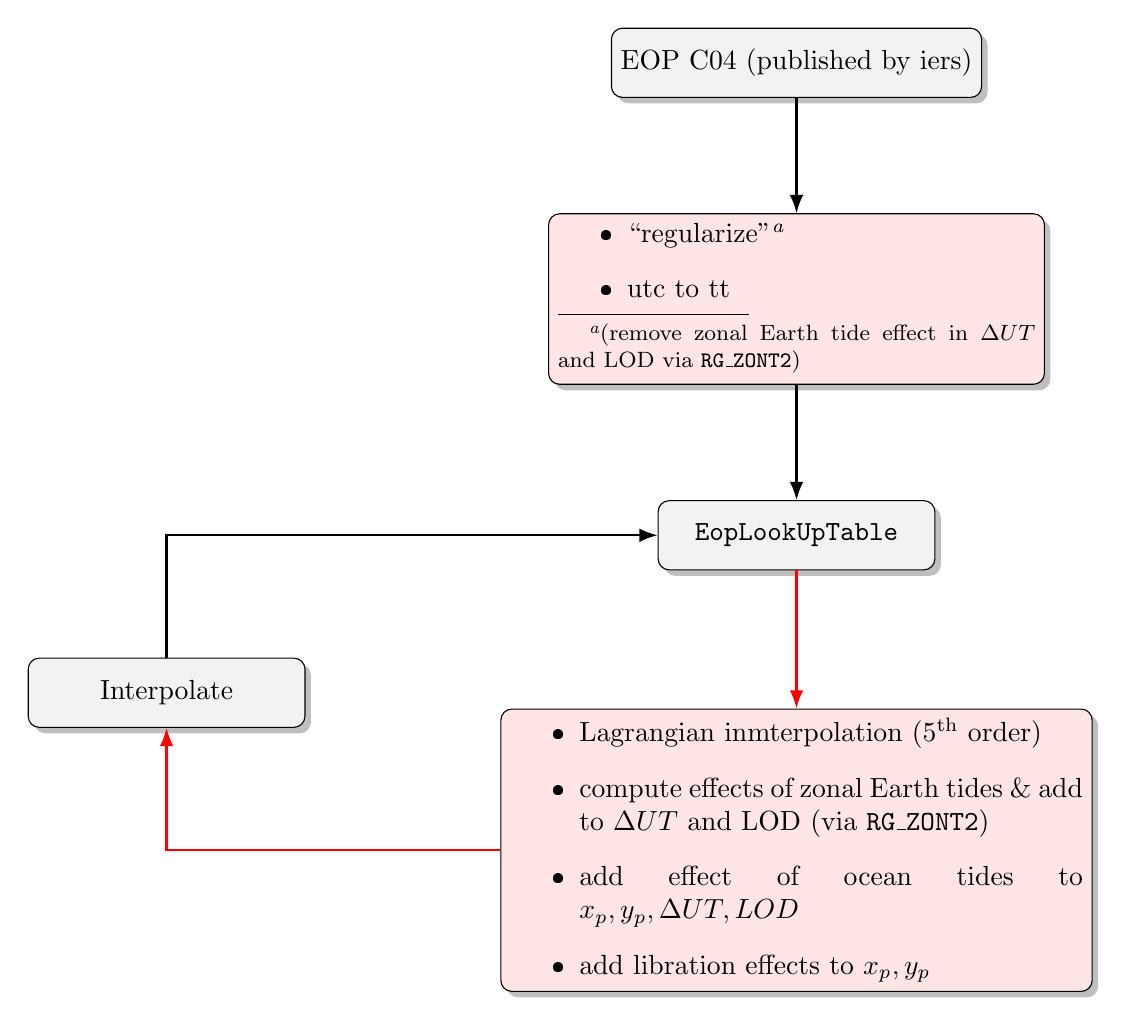
\begin{tikzpicture}
	\node (A) at (0,0) 
		[draw=black, minimum height=2.5em, minimum width=10em, fill=gray!10,rounded corners, drop shadow] 
		{EOP C04 (published by \gls{iers})};
	
	\node (AtB) at (0,-3) 
		[draw=black, minimum height=2.5em, minimum width=10em, fill=red!10,rounded corners, drop shadow]
		{\begin{minipage}{.5\textwidth}\begin{itemize}
		\item ``regularize''\footnote{(remove zonal Earth tide effect in $\Delta UT$ and LOD via \texttt{RG\_ZONT2})}
		\item \gls{utc} to \gls{tt}
		\end{itemize}\end{minipage}};
		
	\node (B) at (0,-6.0) 
		[draw=black, minimum height=2.5em, minimum width=10em, fill=gray!10,rounded corners, drop shadow] 
		{\texttt{EopLookUpTable}};

	\node (BtI) at (0,-10) 
		[draw=black, minimum height=2.5em, minimum width=10em, fill=red!10,rounded corners, drop shadow]
		{\begin{minipage}{.6\textwidth}\begin{itemize}
		\item Lagrangian inmterpolation (5\textsuperscript{th} order)
		\item compute effects of zonal Earth tides \& add to $\Delta UT$ and LOD (via \texttt{RG\_ZONT2})
		\item add effect of ocean tides to $x_p, y_p, \Delta UT, LOD$
		\item add libration effects to $x_p, y_p$
		\end{itemize}\end{minipage}};
	
	\node (I) at (-8,-8)
		[draw=black, minimum height=2.5em, minimum width=10em, fill=gray!10,rounded corners, drop shadow]
		{Interpolate};

	\draw[-Latex,thick] (A.south) -- (AtB.north);
	\draw[-Latex,thick] (AtB.south) -- (B.north);
	\draw[-Latex,thick] (I.north) |- (B.west);
	\draw[-Latex,red,thick] (B.south) -| (BtI.north);
	\draw[-Latex,red,thick] (BtI.west) -| (I.south);
	%\draw[->] (A)--(B) node[midway]{Remove effects of zonal Earth tides on $\Delta$UT and LOD (\texttt{rg\_zont2})}; 
\end{tikzpicture}

  \caption{Extracting and interpolating \gls{eop} information from \gls{iers} 
    \texttt{C04} data files. Red nodes are seamless implicit activities, while 
    green ones are optional, performed on user request.}
  \label{fig:handling-eop}
\end{figure}

Once parsed and stored, one can interpolate \gls{eop} values to any given epoch. 
Interpolation is perfomed using polynomial interpolation, via the \emph{Lagrange} method. 
There are a couple of things going on, to effectively and accuratelly interpolate 
series of \glspl{eop}:
\begin{itemize}
  \item \gls{eop} data should be stored in an \texttt{EopSeries} data structure. 
    Any given instance of this data structure, holds \gls{eop} time series for 
    a given date range.
  \item High frequency effects (i.e. with periods less than one day) have to be 
    taken into consideration when interpolating. These are described in Chapters 
    5.5.1 and 5.5.3 of \cite{iers2010} and \cite{Bradley2016}. These include:
    
    \begin{itemize}
      \item Variations $\Delta _{libration}$, mainly diurnal nutations in 
        polar motion $(x_p, y_p)$, $UT1$ and $LOD$ that originate from the direct 
        effect of the external (mainly luni-solar) torque on the non-axisymmetric 
        part of the Earth. \gls{iers} publishes the 
        \href{https://iers-conventions.obspm.fr/content/chapter5/software/PMSDNUT2.F}{PMSDNUT2} 
        and \href{https://iers-conventions.obspm.fr/content/chapter5/software/UTLIBR.F}{UTLIBR.F} 
        software to model these effects, for polar motion and $UT1$, $LOD$ respectively. 
        %in this library, these computations are performed by the \lstinline{dso::utlod_libration}.

      \item Variations $\Delta _{ocean tides}$ in polar motion $(x_p, y_p)$, $UT1$ and $LOD$; 
        these are tidal variations in Earth orientation, including diurnal and semi-diurnal 
        variations in pole coordinates caused by ocean tides. \gls{iers} publishes the 
        \href{https://iers-conventions.obspm.fr/content/chapter8/software/ORTHO_EOP.F}{ORTHO\_EOP.F} 
        software to model these effects for polar motion.
        %Within this library, the computations are performed by the function \lstinline{dso::xypole_oceantide}.
        
      \item \gls{iers} also publishes the software 
       \href{https://hpiers.obspm.fr/iers/models/interp.f}{interp.f} 
        which is used to interpolate \gls{eop} series. The routine \texttt{pmut1\_oceans} 
        within this software is used to compute the ocean tidal effects while 
        \texttt{pm\_gravi} is used to compute libration effects.

    \end{itemize}

    \item Effects of the tidal deformation (zonal tides) on Earth’s rotation with 
      periods from 5 days to 18.6 years (long-period tides). These affect 
      $\Delta UT1$, $LOD$ and Earth's rotation velocity $\omega$ and are 
      described in Chapter 8.1 of \cite{iers2010}. To model these effects, \gls{iers} 
      publishes the \href{https://iers-conventions.obspm.fr/content/chapter8/software/RG_ZONT2.F}{RG\_ZONT2.F} 
      software.

    \item $\Delta UT1$ has the largest impact on the \gls{itrs}/\gls{gcrs} frame 
      transformation compared to all other \glspl{eop} (\cite{Bradley2016}).  The 
      time difference $\Delta UT1 = UT1-UTC$ contains leap seconds within the data 
      series. This $\pm 1$second jump impacts how the data set should be 
      interpolated and can lead to large errors if done incorrectly (see \autoref{fig:eop-variations}). 
      To overcome this, tabulated $\Delta UT1$ are first transformed to $UT1-TAI$ 
      values via $UT1 - TAI = \Delta UT1 - \Delta AT$, interpolated, and then 
      transformed back to $\Delta UT1$. The procedure is outlined in Section 3.3 of 
      \cite{Bradley2016}.

\end{itemize}

\autoref{lst:eop-interpolation} presents source code to parse, store and 
interpolate \glspl{eop} following the above.

\begin{figure}[h]
  \centering
  %% Creator: Matplotlib, PGF backend
%%
%% To include the figure in your LaTeX document, write
%%   \input{<filename>.pgf}
%%
%% Make sure the required packages are loaded in your preamble
%%   \usepackage{pgf}
%%
%% Also ensure that all the required font packages are loaded; for instance,
%% the lmodern package is sometimes necessary when using math font.
%%   \usepackage{lmodern}
%%
%% Figures using additional raster images can only be included by \input if
%% they are in the same directory as the main LaTeX file. For loading figures
%% from other directories you can use the `import` package
%%   \usepackage{import}
%%
%% and then include the figures with
%%   \import{<path to file>}{<filename>.pgf}
%%
%% Matplotlib used the following preamble
%%   \def\mathdefault#1{#1}
%%   \everymath=\expandafter{\the\everymath\displaystyle}
%%   
%%   \makeatletter\@ifpackageloaded{underscore}{}{\usepackage[strings]{underscore}}\makeatother
%%
\begingroup%
\makeatletter%
\begin{pgfpicture}%
\pgfpathrectangle{\pgfpointorigin}{\pgfqpoint{5.783866in}{3.574626in}}%
\pgfusepath{use as bounding box, clip}%
\begin{pgfscope}%
\pgfsetbuttcap%
\pgfsetmiterjoin%
\definecolor{currentfill}{rgb}{1.000000,1.000000,1.000000}%
\pgfsetfillcolor{currentfill}%
\pgfsetlinewidth{0.000000pt}%
\definecolor{currentstroke}{rgb}{1.000000,1.000000,1.000000}%
\pgfsetstrokecolor{currentstroke}%
\pgfsetdash{}{0pt}%
\pgfpathmoveto{\pgfqpoint{0.000000in}{0.000000in}}%
\pgfpathlineto{\pgfqpoint{5.783866in}{0.000000in}}%
\pgfpathlineto{\pgfqpoint{5.783866in}{3.574626in}}%
\pgfpathlineto{\pgfqpoint{0.000000in}{3.574626in}}%
\pgfpathlineto{\pgfqpoint{0.000000in}{0.000000in}}%
\pgfpathclose%
\pgfusepath{fill}%
\end{pgfscope}%
\begin{pgfscope}%
\pgfsetbuttcap%
\pgfsetmiterjoin%
\definecolor{currentfill}{rgb}{0.933333,0.933333,0.933333}%
\pgfsetfillcolor{currentfill}%
\pgfsetlinewidth{0.000000pt}%
\definecolor{currentstroke}{rgb}{0.000000,0.000000,0.000000}%
\pgfsetstrokecolor{currentstroke}%
\pgfsetstrokeopacity{0.000000}%
\pgfsetdash{}{0pt}%
\pgfpathmoveto{\pgfqpoint{0.524610in}{2.020584in}}%
\pgfpathlineto{\pgfqpoint{2.821393in}{2.020584in}}%
\pgfpathlineto{\pgfqpoint{2.821393in}{3.306385in}}%
\pgfpathlineto{\pgfqpoint{0.524610in}{3.306385in}}%
\pgfpathlineto{\pgfqpoint{0.524610in}{2.020584in}}%
\pgfpathclose%
\pgfusepath{fill}%
\end{pgfscope}%
\begin{pgfscope}%
\pgfpathrectangle{\pgfqpoint{0.524610in}{2.020584in}}{\pgfqpoint{2.296783in}{1.285801in}}%
\pgfusepath{clip}%
\pgfsetbuttcap%
\pgfsetroundjoin%
\pgfsetlinewidth{0.501875pt}%
\definecolor{currentstroke}{rgb}{0.698039,0.698039,0.698039}%
\pgfsetstrokecolor{currentstroke}%
\pgfsetdash{{1.850000pt}{0.800000pt}}{0.000000pt}%
\pgfpathmoveto{\pgfqpoint{0.629009in}{2.020584in}}%
\pgfpathlineto{\pgfqpoint{0.629009in}{3.306385in}}%
\pgfusepath{stroke}%
\end{pgfscope}%
\begin{pgfscope}%
\pgfsetbuttcap%
\pgfsetroundjoin%
\definecolor{currentfill}{rgb}{0.000000,0.000000,0.000000}%
\pgfsetfillcolor{currentfill}%
\pgfsetlinewidth{0.803000pt}%
\definecolor{currentstroke}{rgb}{0.000000,0.000000,0.000000}%
\pgfsetstrokecolor{currentstroke}%
\pgfsetdash{}{0pt}%
\pgfsys@defobject{currentmarker}{\pgfqpoint{0.000000in}{0.000000in}}{\pgfqpoint{0.000000in}{0.048611in}}{%
\pgfpathmoveto{\pgfqpoint{0.000000in}{0.000000in}}%
\pgfpathlineto{\pgfqpoint{0.000000in}{0.048611in}}%
\pgfusepath{stroke,fill}%
}%
\begin{pgfscope}%
\pgfsys@transformshift{0.629009in}{2.020584in}%
\pgfsys@useobject{currentmarker}{}%
\end{pgfscope}%
\end{pgfscope}%
\begin{pgfscope}%
\definecolor{textcolor}{rgb}{0.000000,0.000000,0.000000}%
\pgfsetstrokecolor{textcolor}%
\pgfsetfillcolor{textcolor}%
\pgftext[x=0.629009in,y=1.971973in,,top]{\color{textcolor}{\rmfamily\fontsize{5.000000}{6.000000}\selectfont\catcode`\^=\active\def^{\ifmmode\sp\else\^{}\fi}\catcode`\%=\active\def%{\%}$\mathdefault{56304}$}}%
\end{pgfscope}%
\begin{pgfscope}%
\pgfpathrectangle{\pgfqpoint{0.524610in}{2.020584in}}{\pgfqpoint{2.296783in}{1.285801in}}%
\pgfusepath{clip}%
\pgfsetbuttcap%
\pgfsetroundjoin%
\pgfsetlinewidth{0.501875pt}%
\definecolor{currentstroke}{rgb}{0.698039,0.698039,0.698039}%
\pgfsetstrokecolor{currentstroke}%
\pgfsetdash{{1.850000pt}{0.800000pt}}{0.000000pt}%
\pgfpathmoveto{\pgfqpoint{0.977006in}{2.020584in}}%
\pgfpathlineto{\pgfqpoint{0.977006in}{3.306385in}}%
\pgfusepath{stroke}%
\end{pgfscope}%
\begin{pgfscope}%
\pgfsetbuttcap%
\pgfsetroundjoin%
\definecolor{currentfill}{rgb}{0.000000,0.000000,0.000000}%
\pgfsetfillcolor{currentfill}%
\pgfsetlinewidth{0.803000pt}%
\definecolor{currentstroke}{rgb}{0.000000,0.000000,0.000000}%
\pgfsetstrokecolor{currentstroke}%
\pgfsetdash{}{0pt}%
\pgfsys@defobject{currentmarker}{\pgfqpoint{0.000000in}{0.000000in}}{\pgfqpoint{0.000000in}{0.048611in}}{%
\pgfpathmoveto{\pgfqpoint{0.000000in}{0.000000in}}%
\pgfpathlineto{\pgfqpoint{0.000000in}{0.048611in}}%
\pgfusepath{stroke,fill}%
}%
\begin{pgfscope}%
\pgfsys@transformshift{0.977006in}{2.020584in}%
\pgfsys@useobject{currentmarker}{}%
\end{pgfscope}%
\end{pgfscope}%
\begin{pgfscope}%
\definecolor{textcolor}{rgb}{0.000000,0.000000,0.000000}%
\pgfsetstrokecolor{textcolor}%
\pgfsetfillcolor{textcolor}%
\pgftext[x=0.977006in,y=1.971973in,,top]{\color{textcolor}{\rmfamily\fontsize{5.000000}{6.000000}\selectfont\catcode`\^=\active\def^{\ifmmode\sp\else\^{}\fi}\catcode`\%=\active\def%{\%}$\mathdefault{56305}$}}%
\end{pgfscope}%
\begin{pgfscope}%
\pgfpathrectangle{\pgfqpoint{0.524610in}{2.020584in}}{\pgfqpoint{2.296783in}{1.285801in}}%
\pgfusepath{clip}%
\pgfsetbuttcap%
\pgfsetroundjoin%
\pgfsetlinewidth{0.501875pt}%
\definecolor{currentstroke}{rgb}{0.698039,0.698039,0.698039}%
\pgfsetstrokecolor{currentstroke}%
\pgfsetdash{{1.850000pt}{0.800000pt}}{0.000000pt}%
\pgfpathmoveto{\pgfqpoint{1.325004in}{2.020584in}}%
\pgfpathlineto{\pgfqpoint{1.325004in}{3.306385in}}%
\pgfusepath{stroke}%
\end{pgfscope}%
\begin{pgfscope}%
\pgfsetbuttcap%
\pgfsetroundjoin%
\definecolor{currentfill}{rgb}{0.000000,0.000000,0.000000}%
\pgfsetfillcolor{currentfill}%
\pgfsetlinewidth{0.803000pt}%
\definecolor{currentstroke}{rgb}{0.000000,0.000000,0.000000}%
\pgfsetstrokecolor{currentstroke}%
\pgfsetdash{}{0pt}%
\pgfsys@defobject{currentmarker}{\pgfqpoint{0.000000in}{0.000000in}}{\pgfqpoint{0.000000in}{0.048611in}}{%
\pgfpathmoveto{\pgfqpoint{0.000000in}{0.000000in}}%
\pgfpathlineto{\pgfqpoint{0.000000in}{0.048611in}}%
\pgfusepath{stroke,fill}%
}%
\begin{pgfscope}%
\pgfsys@transformshift{1.325004in}{2.020584in}%
\pgfsys@useobject{currentmarker}{}%
\end{pgfscope}%
\end{pgfscope}%
\begin{pgfscope}%
\definecolor{textcolor}{rgb}{0.000000,0.000000,0.000000}%
\pgfsetstrokecolor{textcolor}%
\pgfsetfillcolor{textcolor}%
\pgftext[x=1.325004in,y=1.971973in,,top]{\color{textcolor}{\rmfamily\fontsize{5.000000}{6.000000}\selectfont\catcode`\^=\active\def^{\ifmmode\sp\else\^{}\fi}\catcode`\%=\active\def%{\%}$\mathdefault{56306}$}}%
\end{pgfscope}%
\begin{pgfscope}%
\pgfpathrectangle{\pgfqpoint{0.524610in}{2.020584in}}{\pgfqpoint{2.296783in}{1.285801in}}%
\pgfusepath{clip}%
\pgfsetbuttcap%
\pgfsetroundjoin%
\pgfsetlinewidth{0.501875pt}%
\definecolor{currentstroke}{rgb}{0.698039,0.698039,0.698039}%
\pgfsetstrokecolor{currentstroke}%
\pgfsetdash{{1.850000pt}{0.800000pt}}{0.000000pt}%
\pgfpathmoveto{\pgfqpoint{1.673001in}{2.020584in}}%
\pgfpathlineto{\pgfqpoint{1.673001in}{3.306385in}}%
\pgfusepath{stroke}%
\end{pgfscope}%
\begin{pgfscope}%
\pgfsetbuttcap%
\pgfsetroundjoin%
\definecolor{currentfill}{rgb}{0.000000,0.000000,0.000000}%
\pgfsetfillcolor{currentfill}%
\pgfsetlinewidth{0.803000pt}%
\definecolor{currentstroke}{rgb}{0.000000,0.000000,0.000000}%
\pgfsetstrokecolor{currentstroke}%
\pgfsetdash{}{0pt}%
\pgfsys@defobject{currentmarker}{\pgfqpoint{0.000000in}{0.000000in}}{\pgfqpoint{0.000000in}{0.048611in}}{%
\pgfpathmoveto{\pgfqpoint{0.000000in}{0.000000in}}%
\pgfpathlineto{\pgfqpoint{0.000000in}{0.048611in}}%
\pgfusepath{stroke,fill}%
}%
\begin{pgfscope}%
\pgfsys@transformshift{1.673001in}{2.020584in}%
\pgfsys@useobject{currentmarker}{}%
\end{pgfscope}%
\end{pgfscope}%
\begin{pgfscope}%
\definecolor{textcolor}{rgb}{0.000000,0.000000,0.000000}%
\pgfsetstrokecolor{textcolor}%
\pgfsetfillcolor{textcolor}%
\pgftext[x=1.673001in,y=1.971973in,,top]{\color{textcolor}{\rmfamily\fontsize{5.000000}{6.000000}\selectfont\catcode`\^=\active\def^{\ifmmode\sp\else\^{}\fi}\catcode`\%=\active\def%{\%}$\mathdefault{56307}$}}%
\end{pgfscope}%
\begin{pgfscope}%
\pgfpathrectangle{\pgfqpoint{0.524610in}{2.020584in}}{\pgfqpoint{2.296783in}{1.285801in}}%
\pgfusepath{clip}%
\pgfsetbuttcap%
\pgfsetroundjoin%
\pgfsetlinewidth{0.501875pt}%
\definecolor{currentstroke}{rgb}{0.698039,0.698039,0.698039}%
\pgfsetstrokecolor{currentstroke}%
\pgfsetdash{{1.850000pt}{0.800000pt}}{0.000000pt}%
\pgfpathmoveto{\pgfqpoint{2.020999in}{2.020584in}}%
\pgfpathlineto{\pgfqpoint{2.020999in}{3.306385in}}%
\pgfusepath{stroke}%
\end{pgfscope}%
\begin{pgfscope}%
\pgfsetbuttcap%
\pgfsetroundjoin%
\definecolor{currentfill}{rgb}{0.000000,0.000000,0.000000}%
\pgfsetfillcolor{currentfill}%
\pgfsetlinewidth{0.803000pt}%
\definecolor{currentstroke}{rgb}{0.000000,0.000000,0.000000}%
\pgfsetstrokecolor{currentstroke}%
\pgfsetdash{}{0pt}%
\pgfsys@defobject{currentmarker}{\pgfqpoint{0.000000in}{0.000000in}}{\pgfqpoint{0.000000in}{0.048611in}}{%
\pgfpathmoveto{\pgfqpoint{0.000000in}{0.000000in}}%
\pgfpathlineto{\pgfqpoint{0.000000in}{0.048611in}}%
\pgfusepath{stroke,fill}%
}%
\begin{pgfscope}%
\pgfsys@transformshift{2.020999in}{2.020584in}%
\pgfsys@useobject{currentmarker}{}%
\end{pgfscope}%
\end{pgfscope}%
\begin{pgfscope}%
\definecolor{textcolor}{rgb}{0.000000,0.000000,0.000000}%
\pgfsetstrokecolor{textcolor}%
\pgfsetfillcolor{textcolor}%
\pgftext[x=2.020999in,y=1.971973in,,top]{\color{textcolor}{\rmfamily\fontsize{5.000000}{6.000000}\selectfont\catcode`\^=\active\def^{\ifmmode\sp\else\^{}\fi}\catcode`\%=\active\def%{\%}$\mathdefault{56308}$}}%
\end{pgfscope}%
\begin{pgfscope}%
\pgfpathrectangle{\pgfqpoint{0.524610in}{2.020584in}}{\pgfqpoint{2.296783in}{1.285801in}}%
\pgfusepath{clip}%
\pgfsetbuttcap%
\pgfsetroundjoin%
\pgfsetlinewidth{0.501875pt}%
\definecolor{currentstroke}{rgb}{0.698039,0.698039,0.698039}%
\pgfsetstrokecolor{currentstroke}%
\pgfsetdash{{1.850000pt}{0.800000pt}}{0.000000pt}%
\pgfpathmoveto{\pgfqpoint{2.368996in}{2.020584in}}%
\pgfpathlineto{\pgfqpoint{2.368996in}{3.306385in}}%
\pgfusepath{stroke}%
\end{pgfscope}%
\begin{pgfscope}%
\pgfsetbuttcap%
\pgfsetroundjoin%
\definecolor{currentfill}{rgb}{0.000000,0.000000,0.000000}%
\pgfsetfillcolor{currentfill}%
\pgfsetlinewidth{0.803000pt}%
\definecolor{currentstroke}{rgb}{0.000000,0.000000,0.000000}%
\pgfsetstrokecolor{currentstroke}%
\pgfsetdash{}{0pt}%
\pgfsys@defobject{currentmarker}{\pgfqpoint{0.000000in}{0.000000in}}{\pgfqpoint{0.000000in}{0.048611in}}{%
\pgfpathmoveto{\pgfqpoint{0.000000in}{0.000000in}}%
\pgfpathlineto{\pgfqpoint{0.000000in}{0.048611in}}%
\pgfusepath{stroke,fill}%
}%
\begin{pgfscope}%
\pgfsys@transformshift{2.368996in}{2.020584in}%
\pgfsys@useobject{currentmarker}{}%
\end{pgfscope}%
\end{pgfscope}%
\begin{pgfscope}%
\definecolor{textcolor}{rgb}{0.000000,0.000000,0.000000}%
\pgfsetstrokecolor{textcolor}%
\pgfsetfillcolor{textcolor}%
\pgftext[x=2.368996in,y=1.971973in,,top]{\color{textcolor}{\rmfamily\fontsize{5.000000}{6.000000}\selectfont\catcode`\^=\active\def^{\ifmmode\sp\else\^{}\fi}\catcode`\%=\active\def%{\%}$\mathdefault{56309}$}}%
\end{pgfscope}%
\begin{pgfscope}%
\pgfpathrectangle{\pgfqpoint{0.524610in}{2.020584in}}{\pgfqpoint{2.296783in}{1.285801in}}%
\pgfusepath{clip}%
\pgfsetbuttcap%
\pgfsetroundjoin%
\pgfsetlinewidth{0.501875pt}%
\definecolor{currentstroke}{rgb}{0.698039,0.698039,0.698039}%
\pgfsetstrokecolor{currentstroke}%
\pgfsetdash{{1.850000pt}{0.800000pt}}{0.000000pt}%
\pgfpathmoveto{\pgfqpoint{2.716993in}{2.020584in}}%
\pgfpathlineto{\pgfqpoint{2.716993in}{3.306385in}}%
\pgfusepath{stroke}%
\end{pgfscope}%
\begin{pgfscope}%
\pgfsetbuttcap%
\pgfsetroundjoin%
\definecolor{currentfill}{rgb}{0.000000,0.000000,0.000000}%
\pgfsetfillcolor{currentfill}%
\pgfsetlinewidth{0.803000pt}%
\definecolor{currentstroke}{rgb}{0.000000,0.000000,0.000000}%
\pgfsetstrokecolor{currentstroke}%
\pgfsetdash{}{0pt}%
\pgfsys@defobject{currentmarker}{\pgfqpoint{0.000000in}{0.000000in}}{\pgfqpoint{0.000000in}{0.048611in}}{%
\pgfpathmoveto{\pgfqpoint{0.000000in}{0.000000in}}%
\pgfpathlineto{\pgfqpoint{0.000000in}{0.048611in}}%
\pgfusepath{stroke,fill}%
}%
\begin{pgfscope}%
\pgfsys@transformshift{2.716993in}{2.020584in}%
\pgfsys@useobject{currentmarker}{}%
\end{pgfscope}%
\end{pgfscope}%
\begin{pgfscope}%
\definecolor{textcolor}{rgb}{0.000000,0.000000,0.000000}%
\pgfsetstrokecolor{textcolor}%
\pgfsetfillcolor{textcolor}%
\pgftext[x=2.716993in,y=1.971973in,,top]{\color{textcolor}{\rmfamily\fontsize{5.000000}{6.000000}\selectfont\catcode`\^=\active\def^{\ifmmode\sp\else\^{}\fi}\catcode`\%=\active\def%{\%}$\mathdefault{56310}$}}%
\end{pgfscope}%
\begin{pgfscope}%
\pgfpathrectangle{\pgfqpoint{0.524610in}{2.020584in}}{\pgfqpoint{2.296783in}{1.285801in}}%
\pgfusepath{clip}%
\pgfsetbuttcap%
\pgfsetroundjoin%
\pgfsetlinewidth{0.501875pt}%
\definecolor{currentstroke}{rgb}{0.698039,0.698039,0.698039}%
\pgfsetstrokecolor{currentstroke}%
\pgfsetdash{{1.850000pt}{0.800000pt}}{0.000000pt}%
\pgfpathmoveto{\pgfqpoint{0.524610in}{2.130196in}}%
\pgfpathlineto{\pgfqpoint{2.821393in}{2.130196in}}%
\pgfusepath{stroke}%
\end{pgfscope}%
\begin{pgfscope}%
\pgfsetbuttcap%
\pgfsetroundjoin%
\definecolor{currentfill}{rgb}{0.000000,0.000000,0.000000}%
\pgfsetfillcolor{currentfill}%
\pgfsetlinewidth{0.803000pt}%
\definecolor{currentstroke}{rgb}{0.000000,0.000000,0.000000}%
\pgfsetstrokecolor{currentstroke}%
\pgfsetdash{}{0pt}%
\pgfsys@defobject{currentmarker}{\pgfqpoint{0.000000in}{0.000000in}}{\pgfqpoint{0.048611in}{0.000000in}}{%
\pgfpathmoveto{\pgfqpoint{0.000000in}{0.000000in}}%
\pgfpathlineto{\pgfqpoint{0.048611in}{0.000000in}}%
\pgfusepath{stroke,fill}%
}%
\begin{pgfscope}%
\pgfsys@transformshift{0.524610in}{2.130196in}%
\pgfsys@useobject{currentmarker}{}%
\end{pgfscope}%
\end{pgfscope}%
\begin{pgfscope}%
\definecolor{textcolor}{rgb}{0.000000,0.000000,0.000000}%
\pgfsetstrokecolor{textcolor}%
\pgfsetfillcolor{textcolor}%
\pgftext[x=0.258982in, y=2.106084in, left, base]{\color{textcolor}{\rmfamily\fontsize{5.000000}{6.000000}\selectfont\catcode`\^=\active\def^{\ifmmode\sp\else\^{}\fi}\catcode`\%=\active\def%{\%}$\mathdefault{\ensuremath{-}600}$}}%
\end{pgfscope}%
\begin{pgfscope}%
\pgfpathrectangle{\pgfqpoint{0.524610in}{2.020584in}}{\pgfqpoint{2.296783in}{1.285801in}}%
\pgfusepath{clip}%
\pgfsetbuttcap%
\pgfsetroundjoin%
\pgfsetlinewidth{0.501875pt}%
\definecolor{currentstroke}{rgb}{0.698039,0.698039,0.698039}%
\pgfsetstrokecolor{currentstroke}%
\pgfsetdash{{1.850000pt}{0.800000pt}}{0.000000pt}%
\pgfpathmoveto{\pgfqpoint{0.524610in}{2.286437in}}%
\pgfpathlineto{\pgfqpoint{2.821393in}{2.286437in}}%
\pgfusepath{stroke}%
\end{pgfscope}%
\begin{pgfscope}%
\pgfsetbuttcap%
\pgfsetroundjoin%
\definecolor{currentfill}{rgb}{0.000000,0.000000,0.000000}%
\pgfsetfillcolor{currentfill}%
\pgfsetlinewidth{0.803000pt}%
\definecolor{currentstroke}{rgb}{0.000000,0.000000,0.000000}%
\pgfsetstrokecolor{currentstroke}%
\pgfsetdash{}{0pt}%
\pgfsys@defobject{currentmarker}{\pgfqpoint{0.000000in}{0.000000in}}{\pgfqpoint{0.048611in}{0.000000in}}{%
\pgfpathmoveto{\pgfqpoint{0.000000in}{0.000000in}}%
\pgfpathlineto{\pgfqpoint{0.048611in}{0.000000in}}%
\pgfusepath{stroke,fill}%
}%
\begin{pgfscope}%
\pgfsys@transformshift{0.524610in}{2.286437in}%
\pgfsys@useobject{currentmarker}{}%
\end{pgfscope}%
\end{pgfscope}%
\begin{pgfscope}%
\definecolor{textcolor}{rgb}{0.000000,0.000000,0.000000}%
\pgfsetstrokecolor{textcolor}%
\pgfsetfillcolor{textcolor}%
\pgftext[x=0.258982in, y=2.262325in, left, base]{\color{textcolor}{\rmfamily\fontsize{5.000000}{6.000000}\selectfont\catcode`\^=\active\def^{\ifmmode\sp\else\^{}\fi}\catcode`\%=\active\def%{\%}$\mathdefault{\ensuremath{-}400}$}}%
\end{pgfscope}%
\begin{pgfscope}%
\pgfpathrectangle{\pgfqpoint{0.524610in}{2.020584in}}{\pgfqpoint{2.296783in}{1.285801in}}%
\pgfusepath{clip}%
\pgfsetbuttcap%
\pgfsetroundjoin%
\pgfsetlinewidth{0.501875pt}%
\definecolor{currentstroke}{rgb}{0.698039,0.698039,0.698039}%
\pgfsetstrokecolor{currentstroke}%
\pgfsetdash{{1.850000pt}{0.800000pt}}{0.000000pt}%
\pgfpathmoveto{\pgfqpoint{0.524610in}{2.442678in}}%
\pgfpathlineto{\pgfqpoint{2.821393in}{2.442678in}}%
\pgfusepath{stroke}%
\end{pgfscope}%
\begin{pgfscope}%
\pgfsetbuttcap%
\pgfsetroundjoin%
\definecolor{currentfill}{rgb}{0.000000,0.000000,0.000000}%
\pgfsetfillcolor{currentfill}%
\pgfsetlinewidth{0.803000pt}%
\definecolor{currentstroke}{rgb}{0.000000,0.000000,0.000000}%
\pgfsetstrokecolor{currentstroke}%
\pgfsetdash{}{0pt}%
\pgfsys@defobject{currentmarker}{\pgfqpoint{0.000000in}{0.000000in}}{\pgfqpoint{0.048611in}{0.000000in}}{%
\pgfpathmoveto{\pgfqpoint{0.000000in}{0.000000in}}%
\pgfpathlineto{\pgfqpoint{0.048611in}{0.000000in}}%
\pgfusepath{stroke,fill}%
}%
\begin{pgfscope}%
\pgfsys@transformshift{0.524610in}{2.442678in}%
\pgfsys@useobject{currentmarker}{}%
\end{pgfscope}%
\end{pgfscope}%
\begin{pgfscope}%
\definecolor{textcolor}{rgb}{0.000000,0.000000,0.000000}%
\pgfsetstrokecolor{textcolor}%
\pgfsetfillcolor{textcolor}%
\pgftext[x=0.258982in, y=2.418566in, left, base]{\color{textcolor}{\rmfamily\fontsize{5.000000}{6.000000}\selectfont\catcode`\^=\active\def^{\ifmmode\sp\else\^{}\fi}\catcode`\%=\active\def%{\%}$\mathdefault{\ensuremath{-}200}$}}%
\end{pgfscope}%
\begin{pgfscope}%
\pgfpathrectangle{\pgfqpoint{0.524610in}{2.020584in}}{\pgfqpoint{2.296783in}{1.285801in}}%
\pgfusepath{clip}%
\pgfsetbuttcap%
\pgfsetroundjoin%
\pgfsetlinewidth{0.501875pt}%
\definecolor{currentstroke}{rgb}{0.698039,0.698039,0.698039}%
\pgfsetstrokecolor{currentstroke}%
\pgfsetdash{{1.850000pt}{0.800000pt}}{0.000000pt}%
\pgfpathmoveto{\pgfqpoint{0.524610in}{2.598919in}}%
\pgfpathlineto{\pgfqpoint{2.821393in}{2.598919in}}%
\pgfusepath{stroke}%
\end{pgfscope}%
\begin{pgfscope}%
\pgfsetbuttcap%
\pgfsetroundjoin%
\definecolor{currentfill}{rgb}{0.000000,0.000000,0.000000}%
\pgfsetfillcolor{currentfill}%
\pgfsetlinewidth{0.803000pt}%
\definecolor{currentstroke}{rgb}{0.000000,0.000000,0.000000}%
\pgfsetstrokecolor{currentstroke}%
\pgfsetdash{}{0pt}%
\pgfsys@defobject{currentmarker}{\pgfqpoint{0.000000in}{0.000000in}}{\pgfqpoint{0.048611in}{0.000000in}}{%
\pgfpathmoveto{\pgfqpoint{0.000000in}{0.000000in}}%
\pgfpathlineto{\pgfqpoint{0.048611in}{0.000000in}}%
\pgfusepath{stroke,fill}%
}%
\begin{pgfscope}%
\pgfsys@transformshift{0.524610in}{2.598919in}%
\pgfsys@useobject{currentmarker}{}%
\end{pgfscope}%
\end{pgfscope}%
\begin{pgfscope}%
\definecolor{textcolor}{rgb}{0.000000,0.000000,0.000000}%
\pgfsetstrokecolor{textcolor}%
\pgfsetfillcolor{textcolor}%
\pgftext[x=0.428737in, y=2.574807in, left, base]{\color{textcolor}{\rmfamily\fontsize{5.000000}{6.000000}\selectfont\catcode`\^=\active\def^{\ifmmode\sp\else\^{}\fi}\catcode`\%=\active\def%{\%}$\mathdefault{0}$}}%
\end{pgfscope}%
\begin{pgfscope}%
\pgfpathrectangle{\pgfqpoint{0.524610in}{2.020584in}}{\pgfqpoint{2.296783in}{1.285801in}}%
\pgfusepath{clip}%
\pgfsetbuttcap%
\pgfsetroundjoin%
\pgfsetlinewidth{0.501875pt}%
\definecolor{currentstroke}{rgb}{0.698039,0.698039,0.698039}%
\pgfsetstrokecolor{currentstroke}%
\pgfsetdash{{1.850000pt}{0.800000pt}}{0.000000pt}%
\pgfpathmoveto{\pgfqpoint{0.524610in}{2.755160in}}%
\pgfpathlineto{\pgfqpoint{2.821393in}{2.755160in}}%
\pgfusepath{stroke}%
\end{pgfscope}%
\begin{pgfscope}%
\pgfsetbuttcap%
\pgfsetroundjoin%
\definecolor{currentfill}{rgb}{0.000000,0.000000,0.000000}%
\pgfsetfillcolor{currentfill}%
\pgfsetlinewidth{0.803000pt}%
\definecolor{currentstroke}{rgb}{0.000000,0.000000,0.000000}%
\pgfsetstrokecolor{currentstroke}%
\pgfsetdash{}{0pt}%
\pgfsys@defobject{currentmarker}{\pgfqpoint{0.000000in}{0.000000in}}{\pgfqpoint{0.048611in}{0.000000in}}{%
\pgfpathmoveto{\pgfqpoint{0.000000in}{0.000000in}}%
\pgfpathlineto{\pgfqpoint{0.048611in}{0.000000in}}%
\pgfusepath{stroke,fill}%
}%
\begin{pgfscope}%
\pgfsys@transformshift{0.524610in}{2.755160in}%
\pgfsys@useobject{currentmarker}{}%
\end{pgfscope}%
\end{pgfscope}%
\begin{pgfscope}%
\definecolor{textcolor}{rgb}{0.000000,0.000000,0.000000}%
\pgfsetstrokecolor{textcolor}%
\pgfsetfillcolor{textcolor}%
\pgftext[x=0.334214in, y=2.731048in, left, base]{\color{textcolor}{\rmfamily\fontsize{5.000000}{6.000000}\selectfont\catcode`\^=\active\def^{\ifmmode\sp\else\^{}\fi}\catcode`\%=\active\def%{\%}$\mathdefault{200}$}}%
\end{pgfscope}%
\begin{pgfscope}%
\pgfpathrectangle{\pgfqpoint{0.524610in}{2.020584in}}{\pgfqpoint{2.296783in}{1.285801in}}%
\pgfusepath{clip}%
\pgfsetbuttcap%
\pgfsetroundjoin%
\pgfsetlinewidth{0.501875pt}%
\definecolor{currentstroke}{rgb}{0.698039,0.698039,0.698039}%
\pgfsetstrokecolor{currentstroke}%
\pgfsetdash{{1.850000pt}{0.800000pt}}{0.000000pt}%
\pgfpathmoveto{\pgfqpoint{0.524610in}{2.911401in}}%
\pgfpathlineto{\pgfqpoint{2.821393in}{2.911401in}}%
\pgfusepath{stroke}%
\end{pgfscope}%
\begin{pgfscope}%
\pgfsetbuttcap%
\pgfsetroundjoin%
\definecolor{currentfill}{rgb}{0.000000,0.000000,0.000000}%
\pgfsetfillcolor{currentfill}%
\pgfsetlinewidth{0.803000pt}%
\definecolor{currentstroke}{rgb}{0.000000,0.000000,0.000000}%
\pgfsetstrokecolor{currentstroke}%
\pgfsetdash{}{0pt}%
\pgfsys@defobject{currentmarker}{\pgfqpoint{0.000000in}{0.000000in}}{\pgfqpoint{0.048611in}{0.000000in}}{%
\pgfpathmoveto{\pgfqpoint{0.000000in}{0.000000in}}%
\pgfpathlineto{\pgfqpoint{0.048611in}{0.000000in}}%
\pgfusepath{stroke,fill}%
}%
\begin{pgfscope}%
\pgfsys@transformshift{0.524610in}{2.911401in}%
\pgfsys@useobject{currentmarker}{}%
\end{pgfscope}%
\end{pgfscope}%
\begin{pgfscope}%
\definecolor{textcolor}{rgb}{0.000000,0.000000,0.000000}%
\pgfsetstrokecolor{textcolor}%
\pgfsetfillcolor{textcolor}%
\pgftext[x=0.334214in, y=2.887289in, left, base]{\color{textcolor}{\rmfamily\fontsize{5.000000}{6.000000}\selectfont\catcode`\^=\active\def^{\ifmmode\sp\else\^{}\fi}\catcode`\%=\active\def%{\%}$\mathdefault{400}$}}%
\end{pgfscope}%
\begin{pgfscope}%
\pgfpathrectangle{\pgfqpoint{0.524610in}{2.020584in}}{\pgfqpoint{2.296783in}{1.285801in}}%
\pgfusepath{clip}%
\pgfsetbuttcap%
\pgfsetroundjoin%
\pgfsetlinewidth{0.501875pt}%
\definecolor{currentstroke}{rgb}{0.698039,0.698039,0.698039}%
\pgfsetstrokecolor{currentstroke}%
\pgfsetdash{{1.850000pt}{0.800000pt}}{0.000000pt}%
\pgfpathmoveto{\pgfqpoint{0.524610in}{3.067642in}}%
\pgfpathlineto{\pgfqpoint{2.821393in}{3.067642in}}%
\pgfusepath{stroke}%
\end{pgfscope}%
\begin{pgfscope}%
\pgfsetbuttcap%
\pgfsetroundjoin%
\definecolor{currentfill}{rgb}{0.000000,0.000000,0.000000}%
\pgfsetfillcolor{currentfill}%
\pgfsetlinewidth{0.803000pt}%
\definecolor{currentstroke}{rgb}{0.000000,0.000000,0.000000}%
\pgfsetstrokecolor{currentstroke}%
\pgfsetdash{}{0pt}%
\pgfsys@defobject{currentmarker}{\pgfqpoint{0.000000in}{0.000000in}}{\pgfqpoint{0.048611in}{0.000000in}}{%
\pgfpathmoveto{\pgfqpoint{0.000000in}{0.000000in}}%
\pgfpathlineto{\pgfqpoint{0.048611in}{0.000000in}}%
\pgfusepath{stroke,fill}%
}%
\begin{pgfscope}%
\pgfsys@transformshift{0.524610in}{3.067642in}%
\pgfsys@useobject{currentmarker}{}%
\end{pgfscope}%
\end{pgfscope}%
\begin{pgfscope}%
\definecolor{textcolor}{rgb}{0.000000,0.000000,0.000000}%
\pgfsetstrokecolor{textcolor}%
\pgfsetfillcolor{textcolor}%
\pgftext[x=0.334214in, y=3.043530in, left, base]{\color{textcolor}{\rmfamily\fontsize{5.000000}{6.000000}\selectfont\catcode`\^=\active\def^{\ifmmode\sp\else\^{}\fi}\catcode`\%=\active\def%{\%}$\mathdefault{600}$}}%
\end{pgfscope}%
\begin{pgfscope}%
\pgfpathrectangle{\pgfqpoint{0.524610in}{2.020584in}}{\pgfqpoint{2.296783in}{1.285801in}}%
\pgfusepath{clip}%
\pgfsetbuttcap%
\pgfsetroundjoin%
\pgfsetlinewidth{0.501875pt}%
\definecolor{currentstroke}{rgb}{0.698039,0.698039,0.698039}%
\pgfsetstrokecolor{currentstroke}%
\pgfsetdash{{1.850000pt}{0.800000pt}}{0.000000pt}%
\pgfpathmoveto{\pgfqpoint{0.524610in}{3.223883in}}%
\pgfpathlineto{\pgfqpoint{2.821393in}{3.223883in}}%
\pgfusepath{stroke}%
\end{pgfscope}%
\begin{pgfscope}%
\pgfsetbuttcap%
\pgfsetroundjoin%
\definecolor{currentfill}{rgb}{0.000000,0.000000,0.000000}%
\pgfsetfillcolor{currentfill}%
\pgfsetlinewidth{0.803000pt}%
\definecolor{currentstroke}{rgb}{0.000000,0.000000,0.000000}%
\pgfsetstrokecolor{currentstroke}%
\pgfsetdash{}{0pt}%
\pgfsys@defobject{currentmarker}{\pgfqpoint{0.000000in}{0.000000in}}{\pgfqpoint{0.048611in}{0.000000in}}{%
\pgfpathmoveto{\pgfqpoint{0.000000in}{0.000000in}}%
\pgfpathlineto{\pgfqpoint{0.048611in}{0.000000in}}%
\pgfusepath{stroke,fill}%
}%
\begin{pgfscope}%
\pgfsys@transformshift{0.524610in}{3.223883in}%
\pgfsys@useobject{currentmarker}{}%
\end{pgfscope}%
\end{pgfscope}%
\begin{pgfscope}%
\definecolor{textcolor}{rgb}{0.000000,0.000000,0.000000}%
\pgfsetstrokecolor{textcolor}%
\pgfsetfillcolor{textcolor}%
\pgftext[x=0.334214in, y=3.199771in, left, base]{\color{textcolor}{\rmfamily\fontsize{5.000000}{6.000000}\selectfont\catcode`\^=\active\def^{\ifmmode\sp\else\^{}\fi}\catcode`\%=\active\def%{\%}$\mathdefault{800}$}}%
\end{pgfscope}%
\begin{pgfscope}%
\definecolor{textcolor}{rgb}{0.000000,0.000000,0.000000}%
\pgfsetstrokecolor{textcolor}%
\pgfsetfillcolor{textcolor}%
\pgftext[x=0.203426in,y=2.663485in,,bottom,rotate=90.000000]{\color{textcolor}{\rmfamily\fontsize{8.000000}{9.600000}\selectfont\catcode`\^=\active\def^{\ifmmode\sp\else\^{}\fi}\catcode`\%=\active\def%{\%}$\Delta x_p$ in $[\mu arcsec]$}}%
\end{pgfscope}%
\begin{pgfscope}%
\pgfpathrectangle{\pgfqpoint{0.524610in}{2.020584in}}{\pgfqpoint{2.296783in}{1.285801in}}%
\pgfusepath{clip}%
\pgfsetrectcap%
\pgfsetroundjoin%
\pgfsetlinewidth{1.003750pt}%
\definecolor{currentstroke}{rgb}{0.203922,0.541176,0.741176}%
\pgfsetstrokecolor{currentstroke}%
\pgfsetdash{}{0pt}%
\pgfpathmoveto{\pgfqpoint{0.629009in}{2.786416in}}%
\pgfpathlineto{\pgfqpoint{0.653369in}{2.350444in}}%
\pgfpathlineto{\pgfqpoint{0.663809in}{2.208149in}}%
\pgfpathlineto{\pgfqpoint{0.670769in}{2.140032in}}%
\pgfpathlineto{\pgfqpoint{0.677729in}{2.096583in}}%
\pgfpathlineto{\pgfqpoint{0.681209in}{2.084551in}}%
\pgfpathlineto{\pgfqpoint{0.684689in}{2.079030in}}%
\pgfpathlineto{\pgfqpoint{0.688169in}{2.079943in}}%
\pgfpathlineto{\pgfqpoint{0.691648in}{2.087123in}}%
\pgfpathlineto{\pgfqpoint{0.695128in}{2.100312in}}%
\pgfpathlineto{\pgfqpoint{0.702088in}{2.143284in}}%
\pgfpathlineto{\pgfqpoint{0.709048in}{2.205247in}}%
\pgfpathlineto{\pgfqpoint{0.719488in}{2.323485in}}%
\pgfpathlineto{\pgfqpoint{0.743848in}{2.619877in}}%
\pgfpathlineto{\pgfqpoint{0.750808in}{2.685212in}}%
\pgfpathlineto{\pgfqpoint{0.757768in}{2.733812in}}%
\pgfpathlineto{\pgfqpoint{0.764728in}{2.762926in}}%
\pgfpathlineto{\pgfqpoint{0.768208in}{2.769676in}}%
\pgfpathlineto{\pgfqpoint{0.771688in}{2.771129in}}%
\pgfpathlineto{\pgfqpoint{0.775168in}{2.767326in}}%
\pgfpathlineto{\pgfqpoint{0.778648in}{2.758400in}}%
\pgfpathlineto{\pgfqpoint{0.782128in}{2.744565in}}%
\pgfpathlineto{\pgfqpoint{0.789088in}{2.703445in}}%
\pgfpathlineto{\pgfqpoint{0.796048in}{2.647254in}}%
\pgfpathlineto{\pgfqpoint{0.809968in}{2.507678in}}%
\pgfpathlineto{\pgfqpoint{0.823887in}{2.367493in}}%
\pgfpathlineto{\pgfqpoint{0.830847in}{2.310881in}}%
\pgfpathlineto{\pgfqpoint{0.837807in}{2.269777in}}%
\pgfpathlineto{\pgfqpoint{0.841287in}{2.256284in}}%
\pgfpathlineto{\pgfqpoint{0.844767in}{2.248022in}}%
\pgfpathlineto{\pgfqpoint{0.848247in}{2.245290in}}%
\pgfpathlineto{\pgfqpoint{0.851727in}{2.248300in}}%
\pgfpathlineto{\pgfqpoint{0.855207in}{2.257180in}}%
\pgfpathlineto{\pgfqpoint{0.858687in}{2.271963in}}%
\pgfpathlineto{\pgfqpoint{0.865647in}{2.318924in}}%
\pgfpathlineto{\pgfqpoint{0.872607in}{2.387645in}}%
\pgfpathlineto{\pgfqpoint{0.883047in}{2.524799in}}%
\pgfpathlineto{\pgfqpoint{0.900447in}{2.804821in}}%
\pgfpathlineto{\pgfqpoint{0.914367in}{3.022231in}}%
\pgfpathlineto{\pgfqpoint{0.924807in}{3.149839in}}%
\pgfpathlineto{\pgfqpoint{0.931767in}{3.208468in}}%
\pgfpathlineto{\pgfqpoint{0.935247in}{3.228407in}}%
\pgfpathlineto{\pgfqpoint{0.938727in}{3.241641in}}%
\pgfpathlineto{\pgfqpoint{0.942207in}{3.247940in}}%
\pgfpathlineto{\pgfqpoint{0.945687in}{3.247169in}}%
\pgfpathlineto{\pgfqpoint{0.949167in}{3.239287in}}%
\pgfpathlineto{\pgfqpoint{0.952647in}{3.224353in}}%
\pgfpathlineto{\pgfqpoint{0.959606in}{3.174034in}}%
\pgfpathlineto{\pgfqpoint{0.966566in}{3.098548in}}%
\pgfpathlineto{\pgfqpoint{0.977006in}{2.946565in}}%
\pgfpathlineto{\pgfqpoint{0.990926in}{2.699408in}}%
\pgfpathlineto{\pgfqpoint{1.008326in}{2.389368in}}%
\pgfpathlineto{\pgfqpoint{1.018766in}{2.239693in}}%
\pgfpathlineto{\pgfqpoint{1.025726in}{2.165504in}}%
\pgfpathlineto{\pgfqpoint{1.032686in}{2.115678in}}%
\pgfpathlineto{\pgfqpoint{1.036166in}{2.100508in}}%
\pgfpathlineto{\pgfqpoint{1.039646in}{2.091971in}}%
\pgfpathlineto{\pgfqpoint{1.043126in}{2.090048in}}%
\pgfpathlineto{\pgfqpoint{1.046606in}{2.094630in}}%
\pgfpathlineto{\pgfqpoint{1.050086in}{2.105512in}}%
\pgfpathlineto{\pgfqpoint{1.053566in}{2.122402in}}%
\pgfpathlineto{\pgfqpoint{1.060526in}{2.172615in}}%
\pgfpathlineto{\pgfqpoint{1.067486in}{2.241364in}}%
\pgfpathlineto{\pgfqpoint{1.077926in}{2.368316in}}%
\pgfpathlineto{\pgfqpoint{1.102285in}{2.674687in}}%
\pgfpathlineto{\pgfqpoint{1.109245in}{2.739771in}}%
\pgfpathlineto{\pgfqpoint{1.116205in}{2.786776in}}%
\pgfpathlineto{\pgfqpoint{1.119685in}{2.802624in}}%
\pgfpathlineto{\pgfqpoint{1.123165in}{2.813072in}}%
\pgfpathlineto{\pgfqpoint{1.126645in}{2.818006in}}%
\pgfpathlineto{\pgfqpoint{1.130125in}{2.817406in}}%
\pgfpathlineto{\pgfqpoint{1.133605in}{2.811341in}}%
\pgfpathlineto{\pgfqpoint{1.137085in}{2.799970in}}%
\pgfpathlineto{\pgfqpoint{1.144045in}{2.762378in}}%
\pgfpathlineto{\pgfqpoint{1.151005in}{2.707564in}}%
\pgfpathlineto{\pgfqpoint{1.161445in}{2.602186in}}%
\pgfpathlineto{\pgfqpoint{1.185805in}{2.341264in}}%
\pgfpathlineto{\pgfqpoint{1.192765in}{2.287651in}}%
\pgfpathlineto{\pgfqpoint{1.199725in}{2.252033in}}%
\pgfpathlineto{\pgfqpoint{1.203205in}{2.242025in}}%
\pgfpathlineto{\pgfqpoint{1.206685in}{2.237626in}}%
\pgfpathlineto{\pgfqpoint{1.210165in}{2.239036in}}%
\pgfpathlineto{\pgfqpoint{1.213645in}{2.246363in}}%
\pgfpathlineto{\pgfqpoint{1.217125in}{2.259627in}}%
\pgfpathlineto{\pgfqpoint{1.224085in}{2.303583in}}%
\pgfpathlineto{\pgfqpoint{1.231044in}{2.369232in}}%
\pgfpathlineto{\pgfqpoint{1.241484in}{2.501415in}}%
\pgfpathlineto{\pgfqpoint{1.258884in}{2.771693in}}%
\pgfpathlineto{\pgfqpoint{1.272804in}{2.980234in}}%
\pgfpathlineto{\pgfqpoint{1.283244in}{3.101224in}}%
\pgfpathlineto{\pgfqpoint{1.290204in}{3.155839in}}%
\pgfpathlineto{\pgfqpoint{1.293684in}{3.173981in}}%
\pgfpathlineto{\pgfqpoint{1.297164in}{3.185601in}}%
\pgfpathlineto{\pgfqpoint{1.300644in}{3.190500in}}%
\pgfpathlineto{\pgfqpoint{1.304124in}{3.188574in}}%
\pgfpathlineto{\pgfqpoint{1.307604in}{3.179813in}}%
\pgfpathlineto{\pgfqpoint{1.311084in}{3.164303in}}%
\pgfpathlineto{\pgfqpoint{1.318044in}{3.113840in}}%
\pgfpathlineto{\pgfqpoint{1.325004in}{3.039692in}}%
\pgfpathlineto{\pgfqpoint{1.335444in}{2.892716in}}%
\pgfpathlineto{\pgfqpoint{1.352844in}{2.597214in}}%
\pgfpathlineto{\pgfqpoint{1.366763in}{2.370582in}}%
\pgfpathlineto{\pgfqpoint{1.377203in}{2.236938in}}%
\pgfpathlineto{\pgfqpoint{1.384163in}{2.173675in}}%
\pgfpathlineto{\pgfqpoint{1.391123in}{2.134513in}}%
\pgfpathlineto{\pgfqpoint{1.394603in}{2.124457in}}%
\pgfpathlineto{\pgfqpoint{1.398083in}{2.120826in}}%
\pgfpathlineto{\pgfqpoint{1.401563in}{2.123561in}}%
\pgfpathlineto{\pgfqpoint{1.405043in}{2.132511in}}%
\pgfpathlineto{\pgfqpoint{1.408523in}{2.147437in}}%
\pgfpathlineto{\pgfqpoint{1.415483in}{2.193839in}}%
\pgfpathlineto{\pgfqpoint{1.422443in}{2.259258in}}%
\pgfpathlineto{\pgfqpoint{1.432883in}{2.382874in}}%
\pgfpathlineto{\pgfqpoint{1.457243in}{2.692773in}}%
\pgfpathlineto{\pgfqpoint{1.464203in}{2.761915in}}%
\pgfpathlineto{\pgfqpoint{1.471163in}{2.814055in}}%
\pgfpathlineto{\pgfqpoint{1.478123in}{2.846257in}}%
\pgfpathlineto{\pgfqpoint{1.481603in}{2.854317in}}%
\pgfpathlineto{\pgfqpoint{1.485083in}{2.856887in}}%
\pgfpathlineto{\pgfqpoint{1.488563in}{2.853981in}}%
\pgfpathlineto{\pgfqpoint{1.492043in}{2.845701in}}%
\pgfpathlineto{\pgfqpoint{1.495523in}{2.832233in}}%
\pgfpathlineto{\pgfqpoint{1.502482in}{2.790899in}}%
\pgfpathlineto{\pgfqpoint{1.509442in}{2.733045in}}%
\pgfpathlineto{\pgfqpoint{1.519882in}{2.624523in}}%
\pgfpathlineto{\pgfqpoint{1.540762in}{2.393523in}}%
\pgfpathlineto{\pgfqpoint{1.547722in}{2.332112in}}%
\pgfpathlineto{\pgfqpoint{1.554682in}{2.286404in}}%
\pgfpathlineto{\pgfqpoint{1.561642in}{2.259883in}}%
\pgfpathlineto{\pgfqpoint{1.565122in}{2.254588in}}%
\pgfpathlineto{\pgfqpoint{1.568602in}{2.254854in}}%
\pgfpathlineto{\pgfqpoint{1.572082in}{2.260762in}}%
\pgfpathlineto{\pgfqpoint{1.575562in}{2.272305in}}%
\pgfpathlineto{\pgfqpoint{1.582522in}{2.311836in}}%
\pgfpathlineto{\pgfqpoint{1.589482in}{2.371680in}}%
\pgfpathlineto{\pgfqpoint{1.599922in}{2.492587in}}%
\pgfpathlineto{\pgfqpoint{1.617322in}{2.738594in}}%
\pgfpathlineto{\pgfqpoint{1.631241in}{2.925754in}}%
\pgfpathlineto{\pgfqpoint{1.638201in}{3.000991in}}%
\pgfpathlineto{\pgfqpoint{1.645161in}{3.057829in}}%
\pgfpathlineto{\pgfqpoint{1.652121in}{3.092850in}}%
\pgfpathlineto{\pgfqpoint{1.655601in}{3.101443in}}%
\pgfpathlineto{\pgfqpoint{1.659081in}{3.103864in}}%
\pgfpathlineto{\pgfqpoint{1.662561in}{3.100052in}}%
\pgfpathlineto{\pgfqpoint{1.666041in}{3.090034in}}%
\pgfpathlineto{\pgfqpoint{1.669521in}{3.073927in}}%
\pgfpathlineto{\pgfqpoint{1.676481in}{3.024334in}}%
\pgfpathlineto{\pgfqpoint{1.683441in}{2.953868in}}%
\pgfpathlineto{\pgfqpoint{1.693881in}{2.817549in}}%
\pgfpathlineto{\pgfqpoint{1.728681in}{2.313021in}}%
\pgfpathlineto{\pgfqpoint{1.735641in}{2.243611in}}%
\pgfpathlineto{\pgfqpoint{1.742601in}{2.194720in}}%
\pgfpathlineto{\pgfqpoint{1.746081in}{2.178715in}}%
\pgfpathlineto{\pgfqpoint{1.749561in}{2.168572in}}%
\pgfpathlineto{\pgfqpoint{1.753041in}{2.164361in}}%
\pgfpathlineto{\pgfqpoint{1.756521in}{2.166064in}}%
\pgfpathlineto{\pgfqpoint{1.760001in}{2.173580in}}%
\pgfpathlineto{\pgfqpoint{1.763481in}{2.186722in}}%
\pgfpathlineto{\pgfqpoint{1.770440in}{2.228747in}}%
\pgfpathlineto{\pgfqpoint{1.777400in}{2.289130in}}%
\pgfpathlineto{\pgfqpoint{1.787840in}{2.405104in}}%
\pgfpathlineto{\pgfqpoint{1.815680in}{2.741489in}}%
\pgfpathlineto{\pgfqpoint{1.822640in}{2.804078in}}%
\pgfpathlineto{\pgfqpoint{1.829600in}{2.849805in}}%
\pgfpathlineto{\pgfqpoint{1.836560in}{2.876214in}}%
\pgfpathlineto{\pgfqpoint{1.840040in}{2.881741in}}%
\pgfpathlineto{\pgfqpoint{1.843520in}{2.882079in}}%
\pgfpathlineto{\pgfqpoint{1.847000in}{2.877275in}}%
\pgfpathlineto{\pgfqpoint{1.850480in}{2.867459in}}%
\pgfpathlineto{\pgfqpoint{1.857440in}{2.833689in}}%
\pgfpathlineto{\pgfqpoint{1.864400in}{2.783285in}}%
\pgfpathlineto{\pgfqpoint{1.874840in}{2.684441in}}%
\pgfpathlineto{\pgfqpoint{1.902679in}{2.396601in}}%
\pgfpathlineto{\pgfqpoint{1.909639in}{2.345273in}}%
\pgfpathlineto{\pgfqpoint{1.916599in}{2.310201in}}%
\pgfpathlineto{\pgfqpoint{1.920079in}{2.299577in}}%
\pgfpathlineto{\pgfqpoint{1.923559in}{2.293856in}}%
\pgfpathlineto{\pgfqpoint{1.927039in}{2.293163in}}%
\pgfpathlineto{\pgfqpoint{1.930519in}{2.297545in}}%
\pgfpathlineto{\pgfqpoint{1.933999in}{2.306972in}}%
\pgfpathlineto{\pgfqpoint{1.937479in}{2.321334in}}%
\pgfpathlineto{\pgfqpoint{1.944439in}{2.364046in}}%
\pgfpathlineto{\pgfqpoint{1.951399in}{2.423331in}}%
\pgfpathlineto{\pgfqpoint{1.961839in}{2.535703in}}%
\pgfpathlineto{\pgfqpoint{1.989679in}{2.862373in}}%
\pgfpathlineto{\pgfqpoint{1.996639in}{2.923723in}}%
\pgfpathlineto{\pgfqpoint{2.003599in}{2.968556in}}%
\pgfpathlineto{\pgfqpoint{2.007079in}{2.983868in}}%
\pgfpathlineto{\pgfqpoint{2.010559in}{2.994095in}}%
\pgfpathlineto{\pgfqpoint{2.014039in}{2.999066in}}%
\pgfpathlineto{\pgfqpoint{2.017519in}{2.998685in}}%
\pgfpathlineto{\pgfqpoint{2.020999in}{2.992937in}}%
\pgfpathlineto{\pgfqpoint{2.024479in}{2.981883in}}%
\pgfpathlineto{\pgfqpoint{2.031439in}{2.944487in}}%
\pgfpathlineto{\pgfqpoint{2.038398in}{2.888490in}}%
\pgfpathlineto{\pgfqpoint{2.048838in}{2.776574in}}%
\pgfpathlineto{\pgfqpoint{2.069718in}{2.506591in}}%
\pgfpathlineto{\pgfqpoint{2.080158in}{2.381980in}}%
\pgfpathlineto{\pgfqpoint{2.090598in}{2.285164in}}%
\pgfpathlineto{\pgfqpoint{2.097558in}{2.241947in}}%
\pgfpathlineto{\pgfqpoint{2.101038in}{2.227655in}}%
\pgfpathlineto{\pgfqpoint{2.104518in}{2.218486in}}%
\pgfpathlineto{\pgfqpoint{2.107998in}{2.214531in}}%
\pgfpathlineto{\pgfqpoint{2.111478in}{2.215806in}}%
\pgfpathlineto{\pgfqpoint{2.114958in}{2.222251in}}%
\pgfpathlineto{\pgfqpoint{2.118438in}{2.233731in}}%
\pgfpathlineto{\pgfqpoint{2.125398in}{2.270905in}}%
\pgfpathlineto{\pgfqpoint{2.132358in}{2.324879in}}%
\pgfpathlineto{\pgfqpoint{2.142798in}{2.429736in}}%
\pgfpathlineto{\pgfqpoint{2.174117in}{2.775658in}}%
\pgfpathlineto{\pgfqpoint{2.181077in}{2.830163in}}%
\pgfpathlineto{\pgfqpoint{2.188037in}{2.868860in}}%
\pgfpathlineto{\pgfqpoint{2.191517in}{2.881636in}}%
\pgfpathlineto{\pgfqpoint{2.194997in}{2.889821in}}%
\pgfpathlineto{\pgfqpoint{2.198477in}{2.893346in}}%
\pgfpathlineto{\pgfqpoint{2.201957in}{2.892212in}}%
\pgfpathlineto{\pgfqpoint{2.205437in}{2.886491in}}%
\pgfpathlineto{\pgfqpoint{2.208917in}{2.876325in}}%
\pgfpathlineto{\pgfqpoint{2.215877in}{2.843553in}}%
\pgfpathlineto{\pgfqpoint{2.222837in}{2.796288in}}%
\pgfpathlineto{\pgfqpoint{2.233277in}{2.705478in}}%
\pgfpathlineto{\pgfqpoint{2.261117in}{2.445354in}}%
\pgfpathlineto{\pgfqpoint{2.268077in}{2.398736in}}%
\pgfpathlineto{\pgfqpoint{2.275037in}{2.366188in}}%
\pgfpathlineto{\pgfqpoint{2.278517in}{2.355847in}}%
\pgfpathlineto{\pgfqpoint{2.281997in}{2.349687in}}%
\pgfpathlineto{\pgfqpoint{2.285477in}{2.347798in}}%
\pgfpathlineto{\pgfqpoint{2.288957in}{2.350199in}}%
\pgfpathlineto{\pgfqpoint{2.292437in}{2.356847in}}%
\pgfpathlineto{\pgfqpoint{2.295917in}{2.367629in}}%
\pgfpathlineto{\pgfqpoint{2.302877in}{2.400829in}}%
\pgfpathlineto{\pgfqpoint{2.309836in}{2.447682in}}%
\pgfpathlineto{\pgfqpoint{2.320276in}{2.536898in}}%
\pgfpathlineto{\pgfqpoint{2.348116in}{2.792335in}}%
\pgfpathlineto{\pgfqpoint{2.355076in}{2.838328in}}%
\pgfpathlineto{\pgfqpoint{2.362036in}{2.870455in}}%
\pgfpathlineto{\pgfqpoint{2.365516in}{2.880626in}}%
\pgfpathlineto{\pgfqpoint{2.368996in}{2.886614in}}%
\pgfpathlineto{\pgfqpoint{2.372476in}{2.888308in}}%
\pgfpathlineto{\pgfqpoint{2.375956in}{2.885660in}}%
\pgfpathlineto{\pgfqpoint{2.379436in}{2.878686in}}%
\pgfpathlineto{\pgfqpoint{2.382916in}{2.867469in}}%
\pgfpathlineto{\pgfqpoint{2.389876in}{2.832949in}}%
\pgfpathlineto{\pgfqpoint{2.396836in}{2.783976in}}%
\pgfpathlineto{\pgfqpoint{2.407276in}{2.689598in}}%
\pgfpathlineto{\pgfqpoint{2.438596in}{2.376356in}}%
\pgfpathlineto{\pgfqpoint{2.445555in}{2.326245in}}%
\pgfpathlineto{\pgfqpoint{2.452515in}{2.290413in}}%
\pgfpathlineto{\pgfqpoint{2.455995in}{2.278513in}}%
\pgfpathlineto{\pgfqpoint{2.459475in}{2.270861in}}%
\pgfpathlineto{\pgfqpoint{2.462955in}{2.267559in}}%
\pgfpathlineto{\pgfqpoint{2.466435in}{2.268649in}}%
\pgfpathlineto{\pgfqpoint{2.469915in}{2.274107in}}%
\pgfpathlineto{\pgfqpoint{2.473395in}{2.283848in}}%
\pgfpathlineto{\pgfqpoint{2.480355in}{2.315537in}}%
\pgfpathlineto{\pgfqpoint{2.487315in}{2.361866in}}%
\pgfpathlineto{\pgfqpoint{2.497755in}{2.452801in}}%
\pgfpathlineto{\pgfqpoint{2.532555in}{2.791969in}}%
\pgfpathlineto{\pgfqpoint{2.539515in}{2.838453in}}%
\pgfpathlineto{\pgfqpoint{2.546475in}{2.871035in}}%
\pgfpathlineto{\pgfqpoint{2.549955in}{2.881622in}}%
\pgfpathlineto{\pgfqpoint{2.553435in}{2.888256in}}%
\pgfpathlineto{\pgfqpoint{2.556915in}{2.890896in}}%
\pgfpathlineto{\pgfqpoint{2.560395in}{2.889562in}}%
\pgfpathlineto{\pgfqpoint{2.563875in}{2.884329in}}%
\pgfpathlineto{\pgfqpoint{2.567355in}{2.875330in}}%
\pgfpathlineto{\pgfqpoint{2.574314in}{2.846830in}}%
\pgfpathlineto{\pgfqpoint{2.581274in}{2.806131in}}%
\pgfpathlineto{\pgfqpoint{2.591714in}{2.728341in}}%
\pgfpathlineto{\pgfqpoint{2.619554in}{2.504215in}}%
\pgfpathlineto{\pgfqpoint{2.626514in}{2.462655in}}%
\pgfpathlineto{\pgfqpoint{2.633474in}{2.432246in}}%
\pgfpathlineto{\pgfqpoint{2.640434in}{2.414536in}}%
\pgfpathlineto{\pgfqpoint{2.643914in}{2.410705in}}%
\pgfpathlineto{\pgfqpoint{2.647394in}{2.410257in}}%
\pgfpathlineto{\pgfqpoint{2.650874in}{2.413152in}}%
\pgfpathlineto{\pgfqpoint{2.654354in}{2.419296in}}%
\pgfpathlineto{\pgfqpoint{2.661314in}{2.440710in}}%
\pgfpathlineto{\pgfqpoint{2.668274in}{2.472795in}}%
\pgfpathlineto{\pgfqpoint{2.678714in}{2.535654in}}%
\pgfpathlineto{\pgfqpoint{2.706554in}{2.716659in}}%
\pgfpathlineto{\pgfqpoint{2.713513in}{2.748159in}}%
\pgfpathlineto{\pgfqpoint{2.716993in}{2.760061in}}%
\pgfpathlineto{\pgfqpoint{2.716993in}{2.760061in}}%
\pgfusepath{stroke}%
\end{pgfscope}%
\begin{pgfscope}%
\pgfpathrectangle{\pgfqpoint{0.524610in}{2.020584in}}{\pgfqpoint{2.296783in}{1.285801in}}%
\pgfusepath{clip}%
\pgfsetrectcap%
\pgfsetroundjoin%
\pgfsetlinewidth{1.003750pt}%
\definecolor{currentstroke}{rgb}{0.650980,0.023529,0.156863}%
\pgfsetstrokecolor{currentstroke}%
\pgfsetdash{}{0pt}%
\pgfpathmoveto{\pgfqpoint{0.629009in}{2.578616in}}%
\pgfpathlineto{\pgfqpoint{0.646409in}{2.575556in}}%
\pgfpathlineto{\pgfqpoint{0.663809in}{2.574687in}}%
\pgfpathlineto{\pgfqpoint{0.681209in}{2.576060in}}%
\pgfpathlineto{\pgfqpoint{0.698608in}{2.579519in}}%
\pgfpathlineto{\pgfqpoint{0.719488in}{2.585921in}}%
\pgfpathlineto{\pgfqpoint{0.750808in}{2.598193in}}%
\pgfpathlineto{\pgfqpoint{0.785608in}{2.611522in}}%
\pgfpathlineto{\pgfqpoint{0.806488in}{2.617398in}}%
\pgfpathlineto{\pgfqpoint{0.823887in}{2.620364in}}%
\pgfpathlineto{\pgfqpoint{0.841287in}{2.621302in}}%
\pgfpathlineto{\pgfqpoint{0.858687in}{2.620161in}}%
\pgfpathlineto{\pgfqpoint{0.879567in}{2.616257in}}%
\pgfpathlineto{\pgfqpoint{0.903927in}{2.608972in}}%
\pgfpathlineto{\pgfqpoint{0.980486in}{2.583161in}}%
\pgfpathlineto{\pgfqpoint{1.001366in}{2.579627in}}%
\pgfpathlineto{\pgfqpoint{1.018766in}{2.578694in}}%
\pgfpathlineto{\pgfqpoint{1.036166in}{2.579653in}}%
\pgfpathlineto{\pgfqpoint{1.057046in}{2.583105in}}%
\pgfpathlineto{\pgfqpoint{1.081406in}{2.589612in}}%
\pgfpathlineto{\pgfqpoint{1.161445in}{2.613420in}}%
\pgfpathlineto{\pgfqpoint{1.182325in}{2.616212in}}%
\pgfpathlineto{\pgfqpoint{1.203205in}{2.616616in}}%
\pgfpathlineto{\pgfqpoint{1.224085in}{2.614651in}}%
\pgfpathlineto{\pgfqpoint{1.248444in}{2.609829in}}%
\pgfpathlineto{\pgfqpoint{1.283244in}{2.600165in}}%
\pgfpathlineto{\pgfqpoint{1.321524in}{2.589804in}}%
\pgfpathlineto{\pgfqpoint{1.345884in}{2.585408in}}%
\pgfpathlineto{\pgfqpoint{1.366763in}{2.583727in}}%
\pgfpathlineto{\pgfqpoint{1.387643in}{2.584150in}}%
\pgfpathlineto{\pgfqpoint{1.412003in}{2.587107in}}%
\pgfpathlineto{\pgfqpoint{1.439843in}{2.592894in}}%
\pgfpathlineto{\pgfqpoint{1.509442in}{2.608528in}}%
\pgfpathlineto{\pgfqpoint{1.533802in}{2.611160in}}%
\pgfpathlineto{\pgfqpoint{1.558162in}{2.611400in}}%
\pgfpathlineto{\pgfqpoint{1.582522in}{2.609325in}}%
\pgfpathlineto{\pgfqpoint{1.613842in}{2.604109in}}%
\pgfpathlineto{\pgfqpoint{1.683441in}{2.591235in}}%
\pgfpathlineto{\pgfqpoint{1.711281in}{2.588974in}}%
\pgfpathlineto{\pgfqpoint{1.735641in}{2.589128in}}%
\pgfpathlineto{\pgfqpoint{1.763481in}{2.591546in}}%
\pgfpathlineto{\pgfqpoint{1.805240in}{2.597902in}}%
\pgfpathlineto{\pgfqpoint{1.850480in}{2.604456in}}%
\pgfpathlineto{\pgfqpoint{1.881800in}{2.606591in}}%
\pgfpathlineto{\pgfqpoint{1.909639in}{2.606249in}}%
\pgfpathlineto{\pgfqpoint{1.940959in}{2.603654in}}%
\pgfpathlineto{\pgfqpoint{2.041878in}{2.593185in}}%
\pgfpathlineto{\pgfqpoint{2.073198in}{2.593335in}}%
\pgfpathlineto{\pgfqpoint{2.107998in}{2.595782in}}%
\pgfpathlineto{\pgfqpoint{2.198477in}{2.603628in}}%
\pgfpathlineto{\pgfqpoint{2.233277in}{2.603473in}}%
\pgfpathlineto{\pgfqpoint{2.271557in}{2.600831in}}%
\pgfpathlineto{\pgfqpoint{2.355076in}{2.594083in}}%
\pgfpathlineto{\pgfqpoint{2.389876in}{2.594271in}}%
\pgfpathlineto{\pgfqpoint{2.428156in}{2.597051in}}%
\pgfpathlineto{\pgfqpoint{2.515155in}{2.604800in}}%
\pgfpathlineto{\pgfqpoint{2.546475in}{2.604740in}}%
\pgfpathlineto{\pgfqpoint{2.577794in}{2.602537in}}%
\pgfpathlineto{\pgfqpoint{2.629994in}{2.596128in}}%
\pgfpathlineto{\pgfqpoint{2.671754in}{2.591968in}}%
\pgfpathlineto{\pgfqpoint{2.703074in}{2.591257in}}%
\pgfpathlineto{\pgfqpoint{2.716993in}{2.591775in}}%
\pgfpathlineto{\pgfqpoint{2.716993in}{2.591775in}}%
\pgfusepath{stroke}%
\end{pgfscope}%
\begin{pgfscope}%
\pgfsetrectcap%
\pgfsetmiterjoin%
\pgfsetlinewidth{0.803000pt}%
\definecolor{currentstroke}{rgb}{0.737255,0.737255,0.737255}%
\pgfsetstrokecolor{currentstroke}%
\pgfsetdash{}{0pt}%
\pgfpathmoveto{\pgfqpoint{0.524610in}{2.020584in}}%
\pgfpathlineto{\pgfqpoint{0.524610in}{3.306385in}}%
\pgfusepath{stroke}%
\end{pgfscope}%
\begin{pgfscope}%
\pgfsetrectcap%
\pgfsetmiterjoin%
\pgfsetlinewidth{0.803000pt}%
\definecolor{currentstroke}{rgb}{0.737255,0.737255,0.737255}%
\pgfsetstrokecolor{currentstroke}%
\pgfsetdash{}{0pt}%
\pgfpathmoveto{\pgfqpoint{2.821393in}{2.020584in}}%
\pgfpathlineto{\pgfqpoint{2.821393in}{3.306385in}}%
\pgfusepath{stroke}%
\end{pgfscope}%
\begin{pgfscope}%
\pgfsetrectcap%
\pgfsetmiterjoin%
\pgfsetlinewidth{0.803000pt}%
\definecolor{currentstroke}{rgb}{0.737255,0.737255,0.737255}%
\pgfsetstrokecolor{currentstroke}%
\pgfsetdash{}{0pt}%
\pgfpathmoveto{\pgfqpoint{0.524610in}{2.020584in}}%
\pgfpathlineto{\pgfqpoint{2.821393in}{2.020584in}}%
\pgfusepath{stroke}%
\end{pgfscope}%
\begin{pgfscope}%
\pgfsetrectcap%
\pgfsetmiterjoin%
\pgfsetlinewidth{0.803000pt}%
\definecolor{currentstroke}{rgb}{0.737255,0.737255,0.737255}%
\pgfsetstrokecolor{currentstroke}%
\pgfsetdash{}{0pt}%
\pgfpathmoveto{\pgfqpoint{0.524610in}{3.306385in}}%
\pgfpathlineto{\pgfqpoint{2.821393in}{3.306385in}}%
\pgfusepath{stroke}%
\end{pgfscope}%
\begin{pgfscope}%
\definecolor{textcolor}{rgb}{0.000000,0.000000,0.000000}%
\pgfsetstrokecolor{textcolor}%
\pgfsetfillcolor{textcolor}%
\pgftext[x=1.673001in,y=3.389719in,,base]{\color{textcolor}{\rmfamily\fontsize{10.000000}{12.000000}\selectfont\catcode`\^=\active\def^{\ifmmode\sp\else\^{}\fi}\catcode`\%=\active\def%{\%}$\Delta x_p$}}%
\end{pgfscope}%
\begin{pgfscope}%
\pgfsetbuttcap%
\pgfsetmiterjoin%
\definecolor{currentfill}{rgb}{0.933333,0.933333,0.933333}%
\pgfsetfillcolor{currentfill}%
\pgfsetfillopacity{0.800000}%
\pgfsetlinewidth{0.501875pt}%
\definecolor{currentstroke}{rgb}{0.800000,0.800000,0.800000}%
\pgfsetstrokecolor{currentstroke}%
\pgfsetstrokeopacity{0.800000}%
\pgfsetdash{}{0pt}%
\pgfpathmoveto{\pgfqpoint{1.803925in}{2.984935in}}%
\pgfpathlineto{\pgfqpoint{2.763059in}{2.984935in}}%
\pgfpathquadraticcurveto{\pgfqpoint{2.779726in}{2.984935in}}{\pgfqpoint{2.779726in}{3.001602in}}%
\pgfpathlineto{\pgfqpoint{2.779726in}{3.248052in}}%
\pgfpathquadraticcurveto{\pgfqpoint{2.779726in}{3.264719in}}{\pgfqpoint{2.763059in}{3.264719in}}%
\pgfpathlineto{\pgfqpoint{1.803925in}{3.264719in}}%
\pgfpathquadraticcurveto{\pgfqpoint{1.787258in}{3.264719in}}{\pgfqpoint{1.787258in}{3.248052in}}%
\pgfpathlineto{\pgfqpoint{1.787258in}{3.001602in}}%
\pgfpathquadraticcurveto{\pgfqpoint{1.787258in}{2.984935in}}{\pgfqpoint{1.803925in}{2.984935in}}%
\pgfpathlineto{\pgfqpoint{1.803925in}{2.984935in}}%
\pgfpathclose%
\pgfusepath{stroke,fill}%
\end{pgfscope}%
\begin{pgfscope}%
\pgfsetrectcap%
\pgfsetroundjoin%
\pgfsetlinewidth{1.003750pt}%
\definecolor{currentstroke}{rgb}{0.203922,0.541176,0.741176}%
\pgfsetstrokecolor{currentstroke}%
\pgfsetdash{}{0pt}%
\pgfpathmoveto{\pgfqpoint{1.820591in}{3.202219in}}%
\pgfpathlineto{\pgfqpoint{1.903925in}{3.202219in}}%
\pgfpathlineto{\pgfqpoint{1.987258in}{3.202219in}}%
\pgfusepath{stroke}%
\end{pgfscope}%
\begin{pgfscope}%
\definecolor{textcolor}{rgb}{0.000000,0.000000,0.000000}%
\pgfsetstrokecolor{textcolor}%
\pgfsetfillcolor{textcolor}%
\pgftext[x=2.053925in,y=3.173052in,left,base]{\color{textcolor}{\rmfamily\fontsize{6.000000}{7.200000}\selectfont\catcode`\^=\active\def^{\ifmmode\sp\else\^{}\fi}\catcode`\%=\active\def%{\%}$\Delta x_p$ ocean tide}}%
\end{pgfscope}%
\begin{pgfscope}%
\pgfsetrectcap%
\pgfsetroundjoin%
\pgfsetlinewidth{1.003750pt}%
\definecolor{currentstroke}{rgb}{0.650980,0.023529,0.156863}%
\pgfsetstrokecolor{currentstroke}%
\pgfsetdash{}{0pt}%
\pgfpathmoveto{\pgfqpoint{1.820591in}{3.074827in}}%
\pgfpathlineto{\pgfqpoint{1.903925in}{3.074827in}}%
\pgfpathlineto{\pgfqpoint{1.987258in}{3.074827in}}%
\pgfusepath{stroke}%
\end{pgfscope}%
\begin{pgfscope}%
\definecolor{textcolor}{rgb}{0.000000,0.000000,0.000000}%
\pgfsetstrokecolor{textcolor}%
\pgfsetfillcolor{textcolor}%
\pgftext[x=2.053925in,y=3.045660in,left,base]{\color{textcolor}{\rmfamily\fontsize{6.000000}{7.200000}\selectfont\catcode`\^=\active\def^{\ifmmode\sp\else\^{}\fi}\catcode`\%=\active\def%{\%}$\Delta x_p$ libration}}%
\end{pgfscope}%
\begin{pgfscope}%
\pgfsetbuttcap%
\pgfsetmiterjoin%
\definecolor{currentfill}{rgb}{0.933333,0.933333,0.933333}%
\pgfsetfillcolor{currentfill}%
\pgfsetlinewidth{0.000000pt}%
\definecolor{currentstroke}{rgb}{0.000000,0.000000,0.000000}%
\pgfsetstrokecolor{currentstroke}%
\pgfsetstrokeopacity{0.000000}%
\pgfsetdash{}{0pt}%
\pgfpathmoveto{\pgfqpoint{3.371543in}{2.020584in}}%
\pgfpathlineto{\pgfqpoint{5.668326in}{2.020584in}}%
\pgfpathlineto{\pgfqpoint{5.668326in}{3.306385in}}%
\pgfpathlineto{\pgfqpoint{3.371543in}{3.306385in}}%
\pgfpathlineto{\pgfqpoint{3.371543in}{2.020584in}}%
\pgfpathclose%
\pgfusepath{fill}%
\end{pgfscope}%
\begin{pgfscope}%
\pgfpathrectangle{\pgfqpoint{3.371543in}{2.020584in}}{\pgfqpoint{2.296783in}{1.285801in}}%
\pgfusepath{clip}%
\pgfsetbuttcap%
\pgfsetroundjoin%
\pgfsetlinewidth{0.501875pt}%
\definecolor{currentstroke}{rgb}{0.698039,0.698039,0.698039}%
\pgfsetstrokecolor{currentstroke}%
\pgfsetdash{{1.850000pt}{0.800000pt}}{0.000000pt}%
\pgfpathmoveto{\pgfqpoint{3.475942in}{2.020584in}}%
\pgfpathlineto{\pgfqpoint{3.475942in}{3.306385in}}%
\pgfusepath{stroke}%
\end{pgfscope}%
\begin{pgfscope}%
\pgfsetbuttcap%
\pgfsetroundjoin%
\definecolor{currentfill}{rgb}{0.000000,0.000000,0.000000}%
\pgfsetfillcolor{currentfill}%
\pgfsetlinewidth{0.803000pt}%
\definecolor{currentstroke}{rgb}{0.000000,0.000000,0.000000}%
\pgfsetstrokecolor{currentstroke}%
\pgfsetdash{}{0pt}%
\pgfsys@defobject{currentmarker}{\pgfqpoint{0.000000in}{0.000000in}}{\pgfqpoint{0.000000in}{0.048611in}}{%
\pgfpathmoveto{\pgfqpoint{0.000000in}{0.000000in}}%
\pgfpathlineto{\pgfqpoint{0.000000in}{0.048611in}}%
\pgfusepath{stroke,fill}%
}%
\begin{pgfscope}%
\pgfsys@transformshift{3.475942in}{2.020584in}%
\pgfsys@useobject{currentmarker}{}%
\end{pgfscope}%
\end{pgfscope}%
\begin{pgfscope}%
\definecolor{textcolor}{rgb}{0.000000,0.000000,0.000000}%
\pgfsetstrokecolor{textcolor}%
\pgfsetfillcolor{textcolor}%
\pgftext[x=3.475942in,y=1.971973in,,top]{\color{textcolor}{\rmfamily\fontsize{5.000000}{6.000000}\selectfont\catcode`\^=\active\def^{\ifmmode\sp\else\^{}\fi}\catcode`\%=\active\def%{\%}$\mathdefault{56304}$}}%
\end{pgfscope}%
\begin{pgfscope}%
\pgfpathrectangle{\pgfqpoint{3.371543in}{2.020584in}}{\pgfqpoint{2.296783in}{1.285801in}}%
\pgfusepath{clip}%
\pgfsetbuttcap%
\pgfsetroundjoin%
\pgfsetlinewidth{0.501875pt}%
\definecolor{currentstroke}{rgb}{0.698039,0.698039,0.698039}%
\pgfsetstrokecolor{currentstroke}%
\pgfsetdash{{1.850000pt}{0.800000pt}}{0.000000pt}%
\pgfpathmoveto{\pgfqpoint{3.823939in}{2.020584in}}%
\pgfpathlineto{\pgfqpoint{3.823939in}{3.306385in}}%
\pgfusepath{stroke}%
\end{pgfscope}%
\begin{pgfscope}%
\pgfsetbuttcap%
\pgfsetroundjoin%
\definecolor{currentfill}{rgb}{0.000000,0.000000,0.000000}%
\pgfsetfillcolor{currentfill}%
\pgfsetlinewidth{0.803000pt}%
\definecolor{currentstroke}{rgb}{0.000000,0.000000,0.000000}%
\pgfsetstrokecolor{currentstroke}%
\pgfsetdash{}{0pt}%
\pgfsys@defobject{currentmarker}{\pgfqpoint{0.000000in}{0.000000in}}{\pgfqpoint{0.000000in}{0.048611in}}{%
\pgfpathmoveto{\pgfqpoint{0.000000in}{0.000000in}}%
\pgfpathlineto{\pgfqpoint{0.000000in}{0.048611in}}%
\pgfusepath{stroke,fill}%
}%
\begin{pgfscope}%
\pgfsys@transformshift{3.823939in}{2.020584in}%
\pgfsys@useobject{currentmarker}{}%
\end{pgfscope}%
\end{pgfscope}%
\begin{pgfscope}%
\definecolor{textcolor}{rgb}{0.000000,0.000000,0.000000}%
\pgfsetstrokecolor{textcolor}%
\pgfsetfillcolor{textcolor}%
\pgftext[x=3.823939in,y=1.971973in,,top]{\color{textcolor}{\rmfamily\fontsize{5.000000}{6.000000}\selectfont\catcode`\^=\active\def^{\ifmmode\sp\else\^{}\fi}\catcode`\%=\active\def%{\%}$\mathdefault{56305}$}}%
\end{pgfscope}%
\begin{pgfscope}%
\pgfpathrectangle{\pgfqpoint{3.371543in}{2.020584in}}{\pgfqpoint{2.296783in}{1.285801in}}%
\pgfusepath{clip}%
\pgfsetbuttcap%
\pgfsetroundjoin%
\pgfsetlinewidth{0.501875pt}%
\definecolor{currentstroke}{rgb}{0.698039,0.698039,0.698039}%
\pgfsetstrokecolor{currentstroke}%
\pgfsetdash{{1.850000pt}{0.800000pt}}{0.000000pt}%
\pgfpathmoveto{\pgfqpoint{4.171937in}{2.020584in}}%
\pgfpathlineto{\pgfqpoint{4.171937in}{3.306385in}}%
\pgfusepath{stroke}%
\end{pgfscope}%
\begin{pgfscope}%
\pgfsetbuttcap%
\pgfsetroundjoin%
\definecolor{currentfill}{rgb}{0.000000,0.000000,0.000000}%
\pgfsetfillcolor{currentfill}%
\pgfsetlinewidth{0.803000pt}%
\definecolor{currentstroke}{rgb}{0.000000,0.000000,0.000000}%
\pgfsetstrokecolor{currentstroke}%
\pgfsetdash{}{0pt}%
\pgfsys@defobject{currentmarker}{\pgfqpoint{0.000000in}{0.000000in}}{\pgfqpoint{0.000000in}{0.048611in}}{%
\pgfpathmoveto{\pgfqpoint{0.000000in}{0.000000in}}%
\pgfpathlineto{\pgfqpoint{0.000000in}{0.048611in}}%
\pgfusepath{stroke,fill}%
}%
\begin{pgfscope}%
\pgfsys@transformshift{4.171937in}{2.020584in}%
\pgfsys@useobject{currentmarker}{}%
\end{pgfscope}%
\end{pgfscope}%
\begin{pgfscope}%
\definecolor{textcolor}{rgb}{0.000000,0.000000,0.000000}%
\pgfsetstrokecolor{textcolor}%
\pgfsetfillcolor{textcolor}%
\pgftext[x=4.171937in,y=1.971973in,,top]{\color{textcolor}{\rmfamily\fontsize{5.000000}{6.000000}\selectfont\catcode`\^=\active\def^{\ifmmode\sp\else\^{}\fi}\catcode`\%=\active\def%{\%}$\mathdefault{56306}$}}%
\end{pgfscope}%
\begin{pgfscope}%
\pgfpathrectangle{\pgfqpoint{3.371543in}{2.020584in}}{\pgfqpoint{2.296783in}{1.285801in}}%
\pgfusepath{clip}%
\pgfsetbuttcap%
\pgfsetroundjoin%
\pgfsetlinewidth{0.501875pt}%
\definecolor{currentstroke}{rgb}{0.698039,0.698039,0.698039}%
\pgfsetstrokecolor{currentstroke}%
\pgfsetdash{{1.850000pt}{0.800000pt}}{0.000000pt}%
\pgfpathmoveto{\pgfqpoint{4.519934in}{2.020584in}}%
\pgfpathlineto{\pgfqpoint{4.519934in}{3.306385in}}%
\pgfusepath{stroke}%
\end{pgfscope}%
\begin{pgfscope}%
\pgfsetbuttcap%
\pgfsetroundjoin%
\definecolor{currentfill}{rgb}{0.000000,0.000000,0.000000}%
\pgfsetfillcolor{currentfill}%
\pgfsetlinewidth{0.803000pt}%
\definecolor{currentstroke}{rgb}{0.000000,0.000000,0.000000}%
\pgfsetstrokecolor{currentstroke}%
\pgfsetdash{}{0pt}%
\pgfsys@defobject{currentmarker}{\pgfqpoint{0.000000in}{0.000000in}}{\pgfqpoint{0.000000in}{0.048611in}}{%
\pgfpathmoveto{\pgfqpoint{0.000000in}{0.000000in}}%
\pgfpathlineto{\pgfqpoint{0.000000in}{0.048611in}}%
\pgfusepath{stroke,fill}%
}%
\begin{pgfscope}%
\pgfsys@transformshift{4.519934in}{2.020584in}%
\pgfsys@useobject{currentmarker}{}%
\end{pgfscope}%
\end{pgfscope}%
\begin{pgfscope}%
\definecolor{textcolor}{rgb}{0.000000,0.000000,0.000000}%
\pgfsetstrokecolor{textcolor}%
\pgfsetfillcolor{textcolor}%
\pgftext[x=4.519934in,y=1.971973in,,top]{\color{textcolor}{\rmfamily\fontsize{5.000000}{6.000000}\selectfont\catcode`\^=\active\def^{\ifmmode\sp\else\^{}\fi}\catcode`\%=\active\def%{\%}$\mathdefault{56307}$}}%
\end{pgfscope}%
\begin{pgfscope}%
\pgfpathrectangle{\pgfqpoint{3.371543in}{2.020584in}}{\pgfqpoint{2.296783in}{1.285801in}}%
\pgfusepath{clip}%
\pgfsetbuttcap%
\pgfsetroundjoin%
\pgfsetlinewidth{0.501875pt}%
\definecolor{currentstroke}{rgb}{0.698039,0.698039,0.698039}%
\pgfsetstrokecolor{currentstroke}%
\pgfsetdash{{1.850000pt}{0.800000pt}}{0.000000pt}%
\pgfpathmoveto{\pgfqpoint{4.867932in}{2.020584in}}%
\pgfpathlineto{\pgfqpoint{4.867932in}{3.306385in}}%
\pgfusepath{stroke}%
\end{pgfscope}%
\begin{pgfscope}%
\pgfsetbuttcap%
\pgfsetroundjoin%
\definecolor{currentfill}{rgb}{0.000000,0.000000,0.000000}%
\pgfsetfillcolor{currentfill}%
\pgfsetlinewidth{0.803000pt}%
\definecolor{currentstroke}{rgb}{0.000000,0.000000,0.000000}%
\pgfsetstrokecolor{currentstroke}%
\pgfsetdash{}{0pt}%
\pgfsys@defobject{currentmarker}{\pgfqpoint{0.000000in}{0.000000in}}{\pgfqpoint{0.000000in}{0.048611in}}{%
\pgfpathmoveto{\pgfqpoint{0.000000in}{0.000000in}}%
\pgfpathlineto{\pgfqpoint{0.000000in}{0.048611in}}%
\pgfusepath{stroke,fill}%
}%
\begin{pgfscope}%
\pgfsys@transformshift{4.867932in}{2.020584in}%
\pgfsys@useobject{currentmarker}{}%
\end{pgfscope}%
\end{pgfscope}%
\begin{pgfscope}%
\definecolor{textcolor}{rgb}{0.000000,0.000000,0.000000}%
\pgfsetstrokecolor{textcolor}%
\pgfsetfillcolor{textcolor}%
\pgftext[x=4.867932in,y=1.971973in,,top]{\color{textcolor}{\rmfamily\fontsize{5.000000}{6.000000}\selectfont\catcode`\^=\active\def^{\ifmmode\sp\else\^{}\fi}\catcode`\%=\active\def%{\%}$\mathdefault{56308}$}}%
\end{pgfscope}%
\begin{pgfscope}%
\pgfpathrectangle{\pgfqpoint{3.371543in}{2.020584in}}{\pgfqpoint{2.296783in}{1.285801in}}%
\pgfusepath{clip}%
\pgfsetbuttcap%
\pgfsetroundjoin%
\pgfsetlinewidth{0.501875pt}%
\definecolor{currentstroke}{rgb}{0.698039,0.698039,0.698039}%
\pgfsetstrokecolor{currentstroke}%
\pgfsetdash{{1.850000pt}{0.800000pt}}{0.000000pt}%
\pgfpathmoveto{\pgfqpoint{5.215929in}{2.020584in}}%
\pgfpathlineto{\pgfqpoint{5.215929in}{3.306385in}}%
\pgfusepath{stroke}%
\end{pgfscope}%
\begin{pgfscope}%
\pgfsetbuttcap%
\pgfsetroundjoin%
\definecolor{currentfill}{rgb}{0.000000,0.000000,0.000000}%
\pgfsetfillcolor{currentfill}%
\pgfsetlinewidth{0.803000pt}%
\definecolor{currentstroke}{rgb}{0.000000,0.000000,0.000000}%
\pgfsetstrokecolor{currentstroke}%
\pgfsetdash{}{0pt}%
\pgfsys@defobject{currentmarker}{\pgfqpoint{0.000000in}{0.000000in}}{\pgfqpoint{0.000000in}{0.048611in}}{%
\pgfpathmoveto{\pgfqpoint{0.000000in}{0.000000in}}%
\pgfpathlineto{\pgfqpoint{0.000000in}{0.048611in}}%
\pgfusepath{stroke,fill}%
}%
\begin{pgfscope}%
\pgfsys@transformshift{5.215929in}{2.020584in}%
\pgfsys@useobject{currentmarker}{}%
\end{pgfscope}%
\end{pgfscope}%
\begin{pgfscope}%
\definecolor{textcolor}{rgb}{0.000000,0.000000,0.000000}%
\pgfsetstrokecolor{textcolor}%
\pgfsetfillcolor{textcolor}%
\pgftext[x=5.215929in,y=1.971973in,,top]{\color{textcolor}{\rmfamily\fontsize{5.000000}{6.000000}\selectfont\catcode`\^=\active\def^{\ifmmode\sp\else\^{}\fi}\catcode`\%=\active\def%{\%}$\mathdefault{56309}$}}%
\end{pgfscope}%
\begin{pgfscope}%
\pgfpathrectangle{\pgfqpoint{3.371543in}{2.020584in}}{\pgfqpoint{2.296783in}{1.285801in}}%
\pgfusepath{clip}%
\pgfsetbuttcap%
\pgfsetroundjoin%
\pgfsetlinewidth{0.501875pt}%
\definecolor{currentstroke}{rgb}{0.698039,0.698039,0.698039}%
\pgfsetstrokecolor{currentstroke}%
\pgfsetdash{{1.850000pt}{0.800000pt}}{0.000000pt}%
\pgfpathmoveto{\pgfqpoint{5.563927in}{2.020584in}}%
\pgfpathlineto{\pgfqpoint{5.563927in}{3.306385in}}%
\pgfusepath{stroke}%
\end{pgfscope}%
\begin{pgfscope}%
\pgfsetbuttcap%
\pgfsetroundjoin%
\definecolor{currentfill}{rgb}{0.000000,0.000000,0.000000}%
\pgfsetfillcolor{currentfill}%
\pgfsetlinewidth{0.803000pt}%
\definecolor{currentstroke}{rgb}{0.000000,0.000000,0.000000}%
\pgfsetstrokecolor{currentstroke}%
\pgfsetdash{}{0pt}%
\pgfsys@defobject{currentmarker}{\pgfqpoint{0.000000in}{0.000000in}}{\pgfqpoint{0.000000in}{0.048611in}}{%
\pgfpathmoveto{\pgfqpoint{0.000000in}{0.000000in}}%
\pgfpathlineto{\pgfqpoint{0.000000in}{0.048611in}}%
\pgfusepath{stroke,fill}%
}%
\begin{pgfscope}%
\pgfsys@transformshift{5.563927in}{2.020584in}%
\pgfsys@useobject{currentmarker}{}%
\end{pgfscope}%
\end{pgfscope}%
\begin{pgfscope}%
\definecolor{textcolor}{rgb}{0.000000,0.000000,0.000000}%
\pgfsetstrokecolor{textcolor}%
\pgfsetfillcolor{textcolor}%
\pgftext[x=5.563927in,y=1.971973in,,top]{\color{textcolor}{\rmfamily\fontsize{5.000000}{6.000000}\selectfont\catcode`\^=\active\def^{\ifmmode\sp\else\^{}\fi}\catcode`\%=\active\def%{\%}$\mathdefault{56310}$}}%
\end{pgfscope}%
\begin{pgfscope}%
\pgfpathrectangle{\pgfqpoint{3.371543in}{2.020584in}}{\pgfqpoint{2.296783in}{1.285801in}}%
\pgfusepath{clip}%
\pgfsetbuttcap%
\pgfsetroundjoin%
\pgfsetlinewidth{0.501875pt}%
\definecolor{currentstroke}{rgb}{0.698039,0.698039,0.698039}%
\pgfsetstrokecolor{currentstroke}%
\pgfsetdash{{1.850000pt}{0.800000pt}}{0.000000pt}%
\pgfpathmoveto{\pgfqpoint{3.371543in}{2.141981in}}%
\pgfpathlineto{\pgfqpoint{5.668326in}{2.141981in}}%
\pgfusepath{stroke}%
\end{pgfscope}%
\begin{pgfscope}%
\pgfsetbuttcap%
\pgfsetroundjoin%
\definecolor{currentfill}{rgb}{0.000000,0.000000,0.000000}%
\pgfsetfillcolor{currentfill}%
\pgfsetlinewidth{0.803000pt}%
\definecolor{currentstroke}{rgb}{0.000000,0.000000,0.000000}%
\pgfsetstrokecolor{currentstroke}%
\pgfsetdash{}{0pt}%
\pgfsys@defobject{currentmarker}{\pgfqpoint{0.000000in}{0.000000in}}{\pgfqpoint{0.048611in}{0.000000in}}{%
\pgfpathmoveto{\pgfqpoint{0.000000in}{0.000000in}}%
\pgfpathlineto{\pgfqpoint{0.048611in}{0.000000in}}%
\pgfusepath{stroke,fill}%
}%
\begin{pgfscope}%
\pgfsys@transformshift{3.371543in}{2.141981in}%
\pgfsys@useobject{currentmarker}{}%
\end{pgfscope}%
\end{pgfscope}%
\begin{pgfscope}%
\definecolor{textcolor}{rgb}{0.000000,0.000000,0.000000}%
\pgfsetstrokecolor{textcolor}%
\pgfsetfillcolor{textcolor}%
\pgftext[x=3.105915in, y=2.117868in, left, base]{\color{textcolor}{\rmfamily\fontsize{5.000000}{6.000000}\selectfont\catcode`\^=\active\def^{\ifmmode\sp\else\^{}\fi}\catcode`\%=\active\def%{\%}$\mathdefault{\ensuremath{-}400}$}}%
\end{pgfscope}%
\begin{pgfscope}%
\pgfpathrectangle{\pgfqpoint{3.371543in}{2.020584in}}{\pgfqpoint{2.296783in}{1.285801in}}%
\pgfusepath{clip}%
\pgfsetbuttcap%
\pgfsetroundjoin%
\pgfsetlinewidth{0.501875pt}%
\definecolor{currentstroke}{rgb}{0.698039,0.698039,0.698039}%
\pgfsetstrokecolor{currentstroke}%
\pgfsetdash{{1.850000pt}{0.800000pt}}{0.000000pt}%
\pgfpathmoveto{\pgfqpoint{3.371543in}{2.354769in}}%
\pgfpathlineto{\pgfqpoint{5.668326in}{2.354769in}}%
\pgfusepath{stroke}%
\end{pgfscope}%
\begin{pgfscope}%
\pgfsetbuttcap%
\pgfsetroundjoin%
\definecolor{currentfill}{rgb}{0.000000,0.000000,0.000000}%
\pgfsetfillcolor{currentfill}%
\pgfsetlinewidth{0.803000pt}%
\definecolor{currentstroke}{rgb}{0.000000,0.000000,0.000000}%
\pgfsetstrokecolor{currentstroke}%
\pgfsetdash{}{0pt}%
\pgfsys@defobject{currentmarker}{\pgfqpoint{0.000000in}{0.000000in}}{\pgfqpoint{0.048611in}{0.000000in}}{%
\pgfpathmoveto{\pgfqpoint{0.000000in}{0.000000in}}%
\pgfpathlineto{\pgfqpoint{0.048611in}{0.000000in}}%
\pgfusepath{stroke,fill}%
}%
\begin{pgfscope}%
\pgfsys@transformshift{3.371543in}{2.354769in}%
\pgfsys@useobject{currentmarker}{}%
\end{pgfscope}%
\end{pgfscope}%
\begin{pgfscope}%
\definecolor{textcolor}{rgb}{0.000000,0.000000,0.000000}%
\pgfsetstrokecolor{textcolor}%
\pgfsetfillcolor{textcolor}%
\pgftext[x=3.105915in, y=2.330656in, left, base]{\color{textcolor}{\rmfamily\fontsize{5.000000}{6.000000}\selectfont\catcode`\^=\active\def^{\ifmmode\sp\else\^{}\fi}\catcode`\%=\active\def%{\%}$\mathdefault{\ensuremath{-}200}$}}%
\end{pgfscope}%
\begin{pgfscope}%
\pgfpathrectangle{\pgfqpoint{3.371543in}{2.020584in}}{\pgfqpoint{2.296783in}{1.285801in}}%
\pgfusepath{clip}%
\pgfsetbuttcap%
\pgfsetroundjoin%
\pgfsetlinewidth{0.501875pt}%
\definecolor{currentstroke}{rgb}{0.698039,0.698039,0.698039}%
\pgfsetstrokecolor{currentstroke}%
\pgfsetdash{{1.850000pt}{0.800000pt}}{0.000000pt}%
\pgfpathmoveto{\pgfqpoint{3.371543in}{2.567557in}}%
\pgfpathlineto{\pgfqpoint{5.668326in}{2.567557in}}%
\pgfusepath{stroke}%
\end{pgfscope}%
\begin{pgfscope}%
\pgfsetbuttcap%
\pgfsetroundjoin%
\definecolor{currentfill}{rgb}{0.000000,0.000000,0.000000}%
\pgfsetfillcolor{currentfill}%
\pgfsetlinewidth{0.803000pt}%
\definecolor{currentstroke}{rgb}{0.000000,0.000000,0.000000}%
\pgfsetstrokecolor{currentstroke}%
\pgfsetdash{}{0pt}%
\pgfsys@defobject{currentmarker}{\pgfqpoint{0.000000in}{0.000000in}}{\pgfqpoint{0.048611in}{0.000000in}}{%
\pgfpathmoveto{\pgfqpoint{0.000000in}{0.000000in}}%
\pgfpathlineto{\pgfqpoint{0.048611in}{0.000000in}}%
\pgfusepath{stroke,fill}%
}%
\begin{pgfscope}%
\pgfsys@transformshift{3.371543in}{2.567557in}%
\pgfsys@useobject{currentmarker}{}%
\end{pgfscope}%
\end{pgfscope}%
\begin{pgfscope}%
\definecolor{textcolor}{rgb}{0.000000,0.000000,0.000000}%
\pgfsetstrokecolor{textcolor}%
\pgfsetfillcolor{textcolor}%
\pgftext[x=3.275670in, y=2.543444in, left, base]{\color{textcolor}{\rmfamily\fontsize{5.000000}{6.000000}\selectfont\catcode`\^=\active\def^{\ifmmode\sp\else\^{}\fi}\catcode`\%=\active\def%{\%}$\mathdefault{0}$}}%
\end{pgfscope}%
\begin{pgfscope}%
\pgfpathrectangle{\pgfqpoint{3.371543in}{2.020584in}}{\pgfqpoint{2.296783in}{1.285801in}}%
\pgfusepath{clip}%
\pgfsetbuttcap%
\pgfsetroundjoin%
\pgfsetlinewidth{0.501875pt}%
\definecolor{currentstroke}{rgb}{0.698039,0.698039,0.698039}%
\pgfsetstrokecolor{currentstroke}%
\pgfsetdash{{1.850000pt}{0.800000pt}}{0.000000pt}%
\pgfpathmoveto{\pgfqpoint{3.371543in}{2.780344in}}%
\pgfpathlineto{\pgfqpoint{5.668326in}{2.780344in}}%
\pgfusepath{stroke}%
\end{pgfscope}%
\begin{pgfscope}%
\pgfsetbuttcap%
\pgfsetroundjoin%
\definecolor{currentfill}{rgb}{0.000000,0.000000,0.000000}%
\pgfsetfillcolor{currentfill}%
\pgfsetlinewidth{0.803000pt}%
\definecolor{currentstroke}{rgb}{0.000000,0.000000,0.000000}%
\pgfsetstrokecolor{currentstroke}%
\pgfsetdash{}{0pt}%
\pgfsys@defobject{currentmarker}{\pgfqpoint{0.000000in}{0.000000in}}{\pgfqpoint{0.048611in}{0.000000in}}{%
\pgfpathmoveto{\pgfqpoint{0.000000in}{0.000000in}}%
\pgfpathlineto{\pgfqpoint{0.048611in}{0.000000in}}%
\pgfusepath{stroke,fill}%
}%
\begin{pgfscope}%
\pgfsys@transformshift{3.371543in}{2.780344in}%
\pgfsys@useobject{currentmarker}{}%
\end{pgfscope}%
\end{pgfscope}%
\begin{pgfscope}%
\definecolor{textcolor}{rgb}{0.000000,0.000000,0.000000}%
\pgfsetstrokecolor{textcolor}%
\pgfsetfillcolor{textcolor}%
\pgftext[x=3.181147in, y=2.756232in, left, base]{\color{textcolor}{\rmfamily\fontsize{5.000000}{6.000000}\selectfont\catcode`\^=\active\def^{\ifmmode\sp\else\^{}\fi}\catcode`\%=\active\def%{\%}$\mathdefault{200}$}}%
\end{pgfscope}%
\begin{pgfscope}%
\pgfpathrectangle{\pgfqpoint{3.371543in}{2.020584in}}{\pgfqpoint{2.296783in}{1.285801in}}%
\pgfusepath{clip}%
\pgfsetbuttcap%
\pgfsetroundjoin%
\pgfsetlinewidth{0.501875pt}%
\definecolor{currentstroke}{rgb}{0.698039,0.698039,0.698039}%
\pgfsetstrokecolor{currentstroke}%
\pgfsetdash{{1.850000pt}{0.800000pt}}{0.000000pt}%
\pgfpathmoveto{\pgfqpoint{3.371543in}{2.993132in}}%
\pgfpathlineto{\pgfqpoint{5.668326in}{2.993132in}}%
\pgfusepath{stroke}%
\end{pgfscope}%
\begin{pgfscope}%
\pgfsetbuttcap%
\pgfsetroundjoin%
\definecolor{currentfill}{rgb}{0.000000,0.000000,0.000000}%
\pgfsetfillcolor{currentfill}%
\pgfsetlinewidth{0.803000pt}%
\definecolor{currentstroke}{rgb}{0.000000,0.000000,0.000000}%
\pgfsetstrokecolor{currentstroke}%
\pgfsetdash{}{0pt}%
\pgfsys@defobject{currentmarker}{\pgfqpoint{0.000000in}{0.000000in}}{\pgfqpoint{0.048611in}{0.000000in}}{%
\pgfpathmoveto{\pgfqpoint{0.000000in}{0.000000in}}%
\pgfpathlineto{\pgfqpoint{0.048611in}{0.000000in}}%
\pgfusepath{stroke,fill}%
}%
\begin{pgfscope}%
\pgfsys@transformshift{3.371543in}{2.993132in}%
\pgfsys@useobject{currentmarker}{}%
\end{pgfscope}%
\end{pgfscope}%
\begin{pgfscope}%
\definecolor{textcolor}{rgb}{0.000000,0.000000,0.000000}%
\pgfsetstrokecolor{textcolor}%
\pgfsetfillcolor{textcolor}%
\pgftext[x=3.181147in, y=2.969020in, left, base]{\color{textcolor}{\rmfamily\fontsize{5.000000}{6.000000}\selectfont\catcode`\^=\active\def^{\ifmmode\sp\else\^{}\fi}\catcode`\%=\active\def%{\%}$\mathdefault{400}$}}%
\end{pgfscope}%
\begin{pgfscope}%
\pgfpathrectangle{\pgfqpoint{3.371543in}{2.020584in}}{\pgfqpoint{2.296783in}{1.285801in}}%
\pgfusepath{clip}%
\pgfsetbuttcap%
\pgfsetroundjoin%
\pgfsetlinewidth{0.501875pt}%
\definecolor{currentstroke}{rgb}{0.698039,0.698039,0.698039}%
\pgfsetstrokecolor{currentstroke}%
\pgfsetdash{{1.850000pt}{0.800000pt}}{0.000000pt}%
\pgfpathmoveto{\pgfqpoint{3.371543in}{3.205920in}}%
\pgfpathlineto{\pgfqpoint{5.668326in}{3.205920in}}%
\pgfusepath{stroke}%
\end{pgfscope}%
\begin{pgfscope}%
\pgfsetbuttcap%
\pgfsetroundjoin%
\definecolor{currentfill}{rgb}{0.000000,0.000000,0.000000}%
\pgfsetfillcolor{currentfill}%
\pgfsetlinewidth{0.803000pt}%
\definecolor{currentstroke}{rgb}{0.000000,0.000000,0.000000}%
\pgfsetstrokecolor{currentstroke}%
\pgfsetdash{}{0pt}%
\pgfsys@defobject{currentmarker}{\pgfqpoint{0.000000in}{0.000000in}}{\pgfqpoint{0.048611in}{0.000000in}}{%
\pgfpathmoveto{\pgfqpoint{0.000000in}{0.000000in}}%
\pgfpathlineto{\pgfqpoint{0.048611in}{0.000000in}}%
\pgfusepath{stroke,fill}%
}%
\begin{pgfscope}%
\pgfsys@transformshift{3.371543in}{3.205920in}%
\pgfsys@useobject{currentmarker}{}%
\end{pgfscope}%
\end{pgfscope}%
\begin{pgfscope}%
\definecolor{textcolor}{rgb}{0.000000,0.000000,0.000000}%
\pgfsetstrokecolor{textcolor}%
\pgfsetfillcolor{textcolor}%
\pgftext[x=3.181147in, y=3.181808in, left, base]{\color{textcolor}{\rmfamily\fontsize{5.000000}{6.000000}\selectfont\catcode`\^=\active\def^{\ifmmode\sp\else\^{}\fi}\catcode`\%=\active\def%{\%}$\mathdefault{600}$}}%
\end{pgfscope}%
\begin{pgfscope}%
\definecolor{textcolor}{rgb}{0.000000,0.000000,0.000000}%
\pgfsetstrokecolor{textcolor}%
\pgfsetfillcolor{textcolor}%
\pgftext[x=3.050359in,y=2.663485in,,bottom,rotate=90.000000]{\color{textcolor}{\rmfamily\fontsize{8.000000}{9.600000}\selectfont\catcode`\^=\active\def^{\ifmmode\sp\else\^{}\fi}\catcode`\%=\active\def%{\%}$\Delta y_p$ in $[\mu arcsec]$}}%
\end{pgfscope}%
\begin{pgfscope}%
\pgfpathrectangle{\pgfqpoint{3.371543in}{2.020584in}}{\pgfqpoint{2.296783in}{1.285801in}}%
\pgfusepath{clip}%
\pgfsetrectcap%
\pgfsetroundjoin%
\pgfsetlinewidth{1.003750pt}%
\definecolor{currentstroke}{rgb}{0.203922,0.541176,0.741176}%
\pgfsetstrokecolor{currentstroke}%
\pgfsetdash{}{0pt}%
\pgfpathmoveto{\pgfqpoint{3.475942in}{2.548547in}}%
\pgfpathlineto{\pgfqpoint{3.479422in}{2.554242in}}%
\pgfpathlineto{\pgfqpoint{3.482902in}{2.556384in}}%
\pgfpathlineto{\pgfqpoint{3.486382in}{2.554838in}}%
\pgfpathlineto{\pgfqpoint{3.489862in}{2.549534in}}%
\pgfpathlineto{\pgfqpoint{3.493342in}{2.540475in}}%
\pgfpathlineto{\pgfqpoint{3.500302in}{2.511463in}}%
\pgfpathlineto{\pgfqpoint{3.507262in}{2.469227in}}%
\pgfpathlineto{\pgfqpoint{3.517702in}{2.386713in}}%
\pgfpathlineto{\pgfqpoint{3.545541in}{2.147600in}}%
\pgfpathlineto{\pgfqpoint{3.552501in}{2.107660in}}%
\pgfpathlineto{\pgfqpoint{3.559461in}{2.083885in}}%
\pgfpathlineto{\pgfqpoint{3.562941in}{2.079030in}}%
\pgfpathlineto{\pgfqpoint{3.566421in}{2.079260in}}%
\pgfpathlineto{\pgfqpoint{3.569901in}{2.084790in}}%
\pgfpathlineto{\pgfqpoint{3.573381in}{2.095761in}}%
\pgfpathlineto{\pgfqpoint{3.576861in}{2.112241in}}%
\pgfpathlineto{\pgfqpoint{3.583821in}{2.161604in}}%
\pgfpathlineto{\pgfqpoint{3.590781in}{2.231860in}}%
\pgfpathlineto{\pgfqpoint{3.601221in}{2.371238in}}%
\pgfpathlineto{\pgfqpoint{3.615141in}{2.600612in}}%
\pgfpathlineto{\pgfqpoint{3.636021in}{2.955927in}}%
\pgfpathlineto{\pgfqpoint{3.646461in}{3.099257in}}%
\pgfpathlineto{\pgfqpoint{3.653421in}{3.171325in}}%
\pgfpathlineto{\pgfqpoint{3.660381in}{3.220687in}}%
\pgfpathlineto{\pgfqpoint{3.663861in}{3.236153in}}%
\pgfpathlineto{\pgfqpoint{3.667341in}{3.245258in}}%
\pgfpathlineto{\pgfqpoint{3.670821in}{3.247940in}}%
\pgfpathlineto{\pgfqpoint{3.674301in}{3.244219in}}%
\pgfpathlineto{\pgfqpoint{3.677780in}{3.234198in}}%
\pgfpathlineto{\pgfqpoint{3.681260in}{3.218057in}}%
\pgfpathlineto{\pgfqpoint{3.688220in}{3.168530in}}%
\pgfpathlineto{\pgfqpoint{3.695180in}{3.098560in}}%
\pgfpathlineto{\pgfqpoint{3.705620in}{2.964058in}}%
\pgfpathlineto{\pgfqpoint{3.743900in}{2.425980in}}%
\pgfpathlineto{\pgfqpoint{3.750860in}{2.361702in}}%
\pgfpathlineto{\pgfqpoint{3.757820in}{2.315882in}}%
\pgfpathlineto{\pgfqpoint{3.764780in}{2.289530in}}%
\pgfpathlineto{\pgfqpoint{3.768260in}{2.283638in}}%
\pgfpathlineto{\pgfqpoint{3.771740in}{2.282441in}}%
\pgfpathlineto{\pgfqpoint{3.775220in}{2.285732in}}%
\pgfpathlineto{\pgfqpoint{3.778700in}{2.293232in}}%
\pgfpathlineto{\pgfqpoint{3.785660in}{2.319450in}}%
\pgfpathlineto{\pgfqpoint{3.792620in}{2.357751in}}%
\pgfpathlineto{\pgfqpoint{3.806540in}{2.454147in}}%
\pgfpathlineto{\pgfqpoint{3.820459in}{2.547223in}}%
\pgfpathlineto{\pgfqpoint{3.827419in}{2.582034in}}%
\pgfpathlineto{\pgfqpoint{3.834379in}{2.604551in}}%
\pgfpathlineto{\pgfqpoint{3.837859in}{2.610450in}}%
\pgfpathlineto{\pgfqpoint{3.841339in}{2.612507in}}%
\pgfpathlineto{\pgfqpoint{3.844819in}{2.610605in}}%
\pgfpathlineto{\pgfqpoint{3.848299in}{2.604701in}}%
\pgfpathlineto{\pgfqpoint{3.851779in}{2.594824in}}%
\pgfpathlineto{\pgfqpoint{3.858739in}{2.563627in}}%
\pgfpathlineto{\pgfqpoint{3.865699in}{2.518666in}}%
\pgfpathlineto{\pgfqpoint{3.876139in}{2.431533in}}%
\pgfpathlineto{\pgfqpoint{3.903979in}{2.180819in}}%
\pgfpathlineto{\pgfqpoint{3.910939in}{2.138509in}}%
\pgfpathlineto{\pgfqpoint{3.917899in}{2.112502in}}%
\pgfpathlineto{\pgfqpoint{3.921379in}{2.106542in}}%
\pgfpathlineto{\pgfqpoint{3.924859in}{2.105652in}}%
\pgfpathlineto{\pgfqpoint{3.928339in}{2.110023in}}%
\pgfpathlineto{\pgfqpoint{3.931819in}{2.119776in}}%
\pgfpathlineto{\pgfqpoint{3.935299in}{2.134952in}}%
\pgfpathlineto{\pgfqpoint{3.942259in}{2.181361in}}%
\pgfpathlineto{\pgfqpoint{3.949218in}{2.248049in}}%
\pgfpathlineto{\pgfqpoint{3.959658in}{2.380587in}}%
\pgfpathlineto{\pgfqpoint{3.973578in}{2.597584in}}%
\pgfpathlineto{\pgfqpoint{3.994458in}{2.927828in}}%
\pgfpathlineto{\pgfqpoint{4.004898in}{3.056954in}}%
\pgfpathlineto{\pgfqpoint{4.011858in}{3.119602in}}%
\pgfpathlineto{\pgfqpoint{4.018818in}{3.160002in}}%
\pgfpathlineto{\pgfqpoint{4.022298in}{3.171278in}}%
\pgfpathlineto{\pgfqpoint{4.025778in}{3.176449in}}%
\pgfpathlineto{\pgfqpoint{4.029258in}{3.175500in}}%
\pgfpathlineto{\pgfqpoint{4.032738in}{3.168494in}}%
\pgfpathlineto{\pgfqpoint{4.036218in}{3.155574in}}%
\pgfpathlineto{\pgfqpoint{4.043178in}{3.112949in}}%
\pgfpathlineto{\pgfqpoint{4.050138in}{3.050240in}}%
\pgfpathlineto{\pgfqpoint{4.060578in}{2.926675in}}%
\pgfpathlineto{\pgfqpoint{4.098857in}{2.419327in}}%
\pgfpathlineto{\pgfqpoint{4.105817in}{2.358482in}}%
\pgfpathlineto{\pgfqpoint{4.112777in}{2.315588in}}%
\pgfpathlineto{\pgfqpoint{4.116257in}{2.301284in}}%
\pgfpathlineto{\pgfqpoint{4.119737in}{2.291814in}}%
\pgfpathlineto{\pgfqpoint{4.123217in}{2.287138in}}%
\pgfpathlineto{\pgfqpoint{4.126697in}{2.287142in}}%
\pgfpathlineto{\pgfqpoint{4.130177in}{2.291641in}}%
\pgfpathlineto{\pgfqpoint{4.133657in}{2.300384in}}%
\pgfpathlineto{\pgfqpoint{4.140617in}{2.329286in}}%
\pgfpathlineto{\pgfqpoint{4.147577in}{2.370679in}}%
\pgfpathlineto{\pgfqpoint{4.161497in}{2.475024in}}%
\pgfpathlineto{\pgfqpoint{4.175417in}{2.578813in}}%
\pgfpathlineto{\pgfqpoint{4.182377in}{2.619950in}}%
\pgfpathlineto{\pgfqpoint{4.189337in}{2.649275in}}%
\pgfpathlineto{\pgfqpoint{4.192817in}{2.658701in}}%
\pgfpathlineto{\pgfqpoint{4.196297in}{2.664326in}}%
\pgfpathlineto{\pgfqpoint{4.199777in}{2.666002in}}%
\pgfpathlineto{\pgfqpoint{4.203257in}{2.663651in}}%
\pgfpathlineto{\pgfqpoint{4.206737in}{2.657262in}}%
\pgfpathlineto{\pgfqpoint{4.210217in}{2.646900in}}%
\pgfpathlineto{\pgfqpoint{4.217176in}{2.614851in}}%
\pgfpathlineto{\pgfqpoint{4.224136in}{2.569356in}}%
\pgfpathlineto{\pgfqpoint{4.234576in}{2.482293in}}%
\pgfpathlineto{\pgfqpoint{4.258936in}{2.261572in}}%
\pgfpathlineto{\pgfqpoint{4.265896in}{2.213775in}}%
\pgfpathlineto{\pgfqpoint{4.272856in}{2.180111in}}%
\pgfpathlineto{\pgfqpoint{4.276336in}{2.169543in}}%
\pgfpathlineto{\pgfqpoint{4.279816in}{2.163553in}}%
\pgfpathlineto{\pgfqpoint{4.283296in}{2.162361in}}%
\pgfpathlineto{\pgfqpoint{4.286776in}{2.166121in}}%
\pgfpathlineto{\pgfqpoint{4.290256in}{2.174913in}}%
\pgfpathlineto{\pgfqpoint{4.293736in}{2.188746in}}%
\pgfpathlineto{\pgfqpoint{4.300696in}{2.231200in}}%
\pgfpathlineto{\pgfqpoint{4.307656in}{2.292094in}}%
\pgfpathlineto{\pgfqpoint{4.318096in}{2.412311in}}%
\pgfpathlineto{\pgfqpoint{4.332016in}{2.606451in}}%
\pgfpathlineto{\pgfqpoint{4.349415in}{2.850287in}}%
\pgfpathlineto{\pgfqpoint{4.359855in}{2.968112in}}%
\pgfpathlineto{\pgfqpoint{4.366815in}{3.026182in}}%
\pgfpathlineto{\pgfqpoint{4.373775in}{3.064444in}}%
\pgfpathlineto{\pgfqpoint{4.377255in}{3.075553in}}%
\pgfpathlineto{\pgfqpoint{4.380735in}{3.081141in}}%
\pgfpathlineto{\pgfqpoint{4.384215in}{3.081172in}}%
\pgfpathlineto{\pgfqpoint{4.387695in}{3.075684in}}%
\pgfpathlineto{\pgfqpoint{4.391175in}{3.064788in}}%
\pgfpathlineto{\pgfqpoint{4.398135in}{3.027584in}}%
\pgfpathlineto{\pgfqpoint{4.405095in}{2.971847in}}%
\pgfpathlineto{\pgfqpoint{4.415535in}{2.860826in}}%
\pgfpathlineto{\pgfqpoint{4.436415in}{2.594149in}}%
\pgfpathlineto{\pgfqpoint{4.450335in}{2.434292in}}%
\pgfpathlineto{\pgfqpoint{4.457295in}{2.372285in}}%
\pgfpathlineto{\pgfqpoint{4.464255in}{2.326185in}}%
\pgfpathlineto{\pgfqpoint{4.471215in}{2.297734in}}%
\pgfpathlineto{\pgfqpoint{4.474695in}{2.290373in}}%
\pgfpathlineto{\pgfqpoint{4.478175in}{2.287580in}}%
\pgfpathlineto{\pgfqpoint{4.481655in}{2.289262in}}%
\pgfpathlineto{\pgfqpoint{4.485134in}{2.295258in}}%
\pgfpathlineto{\pgfqpoint{4.488614in}{2.305345in}}%
\pgfpathlineto{\pgfqpoint{4.495574in}{2.336596in}}%
\pgfpathlineto{\pgfqpoint{4.502534in}{2.380114in}}%
\pgfpathlineto{\pgfqpoint{4.516454in}{2.489155in}}%
\pgfpathlineto{\pgfqpoint{4.530374in}{2.599906in}}%
\pgfpathlineto{\pgfqpoint{4.540814in}{2.664883in}}%
\pgfpathlineto{\pgfqpoint{4.547774in}{2.693530in}}%
\pgfpathlineto{\pgfqpoint{4.551254in}{2.702598in}}%
\pgfpathlineto{\pgfqpoint{4.554734in}{2.707919in}}%
\pgfpathlineto{\pgfqpoint{4.558214in}{2.709389in}}%
\pgfpathlineto{\pgfqpoint{4.561694in}{2.706971in}}%
\pgfpathlineto{\pgfqpoint{4.565174in}{2.700692in}}%
\pgfpathlineto{\pgfqpoint{4.568654in}{2.690646in}}%
\pgfpathlineto{\pgfqpoint{4.575614in}{2.659939in}}%
\pgfpathlineto{\pgfqpoint{4.582574in}{2.616816in}}%
\pgfpathlineto{\pgfqpoint{4.593014in}{2.535191in}}%
\pgfpathlineto{\pgfqpoint{4.617373in}{2.332024in}}%
\pgfpathlineto{\pgfqpoint{4.624333in}{2.288757in}}%
\pgfpathlineto{\pgfqpoint{4.631293in}{2.258526in}}%
\pgfpathlineto{\pgfqpoint{4.634773in}{2.249109in}}%
\pgfpathlineto{\pgfqpoint{4.638253in}{2.243815in}}%
\pgfpathlineto{\pgfqpoint{4.641733in}{2.242811in}}%
\pgfpathlineto{\pgfqpoint{4.645213in}{2.246202in}}%
\pgfpathlineto{\pgfqpoint{4.648693in}{2.254027in}}%
\pgfpathlineto{\pgfqpoint{4.652173in}{2.266257in}}%
\pgfpathlineto{\pgfqpoint{4.659133in}{2.303497in}}%
\pgfpathlineto{\pgfqpoint{4.666093in}{2.356408in}}%
\pgfpathlineto{\pgfqpoint{4.676533in}{2.459541in}}%
\pgfpathlineto{\pgfqpoint{4.697413in}{2.705720in}}%
\pgfpathlineto{\pgfqpoint{4.711333in}{2.853065in}}%
\pgfpathlineto{\pgfqpoint{4.718293in}{2.909485in}}%
\pgfpathlineto{\pgfqpoint{4.725253in}{2.950178in}}%
\pgfpathlineto{\pgfqpoint{4.728733in}{2.963925in}}%
\pgfpathlineto{\pgfqpoint{4.732213in}{2.973017in}}%
\pgfpathlineto{\pgfqpoint{4.735693in}{2.977344in}}%
\pgfpathlineto{\pgfqpoint{4.739173in}{2.976861in}}%
\pgfpathlineto{\pgfqpoint{4.742653in}{2.971592in}}%
\pgfpathlineto{\pgfqpoint{4.746133in}{2.961623in}}%
\pgfpathlineto{\pgfqpoint{4.753092in}{2.928265in}}%
\pgfpathlineto{\pgfqpoint{4.760052in}{2.878741in}}%
\pgfpathlineto{\pgfqpoint{4.770492in}{2.780529in}}%
\pgfpathlineto{\pgfqpoint{4.808772in}{2.377585in}}%
\pgfpathlineto{\pgfqpoint{4.815732in}{2.331126in}}%
\pgfpathlineto{\pgfqpoint{4.822692in}{2.300120in}}%
\pgfpathlineto{\pgfqpoint{4.826172in}{2.290808in}}%
\pgfpathlineto{\pgfqpoint{4.829652in}{2.285710in}}%
\pgfpathlineto{\pgfqpoint{4.833132in}{2.284815in}}%
\pgfpathlineto{\pgfqpoint{4.836612in}{2.288048in}}%
\pgfpathlineto{\pgfqpoint{4.840092in}{2.295274in}}%
\pgfpathlineto{\pgfqpoint{4.847052in}{2.320876in}}%
\pgfpathlineto{\pgfqpoint{4.854012in}{2.359448in}}%
\pgfpathlineto{\pgfqpoint{4.864452in}{2.435137in}}%
\pgfpathlineto{\pgfqpoint{4.892291in}{2.654837in}}%
\pgfpathlineto{\pgfqpoint{4.899251in}{2.694384in}}%
\pgfpathlineto{\pgfqpoint{4.906211in}{2.722101in}}%
\pgfpathlineto{\pgfqpoint{4.909691in}{2.730988in}}%
\pgfpathlineto{\pgfqpoint{4.913171in}{2.736383in}}%
\pgfpathlineto{\pgfqpoint{4.916651in}{2.738226in}}%
\pgfpathlineto{\pgfqpoint{4.920131in}{2.736513in}}%
\pgfpathlineto{\pgfqpoint{4.923611in}{2.731298in}}%
\pgfpathlineto{\pgfqpoint{4.927091in}{2.722694in}}%
\pgfpathlineto{\pgfqpoint{4.934051in}{2.696033in}}%
\pgfpathlineto{\pgfqpoint{4.941011in}{2.658458in}}%
\pgfpathlineto{\pgfqpoint{4.951451in}{2.587534in}}%
\pgfpathlineto{\pgfqpoint{4.975811in}{2.413078in}}%
\pgfpathlineto{\pgfqpoint{4.982771in}{2.376436in}}%
\pgfpathlineto{\pgfqpoint{4.989731in}{2.351009in}}%
\pgfpathlineto{\pgfqpoint{4.993211in}{2.343136in}}%
\pgfpathlineto{\pgfqpoint{4.996691in}{2.338732in}}%
\pgfpathlineto{\pgfqpoint{5.000171in}{2.337912in}}%
\pgfpathlineto{\pgfqpoint{5.003651in}{2.340733in}}%
\pgfpathlineto{\pgfqpoint{5.007131in}{2.347198in}}%
\pgfpathlineto{\pgfqpoint{5.010611in}{2.357254in}}%
\pgfpathlineto{\pgfqpoint{5.017571in}{2.387643in}}%
\pgfpathlineto{\pgfqpoint{5.024530in}{2.430388in}}%
\pgfpathlineto{\pgfqpoint{5.034970in}{2.512496in}}%
\pgfpathlineto{\pgfqpoint{5.066290in}{2.784384in}}%
\pgfpathlineto{\pgfqpoint{5.073250in}{2.827476in}}%
\pgfpathlineto{\pgfqpoint{5.080210in}{2.857834in}}%
\pgfpathlineto{\pgfqpoint{5.083690in}{2.867632in}}%
\pgfpathlineto{\pgfqpoint{5.087170in}{2.873621in}}%
\pgfpathlineto{\pgfqpoint{5.090650in}{2.875701in}}%
\pgfpathlineto{\pgfqpoint{5.094130in}{2.873828in}}%
\pgfpathlineto{\pgfqpoint{5.097610in}{2.868014in}}%
\pgfpathlineto{\pgfqpoint{5.101090in}{2.858328in}}%
\pgfpathlineto{\pgfqpoint{5.108050in}{2.827884in}}%
\pgfpathlineto{\pgfqpoint{5.115010in}{2.784104in}}%
\pgfpathlineto{\pgfqpoint{5.125450in}{2.698750in}}%
\pgfpathlineto{\pgfqpoint{5.160249in}{2.379013in}}%
\pgfpathlineto{\pgfqpoint{5.167209in}{2.334300in}}%
\pgfpathlineto{\pgfqpoint{5.174169in}{2.302373in}}%
\pgfpathlineto{\pgfqpoint{5.177649in}{2.291690in}}%
\pgfpathlineto{\pgfqpoint{5.181129in}{2.284685in}}%
\pgfpathlineto{\pgfqpoint{5.184609in}{2.281410in}}%
\pgfpathlineto{\pgfqpoint{5.188089in}{2.281863in}}%
\pgfpathlineto{\pgfqpoint{5.191569in}{2.285990in}}%
\pgfpathlineto{\pgfqpoint{5.195049in}{2.293684in}}%
\pgfpathlineto{\pgfqpoint{5.202009in}{2.319105in}}%
\pgfpathlineto{\pgfqpoint{5.208969in}{2.356328in}}%
\pgfpathlineto{\pgfqpoint{5.219409in}{2.428847in}}%
\pgfpathlineto{\pgfqpoint{5.250729in}{2.668263in}}%
\pgfpathlineto{\pgfqpoint{5.257689in}{2.706256in}}%
\pgfpathlineto{\pgfqpoint{5.264649in}{2.733609in}}%
\pgfpathlineto{\pgfqpoint{5.271609in}{2.749110in}}%
\pgfpathlineto{\pgfqpoint{5.275089in}{2.752244in}}%
\pgfpathlineto{\pgfqpoint{5.278569in}{2.752305in}}%
\pgfpathlineto{\pgfqpoint{5.282049in}{2.749355in}}%
\pgfpathlineto{\pgfqpoint{5.285529in}{2.743506in}}%
\pgfpathlineto{\pgfqpoint{5.292488in}{2.723764in}}%
\pgfpathlineto{\pgfqpoint{5.299448in}{2.694786in}}%
\pgfpathlineto{\pgfqpoint{5.309888in}{2.639041in}}%
\pgfpathlineto{\pgfqpoint{5.334248in}{2.500363in}}%
\pgfpathlineto{\pgfqpoint{5.341208in}{2.470973in}}%
\pgfpathlineto{\pgfqpoint{5.348168in}{2.450283in}}%
\pgfpathlineto{\pgfqpoint{5.351648in}{2.443670in}}%
\pgfpathlineto{\pgfqpoint{5.355128in}{2.439715in}}%
\pgfpathlineto{\pgfqpoint{5.358608in}{2.438490in}}%
\pgfpathlineto{\pgfqpoint{5.362088in}{2.440022in}}%
\pgfpathlineto{\pgfqpoint{5.365568in}{2.444295in}}%
\pgfpathlineto{\pgfqpoint{5.369048in}{2.451245in}}%
\pgfpathlineto{\pgfqpoint{5.376008in}{2.472716in}}%
\pgfpathlineto{\pgfqpoint{5.382968in}{2.503097in}}%
\pgfpathlineto{\pgfqpoint{5.393408in}{2.561046in}}%
\pgfpathlineto{\pgfqpoint{5.421248in}{2.725848in}}%
\pgfpathlineto{\pgfqpoint{5.428207in}{2.754583in}}%
\pgfpathlineto{\pgfqpoint{5.435167in}{2.773703in}}%
\pgfpathlineto{\pgfqpoint{5.438647in}{2.779167in}}%
\pgfpathlineto{\pgfqpoint{5.442127in}{2.781718in}}%
\pgfpathlineto{\pgfqpoint{5.445607in}{2.781272in}}%
\pgfpathlineto{\pgfqpoint{5.449087in}{2.777786in}}%
\pgfpathlineto{\pgfqpoint{5.452567in}{2.771264in}}%
\pgfpathlineto{\pgfqpoint{5.459527in}{2.749347in}}%
\pgfpathlineto{\pgfqpoint{5.466487in}{2.716419in}}%
\pgfpathlineto{\pgfqpoint{5.476927in}{2.649906in}}%
\pgfpathlineto{\pgfqpoint{5.490847in}{2.541369in}}%
\pgfpathlineto{\pgfqpoint{5.508247in}{2.405299in}}%
\pgfpathlineto{\pgfqpoint{5.518687in}{2.340348in}}%
\pgfpathlineto{\pgfqpoint{5.525647in}{2.308916in}}%
\pgfpathlineto{\pgfqpoint{5.532607in}{2.288890in}}%
\pgfpathlineto{\pgfqpoint{5.536087in}{2.283476in}}%
\pgfpathlineto{\pgfqpoint{5.539567in}{2.281217in}}%
\pgfpathlineto{\pgfqpoint{5.543047in}{2.282126in}}%
\pgfpathlineto{\pgfqpoint{5.546527in}{2.286175in}}%
\pgfpathlineto{\pgfqpoint{5.550007in}{2.293293in}}%
\pgfpathlineto{\pgfqpoint{5.556967in}{2.316249in}}%
\pgfpathlineto{\pgfqpoint{5.563926in}{2.349654in}}%
\pgfpathlineto{\pgfqpoint{5.563926in}{2.349654in}}%
\pgfusepath{stroke}%
\end{pgfscope}%
\begin{pgfscope}%
\pgfpathrectangle{\pgfqpoint{3.371543in}{2.020584in}}{\pgfqpoint{2.296783in}{1.285801in}}%
\pgfusepath{clip}%
\pgfsetrectcap%
\pgfsetroundjoin%
\pgfsetlinewidth{1.003750pt}%
\definecolor{currentstroke}{rgb}{0.650980,0.023529,0.156863}%
\pgfsetstrokecolor{currentstroke}%
\pgfsetdash{}{0pt}%
\pgfpathmoveto{\pgfqpoint{3.475942in}{2.548744in}}%
\pgfpathlineto{\pgfqpoint{3.500302in}{2.561946in}}%
\pgfpathlineto{\pgfqpoint{3.542061in}{2.584939in}}%
\pgfpathlineto{\pgfqpoint{3.559461in}{2.592244in}}%
\pgfpathlineto{\pgfqpoint{3.576861in}{2.597170in}}%
\pgfpathlineto{\pgfqpoint{3.590781in}{2.599107in}}%
\pgfpathlineto{\pgfqpoint{3.604701in}{2.599152in}}%
\pgfpathlineto{\pgfqpoint{3.618621in}{2.597326in}}%
\pgfpathlineto{\pgfqpoint{3.636021in}{2.592621in}}%
\pgfpathlineto{\pgfqpoint{3.656901in}{2.584084in}}%
\pgfpathlineto{\pgfqpoint{3.684740in}{2.569815in}}%
\pgfpathlineto{\pgfqpoint{3.719540in}{2.552198in}}%
\pgfpathlineto{\pgfqpoint{3.740420in}{2.544236in}}%
\pgfpathlineto{\pgfqpoint{3.757820in}{2.540061in}}%
\pgfpathlineto{\pgfqpoint{3.775220in}{2.538502in}}%
\pgfpathlineto{\pgfqpoint{3.792620in}{2.539655in}}%
\pgfpathlineto{\pgfqpoint{3.810019in}{2.543363in}}%
\pgfpathlineto{\pgfqpoint{3.830899in}{2.550615in}}%
\pgfpathlineto{\pgfqpoint{3.858739in}{2.563273in}}%
\pgfpathlineto{\pgfqpoint{3.900499in}{2.582328in}}%
\pgfpathlineto{\pgfqpoint{3.921379in}{2.589142in}}%
\pgfpathlineto{\pgfqpoint{3.938779in}{2.592514in}}%
\pgfpathlineto{\pgfqpoint{3.956178in}{2.593493in}}%
\pgfpathlineto{\pgfqpoint{3.973578in}{2.592044in}}%
\pgfpathlineto{\pgfqpoint{3.990978in}{2.588359in}}%
\pgfpathlineto{\pgfqpoint{4.011858in}{2.581556in}}%
\pgfpathlineto{\pgfqpoint{4.046658in}{2.567124in}}%
\pgfpathlineto{\pgfqpoint{4.077978in}{2.554765in}}%
\pgfpathlineto{\pgfqpoint{4.098857in}{2.548775in}}%
\pgfpathlineto{\pgfqpoint{4.116257in}{2.545831in}}%
\pgfpathlineto{\pgfqpoint{4.133657in}{2.545000in}}%
\pgfpathlineto{\pgfqpoint{4.151057in}{2.546299in}}%
\pgfpathlineto{\pgfqpoint{4.171937in}{2.550403in}}%
\pgfpathlineto{\pgfqpoint{4.196297in}{2.557841in}}%
\pgfpathlineto{\pgfqpoint{4.265896in}{2.581347in}}%
\pgfpathlineto{\pgfqpoint{4.286776in}{2.585248in}}%
\pgfpathlineto{\pgfqpoint{4.307656in}{2.586600in}}%
\pgfpathlineto{\pgfqpoint{4.328536in}{2.585319in}}%
\pgfpathlineto{\pgfqpoint{4.349415in}{2.581687in}}%
\pgfpathlineto{\pgfqpoint{4.377255in}{2.574246in}}%
\pgfpathlineto{\pgfqpoint{4.436415in}{2.557281in}}%
\pgfpathlineto{\pgfqpoint{4.460775in}{2.553228in}}%
\pgfpathlineto{\pgfqpoint{4.481655in}{2.552052in}}%
\pgfpathlineto{\pgfqpoint{4.502534in}{2.553078in}}%
\pgfpathlineto{\pgfqpoint{4.526894in}{2.556711in}}%
\pgfpathlineto{\pgfqpoint{4.558214in}{2.563892in}}%
\pgfpathlineto{\pgfqpoint{4.606934in}{2.575215in}}%
\pgfpathlineto{\pgfqpoint{4.631293in}{2.578636in}}%
\pgfpathlineto{\pgfqpoint{4.655653in}{2.579694in}}%
\pgfpathlineto{\pgfqpoint{4.680013in}{2.578326in}}%
\pgfpathlineto{\pgfqpoint{4.707853in}{2.574347in}}%
\pgfpathlineto{\pgfqpoint{4.798332in}{2.559189in}}%
\pgfpathlineto{\pgfqpoint{4.822692in}{2.558320in}}%
\pgfpathlineto{\pgfqpoint{4.850532in}{2.559735in}}%
\pgfpathlineto{\pgfqpoint{4.881852in}{2.563687in}}%
\pgfpathlineto{\pgfqpoint{4.951451in}{2.573448in}}%
\pgfpathlineto{\pgfqpoint{4.979291in}{2.574781in}}%
\pgfpathlineto{\pgfqpoint{5.007131in}{2.573904in}}%
\pgfpathlineto{\pgfqpoint{5.041930in}{2.570286in}}%
\pgfpathlineto{\pgfqpoint{5.115010in}{2.561683in}}%
\pgfpathlineto{\pgfqpoint{5.142850in}{2.560965in}}%
\pgfpathlineto{\pgfqpoint{5.170689in}{2.562318in}}%
\pgfpathlineto{\pgfqpoint{5.205489in}{2.566278in}}%
\pgfpathlineto{\pgfqpoint{5.268129in}{2.573946in}}%
\pgfpathlineto{\pgfqpoint{5.295968in}{2.575048in}}%
\pgfpathlineto{\pgfqpoint{5.323808in}{2.573938in}}%
\pgfpathlineto{\pgfqpoint{5.355128in}{2.570342in}}%
\pgfpathlineto{\pgfqpoint{5.442127in}{2.558664in}}%
\pgfpathlineto{\pgfqpoint{5.469967in}{2.558365in}}%
\pgfpathlineto{\pgfqpoint{5.497807in}{2.560621in}}%
\pgfpathlineto{\pgfqpoint{5.529127in}{2.565608in}}%
\pgfpathlineto{\pgfqpoint{5.563926in}{2.572332in}}%
\pgfpathlineto{\pgfqpoint{5.563926in}{2.572332in}}%
\pgfusepath{stroke}%
\end{pgfscope}%
\begin{pgfscope}%
\pgfsetrectcap%
\pgfsetmiterjoin%
\pgfsetlinewidth{0.803000pt}%
\definecolor{currentstroke}{rgb}{0.737255,0.737255,0.737255}%
\pgfsetstrokecolor{currentstroke}%
\pgfsetdash{}{0pt}%
\pgfpathmoveto{\pgfqpoint{3.371543in}{2.020584in}}%
\pgfpathlineto{\pgfqpoint{3.371543in}{3.306385in}}%
\pgfusepath{stroke}%
\end{pgfscope}%
\begin{pgfscope}%
\pgfsetrectcap%
\pgfsetmiterjoin%
\pgfsetlinewidth{0.803000pt}%
\definecolor{currentstroke}{rgb}{0.737255,0.737255,0.737255}%
\pgfsetstrokecolor{currentstroke}%
\pgfsetdash{}{0pt}%
\pgfpathmoveto{\pgfqpoint{5.668326in}{2.020584in}}%
\pgfpathlineto{\pgfqpoint{5.668326in}{3.306385in}}%
\pgfusepath{stroke}%
\end{pgfscope}%
\begin{pgfscope}%
\pgfsetrectcap%
\pgfsetmiterjoin%
\pgfsetlinewidth{0.803000pt}%
\definecolor{currentstroke}{rgb}{0.737255,0.737255,0.737255}%
\pgfsetstrokecolor{currentstroke}%
\pgfsetdash{}{0pt}%
\pgfpathmoveto{\pgfqpoint{3.371543in}{2.020584in}}%
\pgfpathlineto{\pgfqpoint{5.668326in}{2.020584in}}%
\pgfusepath{stroke}%
\end{pgfscope}%
\begin{pgfscope}%
\pgfsetrectcap%
\pgfsetmiterjoin%
\pgfsetlinewidth{0.803000pt}%
\definecolor{currentstroke}{rgb}{0.737255,0.737255,0.737255}%
\pgfsetstrokecolor{currentstroke}%
\pgfsetdash{}{0pt}%
\pgfpathmoveto{\pgfqpoint{3.371543in}{3.306385in}}%
\pgfpathlineto{\pgfqpoint{5.668326in}{3.306385in}}%
\pgfusepath{stroke}%
\end{pgfscope}%
\begin{pgfscope}%
\definecolor{textcolor}{rgb}{0.000000,0.000000,0.000000}%
\pgfsetstrokecolor{textcolor}%
\pgfsetfillcolor{textcolor}%
\pgftext[x=4.519934in,y=3.389719in,,base]{\color{textcolor}{\rmfamily\fontsize{10.000000}{12.000000}\selectfont\catcode`\^=\active\def^{\ifmmode\sp\else\^{}\fi}\catcode`\%=\active\def%{\%}$\Delta y_p$}}%
\end{pgfscope}%
\begin{pgfscope}%
\pgfsetbuttcap%
\pgfsetmiterjoin%
\definecolor{currentfill}{rgb}{0.933333,0.933333,0.933333}%
\pgfsetfillcolor{currentfill}%
\pgfsetfillopacity{0.800000}%
\pgfsetlinewidth{0.501875pt}%
\definecolor{currentstroke}{rgb}{0.800000,0.800000,0.800000}%
\pgfsetstrokecolor{currentstroke}%
\pgfsetstrokeopacity{0.800000}%
\pgfsetdash{}{0pt}%
\pgfpathmoveto{\pgfqpoint{4.656259in}{2.984935in}}%
\pgfpathlineto{\pgfqpoint{5.609992in}{2.984935in}}%
\pgfpathquadraticcurveto{\pgfqpoint{5.626659in}{2.984935in}}{\pgfqpoint{5.626659in}{3.001602in}}%
\pgfpathlineto{\pgfqpoint{5.626659in}{3.248052in}}%
\pgfpathquadraticcurveto{\pgfqpoint{5.626659in}{3.264719in}}{\pgfqpoint{5.609992in}{3.264719in}}%
\pgfpathlineto{\pgfqpoint{4.656259in}{3.264719in}}%
\pgfpathquadraticcurveto{\pgfqpoint{4.639592in}{3.264719in}}{\pgfqpoint{4.639592in}{3.248052in}}%
\pgfpathlineto{\pgfqpoint{4.639592in}{3.001602in}}%
\pgfpathquadraticcurveto{\pgfqpoint{4.639592in}{2.984935in}}{\pgfqpoint{4.656259in}{2.984935in}}%
\pgfpathlineto{\pgfqpoint{4.656259in}{2.984935in}}%
\pgfpathclose%
\pgfusepath{stroke,fill}%
\end{pgfscope}%
\begin{pgfscope}%
\pgfsetrectcap%
\pgfsetroundjoin%
\pgfsetlinewidth{1.003750pt}%
\definecolor{currentstroke}{rgb}{0.203922,0.541176,0.741176}%
\pgfsetstrokecolor{currentstroke}%
\pgfsetdash{}{0pt}%
\pgfpathmoveto{\pgfqpoint{4.672926in}{3.202219in}}%
\pgfpathlineto{\pgfqpoint{4.756259in}{3.202219in}}%
\pgfpathlineto{\pgfqpoint{4.839592in}{3.202219in}}%
\pgfusepath{stroke}%
\end{pgfscope}%
\begin{pgfscope}%
\definecolor{textcolor}{rgb}{0.000000,0.000000,0.000000}%
\pgfsetstrokecolor{textcolor}%
\pgfsetfillcolor{textcolor}%
\pgftext[x=4.906259in,y=3.173052in,left,base]{\color{textcolor}{\rmfamily\fontsize{6.000000}{7.200000}\selectfont\catcode`\^=\active\def^{\ifmmode\sp\else\^{}\fi}\catcode`\%=\active\def%{\%}$\Delta y_p$ ocean tide}}%
\end{pgfscope}%
\begin{pgfscope}%
\pgfsetrectcap%
\pgfsetroundjoin%
\pgfsetlinewidth{1.003750pt}%
\definecolor{currentstroke}{rgb}{0.650980,0.023529,0.156863}%
\pgfsetstrokecolor{currentstroke}%
\pgfsetdash{}{0pt}%
\pgfpathmoveto{\pgfqpoint{4.672926in}{3.074827in}}%
\pgfpathlineto{\pgfqpoint{4.756259in}{3.074827in}}%
\pgfpathlineto{\pgfqpoint{4.839592in}{3.074827in}}%
\pgfusepath{stroke}%
\end{pgfscope}%
\begin{pgfscope}%
\definecolor{textcolor}{rgb}{0.000000,0.000000,0.000000}%
\pgfsetstrokecolor{textcolor}%
\pgfsetfillcolor{textcolor}%
\pgftext[x=4.906259in,y=3.045660in,left,base]{\color{textcolor}{\rmfamily\fontsize{6.000000}{7.200000}\selectfont\catcode`\^=\active\def^{\ifmmode\sp\else\^{}\fi}\catcode`\%=\active\def%{\%}$\Delta y_p$ libration}}%
\end{pgfscope}%
\begin{pgfscope}%
\pgfsetbuttcap%
\pgfsetmiterjoin%
\definecolor{currentfill}{rgb}{0.933333,0.933333,0.933333}%
\pgfsetfillcolor{currentfill}%
\pgfsetlinewidth{0.000000pt}%
\definecolor{currentstroke}{rgb}{0.000000,0.000000,0.000000}%
\pgfsetstrokecolor{currentstroke}%
\pgfsetstrokeopacity{0.000000}%
\pgfsetdash{}{0pt}%
\pgfpathmoveto{\pgfqpoint{0.524610in}{0.354660in}}%
\pgfpathlineto{\pgfqpoint{2.821393in}{0.354660in}}%
\pgfpathlineto{\pgfqpoint{2.821393in}{1.640461in}}%
\pgfpathlineto{\pgfqpoint{0.524610in}{1.640461in}}%
\pgfpathlineto{\pgfqpoint{0.524610in}{0.354660in}}%
\pgfpathclose%
\pgfusepath{fill}%
\end{pgfscope}%
\begin{pgfscope}%
\pgfpathrectangle{\pgfqpoint{0.524610in}{0.354660in}}{\pgfqpoint{2.296783in}{1.285801in}}%
\pgfusepath{clip}%
\pgfsetbuttcap%
\pgfsetroundjoin%
\pgfsetlinewidth{0.501875pt}%
\definecolor{currentstroke}{rgb}{0.698039,0.698039,0.698039}%
\pgfsetstrokecolor{currentstroke}%
\pgfsetdash{{1.850000pt}{0.800000pt}}{0.000000pt}%
\pgfpathmoveto{\pgfqpoint{0.629009in}{0.354660in}}%
\pgfpathlineto{\pgfqpoint{0.629009in}{1.640461in}}%
\pgfusepath{stroke}%
\end{pgfscope}%
\begin{pgfscope}%
\pgfsetbuttcap%
\pgfsetroundjoin%
\definecolor{currentfill}{rgb}{0.000000,0.000000,0.000000}%
\pgfsetfillcolor{currentfill}%
\pgfsetlinewidth{0.803000pt}%
\definecolor{currentstroke}{rgb}{0.000000,0.000000,0.000000}%
\pgfsetstrokecolor{currentstroke}%
\pgfsetdash{}{0pt}%
\pgfsys@defobject{currentmarker}{\pgfqpoint{0.000000in}{0.000000in}}{\pgfqpoint{0.000000in}{0.048611in}}{%
\pgfpathmoveto{\pgfqpoint{0.000000in}{0.000000in}}%
\pgfpathlineto{\pgfqpoint{0.000000in}{0.048611in}}%
\pgfusepath{stroke,fill}%
}%
\begin{pgfscope}%
\pgfsys@transformshift{0.629009in}{0.354660in}%
\pgfsys@useobject{currentmarker}{}%
\end{pgfscope}%
\end{pgfscope}%
\begin{pgfscope}%
\definecolor{textcolor}{rgb}{0.000000,0.000000,0.000000}%
\pgfsetstrokecolor{textcolor}%
\pgfsetfillcolor{textcolor}%
\pgftext[x=0.629009in,y=0.306049in,,top]{\color{textcolor}{\rmfamily\fontsize{5.000000}{6.000000}\selectfont\catcode`\^=\active\def^{\ifmmode\sp\else\^{}\fi}\catcode`\%=\active\def%{\%}$\mathdefault{56304}$}}%
\end{pgfscope}%
\begin{pgfscope}%
\pgfpathrectangle{\pgfqpoint{0.524610in}{0.354660in}}{\pgfqpoint{2.296783in}{1.285801in}}%
\pgfusepath{clip}%
\pgfsetbuttcap%
\pgfsetroundjoin%
\pgfsetlinewidth{0.501875pt}%
\definecolor{currentstroke}{rgb}{0.698039,0.698039,0.698039}%
\pgfsetstrokecolor{currentstroke}%
\pgfsetdash{{1.850000pt}{0.800000pt}}{0.000000pt}%
\pgfpathmoveto{\pgfqpoint{0.977006in}{0.354660in}}%
\pgfpathlineto{\pgfqpoint{0.977006in}{1.640461in}}%
\pgfusepath{stroke}%
\end{pgfscope}%
\begin{pgfscope}%
\pgfsetbuttcap%
\pgfsetroundjoin%
\definecolor{currentfill}{rgb}{0.000000,0.000000,0.000000}%
\pgfsetfillcolor{currentfill}%
\pgfsetlinewidth{0.803000pt}%
\definecolor{currentstroke}{rgb}{0.000000,0.000000,0.000000}%
\pgfsetstrokecolor{currentstroke}%
\pgfsetdash{}{0pt}%
\pgfsys@defobject{currentmarker}{\pgfqpoint{0.000000in}{0.000000in}}{\pgfqpoint{0.000000in}{0.048611in}}{%
\pgfpathmoveto{\pgfqpoint{0.000000in}{0.000000in}}%
\pgfpathlineto{\pgfqpoint{0.000000in}{0.048611in}}%
\pgfusepath{stroke,fill}%
}%
\begin{pgfscope}%
\pgfsys@transformshift{0.977006in}{0.354660in}%
\pgfsys@useobject{currentmarker}{}%
\end{pgfscope}%
\end{pgfscope}%
\begin{pgfscope}%
\definecolor{textcolor}{rgb}{0.000000,0.000000,0.000000}%
\pgfsetstrokecolor{textcolor}%
\pgfsetfillcolor{textcolor}%
\pgftext[x=0.977006in,y=0.306049in,,top]{\color{textcolor}{\rmfamily\fontsize{5.000000}{6.000000}\selectfont\catcode`\^=\active\def^{\ifmmode\sp\else\^{}\fi}\catcode`\%=\active\def%{\%}$\mathdefault{56305}$}}%
\end{pgfscope}%
\begin{pgfscope}%
\pgfpathrectangle{\pgfqpoint{0.524610in}{0.354660in}}{\pgfqpoint{2.296783in}{1.285801in}}%
\pgfusepath{clip}%
\pgfsetbuttcap%
\pgfsetroundjoin%
\pgfsetlinewidth{0.501875pt}%
\definecolor{currentstroke}{rgb}{0.698039,0.698039,0.698039}%
\pgfsetstrokecolor{currentstroke}%
\pgfsetdash{{1.850000pt}{0.800000pt}}{0.000000pt}%
\pgfpathmoveto{\pgfqpoint{1.325004in}{0.354660in}}%
\pgfpathlineto{\pgfqpoint{1.325004in}{1.640461in}}%
\pgfusepath{stroke}%
\end{pgfscope}%
\begin{pgfscope}%
\pgfsetbuttcap%
\pgfsetroundjoin%
\definecolor{currentfill}{rgb}{0.000000,0.000000,0.000000}%
\pgfsetfillcolor{currentfill}%
\pgfsetlinewidth{0.803000pt}%
\definecolor{currentstroke}{rgb}{0.000000,0.000000,0.000000}%
\pgfsetstrokecolor{currentstroke}%
\pgfsetdash{}{0pt}%
\pgfsys@defobject{currentmarker}{\pgfqpoint{0.000000in}{0.000000in}}{\pgfqpoint{0.000000in}{0.048611in}}{%
\pgfpathmoveto{\pgfqpoint{0.000000in}{0.000000in}}%
\pgfpathlineto{\pgfqpoint{0.000000in}{0.048611in}}%
\pgfusepath{stroke,fill}%
}%
\begin{pgfscope}%
\pgfsys@transformshift{1.325004in}{0.354660in}%
\pgfsys@useobject{currentmarker}{}%
\end{pgfscope}%
\end{pgfscope}%
\begin{pgfscope}%
\definecolor{textcolor}{rgb}{0.000000,0.000000,0.000000}%
\pgfsetstrokecolor{textcolor}%
\pgfsetfillcolor{textcolor}%
\pgftext[x=1.325004in,y=0.306049in,,top]{\color{textcolor}{\rmfamily\fontsize{5.000000}{6.000000}\selectfont\catcode`\^=\active\def^{\ifmmode\sp\else\^{}\fi}\catcode`\%=\active\def%{\%}$\mathdefault{56306}$}}%
\end{pgfscope}%
\begin{pgfscope}%
\pgfpathrectangle{\pgfqpoint{0.524610in}{0.354660in}}{\pgfqpoint{2.296783in}{1.285801in}}%
\pgfusepath{clip}%
\pgfsetbuttcap%
\pgfsetroundjoin%
\pgfsetlinewidth{0.501875pt}%
\definecolor{currentstroke}{rgb}{0.698039,0.698039,0.698039}%
\pgfsetstrokecolor{currentstroke}%
\pgfsetdash{{1.850000pt}{0.800000pt}}{0.000000pt}%
\pgfpathmoveto{\pgfqpoint{1.673001in}{0.354660in}}%
\pgfpathlineto{\pgfqpoint{1.673001in}{1.640461in}}%
\pgfusepath{stroke}%
\end{pgfscope}%
\begin{pgfscope}%
\pgfsetbuttcap%
\pgfsetroundjoin%
\definecolor{currentfill}{rgb}{0.000000,0.000000,0.000000}%
\pgfsetfillcolor{currentfill}%
\pgfsetlinewidth{0.803000pt}%
\definecolor{currentstroke}{rgb}{0.000000,0.000000,0.000000}%
\pgfsetstrokecolor{currentstroke}%
\pgfsetdash{}{0pt}%
\pgfsys@defobject{currentmarker}{\pgfqpoint{0.000000in}{0.000000in}}{\pgfqpoint{0.000000in}{0.048611in}}{%
\pgfpathmoveto{\pgfqpoint{0.000000in}{0.000000in}}%
\pgfpathlineto{\pgfqpoint{0.000000in}{0.048611in}}%
\pgfusepath{stroke,fill}%
}%
\begin{pgfscope}%
\pgfsys@transformshift{1.673001in}{0.354660in}%
\pgfsys@useobject{currentmarker}{}%
\end{pgfscope}%
\end{pgfscope}%
\begin{pgfscope}%
\definecolor{textcolor}{rgb}{0.000000,0.000000,0.000000}%
\pgfsetstrokecolor{textcolor}%
\pgfsetfillcolor{textcolor}%
\pgftext[x=1.673001in,y=0.306049in,,top]{\color{textcolor}{\rmfamily\fontsize{5.000000}{6.000000}\selectfont\catcode`\^=\active\def^{\ifmmode\sp\else\^{}\fi}\catcode`\%=\active\def%{\%}$\mathdefault{56307}$}}%
\end{pgfscope}%
\begin{pgfscope}%
\pgfpathrectangle{\pgfqpoint{0.524610in}{0.354660in}}{\pgfqpoint{2.296783in}{1.285801in}}%
\pgfusepath{clip}%
\pgfsetbuttcap%
\pgfsetroundjoin%
\pgfsetlinewidth{0.501875pt}%
\definecolor{currentstroke}{rgb}{0.698039,0.698039,0.698039}%
\pgfsetstrokecolor{currentstroke}%
\pgfsetdash{{1.850000pt}{0.800000pt}}{0.000000pt}%
\pgfpathmoveto{\pgfqpoint{2.020999in}{0.354660in}}%
\pgfpathlineto{\pgfqpoint{2.020999in}{1.640461in}}%
\pgfusepath{stroke}%
\end{pgfscope}%
\begin{pgfscope}%
\pgfsetbuttcap%
\pgfsetroundjoin%
\definecolor{currentfill}{rgb}{0.000000,0.000000,0.000000}%
\pgfsetfillcolor{currentfill}%
\pgfsetlinewidth{0.803000pt}%
\definecolor{currentstroke}{rgb}{0.000000,0.000000,0.000000}%
\pgfsetstrokecolor{currentstroke}%
\pgfsetdash{}{0pt}%
\pgfsys@defobject{currentmarker}{\pgfqpoint{0.000000in}{0.000000in}}{\pgfqpoint{0.000000in}{0.048611in}}{%
\pgfpathmoveto{\pgfqpoint{0.000000in}{0.000000in}}%
\pgfpathlineto{\pgfqpoint{0.000000in}{0.048611in}}%
\pgfusepath{stroke,fill}%
}%
\begin{pgfscope}%
\pgfsys@transformshift{2.020999in}{0.354660in}%
\pgfsys@useobject{currentmarker}{}%
\end{pgfscope}%
\end{pgfscope}%
\begin{pgfscope}%
\definecolor{textcolor}{rgb}{0.000000,0.000000,0.000000}%
\pgfsetstrokecolor{textcolor}%
\pgfsetfillcolor{textcolor}%
\pgftext[x=2.020999in,y=0.306049in,,top]{\color{textcolor}{\rmfamily\fontsize{5.000000}{6.000000}\selectfont\catcode`\^=\active\def^{\ifmmode\sp\else\^{}\fi}\catcode`\%=\active\def%{\%}$\mathdefault{56308}$}}%
\end{pgfscope}%
\begin{pgfscope}%
\pgfpathrectangle{\pgfqpoint{0.524610in}{0.354660in}}{\pgfqpoint{2.296783in}{1.285801in}}%
\pgfusepath{clip}%
\pgfsetbuttcap%
\pgfsetroundjoin%
\pgfsetlinewidth{0.501875pt}%
\definecolor{currentstroke}{rgb}{0.698039,0.698039,0.698039}%
\pgfsetstrokecolor{currentstroke}%
\pgfsetdash{{1.850000pt}{0.800000pt}}{0.000000pt}%
\pgfpathmoveto{\pgfqpoint{2.368996in}{0.354660in}}%
\pgfpathlineto{\pgfqpoint{2.368996in}{1.640461in}}%
\pgfusepath{stroke}%
\end{pgfscope}%
\begin{pgfscope}%
\pgfsetbuttcap%
\pgfsetroundjoin%
\definecolor{currentfill}{rgb}{0.000000,0.000000,0.000000}%
\pgfsetfillcolor{currentfill}%
\pgfsetlinewidth{0.803000pt}%
\definecolor{currentstroke}{rgb}{0.000000,0.000000,0.000000}%
\pgfsetstrokecolor{currentstroke}%
\pgfsetdash{}{0pt}%
\pgfsys@defobject{currentmarker}{\pgfqpoint{0.000000in}{0.000000in}}{\pgfqpoint{0.000000in}{0.048611in}}{%
\pgfpathmoveto{\pgfqpoint{0.000000in}{0.000000in}}%
\pgfpathlineto{\pgfqpoint{0.000000in}{0.048611in}}%
\pgfusepath{stroke,fill}%
}%
\begin{pgfscope}%
\pgfsys@transformshift{2.368996in}{0.354660in}%
\pgfsys@useobject{currentmarker}{}%
\end{pgfscope}%
\end{pgfscope}%
\begin{pgfscope}%
\definecolor{textcolor}{rgb}{0.000000,0.000000,0.000000}%
\pgfsetstrokecolor{textcolor}%
\pgfsetfillcolor{textcolor}%
\pgftext[x=2.368996in,y=0.306049in,,top]{\color{textcolor}{\rmfamily\fontsize{5.000000}{6.000000}\selectfont\catcode`\^=\active\def^{\ifmmode\sp\else\^{}\fi}\catcode`\%=\active\def%{\%}$\mathdefault{56309}$}}%
\end{pgfscope}%
\begin{pgfscope}%
\pgfpathrectangle{\pgfqpoint{0.524610in}{0.354660in}}{\pgfqpoint{2.296783in}{1.285801in}}%
\pgfusepath{clip}%
\pgfsetbuttcap%
\pgfsetroundjoin%
\pgfsetlinewidth{0.501875pt}%
\definecolor{currentstroke}{rgb}{0.698039,0.698039,0.698039}%
\pgfsetstrokecolor{currentstroke}%
\pgfsetdash{{1.850000pt}{0.800000pt}}{0.000000pt}%
\pgfpathmoveto{\pgfqpoint{2.716993in}{0.354660in}}%
\pgfpathlineto{\pgfqpoint{2.716993in}{1.640461in}}%
\pgfusepath{stroke}%
\end{pgfscope}%
\begin{pgfscope}%
\pgfsetbuttcap%
\pgfsetroundjoin%
\definecolor{currentfill}{rgb}{0.000000,0.000000,0.000000}%
\pgfsetfillcolor{currentfill}%
\pgfsetlinewidth{0.803000pt}%
\definecolor{currentstroke}{rgb}{0.000000,0.000000,0.000000}%
\pgfsetstrokecolor{currentstroke}%
\pgfsetdash{}{0pt}%
\pgfsys@defobject{currentmarker}{\pgfqpoint{0.000000in}{0.000000in}}{\pgfqpoint{0.000000in}{0.048611in}}{%
\pgfpathmoveto{\pgfqpoint{0.000000in}{0.000000in}}%
\pgfpathlineto{\pgfqpoint{0.000000in}{0.048611in}}%
\pgfusepath{stroke,fill}%
}%
\begin{pgfscope}%
\pgfsys@transformshift{2.716993in}{0.354660in}%
\pgfsys@useobject{currentmarker}{}%
\end{pgfscope}%
\end{pgfscope}%
\begin{pgfscope}%
\definecolor{textcolor}{rgb}{0.000000,0.000000,0.000000}%
\pgfsetstrokecolor{textcolor}%
\pgfsetfillcolor{textcolor}%
\pgftext[x=2.716993in,y=0.306049in,,top]{\color{textcolor}{\rmfamily\fontsize{5.000000}{6.000000}\selectfont\catcode`\^=\active\def^{\ifmmode\sp\else\^{}\fi}\catcode`\%=\active\def%{\%}$\mathdefault{56310}$}}%
\end{pgfscope}%
\begin{pgfscope}%
\definecolor{textcolor}{rgb}{0.000000,0.000000,0.000000}%
\pgfsetstrokecolor{textcolor}%
\pgfsetfillcolor{textcolor}%
\pgftext[x=1.673001in,y=0.188766in,,top]{\color{textcolor}{\rmfamily\fontsize{8.000000}{9.600000}\selectfont\catcode`\^=\active\def^{\ifmmode\sp\else\^{}\fi}\catcode`\%=\active\def%{\%}MJD}}%
\end{pgfscope}%
\begin{pgfscope}%
\pgfpathrectangle{\pgfqpoint{0.524610in}{0.354660in}}{\pgfqpoint{2.296783in}{1.285801in}}%
\pgfusepath{clip}%
\pgfsetbuttcap%
\pgfsetroundjoin%
\pgfsetlinewidth{0.501875pt}%
\definecolor{currentstroke}{rgb}{0.698039,0.698039,0.698039}%
\pgfsetstrokecolor{currentstroke}%
\pgfsetdash{{1.850000pt}{0.800000pt}}{0.000000pt}%
\pgfpathmoveto{\pgfqpoint{0.524610in}{0.489914in}}%
\pgfpathlineto{\pgfqpoint{2.821393in}{0.489914in}}%
\pgfusepath{stroke}%
\end{pgfscope}%
\begin{pgfscope}%
\pgfsetbuttcap%
\pgfsetroundjoin%
\definecolor{currentfill}{rgb}{0.000000,0.000000,0.000000}%
\pgfsetfillcolor{currentfill}%
\pgfsetlinewidth{0.803000pt}%
\definecolor{currentstroke}{rgb}{0.000000,0.000000,0.000000}%
\pgfsetstrokecolor{currentstroke}%
\pgfsetdash{}{0pt}%
\pgfsys@defobject{currentmarker}{\pgfqpoint{0.000000in}{0.000000in}}{\pgfqpoint{0.048611in}{0.000000in}}{%
\pgfpathmoveto{\pgfqpoint{0.000000in}{0.000000in}}%
\pgfpathlineto{\pgfqpoint{0.048611in}{0.000000in}}%
\pgfusepath{stroke,fill}%
}%
\begin{pgfscope}%
\pgfsys@transformshift{0.524610in}{0.489914in}%
\pgfsys@useobject{currentmarker}{}%
\end{pgfscope}%
\end{pgfscope}%
\begin{pgfscope}%
\definecolor{textcolor}{rgb}{0.000000,0.000000,0.000000}%
\pgfsetstrokecolor{textcolor}%
\pgfsetfillcolor{textcolor}%
\pgftext[x=0.306243in, y=0.465801in, left, base]{\color{textcolor}{\rmfamily\fontsize{5.000000}{6.000000}\selectfont\catcode`\^=\active\def^{\ifmmode\sp\else\^{}\fi}\catcode`\%=\active\def%{\%}$\mathdefault{\ensuremath{-}60}$}}%
\end{pgfscope}%
\begin{pgfscope}%
\pgfpathrectangle{\pgfqpoint{0.524610in}{0.354660in}}{\pgfqpoint{2.296783in}{1.285801in}}%
\pgfusepath{clip}%
\pgfsetbuttcap%
\pgfsetroundjoin%
\pgfsetlinewidth{0.501875pt}%
\definecolor{currentstroke}{rgb}{0.698039,0.698039,0.698039}%
\pgfsetstrokecolor{currentstroke}%
\pgfsetdash{{1.850000pt}{0.800000pt}}{0.000000pt}%
\pgfpathmoveto{\pgfqpoint{0.524610in}{0.712802in}}%
\pgfpathlineto{\pgfqpoint{2.821393in}{0.712802in}}%
\pgfusepath{stroke}%
\end{pgfscope}%
\begin{pgfscope}%
\pgfsetbuttcap%
\pgfsetroundjoin%
\definecolor{currentfill}{rgb}{0.000000,0.000000,0.000000}%
\pgfsetfillcolor{currentfill}%
\pgfsetlinewidth{0.803000pt}%
\definecolor{currentstroke}{rgb}{0.000000,0.000000,0.000000}%
\pgfsetstrokecolor{currentstroke}%
\pgfsetdash{}{0pt}%
\pgfsys@defobject{currentmarker}{\pgfqpoint{0.000000in}{0.000000in}}{\pgfqpoint{0.048611in}{0.000000in}}{%
\pgfpathmoveto{\pgfqpoint{0.000000in}{0.000000in}}%
\pgfpathlineto{\pgfqpoint{0.048611in}{0.000000in}}%
\pgfusepath{stroke,fill}%
}%
\begin{pgfscope}%
\pgfsys@transformshift{0.524610in}{0.712802in}%
\pgfsys@useobject{currentmarker}{}%
\end{pgfscope}%
\end{pgfscope}%
\begin{pgfscope}%
\definecolor{textcolor}{rgb}{0.000000,0.000000,0.000000}%
\pgfsetstrokecolor{textcolor}%
\pgfsetfillcolor{textcolor}%
\pgftext[x=0.306243in, y=0.688689in, left, base]{\color{textcolor}{\rmfamily\fontsize{5.000000}{6.000000}\selectfont\catcode`\^=\active\def^{\ifmmode\sp\else\^{}\fi}\catcode`\%=\active\def%{\%}$\mathdefault{\ensuremath{-}40}$}}%
\end{pgfscope}%
\begin{pgfscope}%
\pgfpathrectangle{\pgfqpoint{0.524610in}{0.354660in}}{\pgfqpoint{2.296783in}{1.285801in}}%
\pgfusepath{clip}%
\pgfsetbuttcap%
\pgfsetroundjoin%
\pgfsetlinewidth{0.501875pt}%
\definecolor{currentstroke}{rgb}{0.698039,0.698039,0.698039}%
\pgfsetstrokecolor{currentstroke}%
\pgfsetdash{{1.850000pt}{0.800000pt}}{0.000000pt}%
\pgfpathmoveto{\pgfqpoint{0.524610in}{0.935690in}}%
\pgfpathlineto{\pgfqpoint{2.821393in}{0.935690in}}%
\pgfusepath{stroke}%
\end{pgfscope}%
\begin{pgfscope}%
\pgfsetbuttcap%
\pgfsetroundjoin%
\definecolor{currentfill}{rgb}{0.000000,0.000000,0.000000}%
\pgfsetfillcolor{currentfill}%
\pgfsetlinewidth{0.803000pt}%
\definecolor{currentstroke}{rgb}{0.000000,0.000000,0.000000}%
\pgfsetstrokecolor{currentstroke}%
\pgfsetdash{}{0pt}%
\pgfsys@defobject{currentmarker}{\pgfqpoint{0.000000in}{0.000000in}}{\pgfqpoint{0.048611in}{0.000000in}}{%
\pgfpathmoveto{\pgfqpoint{0.000000in}{0.000000in}}%
\pgfpathlineto{\pgfqpoint{0.048611in}{0.000000in}}%
\pgfusepath{stroke,fill}%
}%
\begin{pgfscope}%
\pgfsys@transformshift{0.524610in}{0.935690in}%
\pgfsys@useobject{currentmarker}{}%
\end{pgfscope}%
\end{pgfscope}%
\begin{pgfscope}%
\definecolor{textcolor}{rgb}{0.000000,0.000000,0.000000}%
\pgfsetstrokecolor{textcolor}%
\pgfsetfillcolor{textcolor}%
\pgftext[x=0.306243in, y=0.911578in, left, base]{\color{textcolor}{\rmfamily\fontsize{5.000000}{6.000000}\selectfont\catcode`\^=\active\def^{\ifmmode\sp\else\^{}\fi}\catcode`\%=\active\def%{\%}$\mathdefault{\ensuremath{-}20}$}}%
\end{pgfscope}%
\begin{pgfscope}%
\pgfpathrectangle{\pgfqpoint{0.524610in}{0.354660in}}{\pgfqpoint{2.296783in}{1.285801in}}%
\pgfusepath{clip}%
\pgfsetbuttcap%
\pgfsetroundjoin%
\pgfsetlinewidth{0.501875pt}%
\definecolor{currentstroke}{rgb}{0.698039,0.698039,0.698039}%
\pgfsetstrokecolor{currentstroke}%
\pgfsetdash{{1.850000pt}{0.800000pt}}{0.000000pt}%
\pgfpathmoveto{\pgfqpoint{0.524610in}{1.158578in}}%
\pgfpathlineto{\pgfqpoint{2.821393in}{1.158578in}}%
\pgfusepath{stroke}%
\end{pgfscope}%
\begin{pgfscope}%
\pgfsetbuttcap%
\pgfsetroundjoin%
\definecolor{currentfill}{rgb}{0.000000,0.000000,0.000000}%
\pgfsetfillcolor{currentfill}%
\pgfsetlinewidth{0.803000pt}%
\definecolor{currentstroke}{rgb}{0.000000,0.000000,0.000000}%
\pgfsetstrokecolor{currentstroke}%
\pgfsetdash{}{0pt}%
\pgfsys@defobject{currentmarker}{\pgfqpoint{0.000000in}{0.000000in}}{\pgfqpoint{0.048611in}{0.000000in}}{%
\pgfpathmoveto{\pgfqpoint{0.000000in}{0.000000in}}%
\pgfpathlineto{\pgfqpoint{0.048611in}{0.000000in}}%
\pgfusepath{stroke,fill}%
}%
\begin{pgfscope}%
\pgfsys@transformshift{0.524610in}{1.158578in}%
\pgfsys@useobject{currentmarker}{}%
\end{pgfscope}%
\end{pgfscope}%
\begin{pgfscope}%
\definecolor{textcolor}{rgb}{0.000000,0.000000,0.000000}%
\pgfsetstrokecolor{textcolor}%
\pgfsetfillcolor{textcolor}%
\pgftext[x=0.428737in, y=1.134466in, left, base]{\color{textcolor}{\rmfamily\fontsize{5.000000}{6.000000}\selectfont\catcode`\^=\active\def^{\ifmmode\sp\else\^{}\fi}\catcode`\%=\active\def%{\%}$\mathdefault{0}$}}%
\end{pgfscope}%
\begin{pgfscope}%
\pgfpathrectangle{\pgfqpoint{0.524610in}{0.354660in}}{\pgfqpoint{2.296783in}{1.285801in}}%
\pgfusepath{clip}%
\pgfsetbuttcap%
\pgfsetroundjoin%
\pgfsetlinewidth{0.501875pt}%
\definecolor{currentstroke}{rgb}{0.698039,0.698039,0.698039}%
\pgfsetstrokecolor{currentstroke}%
\pgfsetdash{{1.850000pt}{0.800000pt}}{0.000000pt}%
\pgfpathmoveto{\pgfqpoint{0.524610in}{1.381466in}}%
\pgfpathlineto{\pgfqpoint{2.821393in}{1.381466in}}%
\pgfusepath{stroke}%
\end{pgfscope}%
\begin{pgfscope}%
\pgfsetbuttcap%
\pgfsetroundjoin%
\definecolor{currentfill}{rgb}{0.000000,0.000000,0.000000}%
\pgfsetfillcolor{currentfill}%
\pgfsetlinewidth{0.803000pt}%
\definecolor{currentstroke}{rgb}{0.000000,0.000000,0.000000}%
\pgfsetstrokecolor{currentstroke}%
\pgfsetdash{}{0pt}%
\pgfsys@defobject{currentmarker}{\pgfqpoint{0.000000in}{0.000000in}}{\pgfqpoint{0.048611in}{0.000000in}}{%
\pgfpathmoveto{\pgfqpoint{0.000000in}{0.000000in}}%
\pgfpathlineto{\pgfqpoint{0.048611in}{0.000000in}}%
\pgfusepath{stroke,fill}%
}%
\begin{pgfscope}%
\pgfsys@transformshift{0.524610in}{1.381466in}%
\pgfsys@useobject{currentmarker}{}%
\end{pgfscope}%
\end{pgfscope}%
\begin{pgfscope}%
\definecolor{textcolor}{rgb}{0.000000,0.000000,0.000000}%
\pgfsetstrokecolor{textcolor}%
\pgfsetfillcolor{textcolor}%
\pgftext[x=0.381476in, y=1.357354in, left, base]{\color{textcolor}{\rmfamily\fontsize{5.000000}{6.000000}\selectfont\catcode`\^=\active\def^{\ifmmode\sp\else\^{}\fi}\catcode`\%=\active\def%{\%}$\mathdefault{20}$}}%
\end{pgfscope}%
\begin{pgfscope}%
\pgfpathrectangle{\pgfqpoint{0.524610in}{0.354660in}}{\pgfqpoint{2.296783in}{1.285801in}}%
\pgfusepath{clip}%
\pgfsetbuttcap%
\pgfsetroundjoin%
\pgfsetlinewidth{0.501875pt}%
\definecolor{currentstroke}{rgb}{0.698039,0.698039,0.698039}%
\pgfsetstrokecolor{currentstroke}%
\pgfsetdash{{1.850000pt}{0.800000pt}}{0.000000pt}%
\pgfpathmoveto{\pgfqpoint{0.524610in}{1.604355in}}%
\pgfpathlineto{\pgfqpoint{2.821393in}{1.604355in}}%
\pgfusepath{stroke}%
\end{pgfscope}%
\begin{pgfscope}%
\pgfsetbuttcap%
\pgfsetroundjoin%
\definecolor{currentfill}{rgb}{0.000000,0.000000,0.000000}%
\pgfsetfillcolor{currentfill}%
\pgfsetlinewidth{0.803000pt}%
\definecolor{currentstroke}{rgb}{0.000000,0.000000,0.000000}%
\pgfsetstrokecolor{currentstroke}%
\pgfsetdash{}{0pt}%
\pgfsys@defobject{currentmarker}{\pgfqpoint{0.000000in}{0.000000in}}{\pgfqpoint{0.048611in}{0.000000in}}{%
\pgfpathmoveto{\pgfqpoint{0.000000in}{0.000000in}}%
\pgfpathlineto{\pgfqpoint{0.048611in}{0.000000in}}%
\pgfusepath{stroke,fill}%
}%
\begin{pgfscope}%
\pgfsys@transformshift{0.524610in}{1.604355in}%
\pgfsys@useobject{currentmarker}{}%
\end{pgfscope}%
\end{pgfscope}%
\begin{pgfscope}%
\definecolor{textcolor}{rgb}{0.000000,0.000000,0.000000}%
\pgfsetstrokecolor{textcolor}%
\pgfsetfillcolor{textcolor}%
\pgftext[x=0.381476in, y=1.580242in, left, base]{\color{textcolor}{\rmfamily\fontsize{5.000000}{6.000000}\selectfont\catcode`\^=\active\def^{\ifmmode\sp\else\^{}\fi}\catcode`\%=\active\def%{\%}$\mathdefault{40}$}}%
\end{pgfscope}%
\begin{pgfscope}%
\definecolor{textcolor}{rgb}{0.000000,0.000000,0.000000}%
\pgfsetstrokecolor{textcolor}%
\pgfsetfillcolor{textcolor}%
\pgftext[x=0.250687in,y=0.997561in,,bottom,rotate=90.000000]{\color{textcolor}{\rmfamily\fontsize{8.000000}{9.600000}\selectfont\catcode`\^=\active\def^{\ifmmode\sp\else\^{}\fi}\catcode`\%=\active\def%{\%}$\Delta UT1$ in $[\mu sec]$}}%
\end{pgfscope}%
\begin{pgfscope}%
\pgfpathrectangle{\pgfqpoint{0.524610in}{0.354660in}}{\pgfqpoint{2.296783in}{1.285801in}}%
\pgfusepath{clip}%
\pgfsetrectcap%
\pgfsetroundjoin%
\pgfsetlinewidth{1.003750pt}%
\definecolor{currentstroke}{rgb}{0.203922,0.541176,0.741176}%
\pgfsetstrokecolor{currentstroke}%
\pgfsetdash{}{0pt}%
\pgfpathmoveto{\pgfqpoint{0.629009in}{1.463500in}}%
\pgfpathlineto{\pgfqpoint{0.646409in}{1.366699in}}%
\pgfpathlineto{\pgfqpoint{0.653369in}{1.337324in}}%
\pgfpathlineto{\pgfqpoint{0.660329in}{1.317608in}}%
\pgfpathlineto{\pgfqpoint{0.663809in}{1.311958in}}%
\pgfpathlineto{\pgfqpoint{0.667289in}{1.309306in}}%
\pgfpathlineto{\pgfqpoint{0.670769in}{1.309716in}}%
\pgfpathlineto{\pgfqpoint{0.674249in}{1.313190in}}%
\pgfpathlineto{\pgfqpoint{0.677729in}{1.319661in}}%
\pgfpathlineto{\pgfqpoint{0.684689in}{1.341022in}}%
\pgfpathlineto{\pgfqpoint{0.691648in}{1.372051in}}%
\pgfpathlineto{\pgfqpoint{0.702088in}{1.430804in}}%
\pgfpathlineto{\pgfqpoint{0.719488in}{1.531366in}}%
\pgfpathlineto{\pgfqpoint{0.726448in}{1.560910in}}%
\pgfpathlineto{\pgfqpoint{0.733408in}{1.578620in}}%
\pgfpathlineto{\pgfqpoint{0.736888in}{1.582016in}}%
\pgfpathlineto{\pgfqpoint{0.740368in}{1.581316in}}%
\pgfpathlineto{\pgfqpoint{0.743848in}{1.576245in}}%
\pgfpathlineto{\pgfqpoint{0.747328in}{1.566585in}}%
\pgfpathlineto{\pgfqpoint{0.750808in}{1.552183in}}%
\pgfpathlineto{\pgfqpoint{0.757768in}{1.508875in}}%
\pgfpathlineto{\pgfqpoint{0.764728in}{1.446472in}}%
\pgfpathlineto{\pgfqpoint{0.771688in}{1.366252in}}%
\pgfpathlineto{\pgfqpoint{0.782128in}{1.217970in}}%
\pgfpathlineto{\pgfqpoint{0.799528in}{0.928296in}}%
\pgfpathlineto{\pgfqpoint{0.816928in}{0.651152in}}%
\pgfpathlineto{\pgfqpoint{0.827367in}{0.523294in}}%
\pgfpathlineto{\pgfqpoint{0.834327in}{0.462793in}}%
\pgfpathlineto{\pgfqpoint{0.841287in}{0.425497in}}%
\pgfpathlineto{\pgfqpoint{0.844767in}{0.416128in}}%
\pgfpathlineto{\pgfqpoint{0.848247in}{0.413106in}}%
\pgfpathlineto{\pgfqpoint{0.851727in}{0.416453in}}%
\pgfpathlineto{\pgfqpoint{0.855207in}{0.426117in}}%
\pgfpathlineto{\pgfqpoint{0.858687in}{0.441966in}}%
\pgfpathlineto{\pgfqpoint{0.865647in}{0.491328in}}%
\pgfpathlineto{\pgfqpoint{0.872607in}{0.562055in}}%
\pgfpathlineto{\pgfqpoint{0.883047in}{0.700338in}}%
\pgfpathlineto{\pgfqpoint{0.900447in}{0.978046in}}%
\pgfpathlineto{\pgfqpoint{0.917847in}{1.245882in}}%
\pgfpathlineto{\pgfqpoint{0.928287in}{1.372067in}}%
\pgfpathlineto{\pgfqpoint{0.935247in}{1.435000in}}%
\pgfpathlineto{\pgfqpoint{0.942207in}{1.478930in}}%
\pgfpathlineto{\pgfqpoint{0.945687in}{1.493574in}}%
\pgfpathlineto{\pgfqpoint{0.949167in}{1.503377in}}%
\pgfpathlineto{\pgfqpoint{0.952647in}{1.508457in}}%
\pgfpathlineto{\pgfqpoint{0.956127in}{1.508999in}}%
\pgfpathlineto{\pgfqpoint{0.959606in}{1.505251in}}%
\pgfpathlineto{\pgfqpoint{0.963086in}{1.497519in}}%
\pgfpathlineto{\pgfqpoint{0.970046in}{1.471594in}}%
\pgfpathlineto{\pgfqpoint{0.977006in}{1.434630in}}%
\pgfpathlineto{\pgfqpoint{0.990926in}{1.343544in}}%
\pgfpathlineto{\pgfqpoint{1.004846in}{1.257178in}}%
\pgfpathlineto{\pgfqpoint{1.011806in}{1.225106in}}%
\pgfpathlineto{\pgfqpoint{1.018766in}{1.204216in}}%
\pgfpathlineto{\pgfqpoint{1.022246in}{1.198551in}}%
\pgfpathlineto{\pgfqpoint{1.025726in}{1.196262in}}%
\pgfpathlineto{\pgfqpoint{1.029206in}{1.197410in}}%
\pgfpathlineto{\pgfqpoint{1.032686in}{1.201990in}}%
\pgfpathlineto{\pgfqpoint{1.036166in}{1.209931in}}%
\pgfpathlineto{\pgfqpoint{1.043126in}{1.235290in}}%
\pgfpathlineto{\pgfqpoint{1.050086in}{1.271672in}}%
\pgfpathlineto{\pgfqpoint{1.060526in}{1.340827in}}%
\pgfpathlineto{\pgfqpoint{1.081406in}{1.485763in}}%
\pgfpathlineto{\pgfqpoint{1.088366in}{1.521206in}}%
\pgfpathlineto{\pgfqpoint{1.095325in}{1.543968in}}%
\pgfpathlineto{\pgfqpoint{1.098805in}{1.549652in}}%
\pgfpathlineto{\pgfqpoint{1.102285in}{1.551135in}}%
\pgfpathlineto{\pgfqpoint{1.105765in}{1.548188in}}%
\pgfpathlineto{\pgfqpoint{1.109245in}{1.540643in}}%
\pgfpathlineto{\pgfqpoint{1.112725in}{1.528400in}}%
\pgfpathlineto{\pgfqpoint{1.119685in}{1.489757in}}%
\pgfpathlineto{\pgfqpoint{1.126645in}{1.432831in}}%
\pgfpathlineto{\pgfqpoint{1.133605in}{1.359289in}}%
\pgfpathlineto{\pgfqpoint{1.144045in}{1.223946in}}%
\pgfpathlineto{\pgfqpoint{1.182325in}{0.689110in}}%
\pgfpathlineto{\pgfqpoint{1.189285in}{0.625362in}}%
\pgfpathlineto{\pgfqpoint{1.196245in}{0.581437in}}%
\pgfpathlineto{\pgfqpoint{1.199725in}{0.567596in}}%
\pgfpathlineto{\pgfqpoint{1.203205in}{0.559400in}}%
\pgfpathlineto{\pgfqpoint{1.206685in}{0.556932in}}%
\pgfpathlineto{\pgfqpoint{1.210165in}{0.560203in}}%
\pgfpathlineto{\pgfqpoint{1.213645in}{0.569147in}}%
\pgfpathlineto{\pgfqpoint{1.217125in}{0.583630in}}%
\pgfpathlineto{\pgfqpoint{1.224085in}{0.628315in}}%
\pgfpathlineto{\pgfqpoint{1.231044in}{0.691813in}}%
\pgfpathlineto{\pgfqpoint{1.241484in}{0.814746in}}%
\pgfpathlineto{\pgfqpoint{1.279764in}{1.317534in}}%
\pgfpathlineto{\pgfqpoint{1.286724in}{1.379502in}}%
\pgfpathlineto{\pgfqpoint{1.293684in}{1.424427in}}%
\pgfpathlineto{\pgfqpoint{1.300644in}{1.451065in}}%
\pgfpathlineto{\pgfqpoint{1.304124in}{1.457438in}}%
\pgfpathlineto{\pgfqpoint{1.307604in}{1.459268in}}%
\pgfpathlineto{\pgfqpoint{1.311084in}{1.456708in}}%
\pgfpathlineto{\pgfqpoint{1.314564in}{1.449970in}}%
\pgfpathlineto{\pgfqpoint{1.318044in}{1.439327in}}%
\pgfpathlineto{\pgfqpoint{1.325004in}{1.407685in}}%
\pgfpathlineto{\pgfqpoint{1.335444in}{1.340569in}}%
\pgfpathlineto{\pgfqpoint{1.363283in}{1.140203in}}%
\pgfpathlineto{\pgfqpoint{1.370243in}{1.106054in}}%
\pgfpathlineto{\pgfqpoint{1.377203in}{1.084241in}}%
\pgfpathlineto{\pgfqpoint{1.380683in}{1.078497in}}%
\pgfpathlineto{\pgfqpoint{1.384163in}{1.076360in}}%
\pgfpathlineto{\pgfqpoint{1.387643in}{1.077875in}}%
\pgfpathlineto{\pgfqpoint{1.391123in}{1.083025in}}%
\pgfpathlineto{\pgfqpoint{1.394603in}{1.091728in}}%
\pgfpathlineto{\pgfqpoint{1.401563in}{1.119153in}}%
\pgfpathlineto{\pgfqpoint{1.408523in}{1.158306in}}%
\pgfpathlineto{\pgfqpoint{1.418963in}{1.232986in}}%
\pgfpathlineto{\pgfqpoint{1.443323in}{1.417949in}}%
\pgfpathlineto{\pgfqpoint{1.450283in}{1.456130in}}%
\pgfpathlineto{\pgfqpoint{1.457243in}{1.481531in}}%
\pgfpathlineto{\pgfqpoint{1.460723in}{1.488653in}}%
\pgfpathlineto{\pgfqpoint{1.464203in}{1.491742in}}%
\pgfpathlineto{\pgfqpoint{1.467683in}{1.490635in}}%
\pgfpathlineto{\pgfqpoint{1.471163in}{1.485232in}}%
\pgfpathlineto{\pgfqpoint{1.474643in}{1.475495in}}%
\pgfpathlineto{\pgfqpoint{1.481603in}{1.443196in}}%
\pgfpathlineto{\pgfqpoint{1.488563in}{1.394729in}}%
\pgfpathlineto{\pgfqpoint{1.499002in}{1.296267in}}%
\pgfpathlineto{\pgfqpoint{1.512922in}{1.133651in}}%
\pgfpathlineto{\pgfqpoint{1.533802in}{0.888997in}}%
\pgfpathlineto{\pgfqpoint{1.544242in}{0.796970in}}%
\pgfpathlineto{\pgfqpoint{1.551202in}{0.754786in}}%
\pgfpathlineto{\pgfqpoint{1.558162in}{0.730574in}}%
\pgfpathlineto{\pgfqpoint{1.561642in}{0.725617in}}%
\pgfpathlineto{\pgfqpoint{1.565122in}{0.725513in}}%
\pgfpathlineto{\pgfqpoint{1.568602in}{0.730248in}}%
\pgfpathlineto{\pgfqpoint{1.572082in}{0.739740in}}%
\pgfpathlineto{\pgfqpoint{1.579042in}{0.772344in}}%
\pgfpathlineto{\pgfqpoint{1.586002in}{0.821421in}}%
\pgfpathlineto{\pgfqpoint{1.596442in}{0.919635in}}%
\pgfpathlineto{\pgfqpoint{1.613842in}{1.117297in}}%
\pgfpathlineto{\pgfqpoint{1.627762in}{1.267880in}}%
\pgfpathlineto{\pgfqpoint{1.638201in}{1.355757in}}%
\pgfpathlineto{\pgfqpoint{1.645161in}{1.396813in}}%
\pgfpathlineto{\pgfqpoint{1.652121in}{1.421690in}}%
\pgfpathlineto{\pgfqpoint{1.655601in}{1.427782in}}%
\pgfpathlineto{\pgfqpoint{1.659081in}{1.429620in}}%
\pgfpathlineto{\pgfqpoint{1.662561in}{1.427266in}}%
\pgfpathlineto{\pgfqpoint{1.666041in}{1.420842in}}%
\pgfpathlineto{\pgfqpoint{1.669521in}{1.410529in}}%
\pgfpathlineto{\pgfqpoint{1.676481in}{1.379238in}}%
\pgfpathlineto{\pgfqpoint{1.683441in}{1.335887in}}%
\pgfpathlineto{\pgfqpoint{1.693881in}{1.255287in}}%
\pgfpathlineto{\pgfqpoint{1.718241in}{1.060277in}}%
\pgfpathlineto{\pgfqpoint{1.725201in}{1.019189in}}%
\pgfpathlineto{\pgfqpoint{1.732161in}{0.989962in}}%
\pgfpathlineto{\pgfqpoint{1.735641in}{0.980387in}}%
\pgfpathlineto{\pgfqpoint{1.739121in}{0.974375in}}%
\pgfpathlineto{\pgfqpoint{1.742601in}{0.972012in}}%
\pgfpathlineto{\pgfqpoint{1.746081in}{0.973320in}}%
\pgfpathlineto{\pgfqpoint{1.749561in}{0.978267in}}%
\pgfpathlineto{\pgfqpoint{1.753041in}{0.986759in}}%
\pgfpathlineto{\pgfqpoint{1.760001in}{1.013734in}}%
\pgfpathlineto{\pgfqpoint{1.766960in}{1.052432in}}%
\pgfpathlineto{\pgfqpoint{1.777400in}{1.126724in}}%
\pgfpathlineto{\pgfqpoint{1.805240in}{1.339262in}}%
\pgfpathlineto{\pgfqpoint{1.812200in}{1.376809in}}%
\pgfpathlineto{\pgfqpoint{1.819160in}{1.402350in}}%
\pgfpathlineto{\pgfqpoint{1.822640in}{1.410032in}}%
\pgfpathlineto{\pgfqpoint{1.826120in}{1.414111in}}%
\pgfpathlineto{\pgfqpoint{1.829600in}{1.414497in}}%
\pgfpathlineto{\pgfqpoint{1.833080in}{1.411157in}}%
\pgfpathlineto{\pgfqpoint{1.836560in}{1.404116in}}%
\pgfpathlineto{\pgfqpoint{1.843520in}{1.379308in}}%
\pgfpathlineto{\pgfqpoint{1.850480in}{1.341373in}}%
\pgfpathlineto{\pgfqpoint{1.860920in}{1.264647in}}%
\pgfpathlineto{\pgfqpoint{1.878320in}{1.109535in}}%
\pgfpathlineto{\pgfqpoint{1.892240in}{0.993110in}}%
\pgfpathlineto{\pgfqpoint{1.899200in}{0.947008in}}%
\pgfpathlineto{\pgfqpoint{1.906159in}{0.912764in}}%
\pgfpathlineto{\pgfqpoint{1.913119in}{0.892392in}}%
\pgfpathlineto{\pgfqpoint{1.916599in}{0.887817in}}%
\pgfpathlineto{\pgfqpoint{1.920079in}{0.887095in}}%
\pgfpathlineto{\pgfqpoint{1.923559in}{0.890236in}}%
\pgfpathlineto{\pgfqpoint{1.927039in}{0.897197in}}%
\pgfpathlineto{\pgfqpoint{1.933999in}{0.922123in}}%
\pgfpathlineto{\pgfqpoint{1.940959in}{0.960433in}}%
\pgfpathlineto{\pgfqpoint{1.951399in}{1.037959in}}%
\pgfpathlineto{\pgfqpoint{1.968799in}{1.194507in}}%
\pgfpathlineto{\pgfqpoint{1.982719in}{1.312098in}}%
\pgfpathlineto{\pgfqpoint{1.989679in}{1.358885in}}%
\pgfpathlineto{\pgfqpoint{1.996639in}{1.393957in}}%
\pgfpathlineto{\pgfqpoint{2.003599in}{1.415358in}}%
\pgfpathlineto{\pgfqpoint{2.007079in}{1.420536in}}%
\pgfpathlineto{\pgfqpoint{2.010559in}{1.421928in}}%
\pgfpathlineto{\pgfqpoint{2.014039in}{1.419524in}}%
\pgfpathlineto{\pgfqpoint{2.017519in}{1.413369in}}%
\pgfpathlineto{\pgfqpoint{2.020999in}{1.403562in}}%
\pgfpathlineto{\pgfqpoint{2.027959in}{1.373648in}}%
\pgfpathlineto{\pgfqpoint{2.034919in}{1.331572in}}%
\pgfpathlineto{\pgfqpoint{2.045358in}{1.251215in}}%
\pgfpathlineto{\pgfqpoint{2.076678in}{0.988920in}}%
\pgfpathlineto{\pgfqpoint{2.083638in}{0.947409in}}%
\pgfpathlineto{\pgfqpoint{2.090598in}{0.917668in}}%
\pgfpathlineto{\pgfqpoint{2.094078in}{0.907697in}}%
\pgfpathlineto{\pgfqpoint{2.097558in}{0.901154in}}%
\pgfpathlineto{\pgfqpoint{2.101038in}{0.898096in}}%
\pgfpathlineto{\pgfqpoint{2.104518in}{0.898529in}}%
\pgfpathlineto{\pgfqpoint{2.107998in}{0.902409in}}%
\pgfpathlineto{\pgfqpoint{2.111478in}{0.909641in}}%
\pgfpathlineto{\pgfqpoint{2.118438in}{0.933538in}}%
\pgfpathlineto{\pgfqpoint{2.125398in}{0.968539in}}%
\pgfpathlineto{\pgfqpoint{2.135838in}{1.036697in}}%
\pgfpathlineto{\pgfqpoint{2.167158in}{1.259884in}}%
\pgfpathlineto{\pgfqpoint{2.174117in}{1.294409in}}%
\pgfpathlineto{\pgfqpoint{2.181077in}{1.318551in}}%
\pgfpathlineto{\pgfqpoint{2.184557in}{1.326342in}}%
\pgfpathlineto{\pgfqpoint{2.188037in}{1.331165in}}%
\pgfpathlineto{\pgfqpoint{2.191517in}{1.332993in}}%
\pgfpathlineto{\pgfqpoint{2.194997in}{1.331846in}}%
\pgfpathlineto{\pgfqpoint{2.198477in}{1.327793in}}%
\pgfpathlineto{\pgfqpoint{2.201957in}{1.320947in}}%
\pgfpathlineto{\pgfqpoint{2.208917in}{1.299543in}}%
\pgfpathlineto{\pgfqpoint{2.215877in}{1.269363in}}%
\pgfpathlineto{\pgfqpoint{2.226317in}{1.212704in}}%
\pgfpathlineto{\pgfqpoint{2.247197in}{1.092894in}}%
\pgfpathlineto{\pgfqpoint{2.254157in}{1.061412in}}%
\pgfpathlineto{\pgfqpoint{2.261117in}{1.038228in}}%
\pgfpathlineto{\pgfqpoint{2.268077in}{1.025075in}}%
\pgfpathlineto{\pgfqpoint{2.271557in}{1.022629in}}%
\pgfpathlineto{\pgfqpoint{2.275037in}{1.023048in}}%
\pgfpathlineto{\pgfqpoint{2.278517in}{1.026358in}}%
\pgfpathlineto{\pgfqpoint{2.281997in}{1.032539in}}%
\pgfpathlineto{\pgfqpoint{2.288957in}{1.053209in}}%
\pgfpathlineto{\pgfqpoint{2.295917in}{1.084008in}}%
\pgfpathlineto{\pgfqpoint{2.306356in}{1.145328in}}%
\pgfpathlineto{\pgfqpoint{2.341156in}{1.374213in}}%
\pgfpathlineto{\pgfqpoint{2.348116in}{1.403288in}}%
\pgfpathlineto{\pgfqpoint{2.355076in}{1.421300in}}%
\pgfpathlineto{\pgfqpoint{2.358556in}{1.425710in}}%
\pgfpathlineto{\pgfqpoint{2.362036in}{1.426900in}}%
\pgfpathlineto{\pgfqpoint{2.365516in}{1.424810in}}%
\pgfpathlineto{\pgfqpoint{2.368996in}{1.419424in}}%
\pgfpathlineto{\pgfqpoint{2.372476in}{1.410773in}}%
\pgfpathlineto{\pgfqpoint{2.379436in}{1.384022in}}%
\pgfpathlineto{\pgfqpoint{2.386396in}{1.345685in}}%
\pgfpathlineto{\pgfqpoint{2.396836in}{1.270465in}}%
\pgfpathlineto{\pgfqpoint{2.414236in}{1.118989in}}%
\pgfpathlineto{\pgfqpoint{2.428156in}{1.000749in}}%
\pgfpathlineto{\pgfqpoint{2.438596in}{0.928699in}}%
\pgfpathlineto{\pgfqpoint{2.445555in}{0.892860in}}%
\pgfpathlineto{\pgfqpoint{2.452515in}{0.868593in}}%
\pgfpathlineto{\pgfqpoint{2.455995in}{0.861087in}}%
\pgfpathlineto{\pgfqpoint{2.459475in}{0.856735in}}%
\pgfpathlineto{\pgfqpoint{2.462955in}{0.855538in}}%
\pgfpathlineto{\pgfqpoint{2.466435in}{0.857450in}}%
\pgfpathlineto{\pgfqpoint{2.469915in}{0.862388in}}%
\pgfpathlineto{\pgfqpoint{2.473395in}{0.870225in}}%
\pgfpathlineto{\pgfqpoint{2.480355in}{0.893918in}}%
\pgfpathlineto{\pgfqpoint{2.487315in}{0.926837in}}%
\pgfpathlineto{\pgfqpoint{2.497755in}{0.988764in}}%
\pgfpathlineto{\pgfqpoint{2.525595in}{1.167500in}}%
\pgfpathlineto{\pgfqpoint{2.536035in}{1.217041in}}%
\pgfpathlineto{\pgfqpoint{2.542995in}{1.240198in}}%
\pgfpathlineto{\pgfqpoint{2.549955in}{1.254603in}}%
\pgfpathlineto{\pgfqpoint{2.553435in}{1.258478in}}%
\pgfpathlineto{\pgfqpoint{2.556915in}{1.260186in}}%
\pgfpathlineto{\pgfqpoint{2.560395in}{1.259807in}}%
\pgfpathlineto{\pgfqpoint{2.563875in}{1.257457in}}%
\pgfpathlineto{\pgfqpoint{2.570835in}{1.247464in}}%
\pgfpathlineto{\pgfqpoint{2.577794in}{1.231706in}}%
\pgfpathlineto{\pgfqpoint{2.588234in}{1.201378in}}%
\pgfpathlineto{\pgfqpoint{2.605634in}{1.150596in}}%
\pgfpathlineto{\pgfqpoint{2.612594in}{1.136184in}}%
\pgfpathlineto{\pgfqpoint{2.619554in}{1.127703in}}%
\pgfpathlineto{\pgfqpoint{2.623034in}{1.126071in}}%
\pgfpathlineto{\pgfqpoint{2.626514in}{1.126324in}}%
\pgfpathlineto{\pgfqpoint{2.629994in}{1.128530in}}%
\pgfpathlineto{\pgfqpoint{2.633474in}{1.132721in}}%
\pgfpathlineto{\pgfqpoint{2.640434in}{1.147019in}}%
\pgfpathlineto{\pgfqpoint{2.647394in}{1.168791in}}%
\pgfpathlineto{\pgfqpoint{2.657834in}{1.213224in}}%
\pgfpathlineto{\pgfqpoint{2.675234in}{1.304704in}}%
\pgfpathlineto{\pgfqpoint{2.689154in}{1.374256in}}%
\pgfpathlineto{\pgfqpoint{2.696114in}{1.401609in}}%
\pgfpathlineto{\pgfqpoint{2.703074in}{1.421326in}}%
\pgfpathlineto{\pgfqpoint{2.706554in}{1.427807in}}%
\pgfpathlineto{\pgfqpoint{2.710033in}{1.431815in}}%
\pgfpathlineto{\pgfqpoint{2.713513in}{1.433225in}}%
\pgfpathlineto{\pgfqpoint{2.716993in}{1.431941in}}%
\pgfpathlineto{\pgfqpoint{2.716993in}{1.431941in}}%
\pgfusepath{stroke}%
\end{pgfscope}%
\begin{pgfscope}%
\pgfpathrectangle{\pgfqpoint{0.524610in}{0.354660in}}{\pgfqpoint{2.296783in}{1.285801in}}%
\pgfusepath{clip}%
\pgfsetrectcap%
\pgfsetroundjoin%
\pgfsetlinewidth{1.003750pt}%
\definecolor{currentstroke}{rgb}{0.650980,0.023529,0.156863}%
\pgfsetstrokecolor{currentstroke}%
\pgfsetdash{}{0pt}%
\pgfpathmoveto{\pgfqpoint{0.629009in}{1.136365in}}%
\pgfpathlineto{\pgfqpoint{0.642929in}{1.152914in}}%
\pgfpathlineto{\pgfqpoint{0.663809in}{1.178899in}}%
\pgfpathlineto{\pgfqpoint{0.674249in}{1.188672in}}%
\pgfpathlineto{\pgfqpoint{0.681209in}{1.193028in}}%
\pgfpathlineto{\pgfqpoint{0.688169in}{1.195339in}}%
\pgfpathlineto{\pgfqpoint{0.695128in}{1.195468in}}%
\pgfpathlineto{\pgfqpoint{0.702088in}{1.193409in}}%
\pgfpathlineto{\pgfqpoint{0.709048in}{1.189284in}}%
\pgfpathlineto{\pgfqpoint{0.719488in}{1.179791in}}%
\pgfpathlineto{\pgfqpoint{0.733408in}{1.163042in}}%
\pgfpathlineto{\pgfqpoint{0.754288in}{1.137313in}}%
\pgfpathlineto{\pgfqpoint{0.764728in}{1.127885in}}%
\pgfpathlineto{\pgfqpoint{0.771688in}{1.123812in}}%
\pgfpathlineto{\pgfqpoint{0.778648in}{1.121804in}}%
\pgfpathlineto{\pgfqpoint{0.785608in}{1.121981in}}%
\pgfpathlineto{\pgfqpoint{0.792568in}{1.124329in}}%
\pgfpathlineto{\pgfqpoint{0.799528in}{1.128707in}}%
\pgfpathlineto{\pgfqpoint{0.809968in}{1.138479in}}%
\pgfpathlineto{\pgfqpoint{0.823887in}{1.155355in}}%
\pgfpathlineto{\pgfqpoint{0.844767in}{1.180706in}}%
\pgfpathlineto{\pgfqpoint{0.855207in}{1.189742in}}%
\pgfpathlineto{\pgfqpoint{0.862167in}{1.193511in}}%
\pgfpathlineto{\pgfqpoint{0.869127in}{1.195202in}}%
\pgfpathlineto{\pgfqpoint{0.876087in}{1.194718in}}%
\pgfpathlineto{\pgfqpoint{0.883047in}{1.192089in}}%
\pgfpathlineto{\pgfqpoint{0.890007in}{1.187475in}}%
\pgfpathlineto{\pgfqpoint{0.900447in}{1.177465in}}%
\pgfpathlineto{\pgfqpoint{0.917847in}{1.156080in}}%
\pgfpathlineto{\pgfqpoint{0.935247in}{1.135682in}}%
\pgfpathlineto{\pgfqpoint{0.945687in}{1.127082in}}%
\pgfpathlineto{\pgfqpoint{0.952647in}{1.123634in}}%
\pgfpathlineto{\pgfqpoint{0.959606in}{1.122267in}}%
\pgfpathlineto{\pgfqpoint{0.966566in}{1.123058in}}%
\pgfpathlineto{\pgfqpoint{0.973526in}{1.125956in}}%
\pgfpathlineto{\pgfqpoint{0.980486in}{1.130785in}}%
\pgfpathlineto{\pgfqpoint{0.990926in}{1.140986in}}%
\pgfpathlineto{\pgfqpoint{1.008326in}{1.162287in}}%
\pgfpathlineto{\pgfqpoint{1.022246in}{1.178658in}}%
\pgfpathlineto{\pgfqpoint{1.032686in}{1.187983in}}%
\pgfpathlineto{\pgfqpoint{1.039646in}{1.192071in}}%
\pgfpathlineto{\pgfqpoint{1.046606in}{1.194161in}}%
\pgfpathlineto{\pgfqpoint{1.053566in}{1.194134in}}%
\pgfpathlineto{\pgfqpoint{1.060526in}{1.191996in}}%
\pgfpathlineto{\pgfqpoint{1.067486in}{1.187880in}}%
\pgfpathlineto{\pgfqpoint{1.077926in}{1.178569in}}%
\pgfpathlineto{\pgfqpoint{1.091846in}{1.162355in}}%
\pgfpathlineto{\pgfqpoint{1.112725in}{1.137801in}}%
\pgfpathlineto{\pgfqpoint{1.123165in}{1.128960in}}%
\pgfpathlineto{\pgfqpoint{1.130125in}{1.125218in}}%
\pgfpathlineto{\pgfqpoint{1.137085in}{1.123467in}}%
\pgfpathlineto{\pgfqpoint{1.144045in}{1.123805in}}%
\pgfpathlineto{\pgfqpoint{1.151005in}{1.126207in}}%
\pgfpathlineto{\pgfqpoint{1.157965in}{1.130523in}}%
\pgfpathlineto{\pgfqpoint{1.168405in}{1.139987in}}%
\pgfpathlineto{\pgfqpoint{1.185805in}{1.160366in}}%
\pgfpathlineto{\pgfqpoint{1.203205in}{1.179939in}}%
\pgfpathlineto{\pgfqpoint{1.213645in}{1.188265in}}%
\pgfpathlineto{\pgfqpoint{1.220605in}{1.191652in}}%
\pgfpathlineto{\pgfqpoint{1.227564in}{1.193065in}}%
\pgfpathlineto{\pgfqpoint{1.234524in}{1.192425in}}%
\pgfpathlineto{\pgfqpoint{1.241484in}{1.189778in}}%
\pgfpathlineto{\pgfqpoint{1.251924in}{1.182434in}}%
\pgfpathlineto{\pgfqpoint{1.262364in}{1.171965in}}%
\pgfpathlineto{\pgfqpoint{1.297164in}{1.133772in}}%
\pgfpathlineto{\pgfqpoint{1.307604in}{1.127220in}}%
\pgfpathlineto{\pgfqpoint{1.314564in}{1.125153in}}%
\pgfpathlineto{\pgfqpoint{1.321524in}{1.125078in}}%
\pgfpathlineto{\pgfqpoint{1.328484in}{1.126992in}}%
\pgfpathlineto{\pgfqpoint{1.335444in}{1.130774in}}%
\pgfpathlineto{\pgfqpoint{1.345884in}{1.139412in}}%
\pgfpathlineto{\pgfqpoint{1.359804in}{1.154548in}}%
\pgfpathlineto{\pgfqpoint{1.380683in}{1.177595in}}%
\pgfpathlineto{\pgfqpoint{1.391123in}{1.185954in}}%
\pgfpathlineto{\pgfqpoint{1.398083in}{1.189528in}}%
\pgfpathlineto{\pgfqpoint{1.405043in}{1.191250in}}%
\pgfpathlineto{\pgfqpoint{1.412003in}{1.191025in}}%
\pgfpathlineto{\pgfqpoint{1.418963in}{1.188875in}}%
\pgfpathlineto{\pgfqpoint{1.429403in}{1.182369in}}%
\pgfpathlineto{\pgfqpoint{1.439843in}{1.172754in}}%
\pgfpathlineto{\pgfqpoint{1.478123in}{1.133617in}}%
\pgfpathlineto{\pgfqpoint{1.488563in}{1.128180in}}%
\pgfpathlineto{\pgfqpoint{1.495523in}{1.126795in}}%
\pgfpathlineto{\pgfqpoint{1.502482in}{1.127303in}}%
\pgfpathlineto{\pgfqpoint{1.509442in}{1.129663in}}%
\pgfpathlineto{\pgfqpoint{1.519882in}{1.136325in}}%
\pgfpathlineto{\pgfqpoint{1.530322in}{1.145883in}}%
\pgfpathlineto{\pgfqpoint{1.565122in}{1.180989in}}%
\pgfpathlineto{\pgfqpoint{1.575562in}{1.187082in}}%
\pgfpathlineto{\pgfqpoint{1.582522in}{1.189047in}}%
\pgfpathlineto{\pgfqpoint{1.589482in}{1.189193in}}%
\pgfpathlineto{\pgfqpoint{1.596442in}{1.187522in}}%
\pgfpathlineto{\pgfqpoint{1.606882in}{1.181877in}}%
\pgfpathlineto{\pgfqpoint{1.617322in}{1.173194in}}%
\pgfpathlineto{\pgfqpoint{1.659081in}{1.134021in}}%
\pgfpathlineto{\pgfqpoint{1.669521in}{1.129686in}}%
\pgfpathlineto{\pgfqpoint{1.676481in}{1.128930in}}%
\pgfpathlineto{\pgfqpoint{1.683441in}{1.129936in}}%
\pgfpathlineto{\pgfqpoint{1.690401in}{1.132634in}}%
\pgfpathlineto{\pgfqpoint{1.700841in}{1.139457in}}%
\pgfpathlineto{\pgfqpoint{1.714761in}{1.152181in}}%
\pgfpathlineto{\pgfqpoint{1.739121in}{1.175657in}}%
\pgfpathlineto{\pgfqpoint{1.749561in}{1.182729in}}%
\pgfpathlineto{\pgfqpoint{1.760001in}{1.186536in}}%
\pgfpathlineto{\pgfqpoint{1.766960in}{1.187008in}}%
\pgfpathlineto{\pgfqpoint{1.773920in}{1.185792in}}%
\pgfpathlineto{\pgfqpoint{1.784360in}{1.181011in}}%
\pgfpathlineto{\pgfqpoint{1.794800in}{1.173312in}}%
\pgfpathlineto{\pgfqpoint{1.815680in}{1.153587in}}%
\pgfpathlineto{\pgfqpoint{1.829600in}{1.141457in}}%
\pgfpathlineto{\pgfqpoint{1.840040in}{1.134963in}}%
\pgfpathlineto{\pgfqpoint{1.850480in}{1.131659in}}%
\pgfpathlineto{\pgfqpoint{1.857440in}{1.131448in}}%
\pgfpathlineto{\pgfqpoint{1.864400in}{1.132844in}}%
\pgfpathlineto{\pgfqpoint{1.874840in}{1.137723in}}%
\pgfpathlineto{\pgfqpoint{1.885280in}{1.145305in}}%
\pgfpathlineto{\pgfqpoint{1.927039in}{1.179877in}}%
\pgfpathlineto{\pgfqpoint{1.937479in}{1.183800in}}%
\pgfpathlineto{\pgfqpoint{1.944439in}{1.184551in}}%
\pgfpathlineto{\pgfqpoint{1.951399in}{1.183761in}}%
\pgfpathlineto{\pgfqpoint{1.961839in}{1.179835in}}%
\pgfpathlineto{\pgfqpoint{1.972279in}{1.173150in}}%
\pgfpathlineto{\pgfqpoint{1.989679in}{1.158470in}}%
\pgfpathlineto{\pgfqpoint{2.007079in}{1.144120in}}%
\pgfpathlineto{\pgfqpoint{2.017519in}{1.137871in}}%
\pgfpathlineto{\pgfqpoint{2.027959in}{1.134429in}}%
\pgfpathlineto{\pgfqpoint{2.038398in}{1.134215in}}%
\pgfpathlineto{\pgfqpoint{2.048838in}{1.137215in}}%
\pgfpathlineto{\pgfqpoint{2.059278in}{1.142994in}}%
\pgfpathlineto{\pgfqpoint{2.073198in}{1.153605in}}%
\pgfpathlineto{\pgfqpoint{2.097558in}{1.172879in}}%
\pgfpathlineto{\pgfqpoint{2.107998in}{1.178586in}}%
\pgfpathlineto{\pgfqpoint{2.118438in}{1.181583in}}%
\pgfpathlineto{\pgfqpoint{2.128878in}{1.181511in}}%
\pgfpathlineto{\pgfqpoint{2.139318in}{1.178422in}}%
\pgfpathlineto{\pgfqpoint{2.149758in}{1.172762in}}%
\pgfpathlineto{\pgfqpoint{2.167158in}{1.159841in}}%
\pgfpathlineto{\pgfqpoint{2.188037in}{1.144558in}}%
\pgfpathlineto{\pgfqpoint{2.198477in}{1.139367in}}%
\pgfpathlineto{\pgfqpoint{2.208917in}{1.136773in}}%
\pgfpathlineto{\pgfqpoint{2.219357in}{1.137081in}}%
\pgfpathlineto{\pgfqpoint{2.229797in}{1.140209in}}%
\pgfpathlineto{\pgfqpoint{2.240237in}{1.145706in}}%
\pgfpathlineto{\pgfqpoint{2.257637in}{1.157981in}}%
\pgfpathlineto{\pgfqpoint{2.278517in}{1.172201in}}%
\pgfpathlineto{\pgfqpoint{2.288957in}{1.176911in}}%
\pgfpathlineto{\pgfqpoint{2.299397in}{1.179147in}}%
\pgfpathlineto{\pgfqpoint{2.309836in}{1.178654in}}%
\pgfpathlineto{\pgfqpoint{2.320276in}{1.175536in}}%
\pgfpathlineto{\pgfqpoint{2.334196in}{1.168115in}}%
\pgfpathlineto{\pgfqpoint{2.372476in}{1.143804in}}%
\pgfpathlineto{\pgfqpoint{2.382916in}{1.140271in}}%
\pgfpathlineto{\pgfqpoint{2.393356in}{1.139188in}}%
\pgfpathlineto{\pgfqpoint{2.403796in}{1.140655in}}%
\pgfpathlineto{\pgfqpoint{2.414236in}{1.144442in}}%
\pgfpathlineto{\pgfqpoint{2.428156in}{1.152145in}}%
\pgfpathlineto{\pgfqpoint{2.459475in}{1.171096in}}%
\pgfpathlineto{\pgfqpoint{2.469915in}{1.174968in}}%
\pgfpathlineto{\pgfqpoint{2.480355in}{1.176640in}}%
\pgfpathlineto{\pgfqpoint{2.490795in}{1.175932in}}%
\pgfpathlineto{\pgfqpoint{2.501235in}{1.172975in}}%
\pgfpathlineto{\pgfqpoint{2.515155in}{1.166301in}}%
\pgfpathlineto{\pgfqpoint{2.553435in}{1.145362in}}%
\pgfpathlineto{\pgfqpoint{2.563875in}{1.142488in}}%
\pgfpathlineto{\pgfqpoint{2.574314in}{1.141751in}}%
\pgfpathlineto{\pgfqpoint{2.584754in}{1.143210in}}%
\pgfpathlineto{\pgfqpoint{2.595194in}{1.146636in}}%
\pgfpathlineto{\pgfqpoint{2.612594in}{1.155333in}}%
\pgfpathlineto{\pgfqpoint{2.636954in}{1.168224in}}%
\pgfpathlineto{\pgfqpoint{2.650874in}{1.172890in}}%
\pgfpathlineto{\pgfqpoint{2.661314in}{1.174213in}}%
\pgfpathlineto{\pgfqpoint{2.671754in}{1.173494in}}%
\pgfpathlineto{\pgfqpoint{2.682194in}{1.170863in}}%
\pgfpathlineto{\pgfqpoint{2.696114in}{1.165056in}}%
\pgfpathlineto{\pgfqpoint{2.716993in}{1.154365in}}%
\pgfpathlineto{\pgfqpoint{2.716993in}{1.154365in}}%
\pgfusepath{stroke}%
\end{pgfscope}%
\begin{pgfscope}%
\pgfsetrectcap%
\pgfsetmiterjoin%
\pgfsetlinewidth{0.803000pt}%
\definecolor{currentstroke}{rgb}{0.737255,0.737255,0.737255}%
\pgfsetstrokecolor{currentstroke}%
\pgfsetdash{}{0pt}%
\pgfpathmoveto{\pgfqpoint{0.524610in}{0.354660in}}%
\pgfpathlineto{\pgfqpoint{0.524610in}{1.640461in}}%
\pgfusepath{stroke}%
\end{pgfscope}%
\begin{pgfscope}%
\pgfsetrectcap%
\pgfsetmiterjoin%
\pgfsetlinewidth{0.803000pt}%
\definecolor{currentstroke}{rgb}{0.737255,0.737255,0.737255}%
\pgfsetstrokecolor{currentstroke}%
\pgfsetdash{}{0pt}%
\pgfpathmoveto{\pgfqpoint{2.821393in}{0.354660in}}%
\pgfpathlineto{\pgfqpoint{2.821393in}{1.640461in}}%
\pgfusepath{stroke}%
\end{pgfscope}%
\begin{pgfscope}%
\pgfsetrectcap%
\pgfsetmiterjoin%
\pgfsetlinewidth{0.803000pt}%
\definecolor{currentstroke}{rgb}{0.737255,0.737255,0.737255}%
\pgfsetstrokecolor{currentstroke}%
\pgfsetdash{}{0pt}%
\pgfpathmoveto{\pgfqpoint{0.524610in}{0.354660in}}%
\pgfpathlineto{\pgfqpoint{2.821393in}{0.354660in}}%
\pgfusepath{stroke}%
\end{pgfscope}%
\begin{pgfscope}%
\pgfsetrectcap%
\pgfsetmiterjoin%
\pgfsetlinewidth{0.803000pt}%
\definecolor{currentstroke}{rgb}{0.737255,0.737255,0.737255}%
\pgfsetstrokecolor{currentstroke}%
\pgfsetdash{}{0pt}%
\pgfpathmoveto{\pgfqpoint{0.524610in}{1.640461in}}%
\pgfpathlineto{\pgfqpoint{2.821393in}{1.640461in}}%
\pgfusepath{stroke}%
\end{pgfscope}%
\begin{pgfscope}%
\definecolor{textcolor}{rgb}{0.000000,0.000000,0.000000}%
\pgfsetstrokecolor{textcolor}%
\pgfsetfillcolor{textcolor}%
\pgftext[x=1.673001in,y=1.723795in,,base]{\color{textcolor}{\rmfamily\fontsize{10.000000}{12.000000}\selectfont\catcode`\^=\active\def^{\ifmmode\sp\else\^{}\fi}\catcode`\%=\active\def%{\%}$\Delta UT1$}}%
\end{pgfscope}%
\begin{pgfscope}%
\pgfsetbuttcap%
\pgfsetmiterjoin%
\definecolor{currentfill}{rgb}{0.933333,0.933333,0.933333}%
\pgfsetfillcolor{currentfill}%
\pgfsetfillopacity{0.800000}%
\pgfsetlinewidth{0.501875pt}%
\definecolor{currentstroke}{rgb}{0.800000,0.800000,0.800000}%
\pgfsetstrokecolor{currentstroke}%
\pgfsetstrokeopacity{0.800000}%
\pgfsetdash{}{0pt}%
\pgfpathmoveto{\pgfqpoint{1.716211in}{0.396327in}}%
\pgfpathlineto{\pgfqpoint{2.763059in}{0.396327in}}%
\pgfpathquadraticcurveto{\pgfqpoint{2.779726in}{0.396327in}}{\pgfqpoint{2.779726in}{0.412994in}}%
\pgfpathlineto{\pgfqpoint{2.779726in}{0.637068in}}%
\pgfpathquadraticcurveto{\pgfqpoint{2.779726in}{0.653734in}}{\pgfqpoint{2.763059in}{0.653734in}}%
\pgfpathlineto{\pgfqpoint{1.716211in}{0.653734in}}%
\pgfpathquadraticcurveto{\pgfqpoint{1.699544in}{0.653734in}}{\pgfqpoint{1.699544in}{0.637068in}}%
\pgfpathlineto{\pgfqpoint{1.699544in}{0.412994in}}%
\pgfpathquadraticcurveto{\pgfqpoint{1.699544in}{0.396327in}}{\pgfqpoint{1.716211in}{0.396327in}}%
\pgfpathlineto{\pgfqpoint{1.716211in}{0.396327in}}%
\pgfpathclose%
\pgfusepath{stroke,fill}%
\end{pgfscope}%
\begin{pgfscope}%
\pgfsetrectcap%
\pgfsetroundjoin%
\pgfsetlinewidth{1.003750pt}%
\definecolor{currentstroke}{rgb}{0.203922,0.541176,0.741176}%
\pgfsetstrokecolor{currentstroke}%
\pgfsetdash{}{0pt}%
\pgfpathmoveto{\pgfqpoint{1.732878in}{0.591234in}}%
\pgfpathlineto{\pgfqpoint{1.816211in}{0.591234in}}%
\pgfpathlineto{\pgfqpoint{1.899544in}{0.591234in}}%
\pgfusepath{stroke}%
\end{pgfscope}%
\begin{pgfscope}%
\definecolor{textcolor}{rgb}{0.000000,0.000000,0.000000}%
\pgfsetstrokecolor{textcolor}%
\pgfsetfillcolor{textcolor}%
\pgftext[x=1.966211in,y=0.562068in,left,base]{\color{textcolor}{\rmfamily\fontsize{6.000000}{7.200000}\selectfont\catcode`\^=\active\def^{\ifmmode\sp\else\^{}\fi}\catcode`\%=\active\def%{\%}$\Delta UT1$ ocean tide}}%
\end{pgfscope}%
\begin{pgfscope}%
\pgfsetrectcap%
\pgfsetroundjoin%
\pgfsetlinewidth{1.003750pt}%
\definecolor{currentstroke}{rgb}{0.650980,0.023529,0.156863}%
\pgfsetstrokecolor{currentstroke}%
\pgfsetdash{}{0pt}%
\pgfpathmoveto{\pgfqpoint{1.732878in}{0.475031in}}%
\pgfpathlineto{\pgfqpoint{1.816211in}{0.475031in}}%
\pgfpathlineto{\pgfqpoint{1.899544in}{0.475031in}}%
\pgfusepath{stroke}%
\end{pgfscope}%
\begin{pgfscope}%
\definecolor{textcolor}{rgb}{0.000000,0.000000,0.000000}%
\pgfsetstrokecolor{textcolor}%
\pgfsetfillcolor{textcolor}%
\pgftext[x=1.966211in,y=0.445864in,left,base]{\color{textcolor}{\rmfamily\fontsize{6.000000}{7.200000}\selectfont\catcode`\^=\active\def^{\ifmmode\sp\else\^{}\fi}\catcode`\%=\active\def%{\%}$\Delta UT1$ libration}}%
\end{pgfscope}%
\begin{pgfscope}%
\pgfsetbuttcap%
\pgfsetmiterjoin%
\definecolor{currentfill}{rgb}{0.933333,0.933333,0.933333}%
\pgfsetfillcolor{currentfill}%
\pgfsetlinewidth{0.000000pt}%
\definecolor{currentstroke}{rgb}{0.000000,0.000000,0.000000}%
\pgfsetstrokecolor{currentstroke}%
\pgfsetstrokeopacity{0.000000}%
\pgfsetdash{}{0pt}%
\pgfpathmoveto{\pgfqpoint{3.371543in}{0.354660in}}%
\pgfpathlineto{\pgfqpoint{5.668326in}{0.354660in}}%
\pgfpathlineto{\pgfqpoint{5.668326in}{1.640461in}}%
\pgfpathlineto{\pgfqpoint{3.371543in}{1.640461in}}%
\pgfpathlineto{\pgfqpoint{3.371543in}{0.354660in}}%
\pgfpathclose%
\pgfusepath{fill}%
\end{pgfscope}%
\begin{pgfscope}%
\pgfpathrectangle{\pgfqpoint{3.371543in}{0.354660in}}{\pgfqpoint{2.296783in}{1.285801in}}%
\pgfusepath{clip}%
\pgfsetbuttcap%
\pgfsetroundjoin%
\pgfsetlinewidth{0.501875pt}%
\definecolor{currentstroke}{rgb}{0.698039,0.698039,0.698039}%
\pgfsetstrokecolor{currentstroke}%
\pgfsetdash{{1.850000pt}{0.800000pt}}{0.000000pt}%
\pgfpathmoveto{\pgfqpoint{3.475942in}{0.354660in}}%
\pgfpathlineto{\pgfqpoint{3.475942in}{1.640461in}}%
\pgfusepath{stroke}%
\end{pgfscope}%
\begin{pgfscope}%
\pgfsetbuttcap%
\pgfsetroundjoin%
\definecolor{currentfill}{rgb}{0.000000,0.000000,0.000000}%
\pgfsetfillcolor{currentfill}%
\pgfsetlinewidth{0.803000pt}%
\definecolor{currentstroke}{rgb}{0.000000,0.000000,0.000000}%
\pgfsetstrokecolor{currentstroke}%
\pgfsetdash{}{0pt}%
\pgfsys@defobject{currentmarker}{\pgfqpoint{0.000000in}{0.000000in}}{\pgfqpoint{0.000000in}{0.048611in}}{%
\pgfpathmoveto{\pgfqpoint{0.000000in}{0.000000in}}%
\pgfpathlineto{\pgfqpoint{0.000000in}{0.048611in}}%
\pgfusepath{stroke,fill}%
}%
\begin{pgfscope}%
\pgfsys@transformshift{3.475942in}{0.354660in}%
\pgfsys@useobject{currentmarker}{}%
\end{pgfscope}%
\end{pgfscope}%
\begin{pgfscope}%
\definecolor{textcolor}{rgb}{0.000000,0.000000,0.000000}%
\pgfsetstrokecolor{textcolor}%
\pgfsetfillcolor{textcolor}%
\pgftext[x=3.475942in,y=0.306049in,,top]{\color{textcolor}{\rmfamily\fontsize{5.000000}{6.000000}\selectfont\catcode`\^=\active\def^{\ifmmode\sp\else\^{}\fi}\catcode`\%=\active\def%{\%}$\mathdefault{56304}$}}%
\end{pgfscope}%
\begin{pgfscope}%
\pgfpathrectangle{\pgfqpoint{3.371543in}{0.354660in}}{\pgfqpoint{2.296783in}{1.285801in}}%
\pgfusepath{clip}%
\pgfsetbuttcap%
\pgfsetroundjoin%
\pgfsetlinewidth{0.501875pt}%
\definecolor{currentstroke}{rgb}{0.698039,0.698039,0.698039}%
\pgfsetstrokecolor{currentstroke}%
\pgfsetdash{{1.850000pt}{0.800000pt}}{0.000000pt}%
\pgfpathmoveto{\pgfqpoint{3.823939in}{0.354660in}}%
\pgfpathlineto{\pgfqpoint{3.823939in}{1.640461in}}%
\pgfusepath{stroke}%
\end{pgfscope}%
\begin{pgfscope}%
\pgfsetbuttcap%
\pgfsetroundjoin%
\definecolor{currentfill}{rgb}{0.000000,0.000000,0.000000}%
\pgfsetfillcolor{currentfill}%
\pgfsetlinewidth{0.803000pt}%
\definecolor{currentstroke}{rgb}{0.000000,0.000000,0.000000}%
\pgfsetstrokecolor{currentstroke}%
\pgfsetdash{}{0pt}%
\pgfsys@defobject{currentmarker}{\pgfqpoint{0.000000in}{0.000000in}}{\pgfqpoint{0.000000in}{0.048611in}}{%
\pgfpathmoveto{\pgfqpoint{0.000000in}{0.000000in}}%
\pgfpathlineto{\pgfqpoint{0.000000in}{0.048611in}}%
\pgfusepath{stroke,fill}%
}%
\begin{pgfscope}%
\pgfsys@transformshift{3.823939in}{0.354660in}%
\pgfsys@useobject{currentmarker}{}%
\end{pgfscope}%
\end{pgfscope}%
\begin{pgfscope}%
\definecolor{textcolor}{rgb}{0.000000,0.000000,0.000000}%
\pgfsetstrokecolor{textcolor}%
\pgfsetfillcolor{textcolor}%
\pgftext[x=3.823939in,y=0.306049in,,top]{\color{textcolor}{\rmfamily\fontsize{5.000000}{6.000000}\selectfont\catcode`\^=\active\def^{\ifmmode\sp\else\^{}\fi}\catcode`\%=\active\def%{\%}$\mathdefault{56305}$}}%
\end{pgfscope}%
\begin{pgfscope}%
\pgfpathrectangle{\pgfqpoint{3.371543in}{0.354660in}}{\pgfqpoint{2.296783in}{1.285801in}}%
\pgfusepath{clip}%
\pgfsetbuttcap%
\pgfsetroundjoin%
\pgfsetlinewidth{0.501875pt}%
\definecolor{currentstroke}{rgb}{0.698039,0.698039,0.698039}%
\pgfsetstrokecolor{currentstroke}%
\pgfsetdash{{1.850000pt}{0.800000pt}}{0.000000pt}%
\pgfpathmoveto{\pgfqpoint{4.171937in}{0.354660in}}%
\pgfpathlineto{\pgfqpoint{4.171937in}{1.640461in}}%
\pgfusepath{stroke}%
\end{pgfscope}%
\begin{pgfscope}%
\pgfsetbuttcap%
\pgfsetroundjoin%
\definecolor{currentfill}{rgb}{0.000000,0.000000,0.000000}%
\pgfsetfillcolor{currentfill}%
\pgfsetlinewidth{0.803000pt}%
\definecolor{currentstroke}{rgb}{0.000000,0.000000,0.000000}%
\pgfsetstrokecolor{currentstroke}%
\pgfsetdash{}{0pt}%
\pgfsys@defobject{currentmarker}{\pgfqpoint{0.000000in}{0.000000in}}{\pgfqpoint{0.000000in}{0.048611in}}{%
\pgfpathmoveto{\pgfqpoint{0.000000in}{0.000000in}}%
\pgfpathlineto{\pgfqpoint{0.000000in}{0.048611in}}%
\pgfusepath{stroke,fill}%
}%
\begin{pgfscope}%
\pgfsys@transformshift{4.171937in}{0.354660in}%
\pgfsys@useobject{currentmarker}{}%
\end{pgfscope}%
\end{pgfscope}%
\begin{pgfscope}%
\definecolor{textcolor}{rgb}{0.000000,0.000000,0.000000}%
\pgfsetstrokecolor{textcolor}%
\pgfsetfillcolor{textcolor}%
\pgftext[x=4.171937in,y=0.306049in,,top]{\color{textcolor}{\rmfamily\fontsize{5.000000}{6.000000}\selectfont\catcode`\^=\active\def^{\ifmmode\sp\else\^{}\fi}\catcode`\%=\active\def%{\%}$\mathdefault{56306}$}}%
\end{pgfscope}%
\begin{pgfscope}%
\pgfpathrectangle{\pgfqpoint{3.371543in}{0.354660in}}{\pgfqpoint{2.296783in}{1.285801in}}%
\pgfusepath{clip}%
\pgfsetbuttcap%
\pgfsetroundjoin%
\pgfsetlinewidth{0.501875pt}%
\definecolor{currentstroke}{rgb}{0.698039,0.698039,0.698039}%
\pgfsetstrokecolor{currentstroke}%
\pgfsetdash{{1.850000pt}{0.800000pt}}{0.000000pt}%
\pgfpathmoveto{\pgfqpoint{4.519934in}{0.354660in}}%
\pgfpathlineto{\pgfqpoint{4.519934in}{1.640461in}}%
\pgfusepath{stroke}%
\end{pgfscope}%
\begin{pgfscope}%
\pgfsetbuttcap%
\pgfsetroundjoin%
\definecolor{currentfill}{rgb}{0.000000,0.000000,0.000000}%
\pgfsetfillcolor{currentfill}%
\pgfsetlinewidth{0.803000pt}%
\definecolor{currentstroke}{rgb}{0.000000,0.000000,0.000000}%
\pgfsetstrokecolor{currentstroke}%
\pgfsetdash{}{0pt}%
\pgfsys@defobject{currentmarker}{\pgfqpoint{0.000000in}{0.000000in}}{\pgfqpoint{0.000000in}{0.048611in}}{%
\pgfpathmoveto{\pgfqpoint{0.000000in}{0.000000in}}%
\pgfpathlineto{\pgfqpoint{0.000000in}{0.048611in}}%
\pgfusepath{stroke,fill}%
}%
\begin{pgfscope}%
\pgfsys@transformshift{4.519934in}{0.354660in}%
\pgfsys@useobject{currentmarker}{}%
\end{pgfscope}%
\end{pgfscope}%
\begin{pgfscope}%
\definecolor{textcolor}{rgb}{0.000000,0.000000,0.000000}%
\pgfsetstrokecolor{textcolor}%
\pgfsetfillcolor{textcolor}%
\pgftext[x=4.519934in,y=0.306049in,,top]{\color{textcolor}{\rmfamily\fontsize{5.000000}{6.000000}\selectfont\catcode`\^=\active\def^{\ifmmode\sp\else\^{}\fi}\catcode`\%=\active\def%{\%}$\mathdefault{56307}$}}%
\end{pgfscope}%
\begin{pgfscope}%
\pgfpathrectangle{\pgfqpoint{3.371543in}{0.354660in}}{\pgfqpoint{2.296783in}{1.285801in}}%
\pgfusepath{clip}%
\pgfsetbuttcap%
\pgfsetroundjoin%
\pgfsetlinewidth{0.501875pt}%
\definecolor{currentstroke}{rgb}{0.698039,0.698039,0.698039}%
\pgfsetstrokecolor{currentstroke}%
\pgfsetdash{{1.850000pt}{0.800000pt}}{0.000000pt}%
\pgfpathmoveto{\pgfqpoint{4.867932in}{0.354660in}}%
\pgfpathlineto{\pgfqpoint{4.867932in}{1.640461in}}%
\pgfusepath{stroke}%
\end{pgfscope}%
\begin{pgfscope}%
\pgfsetbuttcap%
\pgfsetroundjoin%
\definecolor{currentfill}{rgb}{0.000000,0.000000,0.000000}%
\pgfsetfillcolor{currentfill}%
\pgfsetlinewidth{0.803000pt}%
\definecolor{currentstroke}{rgb}{0.000000,0.000000,0.000000}%
\pgfsetstrokecolor{currentstroke}%
\pgfsetdash{}{0pt}%
\pgfsys@defobject{currentmarker}{\pgfqpoint{0.000000in}{0.000000in}}{\pgfqpoint{0.000000in}{0.048611in}}{%
\pgfpathmoveto{\pgfqpoint{0.000000in}{0.000000in}}%
\pgfpathlineto{\pgfqpoint{0.000000in}{0.048611in}}%
\pgfusepath{stroke,fill}%
}%
\begin{pgfscope}%
\pgfsys@transformshift{4.867932in}{0.354660in}%
\pgfsys@useobject{currentmarker}{}%
\end{pgfscope}%
\end{pgfscope}%
\begin{pgfscope}%
\definecolor{textcolor}{rgb}{0.000000,0.000000,0.000000}%
\pgfsetstrokecolor{textcolor}%
\pgfsetfillcolor{textcolor}%
\pgftext[x=4.867932in,y=0.306049in,,top]{\color{textcolor}{\rmfamily\fontsize{5.000000}{6.000000}\selectfont\catcode`\^=\active\def^{\ifmmode\sp\else\^{}\fi}\catcode`\%=\active\def%{\%}$\mathdefault{56308}$}}%
\end{pgfscope}%
\begin{pgfscope}%
\pgfpathrectangle{\pgfqpoint{3.371543in}{0.354660in}}{\pgfqpoint{2.296783in}{1.285801in}}%
\pgfusepath{clip}%
\pgfsetbuttcap%
\pgfsetroundjoin%
\pgfsetlinewidth{0.501875pt}%
\definecolor{currentstroke}{rgb}{0.698039,0.698039,0.698039}%
\pgfsetstrokecolor{currentstroke}%
\pgfsetdash{{1.850000pt}{0.800000pt}}{0.000000pt}%
\pgfpathmoveto{\pgfqpoint{5.215929in}{0.354660in}}%
\pgfpathlineto{\pgfqpoint{5.215929in}{1.640461in}}%
\pgfusepath{stroke}%
\end{pgfscope}%
\begin{pgfscope}%
\pgfsetbuttcap%
\pgfsetroundjoin%
\definecolor{currentfill}{rgb}{0.000000,0.000000,0.000000}%
\pgfsetfillcolor{currentfill}%
\pgfsetlinewidth{0.803000pt}%
\definecolor{currentstroke}{rgb}{0.000000,0.000000,0.000000}%
\pgfsetstrokecolor{currentstroke}%
\pgfsetdash{}{0pt}%
\pgfsys@defobject{currentmarker}{\pgfqpoint{0.000000in}{0.000000in}}{\pgfqpoint{0.000000in}{0.048611in}}{%
\pgfpathmoveto{\pgfqpoint{0.000000in}{0.000000in}}%
\pgfpathlineto{\pgfqpoint{0.000000in}{0.048611in}}%
\pgfusepath{stroke,fill}%
}%
\begin{pgfscope}%
\pgfsys@transformshift{5.215929in}{0.354660in}%
\pgfsys@useobject{currentmarker}{}%
\end{pgfscope}%
\end{pgfscope}%
\begin{pgfscope}%
\definecolor{textcolor}{rgb}{0.000000,0.000000,0.000000}%
\pgfsetstrokecolor{textcolor}%
\pgfsetfillcolor{textcolor}%
\pgftext[x=5.215929in,y=0.306049in,,top]{\color{textcolor}{\rmfamily\fontsize{5.000000}{6.000000}\selectfont\catcode`\^=\active\def^{\ifmmode\sp\else\^{}\fi}\catcode`\%=\active\def%{\%}$\mathdefault{56309}$}}%
\end{pgfscope}%
\begin{pgfscope}%
\pgfpathrectangle{\pgfqpoint{3.371543in}{0.354660in}}{\pgfqpoint{2.296783in}{1.285801in}}%
\pgfusepath{clip}%
\pgfsetbuttcap%
\pgfsetroundjoin%
\pgfsetlinewidth{0.501875pt}%
\definecolor{currentstroke}{rgb}{0.698039,0.698039,0.698039}%
\pgfsetstrokecolor{currentstroke}%
\pgfsetdash{{1.850000pt}{0.800000pt}}{0.000000pt}%
\pgfpathmoveto{\pgfqpoint{5.563927in}{0.354660in}}%
\pgfpathlineto{\pgfqpoint{5.563927in}{1.640461in}}%
\pgfusepath{stroke}%
\end{pgfscope}%
\begin{pgfscope}%
\pgfsetbuttcap%
\pgfsetroundjoin%
\definecolor{currentfill}{rgb}{0.000000,0.000000,0.000000}%
\pgfsetfillcolor{currentfill}%
\pgfsetlinewidth{0.803000pt}%
\definecolor{currentstroke}{rgb}{0.000000,0.000000,0.000000}%
\pgfsetstrokecolor{currentstroke}%
\pgfsetdash{}{0pt}%
\pgfsys@defobject{currentmarker}{\pgfqpoint{0.000000in}{0.000000in}}{\pgfqpoint{0.000000in}{0.048611in}}{%
\pgfpathmoveto{\pgfqpoint{0.000000in}{0.000000in}}%
\pgfpathlineto{\pgfqpoint{0.000000in}{0.048611in}}%
\pgfusepath{stroke,fill}%
}%
\begin{pgfscope}%
\pgfsys@transformshift{5.563927in}{0.354660in}%
\pgfsys@useobject{currentmarker}{}%
\end{pgfscope}%
\end{pgfscope}%
\begin{pgfscope}%
\definecolor{textcolor}{rgb}{0.000000,0.000000,0.000000}%
\pgfsetstrokecolor{textcolor}%
\pgfsetfillcolor{textcolor}%
\pgftext[x=5.563927in,y=0.306049in,,top]{\color{textcolor}{\rmfamily\fontsize{5.000000}{6.000000}\selectfont\catcode`\^=\active\def^{\ifmmode\sp\else\^{}\fi}\catcode`\%=\active\def%{\%}$\mathdefault{56310}$}}%
\end{pgfscope}%
\begin{pgfscope}%
\definecolor{textcolor}{rgb}{0.000000,0.000000,0.000000}%
\pgfsetstrokecolor{textcolor}%
\pgfsetfillcolor{textcolor}%
\pgftext[x=4.519934in,y=0.188766in,,top]{\color{textcolor}{\rmfamily\fontsize{8.000000}{9.600000}\selectfont\catcode`\^=\active\def^{\ifmmode\sp\else\^{}\fi}\catcode`\%=\active\def%{\%}MJD}}%
\end{pgfscope}%
\begin{pgfscope}%
\pgfpathrectangle{\pgfqpoint{3.371543in}{0.354660in}}{\pgfqpoint{2.296783in}{1.285801in}}%
\pgfusepath{clip}%
\pgfsetbuttcap%
\pgfsetroundjoin%
\pgfsetlinewidth{0.501875pt}%
\definecolor{currentstroke}{rgb}{0.698039,0.698039,0.698039}%
\pgfsetstrokecolor{currentstroke}%
\pgfsetdash{{1.850000pt}{0.800000pt}}{0.000000pt}%
\pgfpathmoveto{\pgfqpoint{3.371543in}{0.540325in}}%
\pgfpathlineto{\pgfqpoint{5.668326in}{0.540325in}}%
\pgfusepath{stroke}%
\end{pgfscope}%
\begin{pgfscope}%
\pgfsetbuttcap%
\pgfsetroundjoin%
\definecolor{currentfill}{rgb}{0.000000,0.000000,0.000000}%
\pgfsetfillcolor{currentfill}%
\pgfsetlinewidth{0.803000pt}%
\definecolor{currentstroke}{rgb}{0.000000,0.000000,0.000000}%
\pgfsetstrokecolor{currentstroke}%
\pgfsetdash{}{0pt}%
\pgfsys@defobject{currentmarker}{\pgfqpoint{0.000000in}{0.000000in}}{\pgfqpoint{0.048611in}{0.000000in}}{%
\pgfpathmoveto{\pgfqpoint{0.000000in}{0.000000in}}%
\pgfpathlineto{\pgfqpoint{0.048611in}{0.000000in}}%
\pgfusepath{stroke,fill}%
}%
\begin{pgfscope}%
\pgfsys@transformshift{3.371543in}{0.540325in}%
\pgfsys@useobject{currentmarker}{}%
\end{pgfscope}%
\end{pgfscope}%
\begin{pgfscope}%
\definecolor{textcolor}{rgb}{0.000000,0.000000,0.000000}%
\pgfsetstrokecolor{textcolor}%
\pgfsetfillcolor{textcolor}%
\pgftext[x=3.105915in, y=0.516212in, left, base]{\color{textcolor}{\rmfamily\fontsize{5.000000}{6.000000}\selectfont\catcode`\^=\active\def^{\ifmmode\sp\else\^{}\fi}\catcode`\%=\active\def%{\%}$\mathdefault{\ensuremath{-}400}$}}%
\end{pgfscope}%
\begin{pgfscope}%
\pgfpathrectangle{\pgfqpoint{3.371543in}{0.354660in}}{\pgfqpoint{2.296783in}{1.285801in}}%
\pgfusepath{clip}%
\pgfsetbuttcap%
\pgfsetroundjoin%
\pgfsetlinewidth{0.501875pt}%
\definecolor{currentstroke}{rgb}{0.698039,0.698039,0.698039}%
\pgfsetstrokecolor{currentstroke}%
\pgfsetdash{{1.850000pt}{0.800000pt}}{0.000000pt}%
\pgfpathmoveto{\pgfqpoint{3.371543in}{0.763354in}}%
\pgfpathlineto{\pgfqpoint{5.668326in}{0.763354in}}%
\pgfusepath{stroke}%
\end{pgfscope}%
\begin{pgfscope}%
\pgfsetbuttcap%
\pgfsetroundjoin%
\definecolor{currentfill}{rgb}{0.000000,0.000000,0.000000}%
\pgfsetfillcolor{currentfill}%
\pgfsetlinewidth{0.803000pt}%
\definecolor{currentstroke}{rgb}{0.000000,0.000000,0.000000}%
\pgfsetstrokecolor{currentstroke}%
\pgfsetdash{}{0pt}%
\pgfsys@defobject{currentmarker}{\pgfqpoint{0.000000in}{0.000000in}}{\pgfqpoint{0.048611in}{0.000000in}}{%
\pgfpathmoveto{\pgfqpoint{0.000000in}{0.000000in}}%
\pgfpathlineto{\pgfqpoint{0.048611in}{0.000000in}}%
\pgfusepath{stroke,fill}%
}%
\begin{pgfscope}%
\pgfsys@transformshift{3.371543in}{0.763354in}%
\pgfsys@useobject{currentmarker}{}%
\end{pgfscope}%
\end{pgfscope}%
\begin{pgfscope}%
\definecolor{textcolor}{rgb}{0.000000,0.000000,0.000000}%
\pgfsetstrokecolor{textcolor}%
\pgfsetfillcolor{textcolor}%
\pgftext[x=3.105915in, y=0.739241in, left, base]{\color{textcolor}{\rmfamily\fontsize{5.000000}{6.000000}\selectfont\catcode`\^=\active\def^{\ifmmode\sp\else\^{}\fi}\catcode`\%=\active\def%{\%}$\mathdefault{\ensuremath{-}200}$}}%
\end{pgfscope}%
\begin{pgfscope}%
\pgfpathrectangle{\pgfqpoint{3.371543in}{0.354660in}}{\pgfqpoint{2.296783in}{1.285801in}}%
\pgfusepath{clip}%
\pgfsetbuttcap%
\pgfsetroundjoin%
\pgfsetlinewidth{0.501875pt}%
\definecolor{currentstroke}{rgb}{0.698039,0.698039,0.698039}%
\pgfsetstrokecolor{currentstroke}%
\pgfsetdash{{1.850000pt}{0.800000pt}}{0.000000pt}%
\pgfpathmoveto{\pgfqpoint{3.371543in}{0.986382in}}%
\pgfpathlineto{\pgfqpoint{5.668326in}{0.986382in}}%
\pgfusepath{stroke}%
\end{pgfscope}%
\begin{pgfscope}%
\pgfsetbuttcap%
\pgfsetroundjoin%
\definecolor{currentfill}{rgb}{0.000000,0.000000,0.000000}%
\pgfsetfillcolor{currentfill}%
\pgfsetlinewidth{0.803000pt}%
\definecolor{currentstroke}{rgb}{0.000000,0.000000,0.000000}%
\pgfsetstrokecolor{currentstroke}%
\pgfsetdash{}{0pt}%
\pgfsys@defobject{currentmarker}{\pgfqpoint{0.000000in}{0.000000in}}{\pgfqpoint{0.048611in}{0.000000in}}{%
\pgfpathmoveto{\pgfqpoint{0.000000in}{0.000000in}}%
\pgfpathlineto{\pgfqpoint{0.048611in}{0.000000in}}%
\pgfusepath{stroke,fill}%
}%
\begin{pgfscope}%
\pgfsys@transformshift{3.371543in}{0.986382in}%
\pgfsys@useobject{currentmarker}{}%
\end{pgfscope}%
\end{pgfscope}%
\begin{pgfscope}%
\definecolor{textcolor}{rgb}{0.000000,0.000000,0.000000}%
\pgfsetstrokecolor{textcolor}%
\pgfsetfillcolor{textcolor}%
\pgftext[x=3.275670in, y=0.962270in, left, base]{\color{textcolor}{\rmfamily\fontsize{5.000000}{6.000000}\selectfont\catcode`\^=\active\def^{\ifmmode\sp\else\^{}\fi}\catcode`\%=\active\def%{\%}$\mathdefault{0}$}}%
\end{pgfscope}%
\begin{pgfscope}%
\pgfpathrectangle{\pgfqpoint{3.371543in}{0.354660in}}{\pgfqpoint{2.296783in}{1.285801in}}%
\pgfusepath{clip}%
\pgfsetbuttcap%
\pgfsetroundjoin%
\pgfsetlinewidth{0.501875pt}%
\definecolor{currentstroke}{rgb}{0.698039,0.698039,0.698039}%
\pgfsetstrokecolor{currentstroke}%
\pgfsetdash{{1.850000pt}{0.800000pt}}{0.000000pt}%
\pgfpathmoveto{\pgfqpoint{3.371543in}{1.209411in}}%
\pgfpathlineto{\pgfqpoint{5.668326in}{1.209411in}}%
\pgfusepath{stroke}%
\end{pgfscope}%
\begin{pgfscope}%
\pgfsetbuttcap%
\pgfsetroundjoin%
\definecolor{currentfill}{rgb}{0.000000,0.000000,0.000000}%
\pgfsetfillcolor{currentfill}%
\pgfsetlinewidth{0.803000pt}%
\definecolor{currentstroke}{rgb}{0.000000,0.000000,0.000000}%
\pgfsetstrokecolor{currentstroke}%
\pgfsetdash{}{0pt}%
\pgfsys@defobject{currentmarker}{\pgfqpoint{0.000000in}{0.000000in}}{\pgfqpoint{0.048611in}{0.000000in}}{%
\pgfpathmoveto{\pgfqpoint{0.000000in}{0.000000in}}%
\pgfpathlineto{\pgfqpoint{0.048611in}{0.000000in}}%
\pgfusepath{stroke,fill}%
}%
\begin{pgfscope}%
\pgfsys@transformshift{3.371543in}{1.209411in}%
\pgfsys@useobject{currentmarker}{}%
\end{pgfscope}%
\end{pgfscope}%
\begin{pgfscope}%
\definecolor{textcolor}{rgb}{0.000000,0.000000,0.000000}%
\pgfsetstrokecolor{textcolor}%
\pgfsetfillcolor{textcolor}%
\pgftext[x=3.181147in, y=1.185298in, left, base]{\color{textcolor}{\rmfamily\fontsize{5.000000}{6.000000}\selectfont\catcode`\^=\active\def^{\ifmmode\sp\else\^{}\fi}\catcode`\%=\active\def%{\%}$\mathdefault{200}$}}%
\end{pgfscope}%
\begin{pgfscope}%
\pgfpathrectangle{\pgfqpoint{3.371543in}{0.354660in}}{\pgfqpoint{2.296783in}{1.285801in}}%
\pgfusepath{clip}%
\pgfsetbuttcap%
\pgfsetroundjoin%
\pgfsetlinewidth{0.501875pt}%
\definecolor{currentstroke}{rgb}{0.698039,0.698039,0.698039}%
\pgfsetstrokecolor{currentstroke}%
\pgfsetdash{{1.850000pt}{0.800000pt}}{0.000000pt}%
\pgfpathmoveto{\pgfqpoint{3.371543in}{1.432439in}}%
\pgfpathlineto{\pgfqpoint{5.668326in}{1.432439in}}%
\pgfusepath{stroke}%
\end{pgfscope}%
\begin{pgfscope}%
\pgfsetbuttcap%
\pgfsetroundjoin%
\definecolor{currentfill}{rgb}{0.000000,0.000000,0.000000}%
\pgfsetfillcolor{currentfill}%
\pgfsetlinewidth{0.803000pt}%
\definecolor{currentstroke}{rgb}{0.000000,0.000000,0.000000}%
\pgfsetstrokecolor{currentstroke}%
\pgfsetdash{}{0pt}%
\pgfsys@defobject{currentmarker}{\pgfqpoint{0.000000in}{0.000000in}}{\pgfqpoint{0.048611in}{0.000000in}}{%
\pgfpathmoveto{\pgfqpoint{0.000000in}{0.000000in}}%
\pgfpathlineto{\pgfqpoint{0.048611in}{0.000000in}}%
\pgfusepath{stroke,fill}%
}%
\begin{pgfscope}%
\pgfsys@transformshift{3.371543in}{1.432439in}%
\pgfsys@useobject{currentmarker}{}%
\end{pgfscope}%
\end{pgfscope}%
\begin{pgfscope}%
\definecolor{textcolor}{rgb}{0.000000,0.000000,0.000000}%
\pgfsetstrokecolor{textcolor}%
\pgfsetfillcolor{textcolor}%
\pgftext[x=3.181147in, y=1.408327in, left, base]{\color{textcolor}{\rmfamily\fontsize{5.000000}{6.000000}\selectfont\catcode`\^=\active\def^{\ifmmode\sp\else\^{}\fi}\catcode`\%=\active\def%{\%}$\mathdefault{400}$}}%
\end{pgfscope}%
\begin{pgfscope}%
\definecolor{textcolor}{rgb}{0.000000,0.000000,0.000000}%
\pgfsetstrokecolor{textcolor}%
\pgfsetfillcolor{textcolor}%
\pgftext[x=3.050359in,y=0.997561in,,bottom,rotate=90.000000]{\color{textcolor}{\rmfamily\fontsize{8.000000}{9.600000}\selectfont\catcode`\^=\active\def^{\ifmmode\sp\else\^{}\fi}\catcode`\%=\active\def%{\%}$\Delta LOD$ in $[\mu sec]$}}%
\end{pgfscope}%
\begin{pgfscope}%
\pgfpathrectangle{\pgfqpoint{3.371543in}{0.354660in}}{\pgfqpoint{2.296783in}{1.285801in}}%
\pgfusepath{clip}%
\pgfsetrectcap%
\pgfsetroundjoin%
\pgfsetlinewidth{1.003750pt}%
\definecolor{currentstroke}{rgb}{0.203922,0.541176,0.741176}%
\pgfsetstrokecolor{currentstroke}%
\pgfsetdash{}{0pt}%
\pgfpathmoveto{\pgfqpoint{3.475942in}{1.187416in}}%
\pgfpathlineto{\pgfqpoint{3.479422in}{1.190163in}}%
\pgfpathlineto{\pgfqpoint{3.482902in}{1.187909in}}%
\pgfpathlineto{\pgfqpoint{3.486382in}{1.180847in}}%
\pgfpathlineto{\pgfqpoint{3.489862in}{1.169250in}}%
\pgfpathlineto{\pgfqpoint{3.496822in}{1.133902in}}%
\pgfpathlineto{\pgfqpoint{3.503782in}{1.085390in}}%
\pgfpathlineto{\pgfqpoint{3.517702in}{0.966899in}}%
\pgfpathlineto{\pgfqpoint{3.531622in}{0.853480in}}%
\pgfpathlineto{\pgfqpoint{3.538582in}{0.810992in}}%
\pgfpathlineto{\pgfqpoint{3.545541in}{0.783500in}}%
\pgfpathlineto{\pgfqpoint{3.549021in}{0.776357in}}%
\pgfpathlineto{\pgfqpoint{3.552501in}{0.773999in}}%
\pgfpathlineto{\pgfqpoint{3.555981in}{0.776617in}}%
\pgfpathlineto{\pgfqpoint{3.559461in}{0.784321in}}%
\pgfpathlineto{\pgfqpoint{3.562941in}{0.797136in}}%
\pgfpathlineto{\pgfqpoint{3.569901in}{0.837787in}}%
\pgfpathlineto{\pgfqpoint{3.576861in}{0.897109in}}%
\pgfpathlineto{\pgfqpoint{3.587301in}{1.014840in}}%
\pgfpathlineto{\pgfqpoint{3.604701in}{1.251422in}}%
\pgfpathlineto{\pgfqpoint{3.618621in}{1.428788in}}%
\pgfpathlineto{\pgfqpoint{3.625581in}{1.498451in}}%
\pgfpathlineto{\pgfqpoint{3.632541in}{1.549131in}}%
\pgfpathlineto{\pgfqpoint{3.636021in}{1.566185in}}%
\pgfpathlineto{\pgfqpoint{3.639501in}{1.577234in}}%
\pgfpathlineto{\pgfqpoint{3.642981in}{1.582016in}}%
\pgfpathlineto{\pgfqpoint{3.646461in}{1.580353in}}%
\pgfpathlineto{\pgfqpoint{3.649941in}{1.572156in}}%
\pgfpathlineto{\pgfqpoint{3.653421in}{1.557423in}}%
\pgfpathlineto{\pgfqpoint{3.660381in}{1.508799in}}%
\pgfpathlineto{\pgfqpoint{3.667341in}{1.436251in}}%
\pgfpathlineto{\pgfqpoint{3.677780in}{1.289667in}}%
\pgfpathlineto{\pgfqpoint{3.691700in}{1.048482in}}%
\pgfpathlineto{\pgfqpoint{3.712580in}{0.683451in}}%
\pgfpathlineto{\pgfqpoint{3.723020in}{0.542200in}}%
\pgfpathlineto{\pgfqpoint{3.729980in}{0.474195in}}%
\pgfpathlineto{\pgfqpoint{3.736940in}{0.430655in}}%
\pgfpathlineto{\pgfqpoint{3.740420in}{0.418592in}}%
\pgfpathlineto{\pgfqpoint{3.743900in}{0.413106in}}%
\pgfpathlineto{\pgfqpoint{3.747380in}{0.414163in}}%
\pgfpathlineto{\pgfqpoint{3.750860in}{0.421641in}}%
\pgfpathlineto{\pgfqpoint{3.754340in}{0.435329in}}%
\pgfpathlineto{\pgfqpoint{3.761300in}{0.480081in}}%
\pgfpathlineto{\pgfqpoint{3.768260in}{0.545154in}}%
\pgfpathlineto{\pgfqpoint{3.778700in}{0.671182in}}%
\pgfpathlineto{\pgfqpoint{3.810019in}{1.082517in}}%
\pgfpathlineto{\pgfqpoint{3.816979in}{1.146799in}}%
\pgfpathlineto{\pgfqpoint{3.823939in}{1.192541in}}%
\pgfpathlineto{\pgfqpoint{3.827419in}{1.207793in}}%
\pgfpathlineto{\pgfqpoint{3.830899in}{1.217773in}}%
\pgfpathlineto{\pgfqpoint{3.834379in}{1.222445in}}%
\pgfpathlineto{\pgfqpoint{3.837859in}{1.221857in}}%
\pgfpathlineto{\pgfqpoint{3.841339in}{1.216140in}}%
\pgfpathlineto{\pgfqpoint{3.844819in}{1.205509in}}%
\pgfpathlineto{\pgfqpoint{3.851779in}{1.170743in}}%
\pgfpathlineto{\pgfqpoint{3.858739in}{1.120729in}}%
\pgfpathlineto{\pgfqpoint{3.869179in}{1.026334in}}%
\pgfpathlineto{\pgfqpoint{3.890059in}{0.830029in}}%
\pgfpathlineto{\pgfqpoint{3.897019in}{0.780946in}}%
\pgfpathlineto{\pgfqpoint{3.903979in}{0.747252in}}%
\pgfpathlineto{\pgfqpoint{3.907459in}{0.737160in}}%
\pgfpathlineto{\pgfqpoint{3.910939in}{0.731956in}}%
\pgfpathlineto{\pgfqpoint{3.914419in}{0.731831in}}%
\pgfpathlineto{\pgfqpoint{3.917899in}{0.736894in}}%
\pgfpathlineto{\pgfqpoint{3.921379in}{0.747173in}}%
\pgfpathlineto{\pgfqpoint{3.928339in}{0.783061in}}%
\pgfpathlineto{\pgfqpoint{3.935299in}{0.838040in}}%
\pgfpathlineto{\pgfqpoint{3.945738in}{0.950091in}}%
\pgfpathlineto{\pgfqpoint{3.963138in}{1.179840in}}%
\pgfpathlineto{\pgfqpoint{3.977058in}{1.354887in}}%
\pgfpathlineto{\pgfqpoint{3.984018in}{1.424759in}}%
\pgfpathlineto{\pgfqpoint{3.990978in}{1.476732in}}%
\pgfpathlineto{\pgfqpoint{3.997938in}{1.507335in}}%
\pgfpathlineto{\pgfqpoint{4.001418in}{1.513852in}}%
\pgfpathlineto{\pgfqpoint{4.004898in}{1.514264in}}%
\pgfpathlineto{\pgfqpoint{4.008378in}{1.508487in}}%
\pgfpathlineto{\pgfqpoint{4.011858in}{1.496528in}}%
\pgfpathlineto{\pgfqpoint{4.015338in}{1.478479in}}%
\pgfpathlineto{\pgfqpoint{4.022298in}{1.424906in}}%
\pgfpathlineto{\pgfqpoint{4.029258in}{1.350176in}}%
\pgfpathlineto{\pgfqpoint{4.039698in}{1.206580in}}%
\pgfpathlineto{\pgfqpoint{4.077978in}{0.626907in}}%
\pgfpathlineto{\pgfqpoint{4.084937in}{0.559435in}}%
\pgfpathlineto{\pgfqpoint{4.091897in}{0.514032in}}%
\pgfpathlineto{\pgfqpoint{4.095377in}{0.500250in}}%
\pgfpathlineto{\pgfqpoint{4.098857in}{0.492592in}}%
\pgfpathlineto{\pgfqpoint{4.102337in}{0.491080in}}%
\pgfpathlineto{\pgfqpoint{4.105817in}{0.495654in}}%
\pgfpathlineto{\pgfqpoint{4.109297in}{0.506167in}}%
\pgfpathlineto{\pgfqpoint{4.112777in}{0.522389in}}%
\pgfpathlineto{\pgfqpoint{4.119737in}{0.570649in}}%
\pgfpathlineto{\pgfqpoint{4.126697in}{0.637114in}}%
\pgfpathlineto{\pgfqpoint{4.137137in}{0.761355in}}%
\pgfpathlineto{\pgfqpoint{4.164977in}{1.111364in}}%
\pgfpathlineto{\pgfqpoint{4.171937in}{1.175365in}}%
\pgfpathlineto{\pgfqpoint{4.178897in}{1.221910in}}%
\pgfpathlineto{\pgfqpoint{4.185857in}{1.248732in}}%
\pgfpathlineto{\pgfqpoint{4.189337in}{1.254379in}}%
\pgfpathlineto{\pgfqpoint{4.192817in}{1.254816in}}%
\pgfpathlineto{\pgfqpoint{4.196297in}{1.250120in}}%
\pgfpathlineto{\pgfqpoint{4.199777in}{1.240448in}}%
\pgfpathlineto{\pgfqpoint{4.206737in}{1.207188in}}%
\pgfpathlineto{\pgfqpoint{4.213696in}{1.157754in}}%
\pgfpathlineto{\pgfqpoint{4.224136in}{1.061599in}}%
\pgfpathlineto{\pgfqpoint{4.248496in}{0.817923in}}%
\pgfpathlineto{\pgfqpoint{4.255456in}{0.765316in}}%
\pgfpathlineto{\pgfqpoint{4.262416in}{0.727896in}}%
\pgfpathlineto{\pgfqpoint{4.265896in}{0.715795in}}%
\pgfpathlineto{\pgfqpoint{4.269376in}{0.708453in}}%
\pgfpathlineto{\pgfqpoint{4.272856in}{0.706038in}}%
\pgfpathlineto{\pgfqpoint{4.276336in}{0.708644in}}%
\pgfpathlineto{\pgfqpoint{4.279816in}{0.716285in}}%
\pgfpathlineto{\pgfqpoint{4.283296in}{0.728893in}}%
\pgfpathlineto{\pgfqpoint{4.290256in}{0.768358in}}%
\pgfpathlineto{\pgfqpoint{4.297216in}{0.824986in}}%
\pgfpathlineto{\pgfqpoint{4.307656in}{0.934972in}}%
\pgfpathlineto{\pgfqpoint{4.338976in}{1.300498in}}%
\pgfpathlineto{\pgfqpoint{4.345936in}{1.357458in}}%
\pgfpathlineto{\pgfqpoint{4.352895in}{1.396583in}}%
\pgfpathlineto{\pgfqpoint{4.356375in}{1.408613in}}%
\pgfpathlineto{\pgfqpoint{4.359855in}{1.415312in}}%
\pgfpathlineto{\pgfqpoint{4.363335in}{1.416543in}}%
\pgfpathlineto{\pgfqpoint{4.366815in}{1.412249in}}%
\pgfpathlineto{\pgfqpoint{4.370295in}{1.402453in}}%
\pgfpathlineto{\pgfqpoint{4.373775in}{1.387258in}}%
\pgfpathlineto{\pgfqpoint{4.380735in}{1.341468in}}%
\pgfpathlineto{\pgfqpoint{4.387695in}{1.277211in}}%
\pgfpathlineto{\pgfqpoint{4.398135in}{1.153881in}}%
\pgfpathlineto{\pgfqpoint{4.432935in}{0.703942in}}%
\pgfpathlineto{\pgfqpoint{4.439895in}{0.643685in}}%
\pgfpathlineto{\pgfqpoint{4.446855in}{0.602408in}}%
\pgfpathlineto{\pgfqpoint{4.450335in}{0.589561in}}%
\pgfpathlineto{\pgfqpoint{4.453815in}{0.582118in}}%
\pgfpathlineto{\pgfqpoint{4.457295in}{0.580139in}}%
\pgfpathlineto{\pgfqpoint{4.460775in}{0.583604in}}%
\pgfpathlineto{\pgfqpoint{4.464255in}{0.592419in}}%
\pgfpathlineto{\pgfqpoint{4.467735in}{0.606408in}}%
\pgfpathlineto{\pgfqpoint{4.474695in}{0.648855in}}%
\pgfpathlineto{\pgfqpoint{4.481655in}{0.708160in}}%
\pgfpathlineto{\pgfqpoint{4.492094in}{0.820393in}}%
\pgfpathlineto{\pgfqpoint{4.519934in}{1.143458in}}%
\pgfpathlineto{\pgfqpoint{4.526894in}{1.203937in}}%
\pgfpathlineto{\pgfqpoint{4.533854in}{1.248577in}}%
\pgfpathlineto{\pgfqpoint{4.540814in}{1.275041in}}%
\pgfpathlineto{\pgfqpoint{4.544294in}{1.281032in}}%
\pgfpathlineto{\pgfqpoint{4.547774in}{1.282116in}}%
\pgfpathlineto{\pgfqpoint{4.551254in}{1.278325in}}%
\pgfpathlineto{\pgfqpoint{4.554734in}{1.269769in}}%
\pgfpathlineto{\pgfqpoint{4.561694in}{1.239148in}}%
\pgfpathlineto{\pgfqpoint{4.568654in}{1.192488in}}%
\pgfpathlineto{\pgfqpoint{4.579094in}{1.099612in}}%
\pgfpathlineto{\pgfqpoint{4.610414in}{0.792236in}}%
\pgfpathlineto{\pgfqpoint{4.617373in}{0.746210in}}%
\pgfpathlineto{\pgfqpoint{4.624333in}{0.715845in}}%
\pgfpathlineto{\pgfqpoint{4.627813in}{0.707171in}}%
\pgfpathlineto{\pgfqpoint{4.631293in}{0.703041in}}%
\pgfpathlineto{\pgfqpoint{4.634773in}{0.703520in}}%
\pgfpathlineto{\pgfqpoint{4.638253in}{0.708603in}}%
\pgfpathlineto{\pgfqpoint{4.641733in}{0.718214in}}%
\pgfpathlineto{\pgfqpoint{4.648693in}{0.750361in}}%
\pgfpathlineto{\pgfqpoint{4.655653in}{0.798001in}}%
\pgfpathlineto{\pgfqpoint{4.666093in}{0.891925in}}%
\pgfpathlineto{\pgfqpoint{4.697413in}{1.205816in}}%
\pgfpathlineto{\pgfqpoint{4.704373in}{1.254519in}}%
\pgfpathlineto{\pgfqpoint{4.711333in}{1.287888in}}%
\pgfpathlineto{\pgfqpoint{4.714813in}{1.298134in}}%
\pgfpathlineto{\pgfqpoint{4.718293in}{1.303846in}}%
\pgfpathlineto{\pgfqpoint{4.721773in}{1.304930in}}%
\pgfpathlineto{\pgfqpoint{4.725253in}{1.301360in}}%
\pgfpathlineto{\pgfqpoint{4.728733in}{1.293180in}}%
\pgfpathlineto{\pgfqpoint{4.732213in}{1.280502in}}%
\pgfpathlineto{\pgfqpoint{4.739173in}{1.242439in}}%
\pgfpathlineto{\pgfqpoint{4.746133in}{1.189365in}}%
\pgfpathlineto{\pgfqpoint{4.756572in}{1.088561in}}%
\pgfpathlineto{\pgfqpoint{4.784412in}{0.794249in}}%
\pgfpathlineto{\pgfqpoint{4.791372in}{0.738249in}}%
\pgfpathlineto{\pgfqpoint{4.798332in}{0.696612in}}%
\pgfpathlineto{\pgfqpoint{4.805292in}{0.671727in}}%
\pgfpathlineto{\pgfqpoint{4.808772in}{0.666046in}}%
\pgfpathlineto{\pgfqpoint{4.812252in}{0.664997in}}%
\pgfpathlineto{\pgfqpoint{4.815732in}{0.668588in}}%
\pgfpathlineto{\pgfqpoint{4.819212in}{0.676759in}}%
\pgfpathlineto{\pgfqpoint{4.822692in}{0.689383in}}%
\pgfpathlineto{\pgfqpoint{4.829652in}{0.727160in}}%
\pgfpathlineto{\pgfqpoint{4.836612in}{0.779664in}}%
\pgfpathlineto{\pgfqpoint{4.847052in}{0.879068in}}%
\pgfpathlineto{\pgfqpoint{4.874892in}{1.168270in}}%
\pgfpathlineto{\pgfqpoint{4.881852in}{1.223442in}}%
\pgfpathlineto{\pgfqpoint{4.888811in}{1.264772in}}%
\pgfpathlineto{\pgfqpoint{4.895771in}{1.290029in}}%
\pgfpathlineto{\pgfqpoint{4.899251in}{1.296191in}}%
\pgfpathlineto{\pgfqpoint{4.902731in}{1.297937in}}%
\pgfpathlineto{\pgfqpoint{4.906211in}{1.295268in}}%
\pgfpathlineto{\pgfqpoint{4.909691in}{1.288249in}}%
\pgfpathlineto{\pgfqpoint{4.913171in}{1.277011in}}%
\pgfpathlineto{\pgfqpoint{4.920131in}{1.242698in}}%
\pgfpathlineto{\pgfqpoint{4.927091in}{1.194527in}}%
\pgfpathlineto{\pgfqpoint{4.937531in}{1.102985in}}%
\pgfpathlineto{\pgfqpoint{4.965371in}{0.837363in}}%
\pgfpathlineto{\pgfqpoint{4.972331in}{0.787098in}}%
\pgfpathlineto{\pgfqpoint{4.979291in}{0.749657in}}%
\pgfpathlineto{\pgfqpoint{4.986251in}{0.726991in}}%
\pgfpathlineto{\pgfqpoint{4.989731in}{0.721560in}}%
\pgfpathlineto{\pgfqpoint{4.993211in}{0.720137in}}%
\pgfpathlineto{\pgfqpoint{4.996691in}{0.722701in}}%
\pgfpathlineto{\pgfqpoint{5.000171in}{0.729169in}}%
\pgfpathlineto{\pgfqpoint{5.003651in}{0.739402in}}%
\pgfpathlineto{\pgfqpoint{5.010611in}{0.770319in}}%
\pgfpathlineto{\pgfqpoint{5.017571in}{0.813267in}}%
\pgfpathlineto{\pgfqpoint{5.028010in}{0.893783in}}%
\pgfpathlineto{\pgfqpoint{5.052370in}{1.093831in}}%
\pgfpathlineto{\pgfqpoint{5.059330in}{1.137855in}}%
\pgfpathlineto{\pgfqpoint{5.066290in}{1.170514in}}%
\pgfpathlineto{\pgfqpoint{5.073250in}{1.189836in}}%
\pgfpathlineto{\pgfqpoint{5.076730in}{1.194110in}}%
\pgfpathlineto{\pgfqpoint{5.080210in}{1.194697in}}%
\pgfpathlineto{\pgfqpoint{5.083690in}{1.191599in}}%
\pgfpathlineto{\pgfqpoint{5.087170in}{1.184875in}}%
\pgfpathlineto{\pgfqpoint{5.094130in}{1.161063in}}%
\pgfpathlineto{\pgfqpoint{5.101090in}{1.124821in}}%
\pgfpathlineto{\pgfqpoint{5.111530in}{1.052420in}}%
\pgfpathlineto{\pgfqpoint{5.142850in}{0.809539in}}%
\pgfpathlineto{\pgfqpoint{5.149810in}{0.772576in}}%
\pgfpathlineto{\pgfqpoint{5.156769in}{0.748013in}}%
\pgfpathlineto{\pgfqpoint{5.160249in}{0.740942in}}%
\pgfpathlineto{\pgfqpoint{5.163729in}{0.737542in}}%
\pgfpathlineto{\pgfqpoint{5.167209in}{0.737894in}}%
\pgfpathlineto{\pgfqpoint{5.170689in}{0.742021in}}%
\pgfpathlineto{\pgfqpoint{5.174169in}{0.749893in}}%
\pgfpathlineto{\pgfqpoint{5.181129in}{0.776464in}}%
\pgfpathlineto{\pgfqpoint{5.188089in}{0.816271in}}%
\pgfpathlineto{\pgfqpoint{5.198529in}{0.895983in}}%
\pgfpathlineto{\pgfqpoint{5.215929in}{1.056701in}}%
\pgfpathlineto{\pgfqpoint{5.229849in}{1.178558in}}%
\pgfpathlineto{\pgfqpoint{5.240289in}{1.248257in}}%
\pgfpathlineto{\pgfqpoint{5.247249in}{1.279397in}}%
\pgfpathlineto{\pgfqpoint{5.250729in}{1.289680in}}%
\pgfpathlineto{\pgfqpoint{5.254209in}{1.296244in}}%
\pgfpathlineto{\pgfqpoint{5.257689in}{1.299011in}}%
\pgfpathlineto{\pgfqpoint{5.261169in}{1.297957in}}%
\pgfpathlineto{\pgfqpoint{5.264649in}{1.293109in}}%
\pgfpathlineto{\pgfqpoint{5.268129in}{1.284550in}}%
\pgfpathlineto{\pgfqpoint{5.275089in}{1.256880in}}%
\pgfpathlineto{\pgfqpoint{5.282049in}{1.216589in}}%
\pgfpathlineto{\pgfqpoint{5.292488in}{1.137721in}}%
\pgfpathlineto{\pgfqpoint{5.327288in}{0.843149in}}%
\pgfpathlineto{\pgfqpoint{5.334248in}{0.802007in}}%
\pgfpathlineto{\pgfqpoint{5.341208in}{0.772415in}}%
\pgfpathlineto{\pgfqpoint{5.348168in}{0.755538in}}%
\pgfpathlineto{\pgfqpoint{5.351648in}{0.752021in}}%
\pgfpathlineto{\pgfqpoint{5.355128in}{0.751769in}}%
\pgfpathlineto{\pgfqpoint{5.358608in}{0.754710in}}%
\pgfpathlineto{\pgfqpoint{5.362088in}{0.760724in}}%
\pgfpathlineto{\pgfqpoint{5.369048in}{0.781277in}}%
\pgfpathlineto{\pgfqpoint{5.376008in}{0.811640in}}%
\pgfpathlineto{\pgfqpoint{5.386448in}{0.870384in}}%
\pgfpathlineto{\pgfqpoint{5.410808in}{1.019285in}}%
\pgfpathlineto{\pgfqpoint{5.417768in}{1.052218in}}%
\pgfpathlineto{\pgfqpoint{5.424727in}{1.076665in}}%
\pgfpathlineto{\pgfqpoint{5.431687in}{1.091176in}}%
\pgfpathlineto{\pgfqpoint{5.435167in}{1.094434in}}%
\pgfpathlineto{\pgfqpoint{5.438647in}{1.094971in}}%
\pgfpathlineto{\pgfqpoint{5.442127in}{1.092799in}}%
\pgfpathlineto{\pgfqpoint{5.445607in}{1.087976in}}%
\pgfpathlineto{\pgfqpoint{5.452567in}{1.070828in}}%
\pgfpathlineto{\pgfqpoint{5.459527in}{1.044820in}}%
\pgfpathlineto{\pgfqpoint{5.469967in}{0.993419in}}%
\pgfpathlineto{\pgfqpoint{5.497807in}{0.844575in}}%
\pgfpathlineto{\pgfqpoint{5.504767in}{0.819131in}}%
\pgfpathlineto{\pgfqpoint{5.511727in}{0.802899in}}%
\pgfpathlineto{\pgfqpoint{5.515207in}{0.798711in}}%
\pgfpathlineto{\pgfqpoint{5.518687in}{0.797317in}}%
\pgfpathlineto{\pgfqpoint{5.522167in}{0.798798in}}%
\pgfpathlineto{\pgfqpoint{5.525647in}{0.803191in}}%
\pgfpathlineto{\pgfqpoint{5.529127in}{0.810491in}}%
\pgfpathlineto{\pgfqpoint{5.536087in}{0.833570in}}%
\pgfpathlineto{\pgfqpoint{5.543047in}{0.867137in}}%
\pgfpathlineto{\pgfqpoint{5.553487in}{0.933664in}}%
\pgfpathlineto{\pgfqpoint{5.563926in}{1.012930in}}%
\pgfpathlineto{\pgfqpoint{5.563926in}{1.012930in}}%
\pgfusepath{stroke}%
\end{pgfscope}%
\begin{pgfscope}%
\pgfpathrectangle{\pgfqpoint{3.371543in}{0.354660in}}{\pgfqpoint{2.296783in}{1.285801in}}%
\pgfusepath{clip}%
\pgfsetrectcap%
\pgfsetroundjoin%
\pgfsetlinewidth{1.003750pt}%
\definecolor{currentstroke}{rgb}{0.650980,0.023529,0.156863}%
\pgfsetstrokecolor{currentstroke}%
\pgfsetdash{}{0pt}%
\pgfpathmoveto{\pgfqpoint{3.475942in}{0.949689in}}%
\pgfpathlineto{\pgfqpoint{3.482902in}{0.944250in}}%
\pgfpathlineto{\pgfqpoint{3.489862in}{0.941312in}}%
\pgfpathlineto{\pgfqpoint{3.496822in}{0.941049in}}%
\pgfpathlineto{\pgfqpoint{3.503782in}{0.943478in}}%
\pgfpathlineto{\pgfqpoint{3.510742in}{0.948453in}}%
\pgfpathlineto{\pgfqpoint{3.521182in}{0.960006in}}%
\pgfpathlineto{\pgfqpoint{3.535102in}{0.980511in}}%
\pgfpathlineto{\pgfqpoint{3.555981in}{1.012194in}}%
\pgfpathlineto{\pgfqpoint{3.566421in}{1.023884in}}%
\pgfpathlineto{\pgfqpoint{3.573381in}{1.028976in}}%
\pgfpathlineto{\pgfqpoint{3.580341in}{1.031536in}}%
\pgfpathlineto{\pgfqpoint{3.587301in}{1.031413in}}%
\pgfpathlineto{\pgfqpoint{3.594261in}{1.028617in}}%
\pgfpathlineto{\pgfqpoint{3.601221in}{1.023315in}}%
\pgfpathlineto{\pgfqpoint{3.611661in}{1.011393in}}%
\pgfpathlineto{\pgfqpoint{3.625581in}{0.990698in}}%
\pgfpathlineto{\pgfqpoint{3.646461in}{0.959444in}}%
\pgfpathlineto{\pgfqpoint{3.656901in}{0.948232in}}%
\pgfpathlineto{\pgfqpoint{3.663861in}{0.943516in}}%
\pgfpathlineto{\pgfqpoint{3.670821in}{0.941351in}}%
\pgfpathlineto{\pgfqpoint{3.677780in}{0.941863in}}%
\pgfpathlineto{\pgfqpoint{3.684740in}{0.945018in}}%
\pgfpathlineto{\pgfqpoint{3.691700in}{0.950625in}}%
\pgfpathlineto{\pgfqpoint{3.702140in}{0.962864in}}%
\pgfpathlineto{\pgfqpoint{3.716060in}{0.983654in}}%
\pgfpathlineto{\pgfqpoint{3.733460in}{1.009853in}}%
\pgfpathlineto{\pgfqpoint{3.743900in}{1.021966in}}%
\pgfpathlineto{\pgfqpoint{3.750860in}{1.027475in}}%
\pgfpathlineto{\pgfqpoint{3.757820in}{1.030535in}}%
\pgfpathlineto{\pgfqpoint{3.764780in}{1.030967in}}%
\pgfpathlineto{\pgfqpoint{3.771740in}{1.028751in}}%
\pgfpathlineto{\pgfqpoint{3.778700in}{1.024022in}}%
\pgfpathlineto{\pgfqpoint{3.789140in}{1.012879in}}%
\pgfpathlineto{\pgfqpoint{3.803060in}{0.992927in}}%
\pgfpathlineto{\pgfqpoint{3.823939in}{0.961864in}}%
\pgfpathlineto{\pgfqpoint{3.834379in}{0.950298in}}%
\pgfpathlineto{\pgfqpoint{3.841339in}{0.945199in}}%
\pgfpathlineto{\pgfqpoint{3.848299in}{0.942558in}}%
\pgfpathlineto{\pgfqpoint{3.855259in}{0.942526in}}%
\pgfpathlineto{\pgfqpoint{3.862219in}{0.945099in}}%
\pgfpathlineto{\pgfqpoint{3.869179in}{0.950118in}}%
\pgfpathlineto{\pgfqpoint{3.879619in}{0.961533in}}%
\pgfpathlineto{\pgfqpoint{3.893539in}{0.981488in}}%
\pgfpathlineto{\pgfqpoint{3.914419in}{1.011821in}}%
\pgfpathlineto{\pgfqpoint{3.924859in}{1.022792in}}%
\pgfpathlineto{\pgfqpoint{3.931819in}{1.027460in}}%
\pgfpathlineto{\pgfqpoint{3.938779in}{1.029676in}}%
\pgfpathlineto{\pgfqpoint{3.945738in}{1.029314in}}%
\pgfpathlineto{\pgfqpoint{3.952698in}{1.026403in}}%
\pgfpathlineto{\pgfqpoint{3.959658in}{1.021123in}}%
\pgfpathlineto{\pgfqpoint{3.970098in}{1.009496in}}%
\pgfpathlineto{\pgfqpoint{3.984018in}{0.989633in}}%
\pgfpathlineto{\pgfqpoint{4.001418in}{0.964480in}}%
\pgfpathlineto{\pgfqpoint{4.011858in}{0.952785in}}%
\pgfpathlineto{\pgfqpoint{4.018818in}{0.947424in}}%
\pgfpathlineto{\pgfqpoint{4.025778in}{0.944395in}}%
\pgfpathlineto{\pgfqpoint{4.032738in}{0.943869in}}%
\pgfpathlineto{\pgfqpoint{4.039698in}{0.945871in}}%
\pgfpathlineto{\pgfqpoint{4.046658in}{0.950272in}}%
\pgfpathlineto{\pgfqpoint{4.057098in}{0.960748in}}%
\pgfpathlineto{\pgfqpoint{4.071018in}{0.979612in}}%
\pgfpathlineto{\pgfqpoint{4.091897in}{1.009117in}}%
\pgfpathlineto{\pgfqpoint{4.102337in}{1.020165in}}%
\pgfpathlineto{\pgfqpoint{4.109297in}{1.025071in}}%
\pgfpathlineto{\pgfqpoint{4.116257in}{1.027661in}}%
\pgfpathlineto{\pgfqpoint{4.123217in}{1.027789in}}%
\pgfpathlineto{\pgfqpoint{4.130177in}{1.025458in}}%
\pgfpathlineto{\pgfqpoint{4.137137in}{1.020814in}}%
\pgfpathlineto{\pgfqpoint{4.147577in}{1.010171in}}%
\pgfpathlineto{\pgfqpoint{4.161497in}{0.991481in}}%
\pgfpathlineto{\pgfqpoint{4.182377in}{0.962963in}}%
\pgfpathlineto{\pgfqpoint{4.192817in}{0.952596in}}%
\pgfpathlineto{\pgfqpoint{4.199777in}{0.948151in}}%
\pgfpathlineto{\pgfqpoint{4.206737in}{0.945996in}}%
\pgfpathlineto{\pgfqpoint{4.213696in}{0.946249in}}%
\pgfpathlineto{\pgfqpoint{4.220656in}{0.948884in}}%
\pgfpathlineto{\pgfqpoint{4.227616in}{0.953734in}}%
\pgfpathlineto{\pgfqpoint{4.238056in}{0.964480in}}%
\pgfpathlineto{\pgfqpoint{4.251976in}{0.982905in}}%
\pgfpathlineto{\pgfqpoint{4.272856in}{1.010327in}}%
\pgfpathlineto{\pgfqpoint{4.283296in}{1.019990in}}%
\pgfpathlineto{\pgfqpoint{4.290256in}{1.023972in}}%
\pgfpathlineto{\pgfqpoint{4.297216in}{1.025702in}}%
\pgfpathlineto{\pgfqpoint{4.304176in}{1.025089in}}%
\pgfpathlineto{\pgfqpoint{4.311136in}{1.022181in}}%
\pgfpathlineto{\pgfqpoint{4.318096in}{1.017162in}}%
\pgfpathlineto{\pgfqpoint{4.328536in}{1.006379in}}%
\pgfpathlineto{\pgfqpoint{4.345936in}{0.983577in}}%
\pgfpathlineto{\pgfqpoint{4.359855in}{0.965869in}}%
\pgfpathlineto{\pgfqpoint{4.370295in}{0.955662in}}%
\pgfpathlineto{\pgfqpoint{4.377255in}{0.951105in}}%
\pgfpathlineto{\pgfqpoint{4.384215in}{0.948666in}}%
\pgfpathlineto{\pgfqpoint{4.391175in}{0.948480in}}%
\pgfpathlineto{\pgfqpoint{4.398135in}{0.950544in}}%
\pgfpathlineto{\pgfqpoint{4.405095in}{0.954724in}}%
\pgfpathlineto{\pgfqpoint{4.415535in}{0.964363in}}%
\pgfpathlineto{\pgfqpoint{4.429455in}{0.981345in}}%
\pgfpathlineto{\pgfqpoint{4.450335in}{1.007326in}}%
\pgfpathlineto{\pgfqpoint{4.460775in}{1.016806in}}%
\pgfpathlineto{\pgfqpoint{4.467735in}{1.020896in}}%
\pgfpathlineto{\pgfqpoint{4.474695in}{1.022913in}}%
\pgfpathlineto{\pgfqpoint{4.481655in}{1.022750in}}%
\pgfpathlineto{\pgfqpoint{4.488614in}{1.020430in}}%
\pgfpathlineto{\pgfqpoint{4.495574in}{1.016104in}}%
\pgfpathlineto{\pgfqpoint{4.506014in}{1.006471in}}%
\pgfpathlineto{\pgfqpoint{4.519934in}{0.989903in}}%
\pgfpathlineto{\pgfqpoint{4.540814in}{0.965177in}}%
\pgfpathlineto{\pgfqpoint{4.551254in}{0.956426in}}%
\pgfpathlineto{\pgfqpoint{4.558214in}{0.952794in}}%
\pgfpathlineto{\pgfqpoint{4.565174in}{0.951178in}}%
\pgfpathlineto{\pgfqpoint{4.572134in}{0.951660in}}%
\pgfpathlineto{\pgfqpoint{4.579094in}{0.954198in}}%
\pgfpathlineto{\pgfqpoint{4.586054in}{0.958628in}}%
\pgfpathlineto{\pgfqpoint{4.596494in}{0.968192in}}%
\pgfpathlineto{\pgfqpoint{4.613894in}{0.988486in}}%
\pgfpathlineto{\pgfqpoint{4.631293in}{1.007680in}}%
\pgfpathlineto{\pgfqpoint{4.641733in}{1.015706in}}%
\pgfpathlineto{\pgfqpoint{4.648693in}{1.018897in}}%
\pgfpathlineto{\pgfqpoint{4.655653in}{1.020138in}}%
\pgfpathlineto{\pgfqpoint{4.662613in}{1.019370in}}%
\pgfpathlineto{\pgfqpoint{4.669573in}{1.016653in}}%
\pgfpathlineto{\pgfqpoint{4.680013in}{1.009332in}}%
\pgfpathlineto{\pgfqpoint{4.693933in}{0.995207in}}%
\pgfpathlineto{\pgfqpoint{4.718293in}{0.968308in}}%
\pgfpathlineto{\pgfqpoint{4.728733in}{0.959892in}}%
\pgfpathlineto{\pgfqpoint{4.735693in}{0.956232in}}%
\pgfpathlineto{\pgfqpoint{4.742653in}{0.954386in}}%
\pgfpathlineto{\pgfqpoint{4.749613in}{0.954448in}}%
\pgfpathlineto{\pgfqpoint{4.756572in}{0.956401in}}%
\pgfpathlineto{\pgfqpoint{4.767012in}{0.962562in}}%
\pgfpathlineto{\pgfqpoint{4.777452in}{0.971798in}}%
\pgfpathlineto{\pgfqpoint{4.815732in}{1.009942in}}%
\pgfpathlineto{\pgfqpoint{4.826172in}{1.015397in}}%
\pgfpathlineto{\pgfqpoint{4.833132in}{1.016890in}}%
\pgfpathlineto{\pgfqpoint{4.840092in}{1.016566in}}%
\pgfpathlineto{\pgfqpoint{4.847052in}{1.014458in}}%
\pgfpathlineto{\pgfqpoint{4.857492in}{1.008287in}}%
\pgfpathlineto{\pgfqpoint{4.867932in}{0.999302in}}%
\pgfpathlineto{\pgfqpoint{4.902731in}{0.965804in}}%
\pgfpathlineto{\pgfqpoint{4.913171in}{0.959833in}}%
\pgfpathlineto{\pgfqpoint{4.920131in}{0.957814in}}%
\pgfpathlineto{\pgfqpoint{4.927091in}{0.957500in}}%
\pgfpathlineto{\pgfqpoint{4.934051in}{0.958895in}}%
\pgfpathlineto{\pgfqpoint{4.944491in}{0.963953in}}%
\pgfpathlineto{\pgfqpoint{4.954931in}{0.971898in}}%
\pgfpathlineto{\pgfqpoint{4.975811in}{0.991882in}}%
\pgfpathlineto{\pgfqpoint{4.989731in}{1.003969in}}%
\pgfpathlineto{\pgfqpoint{5.000171in}{1.010334in}}%
\pgfpathlineto{\pgfqpoint{5.010611in}{1.013458in}}%
\pgfpathlineto{\pgfqpoint{5.017571in}{1.013539in}}%
\pgfpathlineto{\pgfqpoint{5.024530in}{1.012018in}}%
\pgfpathlineto{\pgfqpoint{5.034970in}{1.006986in}}%
\pgfpathlineto{\pgfqpoint{5.045410in}{0.999316in}}%
\pgfpathlineto{\pgfqpoint{5.087170in}{0.965118in}}%
\pgfpathlineto{\pgfqpoint{5.097610in}{0.961369in}}%
\pgfpathlineto{\pgfqpoint{5.104570in}{0.960716in}}%
\pgfpathlineto{\pgfqpoint{5.111530in}{0.961581in}}%
\pgfpathlineto{\pgfqpoint{5.121970in}{0.965554in}}%
\pgfpathlineto{\pgfqpoint{5.132410in}{0.972199in}}%
\pgfpathlineto{\pgfqpoint{5.149810in}{0.986632in}}%
\pgfpathlineto{\pgfqpoint{5.167209in}{1.000607in}}%
\pgfpathlineto{\pgfqpoint{5.177649in}{1.006643in}}%
\pgfpathlineto{\pgfqpoint{5.188089in}{1.009930in}}%
\pgfpathlineto{\pgfqpoint{5.198529in}{1.010082in}}%
\pgfpathlineto{\pgfqpoint{5.208969in}{1.007128in}}%
\pgfpathlineto{\pgfqpoint{5.219409in}{1.001507in}}%
\pgfpathlineto{\pgfqpoint{5.233329in}{0.991245in}}%
\pgfpathlineto{\pgfqpoint{5.257689in}{0.972696in}}%
\pgfpathlineto{\pgfqpoint{5.268129in}{0.967214in}}%
\pgfpathlineto{\pgfqpoint{5.278569in}{0.964326in}}%
\pgfpathlineto{\pgfqpoint{5.289009in}{0.964365in}}%
\pgfpathlineto{\pgfqpoint{5.299448in}{0.967276in}}%
\pgfpathlineto{\pgfqpoint{5.309888in}{0.972630in}}%
\pgfpathlineto{\pgfqpoint{5.327288in}{0.984873in}}%
\pgfpathlineto{\pgfqpoint{5.348168in}{0.999404in}}%
\pgfpathlineto{\pgfqpoint{5.358608in}{1.004387in}}%
\pgfpathlineto{\pgfqpoint{5.369048in}{1.006942in}}%
\pgfpathlineto{\pgfqpoint{5.379488in}{1.006779in}}%
\pgfpathlineto{\pgfqpoint{5.389928in}{1.003969in}}%
\pgfpathlineto{\pgfqpoint{5.400368in}{0.998924in}}%
\pgfpathlineto{\pgfqpoint{5.417768in}{0.987527in}}%
\pgfpathlineto{\pgfqpoint{5.438647in}{0.974134in}}%
\pgfpathlineto{\pgfqpoint{5.449087in}{0.969589in}}%
\pgfpathlineto{\pgfqpoint{5.459527in}{0.967299in}}%
\pgfpathlineto{\pgfqpoint{5.469967in}{0.967519in}}%
\pgfpathlineto{\pgfqpoint{5.480407in}{0.970174in}}%
\pgfpathlineto{\pgfqpoint{5.494327in}{0.976792in}}%
\pgfpathlineto{\pgfqpoint{5.536087in}{1.000757in}}%
\pgfpathlineto{\pgfqpoint{5.546527in}{1.003586in}}%
\pgfpathlineto{\pgfqpoint{5.556967in}{1.004149in}}%
\pgfpathlineto{\pgfqpoint{5.563926in}{1.003239in}}%
\pgfpathlineto{\pgfqpoint{5.563926in}{1.003239in}}%
\pgfusepath{stroke}%
\end{pgfscope}%
\begin{pgfscope}%
\pgfsetrectcap%
\pgfsetmiterjoin%
\pgfsetlinewidth{0.803000pt}%
\definecolor{currentstroke}{rgb}{0.737255,0.737255,0.737255}%
\pgfsetstrokecolor{currentstroke}%
\pgfsetdash{}{0pt}%
\pgfpathmoveto{\pgfqpoint{3.371543in}{0.354660in}}%
\pgfpathlineto{\pgfqpoint{3.371543in}{1.640461in}}%
\pgfusepath{stroke}%
\end{pgfscope}%
\begin{pgfscope}%
\pgfsetrectcap%
\pgfsetmiterjoin%
\pgfsetlinewidth{0.803000pt}%
\definecolor{currentstroke}{rgb}{0.737255,0.737255,0.737255}%
\pgfsetstrokecolor{currentstroke}%
\pgfsetdash{}{0pt}%
\pgfpathmoveto{\pgfqpoint{5.668326in}{0.354660in}}%
\pgfpathlineto{\pgfqpoint{5.668326in}{1.640461in}}%
\pgfusepath{stroke}%
\end{pgfscope}%
\begin{pgfscope}%
\pgfsetrectcap%
\pgfsetmiterjoin%
\pgfsetlinewidth{0.803000pt}%
\definecolor{currentstroke}{rgb}{0.737255,0.737255,0.737255}%
\pgfsetstrokecolor{currentstroke}%
\pgfsetdash{}{0pt}%
\pgfpathmoveto{\pgfqpoint{3.371543in}{0.354660in}}%
\pgfpathlineto{\pgfqpoint{5.668326in}{0.354660in}}%
\pgfusepath{stroke}%
\end{pgfscope}%
\begin{pgfscope}%
\pgfsetrectcap%
\pgfsetmiterjoin%
\pgfsetlinewidth{0.803000pt}%
\definecolor{currentstroke}{rgb}{0.737255,0.737255,0.737255}%
\pgfsetstrokecolor{currentstroke}%
\pgfsetdash{}{0pt}%
\pgfpathmoveto{\pgfqpoint{3.371543in}{1.640461in}}%
\pgfpathlineto{\pgfqpoint{5.668326in}{1.640461in}}%
\pgfusepath{stroke}%
\end{pgfscope}%
\begin{pgfscope}%
\definecolor{textcolor}{rgb}{0.000000,0.000000,0.000000}%
\pgfsetstrokecolor{textcolor}%
\pgfsetfillcolor{textcolor}%
\pgftext[x=4.519934in,y=1.723795in,,base]{\color{textcolor}{\rmfamily\fontsize{10.000000}{12.000000}\selectfont\catcode`\^=\active\def^{\ifmmode\sp\else\^{}\fi}\catcode`\%=\active\def%{\%}$\Delta LOD$}}%
\end{pgfscope}%
\begin{pgfscope}%
\pgfsetbuttcap%
\pgfsetmiterjoin%
\definecolor{currentfill}{rgb}{0.933333,0.933333,0.933333}%
\pgfsetfillcolor{currentfill}%
\pgfsetfillopacity{0.800000}%
\pgfsetlinewidth{0.501875pt}%
\definecolor{currentstroke}{rgb}{0.800000,0.800000,0.800000}%
\pgfsetstrokecolor{currentstroke}%
\pgfsetstrokeopacity{0.800000}%
\pgfsetdash{}{0pt}%
\pgfpathmoveto{\pgfqpoint{4.530377in}{1.341387in}}%
\pgfpathlineto{\pgfqpoint{5.609992in}{1.341387in}}%
\pgfpathquadraticcurveto{\pgfqpoint{5.626659in}{1.341387in}}{\pgfqpoint{5.626659in}{1.358054in}}%
\pgfpathlineto{\pgfqpoint{5.626659in}{1.582128in}}%
\pgfpathquadraticcurveto{\pgfqpoint{5.626659in}{1.598795in}}{\pgfqpoint{5.609992in}{1.598795in}}%
\pgfpathlineto{\pgfqpoint{4.530377in}{1.598795in}}%
\pgfpathquadraticcurveto{\pgfqpoint{4.513710in}{1.598795in}}{\pgfqpoint{4.513710in}{1.582128in}}%
\pgfpathlineto{\pgfqpoint{4.513710in}{1.358054in}}%
\pgfpathquadraticcurveto{\pgfqpoint{4.513710in}{1.341387in}}{\pgfqpoint{4.530377in}{1.341387in}}%
\pgfpathlineto{\pgfqpoint{4.530377in}{1.341387in}}%
\pgfpathclose%
\pgfusepath{stroke,fill}%
\end{pgfscope}%
\begin{pgfscope}%
\pgfsetrectcap%
\pgfsetroundjoin%
\pgfsetlinewidth{1.003750pt}%
\definecolor{currentstroke}{rgb}{0.203922,0.541176,0.741176}%
\pgfsetstrokecolor{currentstroke}%
\pgfsetdash{}{0pt}%
\pgfpathmoveto{\pgfqpoint{4.547043in}{1.536295in}}%
\pgfpathlineto{\pgfqpoint{4.630377in}{1.536295in}}%
\pgfpathlineto{\pgfqpoint{4.713710in}{1.536295in}}%
\pgfusepath{stroke}%
\end{pgfscope}%
\begin{pgfscope}%
\definecolor{textcolor}{rgb}{0.000000,0.000000,0.000000}%
\pgfsetstrokecolor{textcolor}%
\pgfsetfillcolor{textcolor}%
\pgftext[x=4.780377in,y=1.507128in,left,base]{\color{textcolor}{\rmfamily\fontsize{6.000000}{7.200000}\selectfont\catcode`\^=\active\def^{\ifmmode\sp\else\^{}\fi}\catcode`\%=\active\def%{\%}$\Delta LOD$ ocean tide}}%
\end{pgfscope}%
\begin{pgfscope}%
\pgfsetrectcap%
\pgfsetroundjoin%
\pgfsetlinewidth{1.003750pt}%
\definecolor{currentstroke}{rgb}{0.650980,0.023529,0.156863}%
\pgfsetstrokecolor{currentstroke}%
\pgfsetdash{}{0pt}%
\pgfpathmoveto{\pgfqpoint{4.547043in}{1.420091in}}%
\pgfpathlineto{\pgfqpoint{4.630377in}{1.420091in}}%
\pgfpathlineto{\pgfqpoint{4.713710in}{1.420091in}}%
\pgfusepath{stroke}%
\end{pgfscope}%
\begin{pgfscope}%
\definecolor{textcolor}{rgb}{0.000000,0.000000,0.000000}%
\pgfsetstrokecolor{textcolor}%
\pgfsetfillcolor{textcolor}%
\pgftext[x=4.780377in,y=1.390924in,left,base]{\color{textcolor}{\rmfamily\fontsize{6.000000}{7.200000}\selectfont\catcode`\^=\active\def^{\ifmmode\sp\else\^{}\fi}\catcode`\%=\active\def%{\%}$\Delta LOD$ libration}}%
\end{pgfscope}%
\end{pgfpicture}%
\makeatother%
\endgroup%

  \caption{Ocean tide and libration effects on \glspl{eop} computed as descibed in \cite{iers2010}. 
    Values here are computed using the \protect\href{https://hpiers.obspm.fr/iers/models/interp.f}{interp} and 
    \protect\href{https://iers-conventions.obspm.fr/content/chapter5/software/UTLIBR.F}{UTLIBR} software. 
    See also the \path{test/fortran/eop_variations.f} and \path{test/fortran/plot_eop_variations.py} 
    source files.}
  \label{fig:eop-variations}
\end{figure}

\begin{figure}[h]
  \centering
  %% Creator: Matplotlib, PGF backend
%%
%% To include the figure in your LaTeX document, write
%%   \input{<filename>.pgf}
%%
%% Make sure the required packages are loaded in your preamble
%%   \usepackage{pgf}
%%
%% Also ensure that all the required font packages are loaded; for instance,
%% the lmodern package is sometimes necessary when using math font.
%%   \usepackage{lmodern}
%%
%% Figures using additional raster images can only be included by \input if
%% they are in the same directory as the main LaTeX file. For loading figures
%% from other directories you can use the `import` package
%%   \usepackage{import}
%%
%% and then include the figures with
%%   \import{<path to file>}{<filename>.pgf}
%%
%% Matplotlib used the following preamble
%%   \def\mathdefault#1{#1}
%%   \everymath=\expandafter{\the\everymath\displaystyle}
%%   
%%   \makeatletter\@ifpackageloaded{underscore}{}{\usepackage[strings]{underscore}}\makeatother
%%
\begingroup%
\makeatletter%
\begin{pgfpicture}%
\pgfpathrectangle{\pgfpointorigin}{\pgfqpoint{5.783866in}{3.574626in}}%
\pgfusepath{use as bounding box, clip}%
\begin{pgfscope}%
\pgfsetbuttcap%
\pgfsetmiterjoin%
\definecolor{currentfill}{rgb}{1.000000,1.000000,1.000000}%
\pgfsetfillcolor{currentfill}%
\pgfsetlinewidth{0.000000pt}%
\definecolor{currentstroke}{rgb}{1.000000,1.000000,1.000000}%
\pgfsetstrokecolor{currentstroke}%
\pgfsetdash{}{0pt}%
\pgfpathmoveto{\pgfqpoint{0.000000in}{0.000000in}}%
\pgfpathlineto{\pgfqpoint{5.783866in}{0.000000in}}%
\pgfpathlineto{\pgfqpoint{5.783866in}{3.574626in}}%
\pgfpathlineto{\pgfqpoint{0.000000in}{3.574626in}}%
\pgfpathlineto{\pgfqpoint{0.000000in}{0.000000in}}%
\pgfpathclose%
\pgfusepath{fill}%
\end{pgfscope}%
\begin{pgfscope}%
\pgfsetbuttcap%
\pgfsetmiterjoin%
\definecolor{currentfill}{rgb}{0.933333,0.933333,0.933333}%
\pgfsetfillcolor{currentfill}%
\pgfsetlinewidth{0.000000pt}%
\definecolor{currentstroke}{rgb}{0.000000,0.000000,0.000000}%
\pgfsetstrokecolor{currentstroke}%
\pgfsetstrokeopacity{0.000000}%
\pgfsetdash{}{0pt}%
\pgfpathmoveto{\pgfqpoint{0.528468in}{2.039612in}}%
\pgfpathlineto{\pgfqpoint{2.823302in}{2.039612in}}%
\pgfpathlineto{\pgfqpoint{2.823302in}{3.317573in}}%
\pgfpathlineto{\pgfqpoint{0.528468in}{3.317573in}}%
\pgfpathlineto{\pgfqpoint{0.528468in}{2.039612in}}%
\pgfpathclose%
\pgfusepath{fill}%
\end{pgfscope}%
\begin{pgfscope}%
\pgfpathrectangle{\pgfqpoint{0.528468in}{2.039612in}}{\pgfqpoint{2.294834in}{1.277961in}}%
\pgfusepath{clip}%
\pgfsetbuttcap%
\pgfsetroundjoin%
\pgfsetlinewidth{0.501875pt}%
\definecolor{currentstroke}{rgb}{0.698039,0.698039,0.698039}%
\pgfsetstrokecolor{currentstroke}%
\pgfsetdash{{1.850000pt}{0.800000pt}}{0.000000pt}%
\pgfpathmoveto{\pgfqpoint{0.632779in}{2.039612in}}%
\pgfpathlineto{\pgfqpoint{0.632779in}{3.317573in}}%
\pgfusepath{stroke}%
\end{pgfscope}%
\begin{pgfscope}%
\pgfsetbuttcap%
\pgfsetroundjoin%
\definecolor{currentfill}{rgb}{0.000000,0.000000,0.000000}%
\pgfsetfillcolor{currentfill}%
\pgfsetlinewidth{0.803000pt}%
\definecolor{currentstroke}{rgb}{0.000000,0.000000,0.000000}%
\pgfsetstrokecolor{currentstroke}%
\pgfsetdash{}{0pt}%
\pgfsys@defobject{currentmarker}{\pgfqpoint{0.000000in}{0.000000in}}{\pgfqpoint{0.000000in}{0.048611in}}{%
\pgfpathmoveto{\pgfqpoint{0.000000in}{0.000000in}}%
\pgfpathlineto{\pgfqpoint{0.000000in}{0.048611in}}%
\pgfusepath{stroke,fill}%
}%
\begin{pgfscope}%
\pgfsys@transformshift{0.632779in}{2.039612in}%
\pgfsys@useobject{currentmarker}{}%
\end{pgfscope}%
\end{pgfscope}%
\begin{pgfscope}%
\definecolor{textcolor}{rgb}{0.000000,0.000000,0.000000}%
\pgfsetstrokecolor{textcolor}%
\pgfsetfillcolor{textcolor}%
\pgftext[x=0.632779in,y=1.991001in,,top]{\color{textcolor}{\rmfamily\fontsize{5.000000}{6.000000}\selectfont\catcode`\^=\active\def^{\ifmmode\sp\else\^{}\fi}\catcode`\%=\active\def%{\%}$\mathdefault{0}$}}%
\end{pgfscope}%
\begin{pgfscope}%
\pgfpathrectangle{\pgfqpoint{0.528468in}{2.039612in}}{\pgfqpoint{2.294834in}{1.277961in}}%
\pgfusepath{clip}%
\pgfsetbuttcap%
\pgfsetroundjoin%
\pgfsetlinewidth{0.501875pt}%
\definecolor{currentstroke}{rgb}{0.698039,0.698039,0.698039}%
\pgfsetstrokecolor{currentstroke}%
\pgfsetdash{{1.850000pt}{0.800000pt}}{0.000000pt}%
\pgfpathmoveto{\pgfqpoint{0.893555in}{2.039612in}}%
\pgfpathlineto{\pgfqpoint{0.893555in}{3.317573in}}%
\pgfusepath{stroke}%
\end{pgfscope}%
\begin{pgfscope}%
\pgfsetbuttcap%
\pgfsetroundjoin%
\definecolor{currentfill}{rgb}{0.000000,0.000000,0.000000}%
\pgfsetfillcolor{currentfill}%
\pgfsetlinewidth{0.803000pt}%
\definecolor{currentstroke}{rgb}{0.000000,0.000000,0.000000}%
\pgfsetstrokecolor{currentstroke}%
\pgfsetdash{}{0pt}%
\pgfsys@defobject{currentmarker}{\pgfqpoint{0.000000in}{0.000000in}}{\pgfqpoint{0.000000in}{0.048611in}}{%
\pgfpathmoveto{\pgfqpoint{0.000000in}{0.000000in}}%
\pgfpathlineto{\pgfqpoint{0.000000in}{0.048611in}}%
\pgfusepath{stroke,fill}%
}%
\begin{pgfscope}%
\pgfsys@transformshift{0.893555in}{2.039612in}%
\pgfsys@useobject{currentmarker}{}%
\end{pgfscope}%
\end{pgfscope}%
\begin{pgfscope}%
\definecolor{textcolor}{rgb}{0.000000,0.000000,0.000000}%
\pgfsetstrokecolor{textcolor}%
\pgfsetfillcolor{textcolor}%
\pgftext[x=0.893555in,y=1.991001in,,top]{\color{textcolor}{\rmfamily\fontsize{5.000000}{6.000000}\selectfont\catcode`\^=\active\def^{\ifmmode\sp\else\^{}\fi}\catcode`\%=\active\def%{\%}$\mathdefault{1}$}}%
\end{pgfscope}%
\begin{pgfscope}%
\pgfpathrectangle{\pgfqpoint{0.528468in}{2.039612in}}{\pgfqpoint{2.294834in}{1.277961in}}%
\pgfusepath{clip}%
\pgfsetbuttcap%
\pgfsetroundjoin%
\pgfsetlinewidth{0.501875pt}%
\definecolor{currentstroke}{rgb}{0.698039,0.698039,0.698039}%
\pgfsetstrokecolor{currentstroke}%
\pgfsetdash{{1.850000pt}{0.800000pt}}{0.000000pt}%
\pgfpathmoveto{\pgfqpoint{1.154332in}{2.039612in}}%
\pgfpathlineto{\pgfqpoint{1.154332in}{3.317573in}}%
\pgfusepath{stroke}%
\end{pgfscope}%
\begin{pgfscope}%
\pgfsetbuttcap%
\pgfsetroundjoin%
\definecolor{currentfill}{rgb}{0.000000,0.000000,0.000000}%
\pgfsetfillcolor{currentfill}%
\pgfsetlinewidth{0.803000pt}%
\definecolor{currentstroke}{rgb}{0.000000,0.000000,0.000000}%
\pgfsetstrokecolor{currentstroke}%
\pgfsetdash{}{0pt}%
\pgfsys@defobject{currentmarker}{\pgfqpoint{0.000000in}{0.000000in}}{\pgfqpoint{0.000000in}{0.048611in}}{%
\pgfpathmoveto{\pgfqpoint{0.000000in}{0.000000in}}%
\pgfpathlineto{\pgfqpoint{0.000000in}{0.048611in}}%
\pgfusepath{stroke,fill}%
}%
\begin{pgfscope}%
\pgfsys@transformshift{1.154332in}{2.039612in}%
\pgfsys@useobject{currentmarker}{}%
\end{pgfscope}%
\end{pgfscope}%
\begin{pgfscope}%
\definecolor{textcolor}{rgb}{0.000000,0.000000,0.000000}%
\pgfsetstrokecolor{textcolor}%
\pgfsetfillcolor{textcolor}%
\pgftext[x=1.154332in,y=1.991001in,,top]{\color{textcolor}{\rmfamily\fontsize{5.000000}{6.000000}\selectfont\catcode`\^=\active\def^{\ifmmode\sp\else\^{}\fi}\catcode`\%=\active\def%{\%}$\mathdefault{2}$}}%
\end{pgfscope}%
\begin{pgfscope}%
\pgfpathrectangle{\pgfqpoint{0.528468in}{2.039612in}}{\pgfqpoint{2.294834in}{1.277961in}}%
\pgfusepath{clip}%
\pgfsetbuttcap%
\pgfsetroundjoin%
\pgfsetlinewidth{0.501875pt}%
\definecolor{currentstroke}{rgb}{0.698039,0.698039,0.698039}%
\pgfsetstrokecolor{currentstroke}%
\pgfsetdash{{1.850000pt}{0.800000pt}}{0.000000pt}%
\pgfpathmoveto{\pgfqpoint{1.415108in}{2.039612in}}%
\pgfpathlineto{\pgfqpoint{1.415108in}{3.317573in}}%
\pgfusepath{stroke}%
\end{pgfscope}%
\begin{pgfscope}%
\pgfsetbuttcap%
\pgfsetroundjoin%
\definecolor{currentfill}{rgb}{0.000000,0.000000,0.000000}%
\pgfsetfillcolor{currentfill}%
\pgfsetlinewidth{0.803000pt}%
\definecolor{currentstroke}{rgb}{0.000000,0.000000,0.000000}%
\pgfsetstrokecolor{currentstroke}%
\pgfsetdash{}{0pt}%
\pgfsys@defobject{currentmarker}{\pgfqpoint{0.000000in}{0.000000in}}{\pgfqpoint{0.000000in}{0.048611in}}{%
\pgfpathmoveto{\pgfqpoint{0.000000in}{0.000000in}}%
\pgfpathlineto{\pgfqpoint{0.000000in}{0.048611in}}%
\pgfusepath{stroke,fill}%
}%
\begin{pgfscope}%
\pgfsys@transformshift{1.415108in}{2.039612in}%
\pgfsys@useobject{currentmarker}{}%
\end{pgfscope}%
\end{pgfscope}%
\begin{pgfscope}%
\definecolor{textcolor}{rgb}{0.000000,0.000000,0.000000}%
\pgfsetstrokecolor{textcolor}%
\pgfsetfillcolor{textcolor}%
\pgftext[x=1.415108in,y=1.991001in,,top]{\color{textcolor}{\rmfamily\fontsize{5.000000}{6.000000}\selectfont\catcode`\^=\active\def^{\ifmmode\sp\else\^{}\fi}\catcode`\%=\active\def%{\%}$\mathdefault{3}$}}%
\end{pgfscope}%
\begin{pgfscope}%
\pgfpathrectangle{\pgfqpoint{0.528468in}{2.039612in}}{\pgfqpoint{2.294834in}{1.277961in}}%
\pgfusepath{clip}%
\pgfsetbuttcap%
\pgfsetroundjoin%
\pgfsetlinewidth{0.501875pt}%
\definecolor{currentstroke}{rgb}{0.698039,0.698039,0.698039}%
\pgfsetstrokecolor{currentstroke}%
\pgfsetdash{{1.850000pt}{0.800000pt}}{0.000000pt}%
\pgfpathmoveto{\pgfqpoint{1.675885in}{2.039612in}}%
\pgfpathlineto{\pgfqpoint{1.675885in}{3.317573in}}%
\pgfusepath{stroke}%
\end{pgfscope}%
\begin{pgfscope}%
\pgfsetbuttcap%
\pgfsetroundjoin%
\definecolor{currentfill}{rgb}{0.000000,0.000000,0.000000}%
\pgfsetfillcolor{currentfill}%
\pgfsetlinewidth{0.803000pt}%
\definecolor{currentstroke}{rgb}{0.000000,0.000000,0.000000}%
\pgfsetstrokecolor{currentstroke}%
\pgfsetdash{}{0pt}%
\pgfsys@defobject{currentmarker}{\pgfqpoint{0.000000in}{0.000000in}}{\pgfqpoint{0.000000in}{0.048611in}}{%
\pgfpathmoveto{\pgfqpoint{0.000000in}{0.000000in}}%
\pgfpathlineto{\pgfqpoint{0.000000in}{0.048611in}}%
\pgfusepath{stroke,fill}%
}%
\begin{pgfscope}%
\pgfsys@transformshift{1.675885in}{2.039612in}%
\pgfsys@useobject{currentmarker}{}%
\end{pgfscope}%
\end{pgfscope}%
\begin{pgfscope}%
\definecolor{textcolor}{rgb}{0.000000,0.000000,0.000000}%
\pgfsetstrokecolor{textcolor}%
\pgfsetfillcolor{textcolor}%
\pgftext[x=1.675885in,y=1.991001in,,top]{\color{textcolor}{\rmfamily\fontsize{5.000000}{6.000000}\selectfont\catcode`\^=\active\def^{\ifmmode\sp\else\^{}\fi}\catcode`\%=\active\def%{\%}$\mathdefault{4}$}}%
\end{pgfscope}%
\begin{pgfscope}%
\pgfpathrectangle{\pgfqpoint{0.528468in}{2.039612in}}{\pgfqpoint{2.294834in}{1.277961in}}%
\pgfusepath{clip}%
\pgfsetbuttcap%
\pgfsetroundjoin%
\pgfsetlinewidth{0.501875pt}%
\definecolor{currentstroke}{rgb}{0.698039,0.698039,0.698039}%
\pgfsetstrokecolor{currentstroke}%
\pgfsetdash{{1.850000pt}{0.800000pt}}{0.000000pt}%
\pgfpathmoveto{\pgfqpoint{1.936662in}{2.039612in}}%
\pgfpathlineto{\pgfqpoint{1.936662in}{3.317573in}}%
\pgfusepath{stroke}%
\end{pgfscope}%
\begin{pgfscope}%
\pgfsetbuttcap%
\pgfsetroundjoin%
\definecolor{currentfill}{rgb}{0.000000,0.000000,0.000000}%
\pgfsetfillcolor{currentfill}%
\pgfsetlinewidth{0.803000pt}%
\definecolor{currentstroke}{rgb}{0.000000,0.000000,0.000000}%
\pgfsetstrokecolor{currentstroke}%
\pgfsetdash{}{0pt}%
\pgfsys@defobject{currentmarker}{\pgfqpoint{0.000000in}{0.000000in}}{\pgfqpoint{0.000000in}{0.048611in}}{%
\pgfpathmoveto{\pgfqpoint{0.000000in}{0.000000in}}%
\pgfpathlineto{\pgfqpoint{0.000000in}{0.048611in}}%
\pgfusepath{stroke,fill}%
}%
\begin{pgfscope}%
\pgfsys@transformshift{1.936662in}{2.039612in}%
\pgfsys@useobject{currentmarker}{}%
\end{pgfscope}%
\end{pgfscope}%
\begin{pgfscope}%
\definecolor{textcolor}{rgb}{0.000000,0.000000,0.000000}%
\pgfsetstrokecolor{textcolor}%
\pgfsetfillcolor{textcolor}%
\pgftext[x=1.936662in,y=1.991001in,,top]{\color{textcolor}{\rmfamily\fontsize{5.000000}{6.000000}\selectfont\catcode`\^=\active\def^{\ifmmode\sp\else\^{}\fi}\catcode`\%=\active\def%{\%}$\mathdefault{5}$}}%
\end{pgfscope}%
\begin{pgfscope}%
\pgfpathrectangle{\pgfqpoint{0.528468in}{2.039612in}}{\pgfqpoint{2.294834in}{1.277961in}}%
\pgfusepath{clip}%
\pgfsetbuttcap%
\pgfsetroundjoin%
\pgfsetlinewidth{0.501875pt}%
\definecolor{currentstroke}{rgb}{0.698039,0.698039,0.698039}%
\pgfsetstrokecolor{currentstroke}%
\pgfsetdash{{1.850000pt}{0.800000pt}}{0.000000pt}%
\pgfpathmoveto{\pgfqpoint{2.197438in}{2.039612in}}%
\pgfpathlineto{\pgfqpoint{2.197438in}{3.317573in}}%
\pgfusepath{stroke}%
\end{pgfscope}%
\begin{pgfscope}%
\pgfsetbuttcap%
\pgfsetroundjoin%
\definecolor{currentfill}{rgb}{0.000000,0.000000,0.000000}%
\pgfsetfillcolor{currentfill}%
\pgfsetlinewidth{0.803000pt}%
\definecolor{currentstroke}{rgb}{0.000000,0.000000,0.000000}%
\pgfsetstrokecolor{currentstroke}%
\pgfsetdash{}{0pt}%
\pgfsys@defobject{currentmarker}{\pgfqpoint{0.000000in}{0.000000in}}{\pgfqpoint{0.000000in}{0.048611in}}{%
\pgfpathmoveto{\pgfqpoint{0.000000in}{0.000000in}}%
\pgfpathlineto{\pgfqpoint{0.000000in}{0.048611in}}%
\pgfusepath{stroke,fill}%
}%
\begin{pgfscope}%
\pgfsys@transformshift{2.197438in}{2.039612in}%
\pgfsys@useobject{currentmarker}{}%
\end{pgfscope}%
\end{pgfscope}%
\begin{pgfscope}%
\definecolor{textcolor}{rgb}{0.000000,0.000000,0.000000}%
\pgfsetstrokecolor{textcolor}%
\pgfsetfillcolor{textcolor}%
\pgftext[x=2.197438in,y=1.991001in,,top]{\color{textcolor}{\rmfamily\fontsize{5.000000}{6.000000}\selectfont\catcode`\^=\active\def^{\ifmmode\sp\else\^{}\fi}\catcode`\%=\active\def%{\%}$\mathdefault{6}$}}%
\end{pgfscope}%
\begin{pgfscope}%
\pgfpathrectangle{\pgfqpoint{0.528468in}{2.039612in}}{\pgfqpoint{2.294834in}{1.277961in}}%
\pgfusepath{clip}%
\pgfsetbuttcap%
\pgfsetroundjoin%
\pgfsetlinewidth{0.501875pt}%
\definecolor{currentstroke}{rgb}{0.698039,0.698039,0.698039}%
\pgfsetstrokecolor{currentstroke}%
\pgfsetdash{{1.850000pt}{0.800000pt}}{0.000000pt}%
\pgfpathmoveto{\pgfqpoint{2.458215in}{2.039612in}}%
\pgfpathlineto{\pgfqpoint{2.458215in}{3.317573in}}%
\pgfusepath{stroke}%
\end{pgfscope}%
\begin{pgfscope}%
\pgfsetbuttcap%
\pgfsetroundjoin%
\definecolor{currentfill}{rgb}{0.000000,0.000000,0.000000}%
\pgfsetfillcolor{currentfill}%
\pgfsetlinewidth{0.803000pt}%
\definecolor{currentstroke}{rgb}{0.000000,0.000000,0.000000}%
\pgfsetstrokecolor{currentstroke}%
\pgfsetdash{}{0pt}%
\pgfsys@defobject{currentmarker}{\pgfqpoint{0.000000in}{0.000000in}}{\pgfqpoint{0.000000in}{0.048611in}}{%
\pgfpathmoveto{\pgfqpoint{0.000000in}{0.000000in}}%
\pgfpathlineto{\pgfqpoint{0.000000in}{0.048611in}}%
\pgfusepath{stroke,fill}%
}%
\begin{pgfscope}%
\pgfsys@transformshift{2.458215in}{2.039612in}%
\pgfsys@useobject{currentmarker}{}%
\end{pgfscope}%
\end{pgfscope}%
\begin{pgfscope}%
\definecolor{textcolor}{rgb}{0.000000,0.000000,0.000000}%
\pgfsetstrokecolor{textcolor}%
\pgfsetfillcolor{textcolor}%
\pgftext[x=2.458215in,y=1.991001in,,top]{\color{textcolor}{\rmfamily\fontsize{5.000000}{6.000000}\selectfont\catcode`\^=\active\def^{\ifmmode\sp\else\^{}\fi}\catcode`\%=\active\def%{\%}$\mathdefault{7}$}}%
\end{pgfscope}%
\begin{pgfscope}%
\pgfpathrectangle{\pgfqpoint{0.528468in}{2.039612in}}{\pgfqpoint{2.294834in}{1.277961in}}%
\pgfusepath{clip}%
\pgfsetbuttcap%
\pgfsetroundjoin%
\pgfsetlinewidth{0.501875pt}%
\definecolor{currentstroke}{rgb}{0.698039,0.698039,0.698039}%
\pgfsetstrokecolor{currentstroke}%
\pgfsetdash{{1.850000pt}{0.800000pt}}{0.000000pt}%
\pgfpathmoveto{\pgfqpoint{2.718992in}{2.039612in}}%
\pgfpathlineto{\pgfqpoint{2.718992in}{3.317573in}}%
\pgfusepath{stroke}%
\end{pgfscope}%
\begin{pgfscope}%
\pgfsetbuttcap%
\pgfsetroundjoin%
\definecolor{currentfill}{rgb}{0.000000,0.000000,0.000000}%
\pgfsetfillcolor{currentfill}%
\pgfsetlinewidth{0.803000pt}%
\definecolor{currentstroke}{rgb}{0.000000,0.000000,0.000000}%
\pgfsetstrokecolor{currentstroke}%
\pgfsetdash{}{0pt}%
\pgfsys@defobject{currentmarker}{\pgfqpoint{0.000000in}{0.000000in}}{\pgfqpoint{0.000000in}{0.048611in}}{%
\pgfpathmoveto{\pgfqpoint{0.000000in}{0.000000in}}%
\pgfpathlineto{\pgfqpoint{0.000000in}{0.048611in}}%
\pgfusepath{stroke,fill}%
}%
\begin{pgfscope}%
\pgfsys@transformshift{2.718992in}{2.039612in}%
\pgfsys@useobject{currentmarker}{}%
\end{pgfscope}%
\end{pgfscope}%
\begin{pgfscope}%
\definecolor{textcolor}{rgb}{0.000000,0.000000,0.000000}%
\pgfsetstrokecolor{textcolor}%
\pgfsetfillcolor{textcolor}%
\pgftext[x=2.718992in,y=1.991001in,,top]{\color{textcolor}{\rmfamily\fontsize{5.000000}{6.000000}\selectfont\catcode`\^=\active\def^{\ifmmode\sp\else\^{}\fi}\catcode`\%=\active\def%{\%}$\mathdefault{8}$}}%
\end{pgfscope}%
\begin{pgfscope}%
\pgfpathrectangle{\pgfqpoint{0.528468in}{2.039612in}}{\pgfqpoint{2.294834in}{1.277961in}}%
\pgfusepath{clip}%
\pgfsetbuttcap%
\pgfsetroundjoin%
\pgfsetlinewidth{0.501875pt}%
\definecolor{currentstroke}{rgb}{0.698039,0.698039,0.698039}%
\pgfsetstrokecolor{currentstroke}%
\pgfsetdash{{1.850000pt}{0.800000pt}}{0.000000pt}%
\pgfpathmoveto{\pgfqpoint{0.528468in}{2.121852in}}%
\pgfpathlineto{\pgfqpoint{2.823302in}{2.121852in}}%
\pgfusepath{stroke}%
\end{pgfscope}%
\begin{pgfscope}%
\pgfsetbuttcap%
\pgfsetroundjoin%
\definecolor{currentfill}{rgb}{0.000000,0.000000,0.000000}%
\pgfsetfillcolor{currentfill}%
\pgfsetlinewidth{0.803000pt}%
\definecolor{currentstroke}{rgb}{0.000000,0.000000,0.000000}%
\pgfsetstrokecolor{currentstroke}%
\pgfsetdash{}{0pt}%
\pgfsys@defobject{currentmarker}{\pgfqpoint{0.000000in}{0.000000in}}{\pgfqpoint{0.048611in}{0.000000in}}{%
\pgfpathmoveto{\pgfqpoint{0.000000in}{0.000000in}}%
\pgfpathlineto{\pgfqpoint{0.048611in}{0.000000in}}%
\pgfusepath{stroke,fill}%
}%
\begin{pgfscope}%
\pgfsys@transformshift{0.528468in}{2.121852in}%
\pgfsys@useobject{currentmarker}{}%
\end{pgfscope}%
\end{pgfscope}%
\begin{pgfscope}%
\definecolor{textcolor}{rgb}{0.000000,0.000000,0.000000}%
\pgfsetstrokecolor{textcolor}%
\pgfsetfillcolor{textcolor}%
\pgftext[x=0.258982in, y=2.097740in, left, base]{\color{textcolor}{\rmfamily\fontsize{5.000000}{6.000000}\selectfont\catcode`\^=\active\def^{\ifmmode\sp\else\^{}\fi}\catcode`\%=\active\def%{\%}$\mathdefault{0.079}$}}%
\end{pgfscope}%
\begin{pgfscope}%
\pgfpathrectangle{\pgfqpoint{0.528468in}{2.039612in}}{\pgfqpoint{2.294834in}{1.277961in}}%
\pgfusepath{clip}%
\pgfsetbuttcap%
\pgfsetroundjoin%
\pgfsetlinewidth{0.501875pt}%
\definecolor{currentstroke}{rgb}{0.698039,0.698039,0.698039}%
\pgfsetstrokecolor{currentstroke}%
\pgfsetdash{{1.850000pt}{0.800000pt}}{0.000000pt}%
\pgfpathmoveto{\pgfqpoint{0.528468in}{2.267107in}}%
\pgfpathlineto{\pgfqpoint{2.823302in}{2.267107in}}%
\pgfusepath{stroke}%
\end{pgfscope}%
\begin{pgfscope}%
\pgfsetbuttcap%
\pgfsetroundjoin%
\definecolor{currentfill}{rgb}{0.000000,0.000000,0.000000}%
\pgfsetfillcolor{currentfill}%
\pgfsetlinewidth{0.803000pt}%
\definecolor{currentstroke}{rgb}{0.000000,0.000000,0.000000}%
\pgfsetstrokecolor{currentstroke}%
\pgfsetdash{}{0pt}%
\pgfsys@defobject{currentmarker}{\pgfqpoint{0.000000in}{0.000000in}}{\pgfqpoint{0.048611in}{0.000000in}}{%
\pgfpathmoveto{\pgfqpoint{0.000000in}{0.000000in}}%
\pgfpathlineto{\pgfqpoint{0.048611in}{0.000000in}}%
\pgfusepath{stroke,fill}%
}%
\begin{pgfscope}%
\pgfsys@transformshift{0.528468in}{2.267107in}%
\pgfsys@useobject{currentmarker}{}%
\end{pgfscope}%
\end{pgfscope}%
\begin{pgfscope}%
\definecolor{textcolor}{rgb}{0.000000,0.000000,0.000000}%
\pgfsetstrokecolor{textcolor}%
\pgfsetfillcolor{textcolor}%
\pgftext[x=0.258982in, y=2.242994in, left, base]{\color{textcolor}{\rmfamily\fontsize{5.000000}{6.000000}\selectfont\catcode`\^=\active\def^{\ifmmode\sp\else\^{}\fi}\catcode`\%=\active\def%{\%}$\mathdefault{0.080}$}}%
\end{pgfscope}%
\begin{pgfscope}%
\pgfpathrectangle{\pgfqpoint{0.528468in}{2.039612in}}{\pgfqpoint{2.294834in}{1.277961in}}%
\pgfusepath{clip}%
\pgfsetbuttcap%
\pgfsetroundjoin%
\pgfsetlinewidth{0.501875pt}%
\definecolor{currentstroke}{rgb}{0.698039,0.698039,0.698039}%
\pgfsetstrokecolor{currentstroke}%
\pgfsetdash{{1.850000pt}{0.800000pt}}{0.000000pt}%
\pgfpathmoveto{\pgfqpoint{0.528468in}{2.412361in}}%
\pgfpathlineto{\pgfqpoint{2.823302in}{2.412361in}}%
\pgfusepath{stroke}%
\end{pgfscope}%
\begin{pgfscope}%
\pgfsetbuttcap%
\pgfsetroundjoin%
\definecolor{currentfill}{rgb}{0.000000,0.000000,0.000000}%
\pgfsetfillcolor{currentfill}%
\pgfsetlinewidth{0.803000pt}%
\definecolor{currentstroke}{rgb}{0.000000,0.000000,0.000000}%
\pgfsetstrokecolor{currentstroke}%
\pgfsetdash{}{0pt}%
\pgfsys@defobject{currentmarker}{\pgfqpoint{0.000000in}{0.000000in}}{\pgfqpoint{0.048611in}{0.000000in}}{%
\pgfpathmoveto{\pgfqpoint{0.000000in}{0.000000in}}%
\pgfpathlineto{\pgfqpoint{0.048611in}{0.000000in}}%
\pgfusepath{stroke,fill}%
}%
\begin{pgfscope}%
\pgfsys@transformshift{0.528468in}{2.412361in}%
\pgfsys@useobject{currentmarker}{}%
\end{pgfscope}%
\end{pgfscope}%
\begin{pgfscope}%
\definecolor{textcolor}{rgb}{0.000000,0.000000,0.000000}%
\pgfsetstrokecolor{textcolor}%
\pgfsetfillcolor{textcolor}%
\pgftext[x=0.258982in, y=2.388248in, left, base]{\color{textcolor}{\rmfamily\fontsize{5.000000}{6.000000}\selectfont\catcode`\^=\active\def^{\ifmmode\sp\else\^{}\fi}\catcode`\%=\active\def%{\%}$\mathdefault{0.081}$}}%
\end{pgfscope}%
\begin{pgfscope}%
\pgfpathrectangle{\pgfqpoint{0.528468in}{2.039612in}}{\pgfqpoint{2.294834in}{1.277961in}}%
\pgfusepath{clip}%
\pgfsetbuttcap%
\pgfsetroundjoin%
\pgfsetlinewidth{0.501875pt}%
\definecolor{currentstroke}{rgb}{0.698039,0.698039,0.698039}%
\pgfsetstrokecolor{currentstroke}%
\pgfsetdash{{1.850000pt}{0.800000pt}}{0.000000pt}%
\pgfpathmoveto{\pgfqpoint{0.528468in}{2.557615in}}%
\pgfpathlineto{\pgfqpoint{2.823302in}{2.557615in}}%
\pgfusepath{stroke}%
\end{pgfscope}%
\begin{pgfscope}%
\pgfsetbuttcap%
\pgfsetroundjoin%
\definecolor{currentfill}{rgb}{0.000000,0.000000,0.000000}%
\pgfsetfillcolor{currentfill}%
\pgfsetlinewidth{0.803000pt}%
\definecolor{currentstroke}{rgb}{0.000000,0.000000,0.000000}%
\pgfsetstrokecolor{currentstroke}%
\pgfsetdash{}{0pt}%
\pgfsys@defobject{currentmarker}{\pgfqpoint{0.000000in}{0.000000in}}{\pgfqpoint{0.048611in}{0.000000in}}{%
\pgfpathmoveto{\pgfqpoint{0.000000in}{0.000000in}}%
\pgfpathlineto{\pgfqpoint{0.048611in}{0.000000in}}%
\pgfusepath{stroke,fill}%
}%
\begin{pgfscope}%
\pgfsys@transformshift{0.528468in}{2.557615in}%
\pgfsys@useobject{currentmarker}{}%
\end{pgfscope}%
\end{pgfscope}%
\begin{pgfscope}%
\definecolor{textcolor}{rgb}{0.000000,0.000000,0.000000}%
\pgfsetstrokecolor{textcolor}%
\pgfsetfillcolor{textcolor}%
\pgftext[x=0.258982in, y=2.533503in, left, base]{\color{textcolor}{\rmfamily\fontsize{5.000000}{6.000000}\selectfont\catcode`\^=\active\def^{\ifmmode\sp\else\^{}\fi}\catcode`\%=\active\def%{\%}$\mathdefault{0.082}$}}%
\end{pgfscope}%
\begin{pgfscope}%
\pgfpathrectangle{\pgfqpoint{0.528468in}{2.039612in}}{\pgfqpoint{2.294834in}{1.277961in}}%
\pgfusepath{clip}%
\pgfsetbuttcap%
\pgfsetroundjoin%
\pgfsetlinewidth{0.501875pt}%
\definecolor{currentstroke}{rgb}{0.698039,0.698039,0.698039}%
\pgfsetstrokecolor{currentstroke}%
\pgfsetdash{{1.850000pt}{0.800000pt}}{0.000000pt}%
\pgfpathmoveto{\pgfqpoint{0.528468in}{2.702869in}}%
\pgfpathlineto{\pgfqpoint{2.823302in}{2.702869in}}%
\pgfusepath{stroke}%
\end{pgfscope}%
\begin{pgfscope}%
\pgfsetbuttcap%
\pgfsetroundjoin%
\definecolor{currentfill}{rgb}{0.000000,0.000000,0.000000}%
\pgfsetfillcolor{currentfill}%
\pgfsetlinewidth{0.803000pt}%
\definecolor{currentstroke}{rgb}{0.000000,0.000000,0.000000}%
\pgfsetstrokecolor{currentstroke}%
\pgfsetdash{}{0pt}%
\pgfsys@defobject{currentmarker}{\pgfqpoint{0.000000in}{0.000000in}}{\pgfqpoint{0.048611in}{0.000000in}}{%
\pgfpathmoveto{\pgfqpoint{0.000000in}{0.000000in}}%
\pgfpathlineto{\pgfqpoint{0.048611in}{0.000000in}}%
\pgfusepath{stroke,fill}%
}%
\begin{pgfscope}%
\pgfsys@transformshift{0.528468in}{2.702869in}%
\pgfsys@useobject{currentmarker}{}%
\end{pgfscope}%
\end{pgfscope}%
\begin{pgfscope}%
\definecolor{textcolor}{rgb}{0.000000,0.000000,0.000000}%
\pgfsetstrokecolor{textcolor}%
\pgfsetfillcolor{textcolor}%
\pgftext[x=0.258982in, y=2.678757in, left, base]{\color{textcolor}{\rmfamily\fontsize{5.000000}{6.000000}\selectfont\catcode`\^=\active\def^{\ifmmode\sp\else\^{}\fi}\catcode`\%=\active\def%{\%}$\mathdefault{0.083}$}}%
\end{pgfscope}%
\begin{pgfscope}%
\pgfpathrectangle{\pgfqpoint{0.528468in}{2.039612in}}{\pgfqpoint{2.294834in}{1.277961in}}%
\pgfusepath{clip}%
\pgfsetbuttcap%
\pgfsetroundjoin%
\pgfsetlinewidth{0.501875pt}%
\definecolor{currentstroke}{rgb}{0.698039,0.698039,0.698039}%
\pgfsetstrokecolor{currentstroke}%
\pgfsetdash{{1.850000pt}{0.800000pt}}{0.000000pt}%
\pgfpathmoveto{\pgfqpoint{0.528468in}{2.848124in}}%
\pgfpathlineto{\pgfqpoint{2.823302in}{2.848124in}}%
\pgfusepath{stroke}%
\end{pgfscope}%
\begin{pgfscope}%
\pgfsetbuttcap%
\pgfsetroundjoin%
\definecolor{currentfill}{rgb}{0.000000,0.000000,0.000000}%
\pgfsetfillcolor{currentfill}%
\pgfsetlinewidth{0.803000pt}%
\definecolor{currentstroke}{rgb}{0.000000,0.000000,0.000000}%
\pgfsetstrokecolor{currentstroke}%
\pgfsetdash{}{0pt}%
\pgfsys@defobject{currentmarker}{\pgfqpoint{0.000000in}{0.000000in}}{\pgfqpoint{0.048611in}{0.000000in}}{%
\pgfpathmoveto{\pgfqpoint{0.000000in}{0.000000in}}%
\pgfpathlineto{\pgfqpoint{0.048611in}{0.000000in}}%
\pgfusepath{stroke,fill}%
}%
\begin{pgfscope}%
\pgfsys@transformshift{0.528468in}{2.848124in}%
\pgfsys@useobject{currentmarker}{}%
\end{pgfscope}%
\end{pgfscope}%
\begin{pgfscope}%
\definecolor{textcolor}{rgb}{0.000000,0.000000,0.000000}%
\pgfsetstrokecolor{textcolor}%
\pgfsetfillcolor{textcolor}%
\pgftext[x=0.258982in, y=2.824011in, left, base]{\color{textcolor}{\rmfamily\fontsize{5.000000}{6.000000}\selectfont\catcode`\^=\active\def^{\ifmmode\sp\else\^{}\fi}\catcode`\%=\active\def%{\%}$\mathdefault{0.084}$}}%
\end{pgfscope}%
\begin{pgfscope}%
\pgfpathrectangle{\pgfqpoint{0.528468in}{2.039612in}}{\pgfqpoint{2.294834in}{1.277961in}}%
\pgfusepath{clip}%
\pgfsetbuttcap%
\pgfsetroundjoin%
\pgfsetlinewidth{0.501875pt}%
\definecolor{currentstroke}{rgb}{0.698039,0.698039,0.698039}%
\pgfsetstrokecolor{currentstroke}%
\pgfsetdash{{1.850000pt}{0.800000pt}}{0.000000pt}%
\pgfpathmoveto{\pgfqpoint{0.528468in}{2.993378in}}%
\pgfpathlineto{\pgfqpoint{2.823302in}{2.993378in}}%
\pgfusepath{stroke}%
\end{pgfscope}%
\begin{pgfscope}%
\pgfsetbuttcap%
\pgfsetroundjoin%
\definecolor{currentfill}{rgb}{0.000000,0.000000,0.000000}%
\pgfsetfillcolor{currentfill}%
\pgfsetlinewidth{0.803000pt}%
\definecolor{currentstroke}{rgb}{0.000000,0.000000,0.000000}%
\pgfsetstrokecolor{currentstroke}%
\pgfsetdash{}{0pt}%
\pgfsys@defobject{currentmarker}{\pgfqpoint{0.000000in}{0.000000in}}{\pgfqpoint{0.048611in}{0.000000in}}{%
\pgfpathmoveto{\pgfqpoint{0.000000in}{0.000000in}}%
\pgfpathlineto{\pgfqpoint{0.048611in}{0.000000in}}%
\pgfusepath{stroke,fill}%
}%
\begin{pgfscope}%
\pgfsys@transformshift{0.528468in}{2.993378in}%
\pgfsys@useobject{currentmarker}{}%
\end{pgfscope}%
\end{pgfscope}%
\begin{pgfscope}%
\definecolor{textcolor}{rgb}{0.000000,0.000000,0.000000}%
\pgfsetstrokecolor{textcolor}%
\pgfsetfillcolor{textcolor}%
\pgftext[x=0.258982in, y=2.969265in, left, base]{\color{textcolor}{\rmfamily\fontsize{5.000000}{6.000000}\selectfont\catcode`\^=\active\def^{\ifmmode\sp\else\^{}\fi}\catcode`\%=\active\def%{\%}$\mathdefault{0.085}$}}%
\end{pgfscope}%
\begin{pgfscope}%
\pgfpathrectangle{\pgfqpoint{0.528468in}{2.039612in}}{\pgfqpoint{2.294834in}{1.277961in}}%
\pgfusepath{clip}%
\pgfsetbuttcap%
\pgfsetroundjoin%
\pgfsetlinewidth{0.501875pt}%
\definecolor{currentstroke}{rgb}{0.698039,0.698039,0.698039}%
\pgfsetstrokecolor{currentstroke}%
\pgfsetdash{{1.850000pt}{0.800000pt}}{0.000000pt}%
\pgfpathmoveto{\pgfqpoint{0.528468in}{3.138632in}}%
\pgfpathlineto{\pgfqpoint{2.823302in}{3.138632in}}%
\pgfusepath{stroke}%
\end{pgfscope}%
\begin{pgfscope}%
\pgfsetbuttcap%
\pgfsetroundjoin%
\definecolor{currentfill}{rgb}{0.000000,0.000000,0.000000}%
\pgfsetfillcolor{currentfill}%
\pgfsetlinewidth{0.803000pt}%
\definecolor{currentstroke}{rgb}{0.000000,0.000000,0.000000}%
\pgfsetstrokecolor{currentstroke}%
\pgfsetdash{}{0pt}%
\pgfsys@defobject{currentmarker}{\pgfqpoint{0.000000in}{0.000000in}}{\pgfqpoint{0.048611in}{0.000000in}}{%
\pgfpathmoveto{\pgfqpoint{0.000000in}{0.000000in}}%
\pgfpathlineto{\pgfqpoint{0.048611in}{0.000000in}}%
\pgfusepath{stroke,fill}%
}%
\begin{pgfscope}%
\pgfsys@transformshift{0.528468in}{3.138632in}%
\pgfsys@useobject{currentmarker}{}%
\end{pgfscope}%
\end{pgfscope}%
\begin{pgfscope}%
\definecolor{textcolor}{rgb}{0.000000,0.000000,0.000000}%
\pgfsetstrokecolor{textcolor}%
\pgfsetfillcolor{textcolor}%
\pgftext[x=0.258982in, y=3.114520in, left, base]{\color{textcolor}{\rmfamily\fontsize{5.000000}{6.000000}\selectfont\catcode`\^=\active\def^{\ifmmode\sp\else\^{}\fi}\catcode`\%=\active\def%{\%}$\mathdefault{0.086}$}}%
\end{pgfscope}%
\begin{pgfscope}%
\pgfpathrectangle{\pgfqpoint{0.528468in}{2.039612in}}{\pgfqpoint{2.294834in}{1.277961in}}%
\pgfusepath{clip}%
\pgfsetbuttcap%
\pgfsetroundjoin%
\pgfsetlinewidth{0.501875pt}%
\definecolor{currentstroke}{rgb}{0.698039,0.698039,0.698039}%
\pgfsetstrokecolor{currentstroke}%
\pgfsetdash{{1.850000pt}{0.800000pt}}{0.000000pt}%
\pgfpathmoveto{\pgfqpoint{0.528468in}{3.283887in}}%
\pgfpathlineto{\pgfqpoint{2.823302in}{3.283887in}}%
\pgfusepath{stroke}%
\end{pgfscope}%
\begin{pgfscope}%
\pgfsetbuttcap%
\pgfsetroundjoin%
\definecolor{currentfill}{rgb}{0.000000,0.000000,0.000000}%
\pgfsetfillcolor{currentfill}%
\pgfsetlinewidth{0.803000pt}%
\definecolor{currentstroke}{rgb}{0.000000,0.000000,0.000000}%
\pgfsetstrokecolor{currentstroke}%
\pgfsetdash{}{0pt}%
\pgfsys@defobject{currentmarker}{\pgfqpoint{0.000000in}{0.000000in}}{\pgfqpoint{0.048611in}{0.000000in}}{%
\pgfpathmoveto{\pgfqpoint{0.000000in}{0.000000in}}%
\pgfpathlineto{\pgfqpoint{0.048611in}{0.000000in}}%
\pgfusepath{stroke,fill}%
}%
\begin{pgfscope}%
\pgfsys@transformshift{0.528468in}{3.283887in}%
\pgfsys@useobject{currentmarker}{}%
\end{pgfscope}%
\end{pgfscope}%
\begin{pgfscope}%
\definecolor{textcolor}{rgb}{0.000000,0.000000,0.000000}%
\pgfsetstrokecolor{textcolor}%
\pgfsetfillcolor{textcolor}%
\pgftext[x=0.258982in, y=3.259774in, left, base]{\color{textcolor}{\rmfamily\fontsize{5.000000}{6.000000}\selectfont\catcode`\^=\active\def^{\ifmmode\sp\else\^{}\fi}\catcode`\%=\active\def%{\%}$\mathdefault{0.087}$}}%
\end{pgfscope}%
\begin{pgfscope}%
\definecolor{textcolor}{rgb}{0.000000,0.000000,0.000000}%
\pgfsetstrokecolor{textcolor}%
\pgfsetfillcolor{textcolor}%
\pgftext[x=0.203426in,y=2.678592in,,bottom,rotate=90.000000]{\color{textcolor}{\rmfamily\fontsize{8.000000}{9.600000}\selectfont\catcode`\^=\active\def^{\ifmmode\sp\else\^{}\fi}\catcode`\%=\active\def%{\%}$x_p$ in $[arcsec]$}}%
\end{pgfscope}%
\begin{pgfscope}%
\pgfpathrectangle{\pgfqpoint{0.528468in}{2.039612in}}{\pgfqpoint{2.294834in}{1.277961in}}%
\pgfusepath{clip}%
\pgfsetrectcap%
\pgfsetroundjoin%
\pgfsetlinewidth{1.003750pt}%
\definecolor{currentstroke}{rgb}{0.203922,0.541176,0.741176}%
\pgfsetstrokecolor{currentstroke}%
\pgfsetdash{}{0pt}%
\pgfpathmoveto{\pgfqpoint{0.632779in}{3.259484in}}%
\pgfpathlineto{\pgfqpoint{0.906232in}{2.933577in}}%
\pgfpathlineto{\pgfqpoint{0.968619in}{2.869271in}}%
\pgfpathlineto{\pgfqpoint{1.033813in}{2.805277in}}%
\pgfpathlineto{\pgfqpoint{1.102720in}{2.740774in}}%
\pgfpathlineto{\pgfqpoint{1.240805in}{2.615950in}}%
\pgfpathlineto{\pgfqpoint{1.303011in}{2.562647in}}%
\pgfpathlineto{\pgfqpoint{1.356886in}{2.519342in}}%
\pgfpathlineto{\pgfqpoint{1.405239in}{2.483270in}}%
\pgfpathlineto{\pgfqpoint{1.444627in}{2.456452in}}%
\pgfpathlineto{\pgfqpoint{1.487365in}{2.429963in}}%
\pgfpathlineto{\pgfqpoint{1.528564in}{2.407020in}}%
\pgfpathlineto{\pgfqpoint{1.568586in}{2.387259in}}%
\pgfpathlineto{\pgfqpoint{1.607793in}{2.370367in}}%
\pgfpathlineto{\pgfqpoint{1.646548in}{2.356083in}}%
\pgfpathlineto{\pgfqpoint{1.683038in}{2.344933in}}%
\pgfpathlineto{\pgfqpoint{1.722336in}{2.335752in}}%
\pgfpathlineto{\pgfqpoint{1.763626in}{2.328410in}}%
\pgfpathlineto{\pgfqpoint{1.807903in}{2.322826in}}%
\pgfpathlineto{\pgfqpoint{1.857071in}{2.318916in}}%
\pgfpathlineto{\pgfqpoint{1.915202in}{2.316609in}}%
\pgfpathlineto{\pgfqpoint{2.255479in}{2.307523in}}%
\pgfpathlineto{\pgfqpoint{2.304918in}{2.303057in}}%
\pgfpathlineto{\pgfqpoint{2.348743in}{2.296896in}}%
\pgfpathlineto{\pgfqpoint{2.388946in}{2.289022in}}%
\pgfpathlineto{\pgfqpoint{2.426614in}{2.279397in}}%
\pgfpathlineto{\pgfqpoint{2.458849in}{2.269018in}}%
\pgfpathlineto{\pgfqpoint{2.718992in}{2.098904in}}%
\pgfpathlineto{\pgfqpoint{2.718992in}{2.098904in}}%
\pgfusepath{stroke}%
\end{pgfscope}%
\begin{pgfscope}%
\pgfpathrectangle{\pgfqpoint{0.528468in}{2.039612in}}{\pgfqpoint{2.294834in}{1.277961in}}%
\pgfusepath{clip}%
\pgfsetrectcap%
\pgfsetroundjoin%
\pgfsetlinewidth{1.003750pt}%
\definecolor{currentstroke}{rgb}{0.650980,0.023529,0.156863}%
\pgfsetstrokecolor{currentstroke}%
\pgfsetdash{}{0pt}%
\pgfpathmoveto{\pgfqpoint{0.632779in}{3.248942in}}%
\pgfpathlineto{\pgfqpoint{0.646904in}{3.186667in}}%
\pgfpathlineto{\pgfqpoint{0.655687in}{3.157402in}}%
\pgfpathlineto{\pgfqpoint{0.662659in}{3.141286in}}%
\pgfpathlineto{\pgfqpoint{0.668454in}{3.133013in}}%
\pgfpathlineto{\pgfqpoint{0.673344in}{3.129550in}}%
\pgfpathlineto{\pgfqpoint{0.677781in}{3.128966in}}%
\pgfpathlineto{\pgfqpoint{0.682489in}{3.130664in}}%
\pgfpathlineto{\pgfqpoint{0.688284in}{3.135354in}}%
\pgfpathlineto{\pgfqpoint{0.697158in}{3.145850in}}%
\pgfpathlineto{\pgfqpoint{0.710468in}{3.161145in}}%
\pgfpathlineto{\pgfqpoint{0.716716in}{3.165016in}}%
\pgfpathlineto{\pgfqpoint{0.721696in}{3.165626in}}%
\pgfpathlineto{\pgfqpoint{0.726314in}{3.163922in}}%
\pgfpathlineto{\pgfqpoint{0.731204in}{3.159596in}}%
\pgfpathlineto{\pgfqpoint{0.736818in}{3.151448in}}%
\pgfpathlineto{\pgfqpoint{0.743699in}{3.137224in}}%
\pgfpathlineto{\pgfqpoint{0.753026in}{3.112282in}}%
\pgfpathlineto{\pgfqpoint{0.778198in}{3.042255in}}%
\pgfpathlineto{\pgfqpoint{0.785260in}{3.030084in}}%
\pgfpathlineto{\pgfqpoint{0.790874in}{3.024455in}}%
\pgfpathlineto{\pgfqpoint{0.795492in}{3.022705in}}%
\pgfpathlineto{\pgfqpoint{0.799839in}{3.023421in}}%
\pgfpathlineto{\pgfqpoint{0.804457in}{3.026554in}}%
\pgfpathlineto{\pgfqpoint{0.810070in}{3.033260in}}%
\pgfpathlineto{\pgfqpoint{0.817676in}{3.046164in}}%
\pgfpathlineto{\pgfqpoint{0.840404in}{3.087013in}}%
\pgfpathlineto{\pgfqpoint{0.845927in}{3.091665in}}%
\pgfpathlineto{\pgfqpoint{0.850274in}{3.092622in}}%
\pgfpathlineto{\pgfqpoint{0.854167in}{3.091191in}}%
\pgfpathlineto{\pgfqpoint{0.858332in}{3.087101in}}%
\pgfpathlineto{\pgfqpoint{0.863131in}{3.079004in}}%
\pgfpathlineto{\pgfqpoint{0.868926in}{3.064451in}}%
\pgfpathlineto{\pgfqpoint{0.875989in}{3.040190in}}%
\pgfpathlineto{\pgfqpoint{0.885315in}{2.999384in}}%
\pgfpathlineto{\pgfqpoint{0.917007in}{2.853287in}}%
\pgfpathlineto{\pgfqpoint{0.924613in}{2.831103in}}%
\pgfpathlineto{\pgfqpoint{0.930770in}{2.819323in}}%
\pgfpathlineto{\pgfqpoint{0.935931in}{2.813828in}}%
\pgfpathlineto{\pgfqpoint{0.940278in}{2.812174in}}%
\pgfpathlineto{\pgfqpoint{0.944443in}{2.812929in}}%
\pgfpathlineto{\pgfqpoint{0.949151in}{2.816188in}}%
\pgfpathlineto{\pgfqpoint{0.955218in}{2.823357in}}%
\pgfpathlineto{\pgfqpoint{0.965269in}{2.839320in}}%
\pgfpathlineto{\pgfqpoint{0.977402in}{2.857479in}}%
\pgfpathlineto{\pgfqpoint{0.983831in}{2.863358in}}%
\pgfpathlineto{\pgfqpoint{0.988811in}{2.865163in}}%
\pgfpathlineto{\pgfqpoint{0.993248in}{2.864454in}}%
\pgfpathlineto{\pgfqpoint{0.997775in}{2.861366in}}%
\pgfpathlineto{\pgfqpoint{1.002937in}{2.854955in}}%
\pgfpathlineto{\pgfqpoint{1.009275in}{2.843197in}}%
\pgfpathlineto{\pgfqpoint{1.017605in}{2.822560in}}%
\pgfpathlineto{\pgfqpoint{1.046671in}{2.746009in}}%
\pgfpathlineto{\pgfqpoint{1.052919in}{2.737411in}}%
\pgfpathlineto{\pgfqpoint{1.057899in}{2.734024in}}%
\pgfpathlineto{\pgfqpoint{1.062155in}{2.733692in}}%
\pgfpathlineto{\pgfqpoint{1.066410in}{2.735701in}}%
\pgfpathlineto{\pgfqpoint{1.071209in}{2.740616in}}%
\pgfpathlineto{\pgfqpoint{1.077276in}{2.750342in}}%
\pgfpathlineto{\pgfqpoint{1.085697in}{2.768551in}}%
\pgfpathlineto{\pgfqpoint{1.106251in}{2.814534in}}%
\pgfpathlineto{\pgfqpoint{1.112408in}{2.822420in}}%
\pgfpathlineto{\pgfqpoint{1.117026in}{2.825092in}}%
\pgfpathlineto{\pgfqpoint{1.120920in}{2.824877in}}%
\pgfpathlineto{\pgfqpoint{1.124723in}{2.822339in}}%
\pgfpathlineto{\pgfqpoint{1.129069in}{2.816539in}}%
\pgfpathlineto{\pgfqpoint{1.134321in}{2.805429in}}%
\pgfpathlineto{\pgfqpoint{1.140750in}{2.786094in}}%
\pgfpathlineto{\pgfqpoint{1.148990in}{2.753558in}}%
\pgfpathlineto{\pgfqpoint{1.161576in}{2.693461in}}%
\pgfpathlineto{\pgfqpoint{1.178327in}{2.615577in}}%
\pgfpathlineto{\pgfqpoint{1.186929in}{2.585674in}}%
\pgfpathlineto{\pgfqpoint{1.193629in}{2.569625in}}%
\pgfpathlineto{\pgfqpoint{1.199153in}{2.561622in}}%
\pgfpathlineto{\pgfqpoint{1.203680in}{2.558572in}}%
\pgfpathlineto{\pgfqpoint{1.207755in}{2.558387in}}%
\pgfpathlineto{\pgfqpoint{1.212011in}{2.560546in}}%
\pgfpathlineto{\pgfqpoint{1.217172in}{2.565920in}}%
\pgfpathlineto{\pgfqpoint{1.224234in}{2.576894in}}%
\pgfpathlineto{\pgfqpoint{1.248320in}{2.617155in}}%
\pgfpathlineto{\pgfqpoint{1.253843in}{2.621131in}}%
\pgfpathlineto{\pgfqpoint{1.258371in}{2.621842in}}%
\pgfpathlineto{\pgfqpoint{1.262627in}{2.620261in}}%
\pgfpathlineto{\pgfqpoint{1.267335in}{2.615945in}}%
\pgfpathlineto{\pgfqpoint{1.272858in}{2.607604in}}%
\pgfpathlineto{\pgfqpoint{1.279831in}{2.592698in}}%
\pgfpathlineto{\pgfqpoint{1.290062in}{2.564887in}}%
\pgfpathlineto{\pgfqpoint{1.307991in}{2.516195in}}%
\pgfpathlineto{\pgfqpoint{1.315325in}{2.502694in}}%
\pgfpathlineto{\pgfqpoint{1.320939in}{2.496575in}}%
\pgfpathlineto{\pgfqpoint{1.325466in}{2.494634in}}%
\pgfpathlineto{\pgfqpoint{1.329541in}{2.495246in}}%
\pgfpathlineto{\pgfqpoint{1.333887in}{2.498315in}}%
\pgfpathlineto{\pgfqpoint{1.339049in}{2.504980in}}%
\pgfpathlineto{\pgfqpoint{1.345568in}{2.517387in}}%
\pgfpathlineto{\pgfqpoint{1.355347in}{2.541474in}}%
\pgfpathlineto{\pgfqpoint{1.371555in}{2.581161in}}%
\pgfpathlineto{\pgfqpoint{1.378256in}{2.591885in}}%
\pgfpathlineto{\pgfqpoint{1.383236in}{2.596155in}}%
\pgfpathlineto{\pgfqpoint{1.387220in}{2.596925in}}%
\pgfpathlineto{\pgfqpoint{1.390932in}{2.595366in}}%
\pgfpathlineto{\pgfqpoint{1.395007in}{2.591046in}}%
\pgfpathlineto{\pgfqpoint{1.399896in}{2.582264in}}%
\pgfpathlineto{\pgfqpoint{1.405873in}{2.566463in}}%
\pgfpathlineto{\pgfqpoint{1.413388in}{2.539719in}}%
\pgfpathlineto{\pgfqpoint{1.424435in}{2.491038in}}%
\pgfpathlineto{\pgfqpoint{1.445261in}{2.398528in}}%
\pgfpathlineto{\pgfqpoint{1.453501in}{2.372351in}}%
\pgfpathlineto{\pgfqpoint{1.459929in}{2.358689in}}%
\pgfpathlineto{\pgfqpoint{1.465091in}{2.352403in}}%
\pgfpathlineto{\pgfqpoint{1.469346in}{2.350360in}}%
\pgfpathlineto{\pgfqpoint{1.473240in}{2.350867in}}%
\pgfpathlineto{\pgfqpoint{1.477496in}{2.353813in}}%
\pgfpathlineto{\pgfqpoint{1.482747in}{2.360435in}}%
\pgfpathlineto{\pgfqpoint{1.489901in}{2.373475in}}%
\pgfpathlineto{\pgfqpoint{1.516703in}{2.426250in}}%
\pgfpathlineto{\pgfqpoint{1.522317in}{2.431126in}}%
\pgfpathlineto{\pgfqpoint{1.526935in}{2.432393in}}%
\pgfpathlineto{\pgfqpoint{1.531190in}{2.431260in}}%
\pgfpathlineto{\pgfqpoint{1.535808in}{2.427560in}}%
\pgfpathlineto{\pgfqpoint{1.541332in}{2.419989in}}%
\pgfpathlineto{\pgfqpoint{1.548394in}{2.406130in}}%
\pgfpathlineto{\pgfqpoint{1.559622in}{2.378335in}}%
\pgfpathlineto{\pgfqpoint{1.573748in}{2.344726in}}%
\pgfpathlineto{\pgfqpoint{1.580901in}{2.333091in}}%
\pgfpathlineto{\pgfqpoint{1.586334in}{2.328072in}}%
\pgfpathlineto{\pgfqpoint{1.590770in}{2.326765in}}%
\pgfpathlineto{\pgfqpoint{1.594845in}{2.327880in}}%
\pgfpathlineto{\pgfqpoint{1.599191in}{2.331504in}}%
\pgfpathlineto{\pgfqpoint{1.604443in}{2.339063in}}%
\pgfpathlineto{\pgfqpoint{1.611053in}{2.352886in}}%
\pgfpathlineto{\pgfqpoint{1.620470in}{2.378393in}}%
\pgfpathlineto{\pgfqpoint{1.640028in}{2.432250in}}%
\pgfpathlineto{\pgfqpoint{1.646819in}{2.444283in}}%
\pgfpathlineto{\pgfqpoint{1.651981in}{2.449379in}}%
\pgfpathlineto{\pgfqpoint{1.656055in}{2.450588in}}%
\pgfpathlineto{\pgfqpoint{1.659768in}{2.449405in}}%
\pgfpathlineto{\pgfqpoint{1.663842in}{2.445559in}}%
\pgfpathlineto{\pgfqpoint{1.668641in}{2.437675in}}%
\pgfpathlineto{\pgfqpoint{1.674617in}{2.423137in}}%
\pgfpathlineto{\pgfqpoint{1.682405in}{2.397734in}}%
\pgfpathlineto{\pgfqpoint{1.694447in}{2.349608in}}%
\pgfpathlineto{\pgfqpoint{1.710655in}{2.286599in}}%
\pgfpathlineto{\pgfqpoint{1.718714in}{2.263730in}}%
\pgfpathlineto{\pgfqpoint{1.724962in}{2.252031in}}%
\pgfpathlineto{\pgfqpoint{1.729942in}{2.246913in}}%
\pgfpathlineto{\pgfqpoint{1.734107in}{2.245557in}}%
\pgfpathlineto{\pgfqpoint{1.738001in}{2.246635in}}%
\pgfpathlineto{\pgfqpoint{1.742347in}{2.250349in}}%
\pgfpathlineto{\pgfqpoint{1.747689in}{2.258135in}}%
\pgfpathlineto{\pgfqpoint{1.754842in}{2.272942in}}%
\pgfpathlineto{\pgfqpoint{1.767972in}{2.306499in}}%
\pgfpathlineto{\pgfqpoint{1.779562in}{2.333425in}}%
\pgfpathlineto{\pgfqpoint{1.786715in}{2.344863in}}%
\pgfpathlineto{\pgfqpoint{1.792239in}{2.349929in}}%
\pgfpathlineto{\pgfqpoint{1.796856in}{2.351398in}}%
\pgfpathlineto{\pgfqpoint{1.801203in}{2.350455in}}%
\pgfpathlineto{\pgfqpoint{1.805911in}{2.347000in}}%
\pgfpathlineto{\pgfqpoint{1.811616in}{2.339791in}}%
\pgfpathlineto{\pgfqpoint{1.819222in}{2.326198in}}%
\pgfpathlineto{\pgfqpoint{1.845480in}{2.275975in}}%
\pgfpathlineto{\pgfqpoint{1.851185in}{2.271002in}}%
\pgfpathlineto{\pgfqpoint{1.855803in}{2.269740in}}%
\pgfpathlineto{\pgfqpoint{1.859968in}{2.270887in}}%
\pgfpathlineto{\pgfqpoint{1.864405in}{2.274538in}}%
\pgfpathlineto{\pgfqpoint{1.869657in}{2.281996in}}%
\pgfpathlineto{\pgfqpoint{1.876176in}{2.295508in}}%
\pgfpathlineto{\pgfqpoint{1.885050in}{2.319624in}}%
\pgfpathlineto{\pgfqpoint{1.909769in}{2.389761in}}%
\pgfpathlineto{\pgfqpoint{1.916289in}{2.400727in}}%
\pgfpathlineto{\pgfqpoint{1.921359in}{2.405363in}}%
\pgfpathlineto{\pgfqpoint{1.925434in}{2.406366in}}%
\pgfpathlineto{\pgfqpoint{1.929237in}{2.405037in}}%
\pgfpathlineto{\pgfqpoint{1.933402in}{2.401080in}}%
\pgfpathlineto{\pgfqpoint{1.938382in}{2.393022in}}%
\pgfpathlineto{\pgfqpoint{1.944720in}{2.378018in}}%
\pgfpathlineto{\pgfqpoint{1.953141in}{2.351770in}}%
\pgfpathlineto{\pgfqpoint{1.983746in}{2.250541in}}%
\pgfpathlineto{\pgfqpoint{1.990266in}{2.238737in}}%
\pgfpathlineto{\pgfqpoint{1.995427in}{2.233540in}}%
\pgfpathlineto{\pgfqpoint{1.999683in}{2.232128in}}%
\pgfpathlineto{\pgfqpoint{2.003667in}{2.233132in}}%
\pgfpathlineto{\pgfqpoint{2.008013in}{2.236666in}}%
\pgfpathlineto{\pgfqpoint{2.013355in}{2.244154in}}%
\pgfpathlineto{\pgfqpoint{2.020328in}{2.258170in}}%
\pgfpathlineto{\pgfqpoint{2.031555in}{2.286605in}}%
\pgfpathlineto{\pgfqpoint{2.046134in}{2.322201in}}%
\pgfpathlineto{\pgfqpoint{2.053649in}{2.335026in}}%
\pgfpathlineto{\pgfqpoint{2.059535in}{2.341054in}}%
\pgfpathlineto{\pgfqpoint{2.064424in}{2.343088in}}%
\pgfpathlineto{\pgfqpoint{2.068861in}{2.342570in}}%
\pgfpathlineto{\pgfqpoint{2.073569in}{2.339668in}}%
\pgfpathlineto{\pgfqpoint{2.079183in}{2.333379in}}%
\pgfpathlineto{\pgfqpoint{2.086608in}{2.321369in}}%
\pgfpathlineto{\pgfqpoint{2.114678in}{2.272277in}}%
\pgfpathlineto{\pgfqpoint{2.120292in}{2.268284in}}%
\pgfpathlineto{\pgfqpoint{2.124910in}{2.267560in}}%
\pgfpathlineto{\pgfqpoint{2.129256in}{2.269120in}}%
\pgfpathlineto{\pgfqpoint{2.134055in}{2.273373in}}%
\pgfpathlineto{\pgfqpoint{2.139760in}{2.281701in}}%
\pgfpathlineto{\pgfqpoint{2.146913in}{2.296452in}}%
\pgfpathlineto{\pgfqpoint{2.157597in}{2.324297in}}%
\pgfpathlineto{\pgfqpoint{2.174530in}{2.367935in}}%
\pgfpathlineto{\pgfqpoint{2.181864in}{2.380865in}}%
\pgfpathlineto{\pgfqpoint{2.187478in}{2.386682in}}%
\pgfpathlineto{\pgfqpoint{2.192006in}{2.388416in}}%
\pgfpathlineto{\pgfqpoint{2.196080in}{2.387599in}}%
\pgfpathlineto{\pgfqpoint{2.200426in}{2.384282in}}%
\pgfpathlineto{\pgfqpoint{2.205407in}{2.377443in}}%
\pgfpathlineto{\pgfqpoint{2.211564in}{2.364878in}}%
\pgfpathlineto{\pgfqpoint{2.219713in}{2.342659in}}%
\pgfpathlineto{\pgfqpoint{2.235740in}{2.290593in}}%
\pgfpathlineto{\pgfqpoint{2.247149in}{2.257644in}}%
\pgfpathlineto{\pgfqpoint{2.254664in}{2.242151in}}%
\pgfpathlineto{\pgfqpoint{2.260550in}{2.234622in}}%
\pgfpathlineto{\pgfqpoint{2.265349in}{2.231757in}}%
\pgfpathlineto{\pgfqpoint{2.269605in}{2.231708in}}%
\pgfpathlineto{\pgfqpoint{2.273951in}{2.233994in}}%
\pgfpathlineto{\pgfqpoint{2.279022in}{2.239412in}}%
\pgfpathlineto{\pgfqpoint{2.285360in}{2.249730in}}%
\pgfpathlineto{\pgfqpoint{2.294415in}{2.269215in}}%
\pgfpathlineto{\pgfqpoint{2.315603in}{2.316078in}}%
\pgfpathlineto{\pgfqpoint{2.322756in}{2.326055in}}%
\pgfpathlineto{\pgfqpoint{2.328370in}{2.330397in}}%
\pgfpathlineto{\pgfqpoint{2.333169in}{2.331461in}}%
\pgfpathlineto{\pgfqpoint{2.337787in}{2.330170in}}%
\pgfpathlineto{\pgfqpoint{2.342858in}{2.326269in}}%
\pgfpathlineto{\pgfqpoint{2.349015in}{2.318453in}}%
\pgfpathlineto{\pgfqpoint{2.357345in}{2.303864in}}%
\pgfpathlineto{\pgfqpoint{2.382517in}{2.257287in}}%
\pgfpathlineto{\pgfqpoint{2.389037in}{2.250807in}}%
\pgfpathlineto{\pgfqpoint{2.394288in}{2.248477in}}%
\pgfpathlineto{\pgfqpoint{2.398997in}{2.248732in}}%
\pgfpathlineto{\pgfqpoint{2.403887in}{2.251333in}}%
\pgfpathlineto{\pgfqpoint{2.409500in}{2.257063in}}%
\pgfpathlineto{\pgfqpoint{2.416563in}{2.267784in}}%
\pgfpathlineto{\pgfqpoint{2.427338in}{2.288840in}}%
\pgfpathlineto{\pgfqpoint{2.442550in}{2.317834in}}%
\pgfpathlineto{\pgfqpoint{2.449704in}{2.326882in}}%
\pgfpathlineto{\pgfqpoint{2.455136in}{2.330528in}}%
\pgfpathlineto{\pgfqpoint{2.459120in}{2.330878in}}%
\pgfpathlineto{\pgfqpoint{2.463648in}{2.327979in}}%
\pgfpathlineto{\pgfqpoint{2.468718in}{2.321905in}}%
\pgfpathlineto{\pgfqpoint{2.474785in}{2.310847in}}%
\pgfpathlineto{\pgfqpoint{2.482301in}{2.292082in}}%
\pgfpathlineto{\pgfqpoint{2.492804in}{2.259130in}}%
\pgfpathlineto{\pgfqpoint{2.516528in}{2.183003in}}%
\pgfpathlineto{\pgfqpoint{2.524586in}{2.165188in}}%
\pgfpathlineto{\pgfqpoint{2.531015in}{2.155896in}}%
\pgfpathlineto{\pgfqpoint{2.536357in}{2.151753in}}%
\pgfpathlineto{\pgfqpoint{2.541066in}{2.150774in}}%
\pgfpathlineto{\pgfqpoint{2.545684in}{2.152101in}}%
\pgfpathlineto{\pgfqpoint{2.550936in}{2.156060in}}%
\pgfpathlineto{\pgfqpoint{2.557636in}{2.164153in}}%
\pgfpathlineto{\pgfqpoint{2.568321in}{2.181133in}}%
\pgfpathlineto{\pgfqpoint{2.582265in}{2.202370in}}%
\pgfpathlineto{\pgfqpoint{2.589418in}{2.209363in}}%
\pgfpathlineto{\pgfqpoint{2.595032in}{2.211953in}}%
\pgfpathlineto{\pgfqpoint{2.599922in}{2.211847in}}%
\pgfpathlineto{\pgfqpoint{2.604811in}{2.209454in}}%
\pgfpathlineto{\pgfqpoint{2.610244in}{2.204167in}}%
\pgfpathlineto{\pgfqpoint{2.616764in}{2.194500in}}%
\pgfpathlineto{\pgfqpoint{2.625366in}{2.177368in}}%
\pgfpathlineto{\pgfqpoint{2.657329in}{2.109390in}}%
\pgfpathlineto{\pgfqpoint{2.664210in}{2.101692in}}%
\pgfpathlineto{\pgfqpoint{2.670005in}{2.098338in}}%
\pgfpathlineto{\pgfqpoint{2.675257in}{2.097774in}}%
\pgfpathlineto{\pgfqpoint{2.680690in}{2.099488in}}%
\pgfpathlineto{\pgfqpoint{2.687028in}{2.103986in}}%
\pgfpathlineto{\pgfqpoint{2.695902in}{2.113350in}}%
\pgfpathlineto{\pgfqpoint{2.713921in}{2.132805in}}%
\pgfpathlineto{\pgfqpoint{2.718992in}{2.135880in}}%
\pgfpathlineto{\pgfqpoint{2.718992in}{2.135880in}}%
\pgfusepath{stroke}%
\end{pgfscope}%
\begin{pgfscope}%
\pgfsetrectcap%
\pgfsetmiterjoin%
\pgfsetlinewidth{0.803000pt}%
\definecolor{currentstroke}{rgb}{0.737255,0.737255,0.737255}%
\pgfsetstrokecolor{currentstroke}%
\pgfsetdash{}{0pt}%
\pgfpathmoveto{\pgfqpoint{0.528468in}{2.039612in}}%
\pgfpathlineto{\pgfqpoint{0.528468in}{3.317573in}}%
\pgfusepath{stroke}%
\end{pgfscope}%
\begin{pgfscope}%
\pgfsetrectcap%
\pgfsetmiterjoin%
\pgfsetlinewidth{0.803000pt}%
\definecolor{currentstroke}{rgb}{0.737255,0.737255,0.737255}%
\pgfsetstrokecolor{currentstroke}%
\pgfsetdash{}{0pt}%
\pgfpathmoveto{\pgfqpoint{2.823302in}{2.039612in}}%
\pgfpathlineto{\pgfqpoint{2.823302in}{3.317573in}}%
\pgfusepath{stroke}%
\end{pgfscope}%
\begin{pgfscope}%
\pgfsetrectcap%
\pgfsetmiterjoin%
\pgfsetlinewidth{0.803000pt}%
\definecolor{currentstroke}{rgb}{0.737255,0.737255,0.737255}%
\pgfsetstrokecolor{currentstroke}%
\pgfsetdash{}{0pt}%
\pgfpathmoveto{\pgfqpoint{0.528468in}{2.039612in}}%
\pgfpathlineto{\pgfqpoint{2.823302in}{2.039612in}}%
\pgfusepath{stroke}%
\end{pgfscope}%
\begin{pgfscope}%
\pgfsetrectcap%
\pgfsetmiterjoin%
\pgfsetlinewidth{0.803000pt}%
\definecolor{currentstroke}{rgb}{0.737255,0.737255,0.737255}%
\pgfsetstrokecolor{currentstroke}%
\pgfsetdash{}{0pt}%
\pgfpathmoveto{\pgfqpoint{0.528468in}{3.317573in}}%
\pgfpathlineto{\pgfqpoint{2.823302in}{3.317573in}}%
\pgfusepath{stroke}%
\end{pgfscope}%
\begin{pgfscope}%
\definecolor{textcolor}{rgb}{0.000000,0.000000,0.000000}%
\pgfsetstrokecolor{textcolor}%
\pgfsetfillcolor{textcolor}%
\pgftext[x=1.675885in,y=3.400906in,,base]{\color{textcolor}{\rmfamily\fontsize{10.000000}{12.000000}\selectfont\catcode`\^=\active\def^{\ifmmode\sp\else\^{}\fi}\catcode`\%=\active\def%{\%}$x_p$}}%
\end{pgfscope}%
\begin{pgfscope}%
\pgfsetbuttcap%
\pgfsetmiterjoin%
\definecolor{currentfill}{rgb}{0.933333,0.933333,0.933333}%
\pgfsetfillcolor{currentfill}%
\pgfsetfillopacity{0.800000}%
\pgfsetlinewidth{0.501875pt}%
\definecolor{currentstroke}{rgb}{0.800000,0.800000,0.800000}%
\pgfsetstrokecolor{currentstroke}%
\pgfsetstrokeopacity{0.800000}%
\pgfsetdash{}{0pt}%
\pgfpathmoveto{\pgfqpoint{1.953282in}{2.982234in}}%
\pgfpathlineto{\pgfqpoint{2.764969in}{2.982234in}}%
\pgfpathquadraticcurveto{\pgfqpoint{2.781636in}{2.982234in}}{\pgfqpoint{2.781636in}{2.998901in}}%
\pgfpathlineto{\pgfqpoint{2.781636in}{3.259240in}}%
\pgfpathquadraticcurveto{\pgfqpoint{2.781636in}{3.275906in}}{\pgfqpoint{2.764969in}{3.275906in}}%
\pgfpathlineto{\pgfqpoint{1.953282in}{3.275906in}}%
\pgfpathquadraticcurveto{\pgfqpoint{1.936615in}{3.275906in}}{\pgfqpoint{1.936615in}{3.259240in}}%
\pgfpathlineto{\pgfqpoint{1.936615in}{2.998901in}}%
\pgfpathquadraticcurveto{\pgfqpoint{1.936615in}{2.982234in}}{\pgfqpoint{1.953282in}{2.982234in}}%
\pgfpathlineto{\pgfqpoint{1.953282in}{2.982234in}}%
\pgfpathclose%
\pgfusepath{stroke,fill}%
\end{pgfscope}%
\begin{pgfscope}%
\pgfsetrectcap%
\pgfsetroundjoin%
\pgfsetlinewidth{1.003750pt}%
\definecolor{currentstroke}{rgb}{0.203922,0.541176,0.741176}%
\pgfsetstrokecolor{currentstroke}%
\pgfsetdash{}{0pt}%
\pgfpathmoveto{\pgfqpoint{1.969948in}{3.213406in}}%
\pgfpathlineto{\pgfqpoint{2.053282in}{3.213406in}}%
\pgfpathlineto{\pgfqpoint{2.136615in}{3.213406in}}%
\pgfusepath{stroke}%
\end{pgfscope}%
\begin{pgfscope}%
\definecolor{textcolor}{rgb}{0.000000,0.000000,0.000000}%
\pgfsetstrokecolor{textcolor}%
\pgfsetfillcolor{textcolor}%
\pgftext[x=2.203282in,y=3.184240in,left,base]{\color{textcolor}{\rmfamily\fontsize{6.000000}{7.200000}\selectfont\catcode`\^=\active\def^{\ifmmode\sp\else\^{}\fi}\catcode`\%=\active\def%{\%}${x_p}_{iers}$}}%
\end{pgfscope}%
\begin{pgfscope}%
\pgfsetrectcap%
\pgfsetroundjoin%
\pgfsetlinewidth{1.003750pt}%
\definecolor{currentstroke}{rgb}{0.650980,0.023529,0.156863}%
\pgfsetstrokecolor{currentstroke}%
\pgfsetdash{}{0pt}%
\pgfpathmoveto{\pgfqpoint{1.969948in}{3.079070in}}%
\pgfpathlineto{\pgfqpoint{2.053282in}{3.079070in}}%
\pgfpathlineto{\pgfqpoint{2.136615in}{3.079070in}}%
\pgfusepath{stroke}%
\end{pgfscope}%
\begin{pgfscope}%
\definecolor{textcolor}{rgb}{0.000000,0.000000,0.000000}%
\pgfsetstrokecolor{textcolor}%
\pgfsetfillcolor{textcolor}%
\pgftext[x=2.203282in,y=3.049903in,left,base]{\color{textcolor}{\rmfamily\fontsize{6.000000}{7.200000}\selectfont\catcode`\^=\active\def^{\ifmmode\sp\else\^{}\fi}\catcode`\%=\active\def%{\%}${x_p}_{corrected}$}}%
\end{pgfscope}%
\begin{pgfscope}%
\pgfsetbuttcap%
\pgfsetmiterjoin%
\definecolor{currentfill}{rgb}{0.933333,0.933333,0.933333}%
\pgfsetfillcolor{currentfill}%
\pgfsetlinewidth{0.000000pt}%
\definecolor{currentstroke}{rgb}{0.000000,0.000000,0.000000}%
\pgfsetstrokecolor{currentstroke}%
\pgfsetstrokeopacity{0.000000}%
\pgfsetdash{}{0pt}%
\pgfpathmoveto{\pgfqpoint{3.399032in}{2.039612in}}%
\pgfpathlineto{\pgfqpoint{5.693866in}{2.039612in}}%
\pgfpathlineto{\pgfqpoint{5.693866in}{3.317573in}}%
\pgfpathlineto{\pgfqpoint{3.399032in}{3.317573in}}%
\pgfpathlineto{\pgfqpoint{3.399032in}{2.039612in}}%
\pgfpathclose%
\pgfusepath{fill}%
\end{pgfscope}%
\begin{pgfscope}%
\pgfpathrectangle{\pgfqpoint{3.399032in}{2.039612in}}{\pgfqpoint{2.294834in}{1.277961in}}%
\pgfusepath{clip}%
\pgfsetbuttcap%
\pgfsetroundjoin%
\pgfsetlinewidth{0.501875pt}%
\definecolor{currentstroke}{rgb}{0.698039,0.698039,0.698039}%
\pgfsetstrokecolor{currentstroke}%
\pgfsetdash{{1.850000pt}{0.800000pt}}{0.000000pt}%
\pgfpathmoveto{\pgfqpoint{3.503342in}{2.039612in}}%
\pgfpathlineto{\pgfqpoint{3.503342in}{3.317573in}}%
\pgfusepath{stroke}%
\end{pgfscope}%
\begin{pgfscope}%
\pgfsetbuttcap%
\pgfsetroundjoin%
\definecolor{currentfill}{rgb}{0.000000,0.000000,0.000000}%
\pgfsetfillcolor{currentfill}%
\pgfsetlinewidth{0.803000pt}%
\definecolor{currentstroke}{rgb}{0.000000,0.000000,0.000000}%
\pgfsetstrokecolor{currentstroke}%
\pgfsetdash{}{0pt}%
\pgfsys@defobject{currentmarker}{\pgfqpoint{0.000000in}{0.000000in}}{\pgfqpoint{0.000000in}{0.048611in}}{%
\pgfpathmoveto{\pgfqpoint{0.000000in}{0.000000in}}%
\pgfpathlineto{\pgfqpoint{0.000000in}{0.048611in}}%
\pgfusepath{stroke,fill}%
}%
\begin{pgfscope}%
\pgfsys@transformshift{3.503342in}{2.039612in}%
\pgfsys@useobject{currentmarker}{}%
\end{pgfscope}%
\end{pgfscope}%
\begin{pgfscope}%
\definecolor{textcolor}{rgb}{0.000000,0.000000,0.000000}%
\pgfsetstrokecolor{textcolor}%
\pgfsetfillcolor{textcolor}%
\pgftext[x=3.503342in,y=1.991001in,,top]{\color{textcolor}{\rmfamily\fontsize{5.000000}{6.000000}\selectfont\catcode`\^=\active\def^{\ifmmode\sp\else\^{}\fi}\catcode`\%=\active\def%{\%}$\mathdefault{0}$}}%
\end{pgfscope}%
\begin{pgfscope}%
\pgfpathrectangle{\pgfqpoint{3.399032in}{2.039612in}}{\pgfqpoint{2.294834in}{1.277961in}}%
\pgfusepath{clip}%
\pgfsetbuttcap%
\pgfsetroundjoin%
\pgfsetlinewidth{0.501875pt}%
\definecolor{currentstroke}{rgb}{0.698039,0.698039,0.698039}%
\pgfsetstrokecolor{currentstroke}%
\pgfsetdash{{1.850000pt}{0.800000pt}}{0.000000pt}%
\pgfpathmoveto{\pgfqpoint{3.764119in}{2.039612in}}%
\pgfpathlineto{\pgfqpoint{3.764119in}{3.317573in}}%
\pgfusepath{stroke}%
\end{pgfscope}%
\begin{pgfscope}%
\pgfsetbuttcap%
\pgfsetroundjoin%
\definecolor{currentfill}{rgb}{0.000000,0.000000,0.000000}%
\pgfsetfillcolor{currentfill}%
\pgfsetlinewidth{0.803000pt}%
\definecolor{currentstroke}{rgb}{0.000000,0.000000,0.000000}%
\pgfsetstrokecolor{currentstroke}%
\pgfsetdash{}{0pt}%
\pgfsys@defobject{currentmarker}{\pgfqpoint{0.000000in}{0.000000in}}{\pgfqpoint{0.000000in}{0.048611in}}{%
\pgfpathmoveto{\pgfqpoint{0.000000in}{0.000000in}}%
\pgfpathlineto{\pgfqpoint{0.000000in}{0.048611in}}%
\pgfusepath{stroke,fill}%
}%
\begin{pgfscope}%
\pgfsys@transformshift{3.764119in}{2.039612in}%
\pgfsys@useobject{currentmarker}{}%
\end{pgfscope}%
\end{pgfscope}%
\begin{pgfscope}%
\definecolor{textcolor}{rgb}{0.000000,0.000000,0.000000}%
\pgfsetstrokecolor{textcolor}%
\pgfsetfillcolor{textcolor}%
\pgftext[x=3.764119in,y=1.991001in,,top]{\color{textcolor}{\rmfamily\fontsize{5.000000}{6.000000}\selectfont\catcode`\^=\active\def^{\ifmmode\sp\else\^{}\fi}\catcode`\%=\active\def%{\%}$\mathdefault{1}$}}%
\end{pgfscope}%
\begin{pgfscope}%
\pgfpathrectangle{\pgfqpoint{3.399032in}{2.039612in}}{\pgfqpoint{2.294834in}{1.277961in}}%
\pgfusepath{clip}%
\pgfsetbuttcap%
\pgfsetroundjoin%
\pgfsetlinewidth{0.501875pt}%
\definecolor{currentstroke}{rgb}{0.698039,0.698039,0.698039}%
\pgfsetstrokecolor{currentstroke}%
\pgfsetdash{{1.850000pt}{0.800000pt}}{0.000000pt}%
\pgfpathmoveto{\pgfqpoint{4.024896in}{2.039612in}}%
\pgfpathlineto{\pgfqpoint{4.024896in}{3.317573in}}%
\pgfusepath{stroke}%
\end{pgfscope}%
\begin{pgfscope}%
\pgfsetbuttcap%
\pgfsetroundjoin%
\definecolor{currentfill}{rgb}{0.000000,0.000000,0.000000}%
\pgfsetfillcolor{currentfill}%
\pgfsetlinewidth{0.803000pt}%
\definecolor{currentstroke}{rgb}{0.000000,0.000000,0.000000}%
\pgfsetstrokecolor{currentstroke}%
\pgfsetdash{}{0pt}%
\pgfsys@defobject{currentmarker}{\pgfqpoint{0.000000in}{0.000000in}}{\pgfqpoint{0.000000in}{0.048611in}}{%
\pgfpathmoveto{\pgfqpoint{0.000000in}{0.000000in}}%
\pgfpathlineto{\pgfqpoint{0.000000in}{0.048611in}}%
\pgfusepath{stroke,fill}%
}%
\begin{pgfscope}%
\pgfsys@transformshift{4.024896in}{2.039612in}%
\pgfsys@useobject{currentmarker}{}%
\end{pgfscope}%
\end{pgfscope}%
\begin{pgfscope}%
\definecolor{textcolor}{rgb}{0.000000,0.000000,0.000000}%
\pgfsetstrokecolor{textcolor}%
\pgfsetfillcolor{textcolor}%
\pgftext[x=4.024896in,y=1.991001in,,top]{\color{textcolor}{\rmfamily\fontsize{5.000000}{6.000000}\selectfont\catcode`\^=\active\def^{\ifmmode\sp\else\^{}\fi}\catcode`\%=\active\def%{\%}$\mathdefault{2}$}}%
\end{pgfscope}%
\begin{pgfscope}%
\pgfpathrectangle{\pgfqpoint{3.399032in}{2.039612in}}{\pgfqpoint{2.294834in}{1.277961in}}%
\pgfusepath{clip}%
\pgfsetbuttcap%
\pgfsetroundjoin%
\pgfsetlinewidth{0.501875pt}%
\definecolor{currentstroke}{rgb}{0.698039,0.698039,0.698039}%
\pgfsetstrokecolor{currentstroke}%
\pgfsetdash{{1.850000pt}{0.800000pt}}{0.000000pt}%
\pgfpathmoveto{\pgfqpoint{4.285672in}{2.039612in}}%
\pgfpathlineto{\pgfqpoint{4.285672in}{3.317573in}}%
\pgfusepath{stroke}%
\end{pgfscope}%
\begin{pgfscope}%
\pgfsetbuttcap%
\pgfsetroundjoin%
\definecolor{currentfill}{rgb}{0.000000,0.000000,0.000000}%
\pgfsetfillcolor{currentfill}%
\pgfsetlinewidth{0.803000pt}%
\definecolor{currentstroke}{rgb}{0.000000,0.000000,0.000000}%
\pgfsetstrokecolor{currentstroke}%
\pgfsetdash{}{0pt}%
\pgfsys@defobject{currentmarker}{\pgfqpoint{0.000000in}{0.000000in}}{\pgfqpoint{0.000000in}{0.048611in}}{%
\pgfpathmoveto{\pgfqpoint{0.000000in}{0.000000in}}%
\pgfpathlineto{\pgfqpoint{0.000000in}{0.048611in}}%
\pgfusepath{stroke,fill}%
}%
\begin{pgfscope}%
\pgfsys@transformshift{4.285672in}{2.039612in}%
\pgfsys@useobject{currentmarker}{}%
\end{pgfscope}%
\end{pgfscope}%
\begin{pgfscope}%
\definecolor{textcolor}{rgb}{0.000000,0.000000,0.000000}%
\pgfsetstrokecolor{textcolor}%
\pgfsetfillcolor{textcolor}%
\pgftext[x=4.285672in,y=1.991001in,,top]{\color{textcolor}{\rmfamily\fontsize{5.000000}{6.000000}\selectfont\catcode`\^=\active\def^{\ifmmode\sp\else\^{}\fi}\catcode`\%=\active\def%{\%}$\mathdefault{3}$}}%
\end{pgfscope}%
\begin{pgfscope}%
\pgfpathrectangle{\pgfqpoint{3.399032in}{2.039612in}}{\pgfqpoint{2.294834in}{1.277961in}}%
\pgfusepath{clip}%
\pgfsetbuttcap%
\pgfsetroundjoin%
\pgfsetlinewidth{0.501875pt}%
\definecolor{currentstroke}{rgb}{0.698039,0.698039,0.698039}%
\pgfsetstrokecolor{currentstroke}%
\pgfsetdash{{1.850000pt}{0.800000pt}}{0.000000pt}%
\pgfpathmoveto{\pgfqpoint{4.546449in}{2.039612in}}%
\pgfpathlineto{\pgfqpoint{4.546449in}{3.317573in}}%
\pgfusepath{stroke}%
\end{pgfscope}%
\begin{pgfscope}%
\pgfsetbuttcap%
\pgfsetroundjoin%
\definecolor{currentfill}{rgb}{0.000000,0.000000,0.000000}%
\pgfsetfillcolor{currentfill}%
\pgfsetlinewidth{0.803000pt}%
\definecolor{currentstroke}{rgb}{0.000000,0.000000,0.000000}%
\pgfsetstrokecolor{currentstroke}%
\pgfsetdash{}{0pt}%
\pgfsys@defobject{currentmarker}{\pgfqpoint{0.000000in}{0.000000in}}{\pgfqpoint{0.000000in}{0.048611in}}{%
\pgfpathmoveto{\pgfqpoint{0.000000in}{0.000000in}}%
\pgfpathlineto{\pgfqpoint{0.000000in}{0.048611in}}%
\pgfusepath{stroke,fill}%
}%
\begin{pgfscope}%
\pgfsys@transformshift{4.546449in}{2.039612in}%
\pgfsys@useobject{currentmarker}{}%
\end{pgfscope}%
\end{pgfscope}%
\begin{pgfscope}%
\definecolor{textcolor}{rgb}{0.000000,0.000000,0.000000}%
\pgfsetstrokecolor{textcolor}%
\pgfsetfillcolor{textcolor}%
\pgftext[x=4.546449in,y=1.991001in,,top]{\color{textcolor}{\rmfamily\fontsize{5.000000}{6.000000}\selectfont\catcode`\^=\active\def^{\ifmmode\sp\else\^{}\fi}\catcode`\%=\active\def%{\%}$\mathdefault{4}$}}%
\end{pgfscope}%
\begin{pgfscope}%
\pgfpathrectangle{\pgfqpoint{3.399032in}{2.039612in}}{\pgfqpoint{2.294834in}{1.277961in}}%
\pgfusepath{clip}%
\pgfsetbuttcap%
\pgfsetroundjoin%
\pgfsetlinewidth{0.501875pt}%
\definecolor{currentstroke}{rgb}{0.698039,0.698039,0.698039}%
\pgfsetstrokecolor{currentstroke}%
\pgfsetdash{{1.850000pt}{0.800000pt}}{0.000000pt}%
\pgfpathmoveto{\pgfqpoint{4.807226in}{2.039612in}}%
\pgfpathlineto{\pgfqpoint{4.807226in}{3.317573in}}%
\pgfusepath{stroke}%
\end{pgfscope}%
\begin{pgfscope}%
\pgfsetbuttcap%
\pgfsetroundjoin%
\definecolor{currentfill}{rgb}{0.000000,0.000000,0.000000}%
\pgfsetfillcolor{currentfill}%
\pgfsetlinewidth{0.803000pt}%
\definecolor{currentstroke}{rgb}{0.000000,0.000000,0.000000}%
\pgfsetstrokecolor{currentstroke}%
\pgfsetdash{}{0pt}%
\pgfsys@defobject{currentmarker}{\pgfqpoint{0.000000in}{0.000000in}}{\pgfqpoint{0.000000in}{0.048611in}}{%
\pgfpathmoveto{\pgfqpoint{0.000000in}{0.000000in}}%
\pgfpathlineto{\pgfqpoint{0.000000in}{0.048611in}}%
\pgfusepath{stroke,fill}%
}%
\begin{pgfscope}%
\pgfsys@transformshift{4.807226in}{2.039612in}%
\pgfsys@useobject{currentmarker}{}%
\end{pgfscope}%
\end{pgfscope}%
\begin{pgfscope}%
\definecolor{textcolor}{rgb}{0.000000,0.000000,0.000000}%
\pgfsetstrokecolor{textcolor}%
\pgfsetfillcolor{textcolor}%
\pgftext[x=4.807226in,y=1.991001in,,top]{\color{textcolor}{\rmfamily\fontsize{5.000000}{6.000000}\selectfont\catcode`\^=\active\def^{\ifmmode\sp\else\^{}\fi}\catcode`\%=\active\def%{\%}$\mathdefault{5}$}}%
\end{pgfscope}%
\begin{pgfscope}%
\pgfpathrectangle{\pgfqpoint{3.399032in}{2.039612in}}{\pgfqpoint{2.294834in}{1.277961in}}%
\pgfusepath{clip}%
\pgfsetbuttcap%
\pgfsetroundjoin%
\pgfsetlinewidth{0.501875pt}%
\definecolor{currentstroke}{rgb}{0.698039,0.698039,0.698039}%
\pgfsetstrokecolor{currentstroke}%
\pgfsetdash{{1.850000pt}{0.800000pt}}{0.000000pt}%
\pgfpathmoveto{\pgfqpoint{5.068002in}{2.039612in}}%
\pgfpathlineto{\pgfqpoint{5.068002in}{3.317573in}}%
\pgfusepath{stroke}%
\end{pgfscope}%
\begin{pgfscope}%
\pgfsetbuttcap%
\pgfsetroundjoin%
\definecolor{currentfill}{rgb}{0.000000,0.000000,0.000000}%
\pgfsetfillcolor{currentfill}%
\pgfsetlinewidth{0.803000pt}%
\definecolor{currentstroke}{rgb}{0.000000,0.000000,0.000000}%
\pgfsetstrokecolor{currentstroke}%
\pgfsetdash{}{0pt}%
\pgfsys@defobject{currentmarker}{\pgfqpoint{0.000000in}{0.000000in}}{\pgfqpoint{0.000000in}{0.048611in}}{%
\pgfpathmoveto{\pgfqpoint{0.000000in}{0.000000in}}%
\pgfpathlineto{\pgfqpoint{0.000000in}{0.048611in}}%
\pgfusepath{stroke,fill}%
}%
\begin{pgfscope}%
\pgfsys@transformshift{5.068002in}{2.039612in}%
\pgfsys@useobject{currentmarker}{}%
\end{pgfscope}%
\end{pgfscope}%
\begin{pgfscope}%
\definecolor{textcolor}{rgb}{0.000000,0.000000,0.000000}%
\pgfsetstrokecolor{textcolor}%
\pgfsetfillcolor{textcolor}%
\pgftext[x=5.068002in,y=1.991001in,,top]{\color{textcolor}{\rmfamily\fontsize{5.000000}{6.000000}\selectfont\catcode`\^=\active\def^{\ifmmode\sp\else\^{}\fi}\catcode`\%=\active\def%{\%}$\mathdefault{6}$}}%
\end{pgfscope}%
\begin{pgfscope}%
\pgfpathrectangle{\pgfqpoint{3.399032in}{2.039612in}}{\pgfqpoint{2.294834in}{1.277961in}}%
\pgfusepath{clip}%
\pgfsetbuttcap%
\pgfsetroundjoin%
\pgfsetlinewidth{0.501875pt}%
\definecolor{currentstroke}{rgb}{0.698039,0.698039,0.698039}%
\pgfsetstrokecolor{currentstroke}%
\pgfsetdash{{1.850000pt}{0.800000pt}}{0.000000pt}%
\pgfpathmoveto{\pgfqpoint{5.328779in}{2.039612in}}%
\pgfpathlineto{\pgfqpoint{5.328779in}{3.317573in}}%
\pgfusepath{stroke}%
\end{pgfscope}%
\begin{pgfscope}%
\pgfsetbuttcap%
\pgfsetroundjoin%
\definecolor{currentfill}{rgb}{0.000000,0.000000,0.000000}%
\pgfsetfillcolor{currentfill}%
\pgfsetlinewidth{0.803000pt}%
\definecolor{currentstroke}{rgb}{0.000000,0.000000,0.000000}%
\pgfsetstrokecolor{currentstroke}%
\pgfsetdash{}{0pt}%
\pgfsys@defobject{currentmarker}{\pgfqpoint{0.000000in}{0.000000in}}{\pgfqpoint{0.000000in}{0.048611in}}{%
\pgfpathmoveto{\pgfqpoint{0.000000in}{0.000000in}}%
\pgfpathlineto{\pgfqpoint{0.000000in}{0.048611in}}%
\pgfusepath{stroke,fill}%
}%
\begin{pgfscope}%
\pgfsys@transformshift{5.328779in}{2.039612in}%
\pgfsys@useobject{currentmarker}{}%
\end{pgfscope}%
\end{pgfscope}%
\begin{pgfscope}%
\definecolor{textcolor}{rgb}{0.000000,0.000000,0.000000}%
\pgfsetstrokecolor{textcolor}%
\pgfsetfillcolor{textcolor}%
\pgftext[x=5.328779in,y=1.991001in,,top]{\color{textcolor}{\rmfamily\fontsize{5.000000}{6.000000}\selectfont\catcode`\^=\active\def^{\ifmmode\sp\else\^{}\fi}\catcode`\%=\active\def%{\%}$\mathdefault{7}$}}%
\end{pgfscope}%
\begin{pgfscope}%
\pgfpathrectangle{\pgfqpoint{3.399032in}{2.039612in}}{\pgfqpoint{2.294834in}{1.277961in}}%
\pgfusepath{clip}%
\pgfsetbuttcap%
\pgfsetroundjoin%
\pgfsetlinewidth{0.501875pt}%
\definecolor{currentstroke}{rgb}{0.698039,0.698039,0.698039}%
\pgfsetstrokecolor{currentstroke}%
\pgfsetdash{{1.850000pt}{0.800000pt}}{0.000000pt}%
\pgfpathmoveto{\pgfqpoint{5.589555in}{2.039612in}}%
\pgfpathlineto{\pgfqpoint{5.589555in}{3.317573in}}%
\pgfusepath{stroke}%
\end{pgfscope}%
\begin{pgfscope}%
\pgfsetbuttcap%
\pgfsetroundjoin%
\definecolor{currentfill}{rgb}{0.000000,0.000000,0.000000}%
\pgfsetfillcolor{currentfill}%
\pgfsetlinewidth{0.803000pt}%
\definecolor{currentstroke}{rgb}{0.000000,0.000000,0.000000}%
\pgfsetstrokecolor{currentstroke}%
\pgfsetdash{}{0pt}%
\pgfsys@defobject{currentmarker}{\pgfqpoint{0.000000in}{0.000000in}}{\pgfqpoint{0.000000in}{0.048611in}}{%
\pgfpathmoveto{\pgfqpoint{0.000000in}{0.000000in}}%
\pgfpathlineto{\pgfqpoint{0.000000in}{0.048611in}}%
\pgfusepath{stroke,fill}%
}%
\begin{pgfscope}%
\pgfsys@transformshift{5.589555in}{2.039612in}%
\pgfsys@useobject{currentmarker}{}%
\end{pgfscope}%
\end{pgfscope}%
\begin{pgfscope}%
\definecolor{textcolor}{rgb}{0.000000,0.000000,0.000000}%
\pgfsetstrokecolor{textcolor}%
\pgfsetfillcolor{textcolor}%
\pgftext[x=5.589555in,y=1.991001in,,top]{\color{textcolor}{\rmfamily\fontsize{5.000000}{6.000000}\selectfont\catcode`\^=\active\def^{\ifmmode\sp\else\^{}\fi}\catcode`\%=\active\def%{\%}$\mathdefault{8}$}}%
\end{pgfscope}%
\begin{pgfscope}%
\pgfpathrectangle{\pgfqpoint{3.399032in}{2.039612in}}{\pgfqpoint{2.294834in}{1.277961in}}%
\pgfusepath{clip}%
\pgfsetbuttcap%
\pgfsetroundjoin%
\pgfsetlinewidth{0.501875pt}%
\definecolor{currentstroke}{rgb}{0.698039,0.698039,0.698039}%
\pgfsetstrokecolor{currentstroke}%
\pgfsetdash{{1.850000pt}{0.800000pt}}{0.000000pt}%
\pgfpathmoveto{\pgfqpoint{3.399032in}{2.256776in}}%
\pgfpathlineto{\pgfqpoint{5.693866in}{2.256776in}}%
\pgfusepath{stroke}%
\end{pgfscope}%
\begin{pgfscope}%
\pgfsetbuttcap%
\pgfsetroundjoin%
\definecolor{currentfill}{rgb}{0.000000,0.000000,0.000000}%
\pgfsetfillcolor{currentfill}%
\pgfsetlinewidth{0.803000pt}%
\definecolor{currentstroke}{rgb}{0.000000,0.000000,0.000000}%
\pgfsetstrokecolor{currentstroke}%
\pgfsetdash{}{0pt}%
\pgfsys@defobject{currentmarker}{\pgfqpoint{0.000000in}{0.000000in}}{\pgfqpoint{0.048611in}{0.000000in}}{%
\pgfpathmoveto{\pgfqpoint{0.000000in}{0.000000in}}%
\pgfpathlineto{\pgfqpoint{0.048611in}{0.000000in}}%
\pgfusepath{stroke,fill}%
}%
\begin{pgfscope}%
\pgfsys@transformshift{3.399032in}{2.256776in}%
\pgfsys@useobject{currentmarker}{}%
\end{pgfscope}%
\end{pgfscope}%
\begin{pgfscope}%
\definecolor{textcolor}{rgb}{0.000000,0.000000,0.000000}%
\pgfsetstrokecolor{textcolor}%
\pgfsetfillcolor{textcolor}%
\pgftext[x=3.082284in, y=2.232664in, left, base]{\color{textcolor}{\rmfamily\fontsize{5.000000}{6.000000}\selectfont\catcode`\^=\active\def^{\ifmmode\sp\else\^{}\fi}\catcode`\%=\active\def%{\%}$\mathdefault{0.2630}$}}%
\end{pgfscope}%
\begin{pgfscope}%
\pgfpathrectangle{\pgfqpoint{3.399032in}{2.039612in}}{\pgfqpoint{2.294834in}{1.277961in}}%
\pgfusepath{clip}%
\pgfsetbuttcap%
\pgfsetroundjoin%
\pgfsetlinewidth{0.501875pt}%
\definecolor{currentstroke}{rgb}{0.698039,0.698039,0.698039}%
\pgfsetstrokecolor{currentstroke}%
\pgfsetdash{{1.850000pt}{0.800000pt}}{0.000000pt}%
\pgfpathmoveto{\pgfqpoint{3.399032in}{2.514350in}}%
\pgfpathlineto{\pgfqpoint{5.693866in}{2.514350in}}%
\pgfusepath{stroke}%
\end{pgfscope}%
\begin{pgfscope}%
\pgfsetbuttcap%
\pgfsetroundjoin%
\definecolor{currentfill}{rgb}{0.000000,0.000000,0.000000}%
\pgfsetfillcolor{currentfill}%
\pgfsetlinewidth{0.803000pt}%
\definecolor{currentstroke}{rgb}{0.000000,0.000000,0.000000}%
\pgfsetstrokecolor{currentstroke}%
\pgfsetdash{}{0pt}%
\pgfsys@defobject{currentmarker}{\pgfqpoint{0.000000in}{0.000000in}}{\pgfqpoint{0.048611in}{0.000000in}}{%
\pgfpathmoveto{\pgfqpoint{0.000000in}{0.000000in}}%
\pgfpathlineto{\pgfqpoint{0.048611in}{0.000000in}}%
\pgfusepath{stroke,fill}%
}%
\begin{pgfscope}%
\pgfsys@transformshift{3.399032in}{2.514350in}%
\pgfsys@useobject{currentmarker}{}%
\end{pgfscope}%
\end{pgfscope}%
\begin{pgfscope}%
\definecolor{textcolor}{rgb}{0.000000,0.000000,0.000000}%
\pgfsetstrokecolor{textcolor}%
\pgfsetfillcolor{textcolor}%
\pgftext[x=3.082284in, y=2.490237in, left, base]{\color{textcolor}{\rmfamily\fontsize{5.000000}{6.000000}\selectfont\catcode`\^=\active\def^{\ifmmode\sp\else\^{}\fi}\catcode`\%=\active\def%{\%}$\mathdefault{0.2635}$}}%
\end{pgfscope}%
\begin{pgfscope}%
\pgfpathrectangle{\pgfqpoint{3.399032in}{2.039612in}}{\pgfqpoint{2.294834in}{1.277961in}}%
\pgfusepath{clip}%
\pgfsetbuttcap%
\pgfsetroundjoin%
\pgfsetlinewidth{0.501875pt}%
\definecolor{currentstroke}{rgb}{0.698039,0.698039,0.698039}%
\pgfsetstrokecolor{currentstroke}%
\pgfsetdash{{1.850000pt}{0.800000pt}}{0.000000pt}%
\pgfpathmoveto{\pgfqpoint{3.399032in}{2.771923in}}%
\pgfpathlineto{\pgfqpoint{5.693866in}{2.771923in}}%
\pgfusepath{stroke}%
\end{pgfscope}%
\begin{pgfscope}%
\pgfsetbuttcap%
\pgfsetroundjoin%
\definecolor{currentfill}{rgb}{0.000000,0.000000,0.000000}%
\pgfsetfillcolor{currentfill}%
\pgfsetlinewidth{0.803000pt}%
\definecolor{currentstroke}{rgb}{0.000000,0.000000,0.000000}%
\pgfsetstrokecolor{currentstroke}%
\pgfsetdash{}{0pt}%
\pgfsys@defobject{currentmarker}{\pgfqpoint{0.000000in}{0.000000in}}{\pgfqpoint{0.048611in}{0.000000in}}{%
\pgfpathmoveto{\pgfqpoint{0.000000in}{0.000000in}}%
\pgfpathlineto{\pgfqpoint{0.048611in}{0.000000in}}%
\pgfusepath{stroke,fill}%
}%
\begin{pgfscope}%
\pgfsys@transformshift{3.399032in}{2.771923in}%
\pgfsys@useobject{currentmarker}{}%
\end{pgfscope}%
\end{pgfscope}%
\begin{pgfscope}%
\definecolor{textcolor}{rgb}{0.000000,0.000000,0.000000}%
\pgfsetstrokecolor{textcolor}%
\pgfsetfillcolor{textcolor}%
\pgftext[x=3.082284in, y=2.747811in, left, base]{\color{textcolor}{\rmfamily\fontsize{5.000000}{6.000000}\selectfont\catcode`\^=\active\def^{\ifmmode\sp\else\^{}\fi}\catcode`\%=\active\def%{\%}$\mathdefault{0.2640}$}}%
\end{pgfscope}%
\begin{pgfscope}%
\pgfpathrectangle{\pgfqpoint{3.399032in}{2.039612in}}{\pgfqpoint{2.294834in}{1.277961in}}%
\pgfusepath{clip}%
\pgfsetbuttcap%
\pgfsetroundjoin%
\pgfsetlinewidth{0.501875pt}%
\definecolor{currentstroke}{rgb}{0.698039,0.698039,0.698039}%
\pgfsetstrokecolor{currentstroke}%
\pgfsetdash{{1.850000pt}{0.800000pt}}{0.000000pt}%
\pgfpathmoveto{\pgfqpoint{3.399032in}{3.029497in}}%
\pgfpathlineto{\pgfqpoint{5.693866in}{3.029497in}}%
\pgfusepath{stroke}%
\end{pgfscope}%
\begin{pgfscope}%
\pgfsetbuttcap%
\pgfsetroundjoin%
\definecolor{currentfill}{rgb}{0.000000,0.000000,0.000000}%
\pgfsetfillcolor{currentfill}%
\pgfsetlinewidth{0.803000pt}%
\definecolor{currentstroke}{rgb}{0.000000,0.000000,0.000000}%
\pgfsetstrokecolor{currentstroke}%
\pgfsetdash{}{0pt}%
\pgfsys@defobject{currentmarker}{\pgfqpoint{0.000000in}{0.000000in}}{\pgfqpoint{0.048611in}{0.000000in}}{%
\pgfpathmoveto{\pgfqpoint{0.000000in}{0.000000in}}%
\pgfpathlineto{\pgfqpoint{0.048611in}{0.000000in}}%
\pgfusepath{stroke,fill}%
}%
\begin{pgfscope}%
\pgfsys@transformshift{3.399032in}{3.029497in}%
\pgfsys@useobject{currentmarker}{}%
\end{pgfscope}%
\end{pgfscope}%
\begin{pgfscope}%
\definecolor{textcolor}{rgb}{0.000000,0.000000,0.000000}%
\pgfsetstrokecolor{textcolor}%
\pgfsetfillcolor{textcolor}%
\pgftext[x=3.082284in, y=3.005384in, left, base]{\color{textcolor}{\rmfamily\fontsize{5.000000}{6.000000}\selectfont\catcode`\^=\active\def^{\ifmmode\sp\else\^{}\fi}\catcode`\%=\active\def%{\%}$\mathdefault{0.2645}$}}%
\end{pgfscope}%
\begin{pgfscope}%
\pgfpathrectangle{\pgfqpoint{3.399032in}{2.039612in}}{\pgfqpoint{2.294834in}{1.277961in}}%
\pgfusepath{clip}%
\pgfsetbuttcap%
\pgfsetroundjoin%
\pgfsetlinewidth{0.501875pt}%
\definecolor{currentstroke}{rgb}{0.698039,0.698039,0.698039}%
\pgfsetstrokecolor{currentstroke}%
\pgfsetdash{{1.850000pt}{0.800000pt}}{0.000000pt}%
\pgfpathmoveto{\pgfqpoint{3.399032in}{3.287070in}}%
\pgfpathlineto{\pgfqpoint{5.693866in}{3.287070in}}%
\pgfusepath{stroke}%
\end{pgfscope}%
\begin{pgfscope}%
\pgfsetbuttcap%
\pgfsetroundjoin%
\definecolor{currentfill}{rgb}{0.000000,0.000000,0.000000}%
\pgfsetfillcolor{currentfill}%
\pgfsetlinewidth{0.803000pt}%
\definecolor{currentstroke}{rgb}{0.000000,0.000000,0.000000}%
\pgfsetstrokecolor{currentstroke}%
\pgfsetdash{}{0pt}%
\pgfsys@defobject{currentmarker}{\pgfqpoint{0.000000in}{0.000000in}}{\pgfqpoint{0.048611in}{0.000000in}}{%
\pgfpathmoveto{\pgfqpoint{0.000000in}{0.000000in}}%
\pgfpathlineto{\pgfqpoint{0.048611in}{0.000000in}}%
\pgfusepath{stroke,fill}%
}%
\begin{pgfscope}%
\pgfsys@transformshift{3.399032in}{3.287070in}%
\pgfsys@useobject{currentmarker}{}%
\end{pgfscope}%
\end{pgfscope}%
\begin{pgfscope}%
\definecolor{textcolor}{rgb}{0.000000,0.000000,0.000000}%
\pgfsetstrokecolor{textcolor}%
\pgfsetfillcolor{textcolor}%
\pgftext[x=3.082284in, y=3.262958in, left, base]{\color{textcolor}{\rmfamily\fontsize{5.000000}{6.000000}\selectfont\catcode`\^=\active\def^{\ifmmode\sp\else\^{}\fi}\catcode`\%=\active\def%{\%}$\mathdefault{0.2650}$}}%
\end{pgfscope}%
\begin{pgfscope}%
\definecolor{textcolor}{rgb}{0.000000,0.000000,0.000000}%
\pgfsetstrokecolor{textcolor}%
\pgfsetfillcolor{textcolor}%
\pgftext[x=3.026728in,y=2.678592in,,bottom,rotate=90.000000]{\color{textcolor}{\rmfamily\fontsize{8.000000}{9.600000}\selectfont\catcode`\^=\active\def^{\ifmmode\sp\else\^{}\fi}\catcode`\%=\active\def%{\%}$y_p$ in $[arcsec]$}}%
\end{pgfscope}%
\begin{pgfscope}%
\pgfpathrectangle{\pgfqpoint{3.399032in}{2.039612in}}{\pgfqpoint{2.294834in}{1.277961in}}%
\pgfusepath{clip}%
\pgfsetrectcap%
\pgfsetroundjoin%
\pgfsetlinewidth{1.003750pt}%
\definecolor{currentstroke}{rgb}{0.203922,0.541176,0.741176}%
\pgfsetstrokecolor{currentstroke}%
\pgfsetdash{}{0pt}%
\pgfpathmoveto{\pgfqpoint{3.503342in}{3.085648in}}%
\pgfpathlineto{\pgfqpoint{3.768646in}{2.861993in}}%
\pgfpathlineto{\pgfqpoint{3.820168in}{2.800577in}}%
\pgfpathlineto{\pgfqpoint{3.892425in}{2.710637in}}%
\pgfpathlineto{\pgfqpoint{4.012400in}{2.561261in}}%
\pgfpathlineto{\pgfqpoint{4.076870in}{2.485303in}}%
\pgfpathlineto{\pgfqpoint{4.117345in}{2.441243in}}%
\pgfpathlineto{\pgfqpoint{4.153111in}{2.405518in}}%
\pgfpathlineto{\pgfqpoint{4.185617in}{2.376121in}}%
\pgfpathlineto{\pgfqpoint{4.215679in}{2.351867in}}%
\pgfpathlineto{\pgfqpoint{4.243839in}{2.331947in}}%
\pgfpathlineto{\pgfqpoint{4.270460in}{2.315787in}}%
\pgfpathlineto{\pgfqpoint{4.293912in}{2.304014in}}%
\pgfpathlineto{\pgfqpoint{4.318450in}{2.294430in}}%
\pgfpathlineto{\pgfqpoint{4.342355in}{2.287458in}}%
\pgfpathlineto{\pgfqpoint{4.365897in}{2.282897in}}%
\pgfpathlineto{\pgfqpoint{4.389168in}{2.280649in}}%
\pgfpathlineto{\pgfqpoint{4.412348in}{2.280642in}}%
\pgfpathlineto{\pgfqpoint{4.435619in}{2.282859in}}%
\pgfpathlineto{\pgfqpoint{4.459161in}{2.287340in}}%
\pgfpathlineto{\pgfqpoint{4.483247in}{2.294208in}}%
\pgfpathlineto{\pgfqpoint{4.507966in}{2.303594in}}%
\pgfpathlineto{\pgfqpoint{4.533591in}{2.315733in}}%
\pgfpathlineto{\pgfqpoint{4.554598in}{2.327909in}}%
\pgfpathlineto{\pgfqpoint{4.583392in}{2.347996in}}%
\pgfpathlineto{\pgfqpoint{4.615174in}{2.372948in}}%
\pgfpathlineto{\pgfqpoint{4.651484in}{2.404376in}}%
\pgfpathlineto{\pgfqpoint{4.695852in}{2.445870in}}%
\pgfpathlineto{\pgfqpoint{4.767294in}{2.516230in}}%
\pgfpathlineto{\pgfqpoint{4.820989in}{2.567952in}}%
\pgfpathlineto{\pgfqpoint{4.877309in}{2.616859in}}%
\pgfpathlineto{\pgfqpoint{4.927925in}{2.657902in}}%
\pgfpathlineto{\pgfqpoint{4.976549in}{2.694482in}}%
\pgfpathlineto{\pgfqpoint{5.025264in}{2.728349in}}%
\pgfpathlineto{\pgfqpoint{5.072711in}{2.758706in}}%
\pgfpathlineto{\pgfqpoint{5.142975in}{2.798407in}}%
\pgfpathlineto{\pgfqpoint{5.270466in}{2.870165in}}%
\pgfpathlineto{\pgfqpoint{5.323074in}{2.902670in}}%
\pgfpathlineto{\pgfqpoint{5.333849in}{2.910942in}}%
\pgfpathlineto{\pgfqpoint{5.589555in}{3.141281in}}%
\pgfpathlineto{\pgfqpoint{5.589555in}{3.141281in}}%
\pgfusepath{stroke}%
\end{pgfscope}%
\begin{pgfscope}%
\pgfpathrectangle{\pgfqpoint{3.399032in}{2.039612in}}{\pgfqpoint{2.294834in}{1.277961in}}%
\pgfusepath{clip}%
\pgfsetrectcap%
\pgfsetroundjoin%
\pgfsetlinewidth{1.003750pt}%
\definecolor{currentstroke}{rgb}{0.650980,0.023529,0.156863}%
\pgfsetstrokecolor{currentstroke}%
\pgfsetdash{}{0pt}%
\pgfpathmoveto{\pgfqpoint{3.503342in}{3.062616in}}%
\pgfpathlineto{\pgfqpoint{3.507870in}{3.053248in}}%
\pgfpathlineto{\pgfqpoint{3.513574in}{3.035787in}}%
\pgfpathlineto{\pgfqpoint{3.520999in}{3.005064in}}%
\pgfpathlineto{\pgfqpoint{3.533947in}{2.939818in}}%
\pgfpathlineto{\pgfqpoint{3.545447in}{2.886620in}}%
\pgfpathlineto{\pgfqpoint{3.552057in}{2.865563in}}%
\pgfpathlineto{\pgfqpoint{3.556856in}{2.856812in}}%
\pgfpathlineto{\pgfqpoint{3.560297in}{2.854473in}}%
\pgfpathlineto{\pgfqpoint{3.563013in}{2.855117in}}%
\pgfpathlineto{\pgfqpoint{3.565911in}{2.858310in}}%
\pgfpathlineto{\pgfqpoint{3.569533in}{2.865994in}}%
\pgfpathlineto{\pgfqpoint{3.574060in}{2.881315in}}%
\pgfpathlineto{\pgfqpoint{3.579764in}{2.909186in}}%
\pgfpathlineto{\pgfqpoint{3.587099in}{2.957124in}}%
\pgfpathlineto{\pgfqpoint{3.598055in}{3.045455in}}%
\pgfpathlineto{\pgfqpoint{3.615712in}{3.186668in}}%
\pgfpathlineto{\pgfqpoint{3.623227in}{3.229396in}}%
\pgfpathlineto{\pgfqpoint{3.628841in}{3.249881in}}%
\pgfpathlineto{\pgfqpoint{3.633006in}{3.257818in}}%
\pgfpathlineto{\pgfqpoint{3.635994in}{3.259484in}}%
\pgfpathlineto{\pgfqpoint{3.638439in}{3.258298in}}%
\pgfpathlineto{\pgfqpoint{3.641246in}{3.254108in}}%
\pgfpathlineto{\pgfqpoint{3.644959in}{3.244002in}}%
\pgfpathlineto{\pgfqpoint{3.649667in}{3.224045in}}%
\pgfpathlineto{\pgfqpoint{3.655734in}{3.187716in}}%
\pgfpathlineto{\pgfqpoint{3.663883in}{3.123955in}}%
\pgfpathlineto{\pgfqpoint{3.679276in}{2.981330in}}%
\pgfpathlineto{\pgfqpoint{3.691953in}{2.873872in}}%
\pgfpathlineto{\pgfqpoint{3.700102in}{2.822337in}}%
\pgfpathlineto{\pgfqpoint{3.706531in}{2.794544in}}%
\pgfpathlineto{\pgfqpoint{3.711692in}{2.780909in}}%
\pgfpathlineto{\pgfqpoint{3.715857in}{2.775379in}}%
\pgfpathlineto{\pgfqpoint{3.719207in}{2.774235in}}%
\pgfpathlineto{\pgfqpoint{3.722286in}{2.775539in}}%
\pgfpathlineto{\pgfqpoint{3.726089in}{2.779878in}}%
\pgfpathlineto{\pgfqpoint{3.731250in}{2.789628in}}%
\pgfpathlineto{\pgfqpoint{3.739671in}{2.811169in}}%
\pgfpathlineto{\pgfqpoint{3.751714in}{2.840910in}}%
\pgfpathlineto{\pgfqpoint{3.757328in}{2.849332in}}%
\pgfpathlineto{\pgfqpoint{3.761403in}{2.851955in}}%
\pgfpathlineto{\pgfqpoint{3.764481in}{2.851581in}}%
\pgfpathlineto{\pgfqpoint{3.768013in}{2.847620in}}%
\pgfpathlineto{\pgfqpoint{3.772268in}{2.839119in}}%
\pgfpathlineto{\pgfqpoint{3.777520in}{2.823116in}}%
\pgfpathlineto{\pgfqpoint{3.784130in}{2.795170in}}%
\pgfpathlineto{\pgfqpoint{3.793547in}{2.744441in}}%
\pgfpathlineto{\pgfqpoint{3.813105in}{2.637184in}}%
\pgfpathlineto{\pgfqpoint{3.819715in}{2.613653in}}%
\pgfpathlineto{\pgfqpoint{3.824514in}{2.603800in}}%
\pgfpathlineto{\pgfqpoint{3.827955in}{2.601026in}}%
\pgfpathlineto{\pgfqpoint{3.830581in}{2.601469in}}%
\pgfpathlineto{\pgfqpoint{3.833388in}{2.604462in}}%
\pgfpathlineto{\pgfqpoint{3.836919in}{2.611953in}}%
\pgfpathlineto{\pgfqpoint{3.841356in}{2.627154in}}%
\pgfpathlineto{\pgfqpoint{3.846970in}{2.655066in}}%
\pgfpathlineto{\pgfqpoint{3.854304in}{2.703971in}}%
\pgfpathlineto{\pgfqpoint{3.865532in}{2.796127in}}%
\pgfpathlineto{\pgfqpoint{3.881740in}{2.926489in}}%
\pgfpathlineto{\pgfqpoint{3.889165in}{2.969050in}}%
\pgfpathlineto{\pgfqpoint{3.894598in}{2.988925in}}%
\pgfpathlineto{\pgfqpoint{3.898672in}{2.996621in}}%
\pgfpathlineto{\pgfqpoint{3.901570in}{2.998105in}}%
\pgfpathlineto{\pgfqpoint{3.903924in}{2.996816in}}%
\pgfpathlineto{\pgfqpoint{3.906731in}{2.992346in}}%
\pgfpathlineto{\pgfqpoint{3.910353in}{2.981923in}}%
\pgfpathlineto{\pgfqpoint{3.915062in}{2.960835in}}%
\pgfpathlineto{\pgfqpoint{3.921038in}{2.922894in}}%
\pgfpathlineto{\pgfqpoint{3.929006in}{2.856518in}}%
\pgfpathlineto{\pgfqpoint{3.942497in}{2.721678in}}%
\pgfpathlineto{\pgfqpoint{3.957347in}{2.580536in}}%
\pgfpathlineto{\pgfqpoint{3.965859in}{2.519728in}}%
\pgfpathlineto{\pgfqpoint{3.972559in}{2.486513in}}%
\pgfpathlineto{\pgfqpoint{3.977992in}{2.469690in}}%
\pgfpathlineto{\pgfqpoint{3.982338in}{2.462565in}}%
\pgfpathlineto{\pgfqpoint{3.985779in}{2.460630in}}%
\pgfpathlineto{\pgfqpoint{3.988858in}{2.461405in}}%
\pgfpathlineto{\pgfqpoint{3.992389in}{2.464849in}}%
\pgfpathlineto{\pgfqpoint{3.997188in}{2.473074in}}%
\pgfpathlineto{\pgfqpoint{4.004704in}{2.491141in}}%
\pgfpathlineto{\pgfqpoint{4.018105in}{2.523215in}}%
\pgfpathlineto{\pgfqpoint{4.023447in}{2.530547in}}%
\pgfpathlineto{\pgfqpoint{4.027250in}{2.532528in}}%
\pgfpathlineto{\pgfqpoint{4.030419in}{2.531818in}}%
\pgfpathlineto{\pgfqpoint{4.033769in}{2.528593in}}%
\pgfpathlineto{\pgfqpoint{4.037753in}{2.521337in}}%
\pgfpathlineto{\pgfqpoint{4.042643in}{2.507390in}}%
\pgfpathlineto{\pgfqpoint{4.048800in}{2.482516in}}%
\pgfpathlineto{\pgfqpoint{4.057131in}{2.438633in}}%
\pgfpathlineto{\pgfqpoint{4.082122in}{2.300523in}}%
\pgfpathlineto{\pgfqpoint{4.087917in}{2.282536in}}%
\pgfpathlineto{\pgfqpoint{4.092172in}{2.275538in}}%
\pgfpathlineto{\pgfqpoint{4.095251in}{2.274107in}}%
\pgfpathlineto{\pgfqpoint{4.097786in}{2.275326in}}%
\pgfpathlineto{\pgfqpoint{4.100774in}{2.279602in}}%
\pgfpathlineto{\pgfqpoint{4.104577in}{2.289496in}}%
\pgfpathlineto{\pgfqpoint{4.109376in}{2.308909in}}%
\pgfpathlineto{\pgfqpoint{4.115443in}{2.343627in}}%
\pgfpathlineto{\pgfqpoint{4.123502in}{2.403986in}}%
\pgfpathlineto{\pgfqpoint{4.139891in}{2.548865in}}%
\pgfpathlineto{\pgfqpoint{4.150575in}{2.631754in}}%
\pgfpathlineto{\pgfqpoint{4.157548in}{2.670113in}}%
\pgfpathlineto{\pgfqpoint{4.162709in}{2.687706in}}%
\pgfpathlineto{\pgfqpoint{4.166512in}{2.694090in}}%
\pgfpathlineto{\pgfqpoint{4.169228in}{2.695082in}}%
\pgfpathlineto{\pgfqpoint{4.171582in}{2.693505in}}%
\pgfpathlineto{\pgfqpoint{4.174480in}{2.688470in}}%
\pgfpathlineto{\pgfqpoint{4.178283in}{2.676785in}}%
\pgfpathlineto{\pgfqpoint{4.183173in}{2.653738in}}%
\pgfpathlineto{\pgfqpoint{4.189511in}{2.611930in}}%
\pgfpathlineto{\pgfqpoint{4.198113in}{2.538693in}}%
\pgfpathlineto{\pgfqpoint{4.228899in}{2.262106in}}%
\pgfpathlineto{\pgfqpoint{4.235871in}{2.224650in}}%
\pgfpathlineto{\pgfqpoint{4.241395in}{2.205697in}}%
\pgfpathlineto{\pgfqpoint{4.245831in}{2.197406in}}%
\pgfpathlineto{\pgfqpoint{4.249272in}{2.195047in}}%
\pgfpathlineto{\pgfqpoint{4.252170in}{2.195631in}}%
\pgfpathlineto{\pgfqpoint{4.255429in}{2.198848in}}%
\pgfpathlineto{\pgfqpoint{4.259685in}{2.206593in}}%
\pgfpathlineto{\pgfqpoint{4.265661in}{2.222691in}}%
\pgfpathlineto{\pgfqpoint{4.278519in}{2.265904in}}%
\pgfpathlineto{\pgfqpoint{4.287121in}{2.290248in}}%
\pgfpathlineto{\pgfqpoint{4.292644in}{2.300015in}}%
\pgfpathlineto{\pgfqpoint{4.296719in}{2.303248in}}%
\pgfpathlineto{\pgfqpoint{4.299888in}{2.303176in}}%
\pgfpathlineto{\pgfqpoint{4.303057in}{2.300747in}}%
\pgfpathlineto{\pgfqpoint{4.306860in}{2.294708in}}%
\pgfpathlineto{\pgfqpoint{4.311659in}{2.282400in}}%
\pgfpathlineto{\pgfqpoint{4.317817in}{2.259794in}}%
\pgfpathlineto{\pgfqpoint{4.326600in}{2.217953in}}%
\pgfpathlineto{\pgfqpoint{4.345705in}{2.124991in}}%
\pgfpathlineto{\pgfqpoint{4.351862in}{2.106377in}}%
\pgfpathlineto{\pgfqpoint{4.356209in}{2.099269in}}%
\pgfpathlineto{\pgfqpoint{4.359378in}{2.097701in}}%
\pgfpathlineto{\pgfqpoint{4.362004in}{2.098873in}}%
\pgfpathlineto{\pgfqpoint{4.364992in}{2.103034in}}%
\pgfpathlineto{\pgfqpoint{4.368704in}{2.112470in}}%
\pgfpathlineto{\pgfqpoint{4.373413in}{2.131198in}}%
\pgfpathlineto{\pgfqpoint{4.379298in}{2.164699in}}%
\pgfpathlineto{\pgfqpoint{4.386814in}{2.221525in}}%
\pgfpathlineto{\pgfqpoint{4.398132in}{2.326556in}}%
\pgfpathlineto{\pgfqpoint{4.415970in}{2.490545in}}%
\pgfpathlineto{\pgfqpoint{4.423757in}{2.542192in}}%
\pgfpathlineto{\pgfqpoint{4.429643in}{2.567865in}}%
\pgfpathlineto{\pgfqpoint{4.434080in}{2.578563in}}%
\pgfpathlineto{\pgfqpoint{4.437249in}{2.581441in}}%
\pgfpathlineto{\pgfqpoint{4.439693in}{2.580928in}}%
\pgfpathlineto{\pgfqpoint{4.442319in}{2.577753in}}%
\pgfpathlineto{\pgfqpoint{4.445760in}{2.569590in}}%
\pgfpathlineto{\pgfqpoint{4.450197in}{2.552727in}}%
\pgfpathlineto{\pgfqpoint{4.455992in}{2.521128in}}%
\pgfpathlineto{\pgfqpoint{4.463870in}{2.464595in}}%
\pgfpathlineto{\pgfqpoint{4.496014in}{2.218612in}}%
\pgfpathlineto{\pgfqpoint{4.502262in}{2.193176in}}%
\pgfpathlineto{\pgfqpoint{4.507061in}{2.181743in}}%
\pgfpathlineto{\pgfqpoint{4.510773in}{2.177800in}}%
\pgfpathlineto{\pgfqpoint{4.513671in}{2.177617in}}%
\pgfpathlineto{\pgfqpoint{4.516568in}{2.179853in}}%
\pgfpathlineto{\pgfqpoint{4.520190in}{2.185808in}}%
\pgfpathlineto{\pgfqpoint{4.524989in}{2.198464in}}%
\pgfpathlineto{\pgfqpoint{4.531690in}{2.223184in}}%
\pgfpathlineto{\pgfqpoint{4.546177in}{2.288068in}}%
\pgfpathlineto{\pgfqpoint{4.548350in}{2.297417in}}%
\pgfpathlineto{\pgfqpoint{4.556771in}{2.328046in}}%
\pgfpathlineto{\pgfqpoint{4.562657in}{2.342010in}}%
\pgfpathlineto{\pgfqpoint{4.567094in}{2.347578in}}%
\pgfpathlineto{\pgfqpoint{4.570535in}{2.348770in}}%
\pgfpathlineto{\pgfqpoint{4.573613in}{2.347511in}}%
\pgfpathlineto{\pgfqpoint{4.577144in}{2.343438in}}%
\pgfpathlineto{\pgfqpoint{4.581672in}{2.334400in}}%
\pgfpathlineto{\pgfqpoint{4.587648in}{2.316904in}}%
\pgfpathlineto{\pgfqpoint{4.596884in}{2.281894in}}%
\pgfpathlineto{\pgfqpoint{4.610828in}{2.230128in}}%
\pgfpathlineto{\pgfqpoint{4.616804in}{2.215937in}}%
\pgfpathlineto{\pgfqpoint{4.620969in}{2.210887in}}%
\pgfpathlineto{\pgfqpoint{4.624048in}{2.210168in}}%
\pgfpathlineto{\pgfqpoint{4.626764in}{2.211851in}}%
\pgfpathlineto{\pgfqpoint{4.629934in}{2.216707in}}%
\pgfpathlineto{\pgfqpoint{4.633918in}{2.227384in}}%
\pgfpathlineto{\pgfqpoint{4.638807in}{2.247515in}}%
\pgfpathlineto{\pgfqpoint{4.644874in}{2.282871in}}%
\pgfpathlineto{\pgfqpoint{4.652570in}{2.342251in}}%
\pgfpathlineto{\pgfqpoint{4.663708in}{2.447850in}}%
\pgfpathlineto{\pgfqpoint{4.683719in}{2.637981in}}%
\pgfpathlineto{\pgfqpoint{4.691687in}{2.692255in}}%
\pgfpathlineto{\pgfqpoint{4.697754in}{2.719763in}}%
\pgfpathlineto{\pgfqpoint{4.702372in}{2.731709in}}%
\pgfpathlineto{\pgfqpoint{4.705812in}{2.735379in}}%
\pgfpathlineto{\pgfqpoint{4.708348in}{2.735233in}}%
\pgfpathlineto{\pgfqpoint{4.710974in}{2.732581in}}%
\pgfpathlineto{\pgfqpoint{4.714324in}{2.725638in}}%
\pgfpathlineto{\pgfqpoint{4.718761in}{2.710708in}}%
\pgfpathlineto{\pgfqpoint{4.724556in}{2.682600in}}%
\pgfpathlineto{\pgfqpoint{4.732705in}{2.630712in}}%
\pgfpathlineto{\pgfqpoint{4.760050in}{2.447092in}}%
\pgfpathlineto{\pgfqpoint{4.766479in}{2.421887in}}%
\pgfpathlineto{\pgfqpoint{4.771459in}{2.410284in}}%
\pgfpathlineto{\pgfqpoint{4.775262in}{2.406303in}}%
\pgfpathlineto{\pgfqpoint{4.778160in}{2.406095in}}%
\pgfpathlineto{\pgfqpoint{4.781057in}{2.408258in}}%
\pgfpathlineto{\pgfqpoint{4.784679in}{2.414122in}}%
\pgfpathlineto{\pgfqpoint{4.789388in}{2.426507in}}%
\pgfpathlineto{\pgfqpoint{4.795726in}{2.450172in}}%
\pgfpathlineto{\pgfqpoint{4.805686in}{2.497323in}}%
\pgfpathlineto{\pgfqpoint{4.820264in}{2.564859in}}%
\pgfpathlineto{\pgfqpoint{4.827508in}{2.588707in}}%
\pgfpathlineto{\pgfqpoint{4.832941in}{2.599851in}}%
\pgfpathlineto{\pgfqpoint{4.837106in}{2.604016in}}%
\pgfpathlineto{\pgfqpoint{4.840456in}{2.604545in}}%
\pgfpathlineto{\pgfqpoint{4.843716in}{2.602694in}}%
\pgfpathlineto{\pgfqpoint{4.847610in}{2.597592in}}%
\pgfpathlineto{\pgfqpoint{4.852590in}{2.586982in}}%
\pgfpathlineto{\pgfqpoint{4.859471in}{2.566483in}}%
\pgfpathlineto{\pgfqpoint{4.882833in}{2.492178in}}%
\pgfpathlineto{\pgfqpoint{4.887632in}{2.485372in}}%
\pgfpathlineto{\pgfqpoint{4.891072in}{2.483805in}}%
\pgfpathlineto{\pgfqpoint{4.893970in}{2.484873in}}%
\pgfpathlineto{\pgfqpoint{4.897139in}{2.488699in}}%
\pgfpathlineto{\pgfqpoint{4.901033in}{2.497345in}}%
\pgfpathlineto{\pgfqpoint{4.905832in}{2.514067in}}%
\pgfpathlineto{\pgfqpoint{4.911717in}{2.543440in}}%
\pgfpathlineto{\pgfqpoint{4.919142in}{2.592875in}}%
\pgfpathlineto{\pgfqpoint{4.929646in}{2.679627in}}%
\pgfpathlineto{\pgfqpoint{4.951558in}{2.863355in}}%
\pgfpathlineto{\pgfqpoint{4.959255in}{2.908303in}}%
\pgfpathlineto{\pgfqpoint{4.965050in}{2.930542in}}%
\pgfpathlineto{\pgfqpoint{4.969487in}{2.940047in}}%
\pgfpathlineto{\pgfqpoint{4.972837in}{2.942753in}}%
\pgfpathlineto{\pgfqpoint{4.975463in}{2.942189in}}%
\pgfpathlineto{\pgfqpoint{4.978270in}{2.939025in}}%
\pgfpathlineto{\pgfqpoint{4.981892in}{2.931181in}}%
\pgfpathlineto{\pgfqpoint{4.986600in}{2.915102in}}%
\pgfpathlineto{\pgfqpoint{4.992757in}{2.885423in}}%
\pgfpathlineto{\pgfqpoint{5.001540in}{2.830883in}}%
\pgfpathlineto{\pgfqpoint{5.025626in}{2.675746in}}%
\pgfpathlineto{\pgfqpoint{5.032598in}{2.646946in}}%
\pgfpathlineto{\pgfqpoint{5.037940in}{2.633145in}}%
\pgfpathlineto{\pgfqpoint{5.042106in}{2.627710in}}%
\pgfpathlineto{\pgfqpoint{5.045275in}{2.626717in}}%
\pgfpathlineto{\pgfqpoint{5.048172in}{2.628126in}}%
\pgfpathlineto{\pgfqpoint{5.051613in}{2.632538in}}%
\pgfpathlineto{\pgfqpoint{5.056050in}{2.642261in}}%
\pgfpathlineto{\pgfqpoint{5.061935in}{2.661110in}}%
\pgfpathlineto{\pgfqpoint{5.070719in}{2.697811in}}%
\pgfpathlineto{\pgfqpoint{5.090639in}{2.782643in}}%
\pgfpathlineto{\pgfqpoint{5.097430in}{2.801345in}}%
\pgfpathlineto{\pgfqpoint{5.102591in}{2.809767in}}%
\pgfpathlineto{\pgfqpoint{5.106575in}{2.812563in}}%
\pgfpathlineto{\pgfqpoint{5.109926in}{2.812394in}}%
\pgfpathlineto{\pgfqpoint{5.113457in}{2.809803in}}%
\pgfpathlineto{\pgfqpoint{5.117713in}{2.803619in}}%
\pgfpathlineto{\pgfqpoint{5.123236in}{2.791289in}}%
\pgfpathlineto{\pgfqpoint{5.131295in}{2.767153in}}%
\pgfpathlineto{\pgfqpoint{5.149314in}{2.711856in}}%
\pgfpathlineto{\pgfqpoint{5.155109in}{2.701431in}}%
\pgfpathlineto{\pgfqpoint{5.159274in}{2.697919in}}%
\pgfpathlineto{\pgfqpoint{5.162534in}{2.697842in}}%
\pgfpathlineto{\pgfqpoint{5.165703in}{2.700184in}}%
\pgfpathlineto{\pgfqpoint{5.169415in}{2.706080in}}%
\pgfpathlineto{\pgfqpoint{5.173943in}{2.717937in}}%
\pgfpathlineto{\pgfqpoint{5.179557in}{2.739571in}}%
\pgfpathlineto{\pgfqpoint{5.186619in}{2.776600in}}%
\pgfpathlineto{\pgfqpoint{5.196308in}{2.840675in}}%
\pgfpathlineto{\pgfqpoint{5.221027in}{3.009467in}}%
\pgfpathlineto{\pgfqpoint{5.228271in}{3.041907in}}%
\pgfpathlineto{\pgfqpoint{5.233795in}{3.057503in}}%
\pgfpathlineto{\pgfqpoint{5.237960in}{3.063510in}}%
\pgfpathlineto{\pgfqpoint{5.241129in}{3.064671in}}%
\pgfpathlineto{\pgfqpoint{5.243936in}{3.063248in}}%
\pgfpathlineto{\pgfqpoint{5.247196in}{3.058769in}}%
\pgfpathlineto{\pgfqpoint{5.251361in}{3.048838in}}%
\pgfpathlineto{\pgfqpoint{5.256794in}{3.029450in}}%
\pgfpathlineto{\pgfqpoint{5.264037in}{2.994378in}}%
\pgfpathlineto{\pgfqpoint{5.275899in}{2.923941in}}%
\pgfpathlineto{\pgfqpoint{5.290477in}{2.840777in}}%
\pgfpathlineto{\pgfqpoint{5.298174in}{2.808956in}}%
\pgfpathlineto{\pgfqpoint{5.303969in}{2.793386in}}%
\pgfpathlineto{\pgfqpoint{5.308496in}{2.786838in}}%
\pgfpathlineto{\pgfqpoint{5.311937in}{2.785254in}}%
\pgfpathlineto{\pgfqpoint{5.314925in}{2.786234in}}%
\pgfpathlineto{\pgfqpoint{5.318366in}{2.789988in}}%
\pgfpathlineto{\pgfqpoint{5.322622in}{2.798280in}}%
\pgfpathlineto{\pgfqpoint{5.328145in}{2.814363in}}%
\pgfpathlineto{\pgfqpoint{5.334212in}{2.838875in}}%
\pgfpathlineto{\pgfqpoint{5.347341in}{2.902201in}}%
\pgfpathlineto{\pgfqpoint{5.360108in}{2.959423in}}%
\pgfpathlineto{\pgfqpoint{5.367714in}{2.984109in}}%
\pgfpathlineto{\pgfqpoint{5.373600in}{2.996485in}}%
\pgfpathlineto{\pgfqpoint{5.378308in}{3.001821in}}%
\pgfpathlineto{\pgfqpoint{5.382202in}{3.003192in}}%
\pgfpathlineto{\pgfqpoint{5.385824in}{3.002124in}}%
\pgfpathlineto{\pgfqpoint{5.389989in}{2.998363in}}%
\pgfpathlineto{\pgfqpoint{5.395331in}{2.990203in}}%
\pgfpathlineto{\pgfqpoint{5.403209in}{2.973541in}}%
\pgfpathlineto{\pgfqpoint{5.419417in}{2.938683in}}%
\pgfpathlineto{\pgfqpoint{5.425121in}{2.931724in}}%
\pgfpathlineto{\pgfqpoint{5.429286in}{2.929743in}}%
\pgfpathlineto{\pgfqpoint{5.432818in}{2.930443in}}%
\pgfpathlineto{\pgfqpoint{5.436440in}{2.933616in}}%
\pgfpathlineto{\pgfqpoint{5.440695in}{2.940658in}}%
\pgfpathlineto{\pgfqpoint{5.445766in}{2.953758in}}%
\pgfpathlineto{\pgfqpoint{5.452014in}{2.976607in}}%
\pgfpathlineto{\pgfqpoint{5.459982in}{3.014912in}}%
\pgfpathlineto{\pgfqpoint{5.472659in}{3.088617in}}%
\pgfpathlineto{\pgfqpoint{5.488142in}{3.175453in}}%
\pgfpathlineto{\pgfqpoint{5.496110in}{3.208221in}}%
\pgfpathlineto{\pgfqpoint{5.502087in}{3.224471in}}%
\pgfpathlineto{\pgfqpoint{5.506704in}{3.231470in}}%
\pgfpathlineto{\pgfqpoint{5.510326in}{3.233425in}}%
\pgfpathlineto{\pgfqpoint{5.513405in}{3.232640in}}%
\pgfpathlineto{\pgfqpoint{5.516755in}{3.229290in}}%
\pgfpathlineto{\pgfqpoint{5.520920in}{3.221673in}}%
\pgfpathlineto{\pgfqpoint{5.526263in}{3.206832in}}%
\pgfpathlineto{\pgfqpoint{5.533416in}{3.179704in}}%
\pgfpathlineto{\pgfqpoint{5.545278in}{3.124367in}}%
\pgfpathlineto{\pgfqpoint{5.559222in}{3.062300in}}%
\pgfpathlineto{\pgfqpoint{5.566647in}{3.038723in}}%
\pgfpathlineto{\pgfqpoint{5.572170in}{3.027729in}}%
\pgfpathlineto{\pgfqpoint{5.576426in}{3.023587in}}%
\pgfpathlineto{\pgfqpoint{5.579776in}{3.023104in}}%
\pgfpathlineto{\pgfqpoint{5.583036in}{3.024999in}}%
\pgfpathlineto{\pgfqpoint{5.586839in}{3.030110in}}%
\pgfpathlineto{\pgfqpoint{5.589555in}{3.035600in}}%
\pgfpathlineto{\pgfqpoint{5.589555in}{3.035600in}}%
\pgfusepath{stroke}%
\end{pgfscope}%
\begin{pgfscope}%
\pgfsetrectcap%
\pgfsetmiterjoin%
\pgfsetlinewidth{0.803000pt}%
\definecolor{currentstroke}{rgb}{0.737255,0.737255,0.737255}%
\pgfsetstrokecolor{currentstroke}%
\pgfsetdash{}{0pt}%
\pgfpathmoveto{\pgfqpoint{3.399032in}{2.039612in}}%
\pgfpathlineto{\pgfqpoint{3.399032in}{3.317573in}}%
\pgfusepath{stroke}%
\end{pgfscope}%
\begin{pgfscope}%
\pgfsetrectcap%
\pgfsetmiterjoin%
\pgfsetlinewidth{0.803000pt}%
\definecolor{currentstroke}{rgb}{0.737255,0.737255,0.737255}%
\pgfsetstrokecolor{currentstroke}%
\pgfsetdash{}{0pt}%
\pgfpathmoveto{\pgfqpoint{5.693866in}{2.039612in}}%
\pgfpathlineto{\pgfqpoint{5.693866in}{3.317573in}}%
\pgfusepath{stroke}%
\end{pgfscope}%
\begin{pgfscope}%
\pgfsetrectcap%
\pgfsetmiterjoin%
\pgfsetlinewidth{0.803000pt}%
\definecolor{currentstroke}{rgb}{0.737255,0.737255,0.737255}%
\pgfsetstrokecolor{currentstroke}%
\pgfsetdash{}{0pt}%
\pgfpathmoveto{\pgfqpoint{3.399032in}{2.039612in}}%
\pgfpathlineto{\pgfqpoint{5.693866in}{2.039612in}}%
\pgfusepath{stroke}%
\end{pgfscope}%
\begin{pgfscope}%
\pgfsetrectcap%
\pgfsetmiterjoin%
\pgfsetlinewidth{0.803000pt}%
\definecolor{currentstroke}{rgb}{0.737255,0.737255,0.737255}%
\pgfsetstrokecolor{currentstroke}%
\pgfsetdash{}{0pt}%
\pgfpathmoveto{\pgfqpoint{3.399032in}{3.317573in}}%
\pgfpathlineto{\pgfqpoint{5.693866in}{3.317573in}}%
\pgfusepath{stroke}%
\end{pgfscope}%
\begin{pgfscope}%
\definecolor{textcolor}{rgb}{0.000000,0.000000,0.000000}%
\pgfsetstrokecolor{textcolor}%
\pgfsetfillcolor{textcolor}%
\pgftext[x=4.546449in,y=3.400906in,,base]{\color{textcolor}{\rmfamily\fontsize{10.000000}{12.000000}\selectfont\catcode`\^=\active\def^{\ifmmode\sp\else\^{}\fi}\catcode`\%=\active\def%{\%}$y_p$}}%
\end{pgfscope}%
\begin{pgfscope}%
\pgfsetbuttcap%
\pgfsetmiterjoin%
\definecolor{currentfill}{rgb}{0.933333,0.933333,0.933333}%
\pgfsetfillcolor{currentfill}%
\pgfsetfillopacity{0.800000}%
\pgfsetlinewidth{0.501875pt}%
\definecolor{currentstroke}{rgb}{0.800000,0.800000,0.800000}%
\pgfsetstrokecolor{currentstroke}%
\pgfsetstrokeopacity{0.800000}%
\pgfsetdash{}{0pt}%
\pgfpathmoveto{\pgfqpoint{4.829247in}{2.081278in}}%
\pgfpathlineto{\pgfqpoint{5.635533in}{2.081278in}}%
\pgfpathquadraticcurveto{\pgfqpoint{5.652199in}{2.081278in}}{\pgfqpoint{5.652199in}{2.097945in}}%
\pgfpathlineto{\pgfqpoint{5.652199in}{2.358284in}}%
\pgfpathquadraticcurveto{\pgfqpoint{5.652199in}{2.374951in}}{\pgfqpoint{5.635533in}{2.374951in}}%
\pgfpathlineto{\pgfqpoint{4.829247in}{2.374951in}}%
\pgfpathquadraticcurveto{\pgfqpoint{4.812580in}{2.374951in}}{\pgfqpoint{4.812580in}{2.358284in}}%
\pgfpathlineto{\pgfqpoint{4.812580in}{2.097945in}}%
\pgfpathquadraticcurveto{\pgfqpoint{4.812580in}{2.081278in}}{\pgfqpoint{4.829247in}{2.081278in}}%
\pgfpathlineto{\pgfqpoint{4.829247in}{2.081278in}}%
\pgfpathclose%
\pgfusepath{stroke,fill}%
\end{pgfscope}%
\begin{pgfscope}%
\pgfsetrectcap%
\pgfsetroundjoin%
\pgfsetlinewidth{1.003750pt}%
\definecolor{currentstroke}{rgb}{0.203922,0.541176,0.741176}%
\pgfsetstrokecolor{currentstroke}%
\pgfsetdash{}{0pt}%
\pgfpathmoveto{\pgfqpoint{4.845914in}{2.312451in}}%
\pgfpathlineto{\pgfqpoint{4.929247in}{2.312451in}}%
\pgfpathlineto{\pgfqpoint{5.012580in}{2.312451in}}%
\pgfusepath{stroke}%
\end{pgfscope}%
\begin{pgfscope}%
\definecolor{textcolor}{rgb}{0.000000,0.000000,0.000000}%
\pgfsetstrokecolor{textcolor}%
\pgfsetfillcolor{textcolor}%
\pgftext[x=5.079247in,y=2.283284in,left,base]{\color{textcolor}{\rmfamily\fontsize{6.000000}{7.200000}\selectfont\catcode`\^=\active\def^{\ifmmode\sp\else\^{}\fi}\catcode`\%=\active\def%{\%}${y_p}_{iers}$}}%
\end{pgfscope}%
\begin{pgfscope}%
\pgfsetrectcap%
\pgfsetroundjoin%
\pgfsetlinewidth{1.003750pt}%
\definecolor{currentstroke}{rgb}{0.650980,0.023529,0.156863}%
\pgfsetstrokecolor{currentstroke}%
\pgfsetdash{}{0pt}%
\pgfpathmoveto{\pgfqpoint{4.845914in}{2.178115in}}%
\pgfpathlineto{\pgfqpoint{4.929247in}{2.178115in}}%
\pgfpathlineto{\pgfqpoint{5.012580in}{2.178115in}}%
\pgfusepath{stroke}%
\end{pgfscope}%
\begin{pgfscope}%
\definecolor{textcolor}{rgb}{0.000000,0.000000,0.000000}%
\pgfsetstrokecolor{textcolor}%
\pgfsetfillcolor{textcolor}%
\pgftext[x=5.079247in,y=2.148948in,left,base]{\color{textcolor}{\rmfamily\fontsize{6.000000}{7.200000}\selectfont\catcode`\^=\active\def^{\ifmmode\sp\else\^{}\fi}\catcode`\%=\active\def%{\%}${y_p}_{corrected}$}}%
\end{pgfscope}%
\begin{pgfscope}%
\pgfsetbuttcap%
\pgfsetmiterjoin%
\definecolor{currentfill}{rgb}{0.933333,0.933333,0.933333}%
\pgfsetfillcolor{currentfill}%
\pgfsetlinewidth{0.000000pt}%
\definecolor{currentstroke}{rgb}{0.000000,0.000000,0.000000}%
\pgfsetstrokecolor{currentstroke}%
\pgfsetstrokeopacity{0.000000}%
\pgfsetdash{}{0pt}%
\pgfpathmoveto{\pgfqpoint{0.528468in}{0.381527in}}%
\pgfpathlineto{\pgfqpoint{2.823302in}{0.381527in}}%
\pgfpathlineto{\pgfqpoint{2.823302in}{1.659489in}}%
\pgfpathlineto{\pgfqpoint{0.528468in}{1.659489in}}%
\pgfpathlineto{\pgfqpoint{0.528468in}{0.381527in}}%
\pgfpathclose%
\pgfusepath{fill}%
\end{pgfscope}%
\begin{pgfscope}%
\pgfpathrectangle{\pgfqpoint{0.528468in}{0.381527in}}{\pgfqpoint{2.294834in}{1.277961in}}%
\pgfusepath{clip}%
\pgfsetbuttcap%
\pgfsetroundjoin%
\pgfsetlinewidth{0.501875pt}%
\definecolor{currentstroke}{rgb}{0.698039,0.698039,0.698039}%
\pgfsetstrokecolor{currentstroke}%
\pgfsetdash{{1.850000pt}{0.800000pt}}{0.000000pt}%
\pgfpathmoveto{\pgfqpoint{0.632779in}{0.381527in}}%
\pgfpathlineto{\pgfqpoint{0.632779in}{1.659489in}}%
\pgfusepath{stroke}%
\end{pgfscope}%
\begin{pgfscope}%
\pgfsetbuttcap%
\pgfsetroundjoin%
\definecolor{currentfill}{rgb}{0.000000,0.000000,0.000000}%
\pgfsetfillcolor{currentfill}%
\pgfsetlinewidth{0.803000pt}%
\definecolor{currentstroke}{rgb}{0.000000,0.000000,0.000000}%
\pgfsetstrokecolor{currentstroke}%
\pgfsetdash{}{0pt}%
\pgfsys@defobject{currentmarker}{\pgfqpoint{0.000000in}{0.000000in}}{\pgfqpoint{0.000000in}{0.048611in}}{%
\pgfpathmoveto{\pgfqpoint{0.000000in}{0.000000in}}%
\pgfpathlineto{\pgfqpoint{0.000000in}{0.048611in}}%
\pgfusepath{stroke,fill}%
}%
\begin{pgfscope}%
\pgfsys@transformshift{0.632779in}{0.381527in}%
\pgfsys@useobject{currentmarker}{}%
\end{pgfscope}%
\end{pgfscope}%
\begin{pgfscope}%
\definecolor{textcolor}{rgb}{0.000000,0.000000,0.000000}%
\pgfsetstrokecolor{textcolor}%
\pgfsetfillcolor{textcolor}%
\pgftext[x=0.632779in,y=0.332916in,,top]{\color{textcolor}{\rmfamily\fontsize{5.000000}{6.000000}\selectfont\catcode`\^=\active\def^{\ifmmode\sp\else\^{}\fi}\catcode`\%=\active\def%{\%}$\mathdefault{0}$}}%
\end{pgfscope}%
\begin{pgfscope}%
\pgfpathrectangle{\pgfqpoint{0.528468in}{0.381527in}}{\pgfqpoint{2.294834in}{1.277961in}}%
\pgfusepath{clip}%
\pgfsetbuttcap%
\pgfsetroundjoin%
\pgfsetlinewidth{0.501875pt}%
\definecolor{currentstroke}{rgb}{0.698039,0.698039,0.698039}%
\pgfsetstrokecolor{currentstroke}%
\pgfsetdash{{1.850000pt}{0.800000pt}}{0.000000pt}%
\pgfpathmoveto{\pgfqpoint{0.893555in}{0.381527in}}%
\pgfpathlineto{\pgfqpoint{0.893555in}{1.659489in}}%
\pgfusepath{stroke}%
\end{pgfscope}%
\begin{pgfscope}%
\pgfsetbuttcap%
\pgfsetroundjoin%
\definecolor{currentfill}{rgb}{0.000000,0.000000,0.000000}%
\pgfsetfillcolor{currentfill}%
\pgfsetlinewidth{0.803000pt}%
\definecolor{currentstroke}{rgb}{0.000000,0.000000,0.000000}%
\pgfsetstrokecolor{currentstroke}%
\pgfsetdash{}{0pt}%
\pgfsys@defobject{currentmarker}{\pgfqpoint{0.000000in}{0.000000in}}{\pgfqpoint{0.000000in}{0.048611in}}{%
\pgfpathmoveto{\pgfqpoint{0.000000in}{0.000000in}}%
\pgfpathlineto{\pgfqpoint{0.000000in}{0.048611in}}%
\pgfusepath{stroke,fill}%
}%
\begin{pgfscope}%
\pgfsys@transformshift{0.893555in}{0.381527in}%
\pgfsys@useobject{currentmarker}{}%
\end{pgfscope}%
\end{pgfscope}%
\begin{pgfscope}%
\definecolor{textcolor}{rgb}{0.000000,0.000000,0.000000}%
\pgfsetstrokecolor{textcolor}%
\pgfsetfillcolor{textcolor}%
\pgftext[x=0.893555in,y=0.332916in,,top]{\color{textcolor}{\rmfamily\fontsize{5.000000}{6.000000}\selectfont\catcode`\^=\active\def^{\ifmmode\sp\else\^{}\fi}\catcode`\%=\active\def%{\%}$\mathdefault{1}$}}%
\end{pgfscope}%
\begin{pgfscope}%
\pgfpathrectangle{\pgfqpoint{0.528468in}{0.381527in}}{\pgfqpoint{2.294834in}{1.277961in}}%
\pgfusepath{clip}%
\pgfsetbuttcap%
\pgfsetroundjoin%
\pgfsetlinewidth{0.501875pt}%
\definecolor{currentstroke}{rgb}{0.698039,0.698039,0.698039}%
\pgfsetstrokecolor{currentstroke}%
\pgfsetdash{{1.850000pt}{0.800000pt}}{0.000000pt}%
\pgfpathmoveto{\pgfqpoint{1.154332in}{0.381527in}}%
\pgfpathlineto{\pgfqpoint{1.154332in}{1.659489in}}%
\pgfusepath{stroke}%
\end{pgfscope}%
\begin{pgfscope}%
\pgfsetbuttcap%
\pgfsetroundjoin%
\definecolor{currentfill}{rgb}{0.000000,0.000000,0.000000}%
\pgfsetfillcolor{currentfill}%
\pgfsetlinewidth{0.803000pt}%
\definecolor{currentstroke}{rgb}{0.000000,0.000000,0.000000}%
\pgfsetstrokecolor{currentstroke}%
\pgfsetdash{}{0pt}%
\pgfsys@defobject{currentmarker}{\pgfqpoint{0.000000in}{0.000000in}}{\pgfqpoint{0.000000in}{0.048611in}}{%
\pgfpathmoveto{\pgfqpoint{0.000000in}{0.000000in}}%
\pgfpathlineto{\pgfqpoint{0.000000in}{0.048611in}}%
\pgfusepath{stroke,fill}%
}%
\begin{pgfscope}%
\pgfsys@transformshift{1.154332in}{0.381527in}%
\pgfsys@useobject{currentmarker}{}%
\end{pgfscope}%
\end{pgfscope}%
\begin{pgfscope}%
\definecolor{textcolor}{rgb}{0.000000,0.000000,0.000000}%
\pgfsetstrokecolor{textcolor}%
\pgfsetfillcolor{textcolor}%
\pgftext[x=1.154332in,y=0.332916in,,top]{\color{textcolor}{\rmfamily\fontsize{5.000000}{6.000000}\selectfont\catcode`\^=\active\def^{\ifmmode\sp\else\^{}\fi}\catcode`\%=\active\def%{\%}$\mathdefault{2}$}}%
\end{pgfscope}%
\begin{pgfscope}%
\pgfpathrectangle{\pgfqpoint{0.528468in}{0.381527in}}{\pgfqpoint{2.294834in}{1.277961in}}%
\pgfusepath{clip}%
\pgfsetbuttcap%
\pgfsetroundjoin%
\pgfsetlinewidth{0.501875pt}%
\definecolor{currentstroke}{rgb}{0.698039,0.698039,0.698039}%
\pgfsetstrokecolor{currentstroke}%
\pgfsetdash{{1.850000pt}{0.800000pt}}{0.000000pt}%
\pgfpathmoveto{\pgfqpoint{1.415108in}{0.381527in}}%
\pgfpathlineto{\pgfqpoint{1.415108in}{1.659489in}}%
\pgfusepath{stroke}%
\end{pgfscope}%
\begin{pgfscope}%
\pgfsetbuttcap%
\pgfsetroundjoin%
\definecolor{currentfill}{rgb}{0.000000,0.000000,0.000000}%
\pgfsetfillcolor{currentfill}%
\pgfsetlinewidth{0.803000pt}%
\definecolor{currentstroke}{rgb}{0.000000,0.000000,0.000000}%
\pgfsetstrokecolor{currentstroke}%
\pgfsetdash{}{0pt}%
\pgfsys@defobject{currentmarker}{\pgfqpoint{0.000000in}{0.000000in}}{\pgfqpoint{0.000000in}{0.048611in}}{%
\pgfpathmoveto{\pgfqpoint{0.000000in}{0.000000in}}%
\pgfpathlineto{\pgfqpoint{0.000000in}{0.048611in}}%
\pgfusepath{stroke,fill}%
}%
\begin{pgfscope}%
\pgfsys@transformshift{1.415108in}{0.381527in}%
\pgfsys@useobject{currentmarker}{}%
\end{pgfscope}%
\end{pgfscope}%
\begin{pgfscope}%
\definecolor{textcolor}{rgb}{0.000000,0.000000,0.000000}%
\pgfsetstrokecolor{textcolor}%
\pgfsetfillcolor{textcolor}%
\pgftext[x=1.415108in,y=0.332916in,,top]{\color{textcolor}{\rmfamily\fontsize{5.000000}{6.000000}\selectfont\catcode`\^=\active\def^{\ifmmode\sp\else\^{}\fi}\catcode`\%=\active\def%{\%}$\mathdefault{3}$}}%
\end{pgfscope}%
\begin{pgfscope}%
\pgfpathrectangle{\pgfqpoint{0.528468in}{0.381527in}}{\pgfqpoint{2.294834in}{1.277961in}}%
\pgfusepath{clip}%
\pgfsetbuttcap%
\pgfsetroundjoin%
\pgfsetlinewidth{0.501875pt}%
\definecolor{currentstroke}{rgb}{0.698039,0.698039,0.698039}%
\pgfsetstrokecolor{currentstroke}%
\pgfsetdash{{1.850000pt}{0.800000pt}}{0.000000pt}%
\pgfpathmoveto{\pgfqpoint{1.675885in}{0.381527in}}%
\pgfpathlineto{\pgfqpoint{1.675885in}{1.659489in}}%
\pgfusepath{stroke}%
\end{pgfscope}%
\begin{pgfscope}%
\pgfsetbuttcap%
\pgfsetroundjoin%
\definecolor{currentfill}{rgb}{0.000000,0.000000,0.000000}%
\pgfsetfillcolor{currentfill}%
\pgfsetlinewidth{0.803000pt}%
\definecolor{currentstroke}{rgb}{0.000000,0.000000,0.000000}%
\pgfsetstrokecolor{currentstroke}%
\pgfsetdash{}{0pt}%
\pgfsys@defobject{currentmarker}{\pgfqpoint{0.000000in}{0.000000in}}{\pgfqpoint{0.000000in}{0.048611in}}{%
\pgfpathmoveto{\pgfqpoint{0.000000in}{0.000000in}}%
\pgfpathlineto{\pgfqpoint{0.000000in}{0.048611in}}%
\pgfusepath{stroke,fill}%
}%
\begin{pgfscope}%
\pgfsys@transformshift{1.675885in}{0.381527in}%
\pgfsys@useobject{currentmarker}{}%
\end{pgfscope}%
\end{pgfscope}%
\begin{pgfscope}%
\definecolor{textcolor}{rgb}{0.000000,0.000000,0.000000}%
\pgfsetstrokecolor{textcolor}%
\pgfsetfillcolor{textcolor}%
\pgftext[x=1.675885in,y=0.332916in,,top]{\color{textcolor}{\rmfamily\fontsize{5.000000}{6.000000}\selectfont\catcode`\^=\active\def^{\ifmmode\sp\else\^{}\fi}\catcode`\%=\active\def%{\%}$\mathdefault{4}$}}%
\end{pgfscope}%
\begin{pgfscope}%
\pgfpathrectangle{\pgfqpoint{0.528468in}{0.381527in}}{\pgfqpoint{2.294834in}{1.277961in}}%
\pgfusepath{clip}%
\pgfsetbuttcap%
\pgfsetroundjoin%
\pgfsetlinewidth{0.501875pt}%
\definecolor{currentstroke}{rgb}{0.698039,0.698039,0.698039}%
\pgfsetstrokecolor{currentstroke}%
\pgfsetdash{{1.850000pt}{0.800000pt}}{0.000000pt}%
\pgfpathmoveto{\pgfqpoint{1.936662in}{0.381527in}}%
\pgfpathlineto{\pgfqpoint{1.936662in}{1.659489in}}%
\pgfusepath{stroke}%
\end{pgfscope}%
\begin{pgfscope}%
\pgfsetbuttcap%
\pgfsetroundjoin%
\definecolor{currentfill}{rgb}{0.000000,0.000000,0.000000}%
\pgfsetfillcolor{currentfill}%
\pgfsetlinewidth{0.803000pt}%
\definecolor{currentstroke}{rgb}{0.000000,0.000000,0.000000}%
\pgfsetstrokecolor{currentstroke}%
\pgfsetdash{}{0pt}%
\pgfsys@defobject{currentmarker}{\pgfqpoint{0.000000in}{0.000000in}}{\pgfqpoint{0.000000in}{0.048611in}}{%
\pgfpathmoveto{\pgfqpoint{0.000000in}{0.000000in}}%
\pgfpathlineto{\pgfqpoint{0.000000in}{0.048611in}}%
\pgfusepath{stroke,fill}%
}%
\begin{pgfscope}%
\pgfsys@transformshift{1.936662in}{0.381527in}%
\pgfsys@useobject{currentmarker}{}%
\end{pgfscope}%
\end{pgfscope}%
\begin{pgfscope}%
\definecolor{textcolor}{rgb}{0.000000,0.000000,0.000000}%
\pgfsetstrokecolor{textcolor}%
\pgfsetfillcolor{textcolor}%
\pgftext[x=1.936662in,y=0.332916in,,top]{\color{textcolor}{\rmfamily\fontsize{5.000000}{6.000000}\selectfont\catcode`\^=\active\def^{\ifmmode\sp\else\^{}\fi}\catcode`\%=\active\def%{\%}$\mathdefault{5}$}}%
\end{pgfscope}%
\begin{pgfscope}%
\pgfpathrectangle{\pgfqpoint{0.528468in}{0.381527in}}{\pgfqpoint{2.294834in}{1.277961in}}%
\pgfusepath{clip}%
\pgfsetbuttcap%
\pgfsetroundjoin%
\pgfsetlinewidth{0.501875pt}%
\definecolor{currentstroke}{rgb}{0.698039,0.698039,0.698039}%
\pgfsetstrokecolor{currentstroke}%
\pgfsetdash{{1.850000pt}{0.800000pt}}{0.000000pt}%
\pgfpathmoveto{\pgfqpoint{2.197438in}{0.381527in}}%
\pgfpathlineto{\pgfqpoint{2.197438in}{1.659489in}}%
\pgfusepath{stroke}%
\end{pgfscope}%
\begin{pgfscope}%
\pgfsetbuttcap%
\pgfsetroundjoin%
\definecolor{currentfill}{rgb}{0.000000,0.000000,0.000000}%
\pgfsetfillcolor{currentfill}%
\pgfsetlinewidth{0.803000pt}%
\definecolor{currentstroke}{rgb}{0.000000,0.000000,0.000000}%
\pgfsetstrokecolor{currentstroke}%
\pgfsetdash{}{0pt}%
\pgfsys@defobject{currentmarker}{\pgfqpoint{0.000000in}{0.000000in}}{\pgfqpoint{0.000000in}{0.048611in}}{%
\pgfpathmoveto{\pgfqpoint{0.000000in}{0.000000in}}%
\pgfpathlineto{\pgfqpoint{0.000000in}{0.048611in}}%
\pgfusepath{stroke,fill}%
}%
\begin{pgfscope}%
\pgfsys@transformshift{2.197438in}{0.381527in}%
\pgfsys@useobject{currentmarker}{}%
\end{pgfscope}%
\end{pgfscope}%
\begin{pgfscope}%
\definecolor{textcolor}{rgb}{0.000000,0.000000,0.000000}%
\pgfsetstrokecolor{textcolor}%
\pgfsetfillcolor{textcolor}%
\pgftext[x=2.197438in,y=0.332916in,,top]{\color{textcolor}{\rmfamily\fontsize{5.000000}{6.000000}\selectfont\catcode`\^=\active\def^{\ifmmode\sp\else\^{}\fi}\catcode`\%=\active\def%{\%}$\mathdefault{6}$}}%
\end{pgfscope}%
\begin{pgfscope}%
\pgfpathrectangle{\pgfqpoint{0.528468in}{0.381527in}}{\pgfqpoint{2.294834in}{1.277961in}}%
\pgfusepath{clip}%
\pgfsetbuttcap%
\pgfsetroundjoin%
\pgfsetlinewidth{0.501875pt}%
\definecolor{currentstroke}{rgb}{0.698039,0.698039,0.698039}%
\pgfsetstrokecolor{currentstroke}%
\pgfsetdash{{1.850000pt}{0.800000pt}}{0.000000pt}%
\pgfpathmoveto{\pgfqpoint{2.458215in}{0.381527in}}%
\pgfpathlineto{\pgfqpoint{2.458215in}{1.659489in}}%
\pgfusepath{stroke}%
\end{pgfscope}%
\begin{pgfscope}%
\pgfsetbuttcap%
\pgfsetroundjoin%
\definecolor{currentfill}{rgb}{0.000000,0.000000,0.000000}%
\pgfsetfillcolor{currentfill}%
\pgfsetlinewidth{0.803000pt}%
\definecolor{currentstroke}{rgb}{0.000000,0.000000,0.000000}%
\pgfsetstrokecolor{currentstroke}%
\pgfsetdash{}{0pt}%
\pgfsys@defobject{currentmarker}{\pgfqpoint{0.000000in}{0.000000in}}{\pgfqpoint{0.000000in}{0.048611in}}{%
\pgfpathmoveto{\pgfqpoint{0.000000in}{0.000000in}}%
\pgfpathlineto{\pgfqpoint{0.000000in}{0.048611in}}%
\pgfusepath{stroke,fill}%
}%
\begin{pgfscope}%
\pgfsys@transformshift{2.458215in}{0.381527in}%
\pgfsys@useobject{currentmarker}{}%
\end{pgfscope}%
\end{pgfscope}%
\begin{pgfscope}%
\definecolor{textcolor}{rgb}{0.000000,0.000000,0.000000}%
\pgfsetstrokecolor{textcolor}%
\pgfsetfillcolor{textcolor}%
\pgftext[x=2.458215in,y=0.332916in,,top]{\color{textcolor}{\rmfamily\fontsize{5.000000}{6.000000}\selectfont\catcode`\^=\active\def^{\ifmmode\sp\else\^{}\fi}\catcode`\%=\active\def%{\%}$\mathdefault{7}$}}%
\end{pgfscope}%
\begin{pgfscope}%
\pgfpathrectangle{\pgfqpoint{0.528468in}{0.381527in}}{\pgfqpoint{2.294834in}{1.277961in}}%
\pgfusepath{clip}%
\pgfsetbuttcap%
\pgfsetroundjoin%
\pgfsetlinewidth{0.501875pt}%
\definecolor{currentstroke}{rgb}{0.698039,0.698039,0.698039}%
\pgfsetstrokecolor{currentstroke}%
\pgfsetdash{{1.850000pt}{0.800000pt}}{0.000000pt}%
\pgfpathmoveto{\pgfqpoint{2.718992in}{0.381527in}}%
\pgfpathlineto{\pgfqpoint{2.718992in}{1.659489in}}%
\pgfusepath{stroke}%
\end{pgfscope}%
\begin{pgfscope}%
\pgfsetbuttcap%
\pgfsetroundjoin%
\definecolor{currentfill}{rgb}{0.000000,0.000000,0.000000}%
\pgfsetfillcolor{currentfill}%
\pgfsetlinewidth{0.803000pt}%
\definecolor{currentstroke}{rgb}{0.000000,0.000000,0.000000}%
\pgfsetstrokecolor{currentstroke}%
\pgfsetdash{}{0pt}%
\pgfsys@defobject{currentmarker}{\pgfqpoint{0.000000in}{0.000000in}}{\pgfqpoint{0.000000in}{0.048611in}}{%
\pgfpathmoveto{\pgfqpoint{0.000000in}{0.000000in}}%
\pgfpathlineto{\pgfqpoint{0.000000in}{0.048611in}}%
\pgfusepath{stroke,fill}%
}%
\begin{pgfscope}%
\pgfsys@transformshift{2.718992in}{0.381527in}%
\pgfsys@useobject{currentmarker}{}%
\end{pgfscope}%
\end{pgfscope}%
\begin{pgfscope}%
\definecolor{textcolor}{rgb}{0.000000,0.000000,0.000000}%
\pgfsetstrokecolor{textcolor}%
\pgfsetfillcolor{textcolor}%
\pgftext[x=2.718992in,y=0.332916in,,top]{\color{textcolor}{\rmfamily\fontsize{5.000000}{6.000000}\selectfont\catcode`\^=\active\def^{\ifmmode\sp\else\^{}\fi}\catcode`\%=\active\def%{\%}$\mathdefault{8}$}}%
\end{pgfscope}%
\begin{pgfscope}%
\definecolor{textcolor}{rgb}{0.000000,0.000000,0.000000}%
\pgfsetstrokecolor{textcolor}%
\pgfsetfillcolor{textcolor}%
\pgftext[x=1.675885in,y=0.215633in,,top]{\color{textcolor}{\rmfamily\fontsize{8.000000}{9.600000}\selectfont\catcode`\^=\active\def^{\ifmmode\sp\else\^{}\fi}\catcode`\%=\active\def%{\%}days since $28^{th}$ December 2016}}%
\end{pgfscope}%
\begin{pgfscope}%
\pgfpathrectangle{\pgfqpoint{0.528468in}{0.381527in}}{\pgfqpoint{2.294834in}{1.277961in}}%
\pgfusepath{clip}%
\pgfsetbuttcap%
\pgfsetroundjoin%
\pgfsetlinewidth{0.501875pt}%
\definecolor{currentstroke}{rgb}{0.698039,0.698039,0.698039}%
\pgfsetstrokecolor{currentstroke}%
\pgfsetdash{{1.850000pt}{0.800000pt}}{0.000000pt}%
\pgfpathmoveto{\pgfqpoint{0.528468in}{0.609359in}}%
\pgfpathlineto{\pgfqpoint{2.823302in}{0.609359in}}%
\pgfusepath{stroke}%
\end{pgfscope}%
\begin{pgfscope}%
\pgfsetbuttcap%
\pgfsetroundjoin%
\definecolor{currentfill}{rgb}{0.000000,0.000000,0.000000}%
\pgfsetfillcolor{currentfill}%
\pgfsetlinewidth{0.803000pt}%
\definecolor{currentstroke}{rgb}{0.000000,0.000000,0.000000}%
\pgfsetstrokecolor{currentstroke}%
\pgfsetdash{}{0pt}%
\pgfsys@defobject{currentmarker}{\pgfqpoint{0.000000in}{0.000000in}}{\pgfqpoint{0.048611in}{0.000000in}}{%
\pgfpathmoveto{\pgfqpoint{0.000000in}{0.000000in}}%
\pgfpathlineto{\pgfqpoint{0.048611in}{0.000000in}}%
\pgfusepath{stroke,fill}%
}%
\begin{pgfscope}%
\pgfsys@transformshift{0.528468in}{0.609359in}%
\pgfsys@useobject{currentmarker}{}%
\end{pgfscope}%
\end{pgfscope}%
\begin{pgfscope}%
\definecolor{textcolor}{rgb}{0.000000,0.000000,0.000000}%
\pgfsetstrokecolor{textcolor}%
\pgfsetfillcolor{textcolor}%
\pgftext[x=0.278272in, y=0.585246in, left, base]{\color{textcolor}{\rmfamily\fontsize{5.000000}{6.000000}\selectfont\catcode`\^=\active\def^{\ifmmode\sp\else\^{}\fi}\catcode`\%=\active\def%{\%}$\mathdefault{\ensuremath{-}0.2}$}}%
\end{pgfscope}%
\begin{pgfscope}%
\pgfpathrectangle{\pgfqpoint{0.528468in}{0.381527in}}{\pgfqpoint{2.294834in}{1.277961in}}%
\pgfusepath{clip}%
\pgfsetbuttcap%
\pgfsetroundjoin%
\pgfsetlinewidth{0.501875pt}%
\definecolor{currentstroke}{rgb}{0.698039,0.698039,0.698039}%
\pgfsetstrokecolor{currentstroke}%
\pgfsetdash{{1.850000pt}{0.800000pt}}{0.000000pt}%
\pgfpathmoveto{\pgfqpoint{0.528468in}{0.841709in}}%
\pgfpathlineto{\pgfqpoint{2.823302in}{0.841709in}}%
\pgfusepath{stroke}%
\end{pgfscope}%
\begin{pgfscope}%
\pgfsetbuttcap%
\pgfsetroundjoin%
\definecolor{currentfill}{rgb}{0.000000,0.000000,0.000000}%
\pgfsetfillcolor{currentfill}%
\pgfsetlinewidth{0.803000pt}%
\definecolor{currentstroke}{rgb}{0.000000,0.000000,0.000000}%
\pgfsetstrokecolor{currentstroke}%
\pgfsetdash{}{0pt}%
\pgfsys@defobject{currentmarker}{\pgfqpoint{0.000000in}{0.000000in}}{\pgfqpoint{0.048611in}{0.000000in}}{%
\pgfpathmoveto{\pgfqpoint{0.000000in}{0.000000in}}%
\pgfpathlineto{\pgfqpoint{0.048611in}{0.000000in}}%
\pgfusepath{stroke,fill}%
}%
\begin{pgfscope}%
\pgfsys@transformshift{0.528468in}{0.841709in}%
\pgfsys@useobject{currentmarker}{}%
\end{pgfscope}%
\end{pgfscope}%
\begin{pgfscope}%
\definecolor{textcolor}{rgb}{0.000000,0.000000,0.000000}%
\pgfsetstrokecolor{textcolor}%
\pgfsetfillcolor{textcolor}%
\pgftext[x=0.353505in, y=0.817597in, left, base]{\color{textcolor}{\rmfamily\fontsize{5.000000}{6.000000}\selectfont\catcode`\^=\active\def^{\ifmmode\sp\else\^{}\fi}\catcode`\%=\active\def%{\%}$\mathdefault{0.0}$}}%
\end{pgfscope}%
\begin{pgfscope}%
\pgfpathrectangle{\pgfqpoint{0.528468in}{0.381527in}}{\pgfqpoint{2.294834in}{1.277961in}}%
\pgfusepath{clip}%
\pgfsetbuttcap%
\pgfsetroundjoin%
\pgfsetlinewidth{0.501875pt}%
\definecolor{currentstroke}{rgb}{0.698039,0.698039,0.698039}%
\pgfsetstrokecolor{currentstroke}%
\pgfsetdash{{1.850000pt}{0.800000pt}}{0.000000pt}%
\pgfpathmoveto{\pgfqpoint{0.528468in}{1.074060in}}%
\pgfpathlineto{\pgfqpoint{2.823302in}{1.074060in}}%
\pgfusepath{stroke}%
\end{pgfscope}%
\begin{pgfscope}%
\pgfsetbuttcap%
\pgfsetroundjoin%
\definecolor{currentfill}{rgb}{0.000000,0.000000,0.000000}%
\pgfsetfillcolor{currentfill}%
\pgfsetlinewidth{0.803000pt}%
\definecolor{currentstroke}{rgb}{0.000000,0.000000,0.000000}%
\pgfsetstrokecolor{currentstroke}%
\pgfsetdash{}{0pt}%
\pgfsys@defobject{currentmarker}{\pgfqpoint{0.000000in}{0.000000in}}{\pgfqpoint{0.048611in}{0.000000in}}{%
\pgfpathmoveto{\pgfqpoint{0.000000in}{0.000000in}}%
\pgfpathlineto{\pgfqpoint{0.048611in}{0.000000in}}%
\pgfusepath{stroke,fill}%
}%
\begin{pgfscope}%
\pgfsys@transformshift{0.528468in}{1.074060in}%
\pgfsys@useobject{currentmarker}{}%
\end{pgfscope}%
\end{pgfscope}%
\begin{pgfscope}%
\definecolor{textcolor}{rgb}{0.000000,0.000000,0.000000}%
\pgfsetstrokecolor{textcolor}%
\pgfsetfillcolor{textcolor}%
\pgftext[x=0.353505in, y=1.049947in, left, base]{\color{textcolor}{\rmfamily\fontsize{5.000000}{6.000000}\selectfont\catcode`\^=\active\def^{\ifmmode\sp\else\^{}\fi}\catcode`\%=\active\def%{\%}$\mathdefault{0.2}$}}%
\end{pgfscope}%
\begin{pgfscope}%
\pgfpathrectangle{\pgfqpoint{0.528468in}{0.381527in}}{\pgfqpoint{2.294834in}{1.277961in}}%
\pgfusepath{clip}%
\pgfsetbuttcap%
\pgfsetroundjoin%
\pgfsetlinewidth{0.501875pt}%
\definecolor{currentstroke}{rgb}{0.698039,0.698039,0.698039}%
\pgfsetstrokecolor{currentstroke}%
\pgfsetdash{{1.850000pt}{0.800000pt}}{0.000000pt}%
\pgfpathmoveto{\pgfqpoint{0.528468in}{1.306410in}}%
\pgfpathlineto{\pgfqpoint{2.823302in}{1.306410in}}%
\pgfusepath{stroke}%
\end{pgfscope}%
\begin{pgfscope}%
\pgfsetbuttcap%
\pgfsetroundjoin%
\definecolor{currentfill}{rgb}{0.000000,0.000000,0.000000}%
\pgfsetfillcolor{currentfill}%
\pgfsetlinewidth{0.803000pt}%
\definecolor{currentstroke}{rgb}{0.000000,0.000000,0.000000}%
\pgfsetstrokecolor{currentstroke}%
\pgfsetdash{}{0pt}%
\pgfsys@defobject{currentmarker}{\pgfqpoint{0.000000in}{0.000000in}}{\pgfqpoint{0.048611in}{0.000000in}}{%
\pgfpathmoveto{\pgfqpoint{0.000000in}{0.000000in}}%
\pgfpathlineto{\pgfqpoint{0.048611in}{0.000000in}}%
\pgfusepath{stroke,fill}%
}%
\begin{pgfscope}%
\pgfsys@transformshift{0.528468in}{1.306410in}%
\pgfsys@useobject{currentmarker}{}%
\end{pgfscope}%
\end{pgfscope}%
\begin{pgfscope}%
\definecolor{textcolor}{rgb}{0.000000,0.000000,0.000000}%
\pgfsetstrokecolor{textcolor}%
\pgfsetfillcolor{textcolor}%
\pgftext[x=0.353505in, y=1.282298in, left, base]{\color{textcolor}{\rmfamily\fontsize{5.000000}{6.000000}\selectfont\catcode`\^=\active\def^{\ifmmode\sp\else\^{}\fi}\catcode`\%=\active\def%{\%}$\mathdefault{0.4}$}}%
\end{pgfscope}%
\begin{pgfscope}%
\pgfpathrectangle{\pgfqpoint{0.528468in}{0.381527in}}{\pgfqpoint{2.294834in}{1.277961in}}%
\pgfusepath{clip}%
\pgfsetbuttcap%
\pgfsetroundjoin%
\pgfsetlinewidth{0.501875pt}%
\definecolor{currentstroke}{rgb}{0.698039,0.698039,0.698039}%
\pgfsetstrokecolor{currentstroke}%
\pgfsetdash{{1.850000pt}{0.800000pt}}{0.000000pt}%
\pgfpathmoveto{\pgfqpoint{0.528468in}{1.538761in}}%
\pgfpathlineto{\pgfqpoint{2.823302in}{1.538761in}}%
\pgfusepath{stroke}%
\end{pgfscope}%
\begin{pgfscope}%
\pgfsetbuttcap%
\pgfsetroundjoin%
\definecolor{currentfill}{rgb}{0.000000,0.000000,0.000000}%
\pgfsetfillcolor{currentfill}%
\pgfsetlinewidth{0.803000pt}%
\definecolor{currentstroke}{rgb}{0.000000,0.000000,0.000000}%
\pgfsetstrokecolor{currentstroke}%
\pgfsetdash{}{0pt}%
\pgfsys@defobject{currentmarker}{\pgfqpoint{0.000000in}{0.000000in}}{\pgfqpoint{0.048611in}{0.000000in}}{%
\pgfpathmoveto{\pgfqpoint{0.000000in}{0.000000in}}%
\pgfpathlineto{\pgfqpoint{0.048611in}{0.000000in}}%
\pgfusepath{stroke,fill}%
}%
\begin{pgfscope}%
\pgfsys@transformshift{0.528468in}{1.538761in}%
\pgfsys@useobject{currentmarker}{}%
\end{pgfscope}%
\end{pgfscope}%
\begin{pgfscope}%
\definecolor{textcolor}{rgb}{0.000000,0.000000,0.000000}%
\pgfsetstrokecolor{textcolor}%
\pgfsetfillcolor{textcolor}%
\pgftext[x=0.353505in, y=1.514648in, left, base]{\color{textcolor}{\rmfamily\fontsize{5.000000}{6.000000}\selectfont\catcode`\^=\active\def^{\ifmmode\sp\else\^{}\fi}\catcode`\%=\active\def%{\%}$\mathdefault{0.6}$}}%
\end{pgfscope}%
\begin{pgfscope}%
\definecolor{textcolor}{rgb}{0.000000,0.000000,0.000000}%
\pgfsetstrokecolor{textcolor}%
\pgfsetfillcolor{textcolor}%
\pgftext[x=0.222717in,y=1.020508in,,bottom,rotate=90.000000]{\color{textcolor}{\rmfamily\fontsize{8.000000}{9.600000}\selectfont\catcode`\^=\active\def^{\ifmmode\sp\else\^{}\fi}\catcode`\%=\active\def%{\%}$\Delta UT1$ in $[sec]$}}%
\end{pgfscope}%
\begin{pgfscope}%
\pgfpathrectangle{\pgfqpoint{0.528468in}{0.381527in}}{\pgfqpoint{2.294834in}{1.277961in}}%
\pgfusepath{clip}%
\pgfsetrectcap%
\pgfsetroundjoin%
\pgfsetlinewidth{1.003750pt}%
\definecolor{currentstroke}{rgb}{0.203922,0.541176,0.741176}%
\pgfsetstrokecolor{currentstroke}%
\pgfsetdash{}{0pt}%
\pgfpathmoveto{\pgfqpoint{0.632779in}{0.445134in}}%
\pgfpathlineto{\pgfqpoint{1.675613in}{0.439617in}}%
\pgfpathlineto{\pgfqpoint{1.675704in}{1.601369in}}%
\pgfpathlineto{\pgfqpoint{1.676791in}{1.601364in}}%
\pgfpathlineto{\pgfqpoint{2.718992in}{1.595721in}}%
\pgfpathlineto{\pgfqpoint{2.718992in}{1.595721in}}%
\pgfusepath{stroke}%
\end{pgfscope}%
\begin{pgfscope}%
\pgfpathrectangle{\pgfqpoint{0.528468in}{0.381527in}}{\pgfqpoint{2.294834in}{1.277961in}}%
\pgfusepath{clip}%
\pgfsetrectcap%
\pgfsetroundjoin%
\pgfsetlinewidth{1.003750pt}%
\definecolor{currentstroke}{rgb}{0.650980,0.023529,0.156863}%
\pgfsetstrokecolor{currentstroke}%
\pgfsetdash{}{0pt}%
\pgfpathmoveto{\pgfqpoint{0.632779in}{0.445157in}}%
\pgfpathlineto{\pgfqpoint{1.675613in}{0.439647in}}%
\pgfpathlineto{\pgfqpoint{1.675704in}{1.601400in}}%
\pgfpathlineto{\pgfqpoint{1.676791in}{1.601394in}}%
\pgfpathlineto{\pgfqpoint{2.718992in}{1.595747in}}%
\pgfpathlineto{\pgfqpoint{2.718992in}{1.595747in}}%
\pgfusepath{stroke}%
\end{pgfscope}%
\begin{pgfscope}%
\pgfsetrectcap%
\pgfsetmiterjoin%
\pgfsetlinewidth{0.803000pt}%
\definecolor{currentstroke}{rgb}{0.737255,0.737255,0.737255}%
\pgfsetstrokecolor{currentstroke}%
\pgfsetdash{}{0pt}%
\pgfpathmoveto{\pgfqpoint{0.528468in}{0.381527in}}%
\pgfpathlineto{\pgfqpoint{0.528468in}{1.659489in}}%
\pgfusepath{stroke}%
\end{pgfscope}%
\begin{pgfscope}%
\pgfsetrectcap%
\pgfsetmiterjoin%
\pgfsetlinewidth{0.803000pt}%
\definecolor{currentstroke}{rgb}{0.737255,0.737255,0.737255}%
\pgfsetstrokecolor{currentstroke}%
\pgfsetdash{}{0pt}%
\pgfpathmoveto{\pgfqpoint{2.823302in}{0.381527in}}%
\pgfpathlineto{\pgfqpoint{2.823302in}{1.659489in}}%
\pgfusepath{stroke}%
\end{pgfscope}%
\begin{pgfscope}%
\pgfsetrectcap%
\pgfsetmiterjoin%
\pgfsetlinewidth{0.803000pt}%
\definecolor{currentstroke}{rgb}{0.737255,0.737255,0.737255}%
\pgfsetstrokecolor{currentstroke}%
\pgfsetdash{}{0pt}%
\pgfpathmoveto{\pgfqpoint{0.528468in}{0.381527in}}%
\pgfpathlineto{\pgfqpoint{2.823302in}{0.381527in}}%
\pgfusepath{stroke}%
\end{pgfscope}%
\begin{pgfscope}%
\pgfsetrectcap%
\pgfsetmiterjoin%
\pgfsetlinewidth{0.803000pt}%
\definecolor{currentstroke}{rgb}{0.737255,0.737255,0.737255}%
\pgfsetstrokecolor{currentstroke}%
\pgfsetdash{}{0pt}%
\pgfpathmoveto{\pgfqpoint{0.528468in}{1.659489in}}%
\pgfpathlineto{\pgfqpoint{2.823302in}{1.659489in}}%
\pgfusepath{stroke}%
\end{pgfscope}%
\begin{pgfscope}%
\definecolor{textcolor}{rgb}{0.000000,0.000000,0.000000}%
\pgfsetstrokecolor{textcolor}%
\pgfsetfillcolor{textcolor}%
\pgftext[x=1.675885in,y=1.742822in,,base]{\color{textcolor}{\rmfamily\fontsize{10.000000}{12.000000}\selectfont\catcode`\^=\active\def^{\ifmmode\sp\else\^{}\fi}\catcode`\%=\active\def%{\%}$\Delta UT1$}}%
\end{pgfscope}%
\begin{pgfscope}%
\pgfsetbuttcap%
\pgfsetmiterjoin%
\definecolor{currentfill}{rgb}{0.933333,0.933333,0.933333}%
\pgfsetfillcolor{currentfill}%
\pgfsetfillopacity{0.800000}%
\pgfsetlinewidth{0.501875pt}%
\definecolor{currentstroke}{rgb}{0.800000,0.800000,0.800000}%
\pgfsetstrokecolor{currentstroke}%
\pgfsetstrokeopacity{0.800000}%
\pgfsetdash{}{0pt}%
\pgfpathmoveto{\pgfqpoint{0.586801in}{1.355721in}}%
\pgfpathlineto{\pgfqpoint{1.569534in}{1.355721in}}%
\pgfpathquadraticcurveto{\pgfqpoint{1.586201in}{1.355721in}}{\pgfqpoint{1.586201in}{1.372388in}}%
\pgfpathlineto{\pgfqpoint{1.586201in}{1.601155in}}%
\pgfpathquadraticcurveto{\pgfqpoint{1.586201in}{1.617822in}}{\pgfqpoint{1.569534in}{1.617822in}}%
\pgfpathlineto{\pgfqpoint{0.586801in}{1.617822in}}%
\pgfpathquadraticcurveto{\pgfqpoint{0.570135in}{1.617822in}}{\pgfqpoint{0.570135in}{1.601155in}}%
\pgfpathlineto{\pgfqpoint{0.570135in}{1.372388in}}%
\pgfpathquadraticcurveto{\pgfqpoint{0.570135in}{1.355721in}}{\pgfqpoint{0.586801in}{1.355721in}}%
\pgfpathlineto{\pgfqpoint{0.586801in}{1.355721in}}%
\pgfpathclose%
\pgfusepath{stroke,fill}%
\end{pgfscope}%
\begin{pgfscope}%
\pgfsetrectcap%
\pgfsetroundjoin%
\pgfsetlinewidth{1.003750pt}%
\definecolor{currentstroke}{rgb}{0.203922,0.541176,0.741176}%
\pgfsetstrokecolor{currentstroke}%
\pgfsetdash{}{0pt}%
\pgfpathmoveto{\pgfqpoint{0.603468in}{1.555322in}}%
\pgfpathlineto{\pgfqpoint{0.686801in}{1.555322in}}%
\pgfpathlineto{\pgfqpoint{0.770135in}{1.555322in}}%
\pgfusepath{stroke}%
\end{pgfscope}%
\begin{pgfscope}%
\definecolor{textcolor}{rgb}{0.000000,0.000000,0.000000}%
\pgfsetstrokecolor{textcolor}%
\pgfsetfillcolor{textcolor}%
\pgftext[x=0.836801in,y=1.526155in,left,base]{\color{textcolor}{\rmfamily\fontsize{6.000000}{7.200000}\selectfont\catcode`\^=\active\def^{\ifmmode\sp\else\^{}\fi}\catcode`\%=\active\def%{\%}${\Delta UT1}_{iers}$}}%
\end{pgfscope}%
\begin{pgfscope}%
\pgfsetrectcap%
\pgfsetroundjoin%
\pgfsetlinewidth{1.003750pt}%
\definecolor{currentstroke}{rgb}{0.650980,0.023529,0.156863}%
\pgfsetstrokecolor{currentstroke}%
\pgfsetdash{}{0pt}%
\pgfpathmoveto{\pgfqpoint{0.603468in}{1.437743in}}%
\pgfpathlineto{\pgfqpoint{0.686801in}{1.437743in}}%
\pgfpathlineto{\pgfqpoint{0.770135in}{1.437743in}}%
\pgfusepath{stroke}%
\end{pgfscope}%
\begin{pgfscope}%
\definecolor{textcolor}{rgb}{0.000000,0.000000,0.000000}%
\pgfsetstrokecolor{textcolor}%
\pgfsetfillcolor{textcolor}%
\pgftext[x=0.836801in,y=1.408576in,left,base]{\color{textcolor}{\rmfamily\fontsize{6.000000}{7.200000}\selectfont\catcode`\^=\active\def^{\ifmmode\sp\else\^{}\fi}\catcode`\%=\active\def%{\%}${\Delta UT1}_{corrected}$}}%
\end{pgfscope}%
\begin{pgfscope}%
\pgfsetbuttcap%
\pgfsetmiterjoin%
\definecolor{currentfill}{rgb}{0.933333,0.933333,0.933333}%
\pgfsetfillcolor{currentfill}%
\pgfsetlinewidth{0.000000pt}%
\definecolor{currentstroke}{rgb}{0.000000,0.000000,0.000000}%
\pgfsetstrokecolor{currentstroke}%
\pgfsetstrokeopacity{0.000000}%
\pgfsetdash{}{0pt}%
\pgfpathmoveto{\pgfqpoint{3.399032in}{0.381527in}}%
\pgfpathlineto{\pgfqpoint{5.693866in}{0.381527in}}%
\pgfpathlineto{\pgfqpoint{5.693866in}{1.659489in}}%
\pgfpathlineto{\pgfqpoint{3.399032in}{1.659489in}}%
\pgfpathlineto{\pgfqpoint{3.399032in}{0.381527in}}%
\pgfpathclose%
\pgfusepath{fill}%
\end{pgfscope}%
\begin{pgfscope}%
\pgfpathrectangle{\pgfqpoint{3.399032in}{0.381527in}}{\pgfqpoint{2.294834in}{1.277961in}}%
\pgfusepath{clip}%
\pgfsetbuttcap%
\pgfsetroundjoin%
\pgfsetlinewidth{0.501875pt}%
\definecolor{currentstroke}{rgb}{0.698039,0.698039,0.698039}%
\pgfsetstrokecolor{currentstroke}%
\pgfsetdash{{1.850000pt}{0.800000pt}}{0.000000pt}%
\pgfpathmoveto{\pgfqpoint{3.503342in}{0.381527in}}%
\pgfpathlineto{\pgfqpoint{3.503342in}{1.659489in}}%
\pgfusepath{stroke}%
\end{pgfscope}%
\begin{pgfscope}%
\pgfsetbuttcap%
\pgfsetroundjoin%
\definecolor{currentfill}{rgb}{0.000000,0.000000,0.000000}%
\pgfsetfillcolor{currentfill}%
\pgfsetlinewidth{0.803000pt}%
\definecolor{currentstroke}{rgb}{0.000000,0.000000,0.000000}%
\pgfsetstrokecolor{currentstroke}%
\pgfsetdash{}{0pt}%
\pgfsys@defobject{currentmarker}{\pgfqpoint{0.000000in}{0.000000in}}{\pgfqpoint{0.000000in}{0.048611in}}{%
\pgfpathmoveto{\pgfqpoint{0.000000in}{0.000000in}}%
\pgfpathlineto{\pgfqpoint{0.000000in}{0.048611in}}%
\pgfusepath{stroke,fill}%
}%
\begin{pgfscope}%
\pgfsys@transformshift{3.503342in}{0.381527in}%
\pgfsys@useobject{currentmarker}{}%
\end{pgfscope}%
\end{pgfscope}%
\begin{pgfscope}%
\definecolor{textcolor}{rgb}{0.000000,0.000000,0.000000}%
\pgfsetstrokecolor{textcolor}%
\pgfsetfillcolor{textcolor}%
\pgftext[x=3.503342in,y=0.332916in,,top]{\color{textcolor}{\rmfamily\fontsize{5.000000}{6.000000}\selectfont\catcode`\^=\active\def^{\ifmmode\sp\else\^{}\fi}\catcode`\%=\active\def%{\%}$\mathdefault{0}$}}%
\end{pgfscope}%
\begin{pgfscope}%
\pgfpathrectangle{\pgfqpoint{3.399032in}{0.381527in}}{\pgfqpoint{2.294834in}{1.277961in}}%
\pgfusepath{clip}%
\pgfsetbuttcap%
\pgfsetroundjoin%
\pgfsetlinewidth{0.501875pt}%
\definecolor{currentstroke}{rgb}{0.698039,0.698039,0.698039}%
\pgfsetstrokecolor{currentstroke}%
\pgfsetdash{{1.850000pt}{0.800000pt}}{0.000000pt}%
\pgfpathmoveto{\pgfqpoint{3.764119in}{0.381527in}}%
\pgfpathlineto{\pgfqpoint{3.764119in}{1.659489in}}%
\pgfusepath{stroke}%
\end{pgfscope}%
\begin{pgfscope}%
\pgfsetbuttcap%
\pgfsetroundjoin%
\definecolor{currentfill}{rgb}{0.000000,0.000000,0.000000}%
\pgfsetfillcolor{currentfill}%
\pgfsetlinewidth{0.803000pt}%
\definecolor{currentstroke}{rgb}{0.000000,0.000000,0.000000}%
\pgfsetstrokecolor{currentstroke}%
\pgfsetdash{}{0pt}%
\pgfsys@defobject{currentmarker}{\pgfqpoint{0.000000in}{0.000000in}}{\pgfqpoint{0.000000in}{0.048611in}}{%
\pgfpathmoveto{\pgfqpoint{0.000000in}{0.000000in}}%
\pgfpathlineto{\pgfqpoint{0.000000in}{0.048611in}}%
\pgfusepath{stroke,fill}%
}%
\begin{pgfscope}%
\pgfsys@transformshift{3.764119in}{0.381527in}%
\pgfsys@useobject{currentmarker}{}%
\end{pgfscope}%
\end{pgfscope}%
\begin{pgfscope}%
\definecolor{textcolor}{rgb}{0.000000,0.000000,0.000000}%
\pgfsetstrokecolor{textcolor}%
\pgfsetfillcolor{textcolor}%
\pgftext[x=3.764119in,y=0.332916in,,top]{\color{textcolor}{\rmfamily\fontsize{5.000000}{6.000000}\selectfont\catcode`\^=\active\def^{\ifmmode\sp\else\^{}\fi}\catcode`\%=\active\def%{\%}$\mathdefault{1}$}}%
\end{pgfscope}%
\begin{pgfscope}%
\pgfpathrectangle{\pgfqpoint{3.399032in}{0.381527in}}{\pgfqpoint{2.294834in}{1.277961in}}%
\pgfusepath{clip}%
\pgfsetbuttcap%
\pgfsetroundjoin%
\pgfsetlinewidth{0.501875pt}%
\definecolor{currentstroke}{rgb}{0.698039,0.698039,0.698039}%
\pgfsetstrokecolor{currentstroke}%
\pgfsetdash{{1.850000pt}{0.800000pt}}{0.000000pt}%
\pgfpathmoveto{\pgfqpoint{4.024896in}{0.381527in}}%
\pgfpathlineto{\pgfqpoint{4.024896in}{1.659489in}}%
\pgfusepath{stroke}%
\end{pgfscope}%
\begin{pgfscope}%
\pgfsetbuttcap%
\pgfsetroundjoin%
\definecolor{currentfill}{rgb}{0.000000,0.000000,0.000000}%
\pgfsetfillcolor{currentfill}%
\pgfsetlinewidth{0.803000pt}%
\definecolor{currentstroke}{rgb}{0.000000,0.000000,0.000000}%
\pgfsetstrokecolor{currentstroke}%
\pgfsetdash{}{0pt}%
\pgfsys@defobject{currentmarker}{\pgfqpoint{0.000000in}{0.000000in}}{\pgfqpoint{0.000000in}{0.048611in}}{%
\pgfpathmoveto{\pgfqpoint{0.000000in}{0.000000in}}%
\pgfpathlineto{\pgfqpoint{0.000000in}{0.048611in}}%
\pgfusepath{stroke,fill}%
}%
\begin{pgfscope}%
\pgfsys@transformshift{4.024896in}{0.381527in}%
\pgfsys@useobject{currentmarker}{}%
\end{pgfscope}%
\end{pgfscope}%
\begin{pgfscope}%
\definecolor{textcolor}{rgb}{0.000000,0.000000,0.000000}%
\pgfsetstrokecolor{textcolor}%
\pgfsetfillcolor{textcolor}%
\pgftext[x=4.024896in,y=0.332916in,,top]{\color{textcolor}{\rmfamily\fontsize{5.000000}{6.000000}\selectfont\catcode`\^=\active\def^{\ifmmode\sp\else\^{}\fi}\catcode`\%=\active\def%{\%}$\mathdefault{2}$}}%
\end{pgfscope}%
\begin{pgfscope}%
\pgfpathrectangle{\pgfqpoint{3.399032in}{0.381527in}}{\pgfqpoint{2.294834in}{1.277961in}}%
\pgfusepath{clip}%
\pgfsetbuttcap%
\pgfsetroundjoin%
\pgfsetlinewidth{0.501875pt}%
\definecolor{currentstroke}{rgb}{0.698039,0.698039,0.698039}%
\pgfsetstrokecolor{currentstroke}%
\pgfsetdash{{1.850000pt}{0.800000pt}}{0.000000pt}%
\pgfpathmoveto{\pgfqpoint{4.285672in}{0.381527in}}%
\pgfpathlineto{\pgfqpoint{4.285672in}{1.659489in}}%
\pgfusepath{stroke}%
\end{pgfscope}%
\begin{pgfscope}%
\pgfsetbuttcap%
\pgfsetroundjoin%
\definecolor{currentfill}{rgb}{0.000000,0.000000,0.000000}%
\pgfsetfillcolor{currentfill}%
\pgfsetlinewidth{0.803000pt}%
\definecolor{currentstroke}{rgb}{0.000000,0.000000,0.000000}%
\pgfsetstrokecolor{currentstroke}%
\pgfsetdash{}{0pt}%
\pgfsys@defobject{currentmarker}{\pgfqpoint{0.000000in}{0.000000in}}{\pgfqpoint{0.000000in}{0.048611in}}{%
\pgfpathmoveto{\pgfqpoint{0.000000in}{0.000000in}}%
\pgfpathlineto{\pgfqpoint{0.000000in}{0.048611in}}%
\pgfusepath{stroke,fill}%
}%
\begin{pgfscope}%
\pgfsys@transformshift{4.285672in}{0.381527in}%
\pgfsys@useobject{currentmarker}{}%
\end{pgfscope}%
\end{pgfscope}%
\begin{pgfscope}%
\definecolor{textcolor}{rgb}{0.000000,0.000000,0.000000}%
\pgfsetstrokecolor{textcolor}%
\pgfsetfillcolor{textcolor}%
\pgftext[x=4.285672in,y=0.332916in,,top]{\color{textcolor}{\rmfamily\fontsize{5.000000}{6.000000}\selectfont\catcode`\^=\active\def^{\ifmmode\sp\else\^{}\fi}\catcode`\%=\active\def%{\%}$\mathdefault{3}$}}%
\end{pgfscope}%
\begin{pgfscope}%
\pgfpathrectangle{\pgfqpoint{3.399032in}{0.381527in}}{\pgfqpoint{2.294834in}{1.277961in}}%
\pgfusepath{clip}%
\pgfsetbuttcap%
\pgfsetroundjoin%
\pgfsetlinewidth{0.501875pt}%
\definecolor{currentstroke}{rgb}{0.698039,0.698039,0.698039}%
\pgfsetstrokecolor{currentstroke}%
\pgfsetdash{{1.850000pt}{0.800000pt}}{0.000000pt}%
\pgfpathmoveto{\pgfqpoint{4.546449in}{0.381527in}}%
\pgfpathlineto{\pgfqpoint{4.546449in}{1.659489in}}%
\pgfusepath{stroke}%
\end{pgfscope}%
\begin{pgfscope}%
\pgfsetbuttcap%
\pgfsetroundjoin%
\definecolor{currentfill}{rgb}{0.000000,0.000000,0.000000}%
\pgfsetfillcolor{currentfill}%
\pgfsetlinewidth{0.803000pt}%
\definecolor{currentstroke}{rgb}{0.000000,0.000000,0.000000}%
\pgfsetstrokecolor{currentstroke}%
\pgfsetdash{}{0pt}%
\pgfsys@defobject{currentmarker}{\pgfqpoint{0.000000in}{0.000000in}}{\pgfqpoint{0.000000in}{0.048611in}}{%
\pgfpathmoveto{\pgfqpoint{0.000000in}{0.000000in}}%
\pgfpathlineto{\pgfqpoint{0.000000in}{0.048611in}}%
\pgfusepath{stroke,fill}%
}%
\begin{pgfscope}%
\pgfsys@transformshift{4.546449in}{0.381527in}%
\pgfsys@useobject{currentmarker}{}%
\end{pgfscope}%
\end{pgfscope}%
\begin{pgfscope}%
\definecolor{textcolor}{rgb}{0.000000,0.000000,0.000000}%
\pgfsetstrokecolor{textcolor}%
\pgfsetfillcolor{textcolor}%
\pgftext[x=4.546449in,y=0.332916in,,top]{\color{textcolor}{\rmfamily\fontsize{5.000000}{6.000000}\selectfont\catcode`\^=\active\def^{\ifmmode\sp\else\^{}\fi}\catcode`\%=\active\def%{\%}$\mathdefault{4}$}}%
\end{pgfscope}%
\begin{pgfscope}%
\pgfpathrectangle{\pgfqpoint{3.399032in}{0.381527in}}{\pgfqpoint{2.294834in}{1.277961in}}%
\pgfusepath{clip}%
\pgfsetbuttcap%
\pgfsetroundjoin%
\pgfsetlinewidth{0.501875pt}%
\definecolor{currentstroke}{rgb}{0.698039,0.698039,0.698039}%
\pgfsetstrokecolor{currentstroke}%
\pgfsetdash{{1.850000pt}{0.800000pt}}{0.000000pt}%
\pgfpathmoveto{\pgfqpoint{4.807226in}{0.381527in}}%
\pgfpathlineto{\pgfqpoint{4.807226in}{1.659489in}}%
\pgfusepath{stroke}%
\end{pgfscope}%
\begin{pgfscope}%
\pgfsetbuttcap%
\pgfsetroundjoin%
\definecolor{currentfill}{rgb}{0.000000,0.000000,0.000000}%
\pgfsetfillcolor{currentfill}%
\pgfsetlinewidth{0.803000pt}%
\definecolor{currentstroke}{rgb}{0.000000,0.000000,0.000000}%
\pgfsetstrokecolor{currentstroke}%
\pgfsetdash{}{0pt}%
\pgfsys@defobject{currentmarker}{\pgfqpoint{0.000000in}{0.000000in}}{\pgfqpoint{0.000000in}{0.048611in}}{%
\pgfpathmoveto{\pgfqpoint{0.000000in}{0.000000in}}%
\pgfpathlineto{\pgfqpoint{0.000000in}{0.048611in}}%
\pgfusepath{stroke,fill}%
}%
\begin{pgfscope}%
\pgfsys@transformshift{4.807226in}{0.381527in}%
\pgfsys@useobject{currentmarker}{}%
\end{pgfscope}%
\end{pgfscope}%
\begin{pgfscope}%
\definecolor{textcolor}{rgb}{0.000000,0.000000,0.000000}%
\pgfsetstrokecolor{textcolor}%
\pgfsetfillcolor{textcolor}%
\pgftext[x=4.807226in,y=0.332916in,,top]{\color{textcolor}{\rmfamily\fontsize{5.000000}{6.000000}\selectfont\catcode`\^=\active\def^{\ifmmode\sp\else\^{}\fi}\catcode`\%=\active\def%{\%}$\mathdefault{5}$}}%
\end{pgfscope}%
\begin{pgfscope}%
\pgfpathrectangle{\pgfqpoint{3.399032in}{0.381527in}}{\pgfqpoint{2.294834in}{1.277961in}}%
\pgfusepath{clip}%
\pgfsetbuttcap%
\pgfsetroundjoin%
\pgfsetlinewidth{0.501875pt}%
\definecolor{currentstroke}{rgb}{0.698039,0.698039,0.698039}%
\pgfsetstrokecolor{currentstroke}%
\pgfsetdash{{1.850000pt}{0.800000pt}}{0.000000pt}%
\pgfpathmoveto{\pgfqpoint{5.068002in}{0.381527in}}%
\pgfpathlineto{\pgfqpoint{5.068002in}{1.659489in}}%
\pgfusepath{stroke}%
\end{pgfscope}%
\begin{pgfscope}%
\pgfsetbuttcap%
\pgfsetroundjoin%
\definecolor{currentfill}{rgb}{0.000000,0.000000,0.000000}%
\pgfsetfillcolor{currentfill}%
\pgfsetlinewidth{0.803000pt}%
\definecolor{currentstroke}{rgb}{0.000000,0.000000,0.000000}%
\pgfsetstrokecolor{currentstroke}%
\pgfsetdash{}{0pt}%
\pgfsys@defobject{currentmarker}{\pgfqpoint{0.000000in}{0.000000in}}{\pgfqpoint{0.000000in}{0.048611in}}{%
\pgfpathmoveto{\pgfqpoint{0.000000in}{0.000000in}}%
\pgfpathlineto{\pgfqpoint{0.000000in}{0.048611in}}%
\pgfusepath{stroke,fill}%
}%
\begin{pgfscope}%
\pgfsys@transformshift{5.068002in}{0.381527in}%
\pgfsys@useobject{currentmarker}{}%
\end{pgfscope}%
\end{pgfscope}%
\begin{pgfscope}%
\definecolor{textcolor}{rgb}{0.000000,0.000000,0.000000}%
\pgfsetstrokecolor{textcolor}%
\pgfsetfillcolor{textcolor}%
\pgftext[x=5.068002in,y=0.332916in,,top]{\color{textcolor}{\rmfamily\fontsize{5.000000}{6.000000}\selectfont\catcode`\^=\active\def^{\ifmmode\sp\else\^{}\fi}\catcode`\%=\active\def%{\%}$\mathdefault{6}$}}%
\end{pgfscope}%
\begin{pgfscope}%
\pgfpathrectangle{\pgfqpoint{3.399032in}{0.381527in}}{\pgfqpoint{2.294834in}{1.277961in}}%
\pgfusepath{clip}%
\pgfsetbuttcap%
\pgfsetroundjoin%
\pgfsetlinewidth{0.501875pt}%
\definecolor{currentstroke}{rgb}{0.698039,0.698039,0.698039}%
\pgfsetstrokecolor{currentstroke}%
\pgfsetdash{{1.850000pt}{0.800000pt}}{0.000000pt}%
\pgfpathmoveto{\pgfqpoint{5.328779in}{0.381527in}}%
\pgfpathlineto{\pgfqpoint{5.328779in}{1.659489in}}%
\pgfusepath{stroke}%
\end{pgfscope}%
\begin{pgfscope}%
\pgfsetbuttcap%
\pgfsetroundjoin%
\definecolor{currentfill}{rgb}{0.000000,0.000000,0.000000}%
\pgfsetfillcolor{currentfill}%
\pgfsetlinewidth{0.803000pt}%
\definecolor{currentstroke}{rgb}{0.000000,0.000000,0.000000}%
\pgfsetstrokecolor{currentstroke}%
\pgfsetdash{}{0pt}%
\pgfsys@defobject{currentmarker}{\pgfqpoint{0.000000in}{0.000000in}}{\pgfqpoint{0.000000in}{0.048611in}}{%
\pgfpathmoveto{\pgfqpoint{0.000000in}{0.000000in}}%
\pgfpathlineto{\pgfqpoint{0.000000in}{0.048611in}}%
\pgfusepath{stroke,fill}%
}%
\begin{pgfscope}%
\pgfsys@transformshift{5.328779in}{0.381527in}%
\pgfsys@useobject{currentmarker}{}%
\end{pgfscope}%
\end{pgfscope}%
\begin{pgfscope}%
\definecolor{textcolor}{rgb}{0.000000,0.000000,0.000000}%
\pgfsetstrokecolor{textcolor}%
\pgfsetfillcolor{textcolor}%
\pgftext[x=5.328779in,y=0.332916in,,top]{\color{textcolor}{\rmfamily\fontsize{5.000000}{6.000000}\selectfont\catcode`\^=\active\def^{\ifmmode\sp\else\^{}\fi}\catcode`\%=\active\def%{\%}$\mathdefault{7}$}}%
\end{pgfscope}%
\begin{pgfscope}%
\pgfpathrectangle{\pgfqpoint{3.399032in}{0.381527in}}{\pgfqpoint{2.294834in}{1.277961in}}%
\pgfusepath{clip}%
\pgfsetbuttcap%
\pgfsetroundjoin%
\pgfsetlinewidth{0.501875pt}%
\definecolor{currentstroke}{rgb}{0.698039,0.698039,0.698039}%
\pgfsetstrokecolor{currentstroke}%
\pgfsetdash{{1.850000pt}{0.800000pt}}{0.000000pt}%
\pgfpathmoveto{\pgfqpoint{5.589555in}{0.381527in}}%
\pgfpathlineto{\pgfqpoint{5.589555in}{1.659489in}}%
\pgfusepath{stroke}%
\end{pgfscope}%
\begin{pgfscope}%
\pgfsetbuttcap%
\pgfsetroundjoin%
\definecolor{currentfill}{rgb}{0.000000,0.000000,0.000000}%
\pgfsetfillcolor{currentfill}%
\pgfsetlinewidth{0.803000pt}%
\definecolor{currentstroke}{rgb}{0.000000,0.000000,0.000000}%
\pgfsetstrokecolor{currentstroke}%
\pgfsetdash{}{0pt}%
\pgfsys@defobject{currentmarker}{\pgfqpoint{0.000000in}{0.000000in}}{\pgfqpoint{0.000000in}{0.048611in}}{%
\pgfpathmoveto{\pgfqpoint{0.000000in}{0.000000in}}%
\pgfpathlineto{\pgfqpoint{0.000000in}{0.048611in}}%
\pgfusepath{stroke,fill}%
}%
\begin{pgfscope}%
\pgfsys@transformshift{5.589555in}{0.381527in}%
\pgfsys@useobject{currentmarker}{}%
\end{pgfscope}%
\end{pgfscope}%
\begin{pgfscope}%
\definecolor{textcolor}{rgb}{0.000000,0.000000,0.000000}%
\pgfsetstrokecolor{textcolor}%
\pgfsetfillcolor{textcolor}%
\pgftext[x=5.589555in,y=0.332916in,,top]{\color{textcolor}{\rmfamily\fontsize{5.000000}{6.000000}\selectfont\catcode`\^=\active\def^{\ifmmode\sp\else\^{}\fi}\catcode`\%=\active\def%{\%}$\mathdefault{8}$}}%
\end{pgfscope}%
\begin{pgfscope}%
\definecolor{textcolor}{rgb}{0.000000,0.000000,0.000000}%
\pgfsetstrokecolor{textcolor}%
\pgfsetfillcolor{textcolor}%
\pgftext[x=4.546449in,y=0.215633in,,top]{\color{textcolor}{\rmfamily\fontsize{8.000000}{9.600000}\selectfont\catcode`\^=\active\def^{\ifmmode\sp\else\^{}\fi}\catcode`\%=\active\def%{\%}days since $28^{th}$ December 2016}}%
\end{pgfscope}%
\begin{pgfscope}%
\pgfpathrectangle{\pgfqpoint{3.399032in}{0.381527in}}{\pgfqpoint{2.294834in}{1.277961in}}%
\pgfusepath{clip}%
\pgfsetbuttcap%
\pgfsetroundjoin%
\pgfsetlinewidth{0.501875pt}%
\definecolor{currentstroke}{rgb}{0.698039,0.698039,0.698039}%
\pgfsetstrokecolor{currentstroke}%
\pgfsetdash{{1.850000pt}{0.800000pt}}{0.000000pt}%
\pgfpathmoveto{\pgfqpoint{3.399032in}{0.499129in}}%
\pgfpathlineto{\pgfqpoint{5.693866in}{0.499129in}}%
\pgfusepath{stroke}%
\end{pgfscope}%
\begin{pgfscope}%
\pgfsetbuttcap%
\pgfsetroundjoin%
\definecolor{currentfill}{rgb}{0.000000,0.000000,0.000000}%
\pgfsetfillcolor{currentfill}%
\pgfsetlinewidth{0.803000pt}%
\definecolor{currentstroke}{rgb}{0.000000,0.000000,0.000000}%
\pgfsetstrokecolor{currentstroke}%
\pgfsetdash{}{0pt}%
\pgfsys@defobject{currentmarker}{\pgfqpoint{0.000000in}{0.000000in}}{\pgfqpoint{0.048611in}{0.000000in}}{%
\pgfpathmoveto{\pgfqpoint{0.000000in}{0.000000in}}%
\pgfpathlineto{\pgfqpoint{0.048611in}{0.000000in}}%
\pgfusepath{stroke,fill}%
}%
\begin{pgfscope}%
\pgfsys@transformshift{3.399032in}{0.499129in}%
\pgfsys@useobject{currentmarker}{}%
\end{pgfscope}%
\end{pgfscope}%
\begin{pgfscope}%
\definecolor{textcolor}{rgb}{0.000000,0.000000,0.000000}%
\pgfsetstrokecolor{textcolor}%
\pgfsetfillcolor{textcolor}%
\pgftext[x=3.082284in, y=0.475016in, left, base]{\color{textcolor}{\rmfamily\fontsize{5.000000}{6.000000}\selectfont\catcode`\^=\active\def^{\ifmmode\sp\else\^{}\fi}\catcode`\%=\active\def%{\%}$\mathdefault{0.0008}$}}%
\end{pgfscope}%
\begin{pgfscope}%
\pgfpathrectangle{\pgfqpoint{3.399032in}{0.381527in}}{\pgfqpoint{2.294834in}{1.277961in}}%
\pgfusepath{clip}%
\pgfsetbuttcap%
\pgfsetroundjoin%
\pgfsetlinewidth{0.501875pt}%
\definecolor{currentstroke}{rgb}{0.698039,0.698039,0.698039}%
\pgfsetstrokecolor{currentstroke}%
\pgfsetdash{{1.850000pt}{0.800000pt}}{0.000000pt}%
\pgfpathmoveto{\pgfqpoint{3.399032in}{0.769856in}}%
\pgfpathlineto{\pgfqpoint{5.693866in}{0.769856in}}%
\pgfusepath{stroke}%
\end{pgfscope}%
\begin{pgfscope}%
\pgfsetbuttcap%
\pgfsetroundjoin%
\definecolor{currentfill}{rgb}{0.000000,0.000000,0.000000}%
\pgfsetfillcolor{currentfill}%
\pgfsetlinewidth{0.803000pt}%
\definecolor{currentstroke}{rgb}{0.000000,0.000000,0.000000}%
\pgfsetstrokecolor{currentstroke}%
\pgfsetdash{}{0pt}%
\pgfsys@defobject{currentmarker}{\pgfqpoint{0.000000in}{0.000000in}}{\pgfqpoint{0.048611in}{0.000000in}}{%
\pgfpathmoveto{\pgfqpoint{0.000000in}{0.000000in}}%
\pgfpathlineto{\pgfqpoint{0.048611in}{0.000000in}}%
\pgfusepath{stroke,fill}%
}%
\begin{pgfscope}%
\pgfsys@transformshift{3.399032in}{0.769856in}%
\pgfsys@useobject{currentmarker}{}%
\end{pgfscope}%
\end{pgfscope}%
\begin{pgfscope}%
\definecolor{textcolor}{rgb}{0.000000,0.000000,0.000000}%
\pgfsetstrokecolor{textcolor}%
\pgfsetfillcolor{textcolor}%
\pgftext[x=3.082284in, y=0.745743in, left, base]{\color{textcolor}{\rmfamily\fontsize{5.000000}{6.000000}\selectfont\catcode`\^=\active\def^{\ifmmode\sp\else\^{}\fi}\catcode`\%=\active\def%{\%}$\mathdefault{0.0010}$}}%
\end{pgfscope}%
\begin{pgfscope}%
\pgfpathrectangle{\pgfqpoint{3.399032in}{0.381527in}}{\pgfqpoint{2.294834in}{1.277961in}}%
\pgfusepath{clip}%
\pgfsetbuttcap%
\pgfsetroundjoin%
\pgfsetlinewidth{0.501875pt}%
\definecolor{currentstroke}{rgb}{0.698039,0.698039,0.698039}%
\pgfsetstrokecolor{currentstroke}%
\pgfsetdash{{1.850000pt}{0.800000pt}}{0.000000pt}%
\pgfpathmoveto{\pgfqpoint{3.399032in}{1.040583in}}%
\pgfpathlineto{\pgfqpoint{5.693866in}{1.040583in}}%
\pgfusepath{stroke}%
\end{pgfscope}%
\begin{pgfscope}%
\pgfsetbuttcap%
\pgfsetroundjoin%
\definecolor{currentfill}{rgb}{0.000000,0.000000,0.000000}%
\pgfsetfillcolor{currentfill}%
\pgfsetlinewidth{0.803000pt}%
\definecolor{currentstroke}{rgb}{0.000000,0.000000,0.000000}%
\pgfsetstrokecolor{currentstroke}%
\pgfsetdash{}{0pt}%
\pgfsys@defobject{currentmarker}{\pgfqpoint{0.000000in}{0.000000in}}{\pgfqpoint{0.048611in}{0.000000in}}{%
\pgfpathmoveto{\pgfqpoint{0.000000in}{0.000000in}}%
\pgfpathlineto{\pgfqpoint{0.048611in}{0.000000in}}%
\pgfusepath{stroke,fill}%
}%
\begin{pgfscope}%
\pgfsys@transformshift{3.399032in}{1.040583in}%
\pgfsys@useobject{currentmarker}{}%
\end{pgfscope}%
\end{pgfscope}%
\begin{pgfscope}%
\definecolor{textcolor}{rgb}{0.000000,0.000000,0.000000}%
\pgfsetstrokecolor{textcolor}%
\pgfsetfillcolor{textcolor}%
\pgftext[x=3.082284in, y=1.016470in, left, base]{\color{textcolor}{\rmfamily\fontsize{5.000000}{6.000000}\selectfont\catcode`\^=\active\def^{\ifmmode\sp\else\^{}\fi}\catcode`\%=\active\def%{\%}$\mathdefault{0.0012}$}}%
\end{pgfscope}%
\begin{pgfscope}%
\pgfpathrectangle{\pgfqpoint{3.399032in}{0.381527in}}{\pgfqpoint{2.294834in}{1.277961in}}%
\pgfusepath{clip}%
\pgfsetbuttcap%
\pgfsetroundjoin%
\pgfsetlinewidth{0.501875pt}%
\definecolor{currentstroke}{rgb}{0.698039,0.698039,0.698039}%
\pgfsetstrokecolor{currentstroke}%
\pgfsetdash{{1.850000pt}{0.800000pt}}{0.000000pt}%
\pgfpathmoveto{\pgfqpoint{3.399032in}{1.311310in}}%
\pgfpathlineto{\pgfqpoint{5.693866in}{1.311310in}}%
\pgfusepath{stroke}%
\end{pgfscope}%
\begin{pgfscope}%
\pgfsetbuttcap%
\pgfsetroundjoin%
\definecolor{currentfill}{rgb}{0.000000,0.000000,0.000000}%
\pgfsetfillcolor{currentfill}%
\pgfsetlinewidth{0.803000pt}%
\definecolor{currentstroke}{rgb}{0.000000,0.000000,0.000000}%
\pgfsetstrokecolor{currentstroke}%
\pgfsetdash{}{0pt}%
\pgfsys@defobject{currentmarker}{\pgfqpoint{0.000000in}{0.000000in}}{\pgfqpoint{0.048611in}{0.000000in}}{%
\pgfpathmoveto{\pgfqpoint{0.000000in}{0.000000in}}%
\pgfpathlineto{\pgfqpoint{0.048611in}{0.000000in}}%
\pgfusepath{stroke,fill}%
}%
\begin{pgfscope}%
\pgfsys@transformshift{3.399032in}{1.311310in}%
\pgfsys@useobject{currentmarker}{}%
\end{pgfscope}%
\end{pgfscope}%
\begin{pgfscope}%
\definecolor{textcolor}{rgb}{0.000000,0.000000,0.000000}%
\pgfsetstrokecolor{textcolor}%
\pgfsetfillcolor{textcolor}%
\pgftext[x=3.082284in, y=1.287197in, left, base]{\color{textcolor}{\rmfamily\fontsize{5.000000}{6.000000}\selectfont\catcode`\^=\active\def^{\ifmmode\sp\else\^{}\fi}\catcode`\%=\active\def%{\%}$\mathdefault{0.0014}$}}%
\end{pgfscope}%
\begin{pgfscope}%
\pgfpathrectangle{\pgfqpoint{3.399032in}{0.381527in}}{\pgfqpoint{2.294834in}{1.277961in}}%
\pgfusepath{clip}%
\pgfsetbuttcap%
\pgfsetroundjoin%
\pgfsetlinewidth{0.501875pt}%
\definecolor{currentstroke}{rgb}{0.698039,0.698039,0.698039}%
\pgfsetstrokecolor{currentstroke}%
\pgfsetdash{{1.850000pt}{0.800000pt}}{0.000000pt}%
\pgfpathmoveto{\pgfqpoint{3.399032in}{1.582037in}}%
\pgfpathlineto{\pgfqpoint{5.693866in}{1.582037in}}%
\pgfusepath{stroke}%
\end{pgfscope}%
\begin{pgfscope}%
\pgfsetbuttcap%
\pgfsetroundjoin%
\definecolor{currentfill}{rgb}{0.000000,0.000000,0.000000}%
\pgfsetfillcolor{currentfill}%
\pgfsetlinewidth{0.803000pt}%
\definecolor{currentstroke}{rgb}{0.000000,0.000000,0.000000}%
\pgfsetstrokecolor{currentstroke}%
\pgfsetdash{}{0pt}%
\pgfsys@defobject{currentmarker}{\pgfqpoint{0.000000in}{0.000000in}}{\pgfqpoint{0.048611in}{0.000000in}}{%
\pgfpathmoveto{\pgfqpoint{0.000000in}{0.000000in}}%
\pgfpathlineto{\pgfqpoint{0.048611in}{0.000000in}}%
\pgfusepath{stroke,fill}%
}%
\begin{pgfscope}%
\pgfsys@transformshift{3.399032in}{1.582037in}%
\pgfsys@useobject{currentmarker}{}%
\end{pgfscope}%
\end{pgfscope}%
\begin{pgfscope}%
\definecolor{textcolor}{rgb}{0.000000,0.000000,0.000000}%
\pgfsetstrokecolor{textcolor}%
\pgfsetfillcolor{textcolor}%
\pgftext[x=3.082284in, y=1.557924in, left, base]{\color{textcolor}{\rmfamily\fontsize{5.000000}{6.000000}\selectfont\catcode`\^=\active\def^{\ifmmode\sp\else\^{}\fi}\catcode`\%=\active\def%{\%}$\mathdefault{0.0016}$}}%
\end{pgfscope}%
\begin{pgfscope}%
\definecolor{textcolor}{rgb}{0.000000,0.000000,0.000000}%
\pgfsetstrokecolor{textcolor}%
\pgfsetfillcolor{textcolor}%
\pgftext[x=3.026728in,y=1.020508in,,bottom,rotate=90.000000]{\color{textcolor}{\rmfamily\fontsize{8.000000}{9.600000}\selectfont\catcode`\^=\active\def^{\ifmmode\sp\else\^{}\fi}\catcode`\%=\active\def%{\%}$LOD$ in $[sec]$}}%
\end{pgfscope}%
\begin{pgfscope}%
\pgfpathrectangle{\pgfqpoint{3.399032in}{0.381527in}}{\pgfqpoint{2.294834in}{1.277961in}}%
\pgfusepath{clip}%
\pgfsetrectcap%
\pgfsetroundjoin%
\pgfsetlinewidth{1.003750pt}%
\definecolor{currentstroke}{rgb}{0.203922,0.541176,0.741176}%
\pgfsetstrokecolor{currentstroke}%
\pgfsetdash{}{0pt}%
\pgfpathmoveto{\pgfqpoint{3.503342in}{1.013229in}}%
\pgfpathlineto{\pgfqpoint{3.802421in}{1.034705in}}%
\pgfpathlineto{\pgfqpoint{3.891700in}{1.037318in}}%
\pgfpathlineto{\pgfqpoint{3.973646in}{1.037521in}}%
\pgfpathlineto{\pgfqpoint{4.038478in}{1.035651in}}%
\pgfpathlineto{\pgfqpoint{4.114809in}{1.029949in}}%
\pgfpathlineto{\pgfqpoint{4.225096in}{1.019206in}}%
\pgfpathlineto{\pgfqpoint{4.347154in}{1.007829in}}%
\pgfpathlineto{\pgfqpoint{4.429099in}{1.002514in}}%
\pgfpathlineto{\pgfqpoint{4.499455in}{1.000148in}}%
\pgfpathlineto{\pgfqpoint{4.561751in}{1.000213in}}%
\pgfpathlineto{\pgfqpoint{4.626221in}{1.002780in}}%
\pgfpathlineto{\pgfqpoint{4.692955in}{1.007685in}}%
\pgfpathlineto{\pgfqpoint{4.764215in}{1.015186in}}%
\pgfpathlineto{\pgfqpoint{4.851141in}{1.026735in}}%
\pgfpathlineto{\pgfqpoint{4.942775in}{1.041096in}}%
\pgfpathlineto{\pgfqpoint{5.062298in}{1.062254in}}%
\pgfpathlineto{\pgfqpoint{5.269289in}{1.099075in}}%
\pgfpathlineto{\pgfqpoint{5.331042in}{1.107208in}}%
\pgfpathlineto{\pgfqpoint{5.589555in}{1.113146in}}%
\pgfpathlineto{\pgfqpoint{5.589555in}{1.113146in}}%
\pgfusepath{stroke}%
\end{pgfscope}%
\begin{pgfscope}%
\pgfpathrectangle{\pgfqpoint{3.399032in}{0.381527in}}{\pgfqpoint{2.294834in}{1.277961in}}%
\pgfusepath{clip}%
\pgfsetrectcap%
\pgfsetroundjoin%
\pgfsetlinewidth{1.003750pt}%
\definecolor{currentstroke}{rgb}{0.650980,0.023529,0.156863}%
\pgfsetstrokecolor{currentstroke}%
\pgfsetdash{}{0pt}%
\pgfpathmoveto{\pgfqpoint{3.503342in}{1.131033in}}%
\pgfpathlineto{\pgfqpoint{3.507870in}{1.110549in}}%
\pgfpathlineto{\pgfqpoint{3.514299in}{1.069799in}}%
\pgfpathlineto{\pgfqpoint{3.537298in}{0.913899in}}%
\pgfpathlineto{\pgfqpoint{3.541825in}{0.900186in}}%
\pgfpathlineto{\pgfqpoint{3.544904in}{0.896645in}}%
\pgfpathlineto{\pgfqpoint{3.546986in}{0.897140in}}%
\pgfpathlineto{\pgfqpoint{3.549250in}{0.900440in}}%
\pgfpathlineto{\pgfqpoint{3.552238in}{0.909318in}}%
\pgfpathlineto{\pgfqpoint{3.556132in}{0.928681in}}%
\pgfpathlineto{\pgfqpoint{3.561112in}{0.966013in}}%
\pgfpathlineto{\pgfqpoint{3.567450in}{1.032109in}}%
\pgfpathlineto{\pgfqpoint{3.576143in}{1.148735in}}%
\pgfpathlineto{\pgfqpoint{3.600047in}{1.482269in}}%
\pgfpathlineto{\pgfqpoint{3.606204in}{1.533711in}}%
\pgfpathlineto{\pgfqpoint{3.610641in}{1.554715in}}%
\pgfpathlineto{\pgfqpoint{3.613629in}{1.560393in}}%
\pgfpathlineto{\pgfqpoint{3.615440in}{1.560355in}}%
\pgfpathlineto{\pgfqpoint{3.617342in}{1.557426in}}%
\pgfpathlineto{\pgfqpoint{3.619967in}{1.548464in}}%
\pgfpathlineto{\pgfqpoint{3.623499in}{1.527413in}}%
\pgfpathlineto{\pgfqpoint{3.628026in}{1.485655in}}%
\pgfpathlineto{\pgfqpoint{3.633821in}{1.409605in}}%
\pgfpathlineto{\pgfqpoint{3.641337in}{1.279057in}}%
\pgfpathlineto{\pgfqpoint{3.653017in}{1.031526in}}%
\pgfpathlineto{\pgfqpoint{3.669769in}{0.683596in}}%
\pgfpathlineto{\pgfqpoint{3.677646in}{0.563955in}}%
\pgfpathlineto{\pgfqpoint{3.683622in}{0.503277in}}%
\pgfpathlineto{\pgfqpoint{3.688150in}{0.476802in}}%
\pgfpathlineto{\pgfqpoint{3.691409in}{0.468522in}}%
\pgfpathlineto{\pgfqpoint{3.693401in}{0.467904in}}%
\pgfpathlineto{\pgfqpoint{3.695122in}{0.470046in}}%
\pgfpathlineto{\pgfqpoint{3.697567in}{0.477262in}}%
\pgfpathlineto{\pgfqpoint{3.701007in}{0.495394in}}%
\pgfpathlineto{\pgfqpoint{3.705625in}{0.533266in}}%
\pgfpathlineto{\pgfqpoint{3.711783in}{0.604322in}}%
\pgfpathlineto{\pgfqpoint{3.720747in}{0.736923in}}%
\pgfpathlineto{\pgfqpoint{3.742116in}{1.060990in}}%
\pgfpathlineto{\pgfqpoint{3.749179in}{1.132502in}}%
\pgfpathlineto{\pgfqpoint{3.754612in}{1.167593in}}%
\pgfpathlineto{\pgfqpoint{3.758777in}{1.181932in}}%
\pgfpathlineto{\pgfqpoint{3.761674in}{1.185483in}}%
\pgfpathlineto{\pgfqpoint{3.763666in}{1.184953in}}%
\pgfpathlineto{\pgfqpoint{3.765930in}{1.181484in}}%
\pgfpathlineto{\pgfqpoint{3.769099in}{1.171861in}}%
\pgfpathlineto{\pgfqpoint{3.773445in}{1.150597in}}%
\pgfpathlineto{\pgfqpoint{3.779512in}{1.108521in}}%
\pgfpathlineto{\pgfqpoint{3.791374in}{1.006425in}}%
\pgfpathlineto{\pgfqpoint{3.800881in}{0.934015in}}%
\pgfpathlineto{\pgfqpoint{3.806495in}{0.906219in}}%
\pgfpathlineto{\pgfqpoint{3.810389in}{0.896194in}}%
\pgfpathlineto{\pgfqpoint{3.813015in}{0.894304in}}%
\pgfpathlineto{\pgfqpoint{3.814916in}{0.895532in}}%
\pgfpathlineto{\pgfqpoint{3.817270in}{0.900172in}}%
\pgfpathlineto{\pgfqpoint{3.820440in}{0.911961in}}%
\pgfpathlineto{\pgfqpoint{3.824605in}{0.937116in}}%
\pgfpathlineto{\pgfqpoint{3.829856in}{0.983829in}}%
\pgfpathlineto{\pgfqpoint{3.836647in}{1.065999in}}%
\pgfpathlineto{\pgfqpoint{3.846608in}{1.217048in}}%
\pgfpathlineto{\pgfqpoint{3.864446in}{1.487922in}}%
\pgfpathlineto{\pgfqpoint{3.871327in}{1.558961in}}%
\pgfpathlineto{\pgfqpoint{3.876307in}{1.590093in}}%
\pgfpathlineto{\pgfqpoint{3.879748in}{1.600122in}}%
\pgfpathlineto{\pgfqpoint{3.881921in}{1.601312in}}%
\pgfpathlineto{\pgfqpoint{3.883551in}{1.599522in}}%
\pgfpathlineto{\pgfqpoint{3.885815in}{1.593171in}}%
\pgfpathlineto{\pgfqpoint{3.888984in}{1.576705in}}%
\pgfpathlineto{\pgfqpoint{3.893149in}{1.541797in}}%
\pgfpathlineto{\pgfqpoint{3.898491in}{1.476048in}}%
\pgfpathlineto{\pgfqpoint{3.905373in}{1.360787in}}%
\pgfpathlineto{\pgfqpoint{3.914971in}{1.158334in}}%
\pgfpathlineto{\pgfqpoint{3.938694in}{0.643869in}}%
\pgfpathlineto{\pgfqpoint{3.946029in}{0.537569in}}%
\pgfpathlineto{\pgfqpoint{3.951552in}{0.485937in}}%
\pgfpathlineto{\pgfqpoint{3.955717in}{0.464675in}}%
\pgfpathlineto{\pgfqpoint{3.958615in}{0.459047in}}%
\pgfpathlineto{\pgfqpoint{3.960335in}{0.459243in}}%
\pgfpathlineto{\pgfqpoint{3.962237in}{0.462478in}}%
\pgfpathlineto{\pgfqpoint{3.964953in}{0.472460in}}%
\pgfpathlineto{\pgfqpoint{3.968666in}{0.495819in}}%
\pgfpathlineto{\pgfqpoint{3.973646in}{0.543160in}}%
\pgfpathlineto{\pgfqpoint{3.980346in}{0.630620in}}%
\pgfpathlineto{\pgfqpoint{3.991031in}{0.804203in}}%
\pgfpathlineto{\pgfqpoint{4.006786in}{1.054705in}}%
\pgfpathlineto{\pgfqpoint{4.014302in}{1.140165in}}%
\pgfpathlineto{\pgfqpoint{4.020006in}{1.182278in}}%
\pgfpathlineto{\pgfqpoint{4.024262in}{1.199651in}}%
\pgfpathlineto{\pgfqpoint{4.027250in}{1.204542in}}%
\pgfpathlineto{\pgfqpoint{4.029242in}{1.204536in}}%
\pgfpathlineto{\pgfqpoint{4.031324in}{1.201834in}}%
\pgfpathlineto{\pgfqpoint{4.034222in}{1.193709in}}%
\pgfpathlineto{\pgfqpoint{4.038206in}{1.174930in}}%
\pgfpathlineto{\pgfqpoint{4.043639in}{1.137400in}}%
\pgfpathlineto{\pgfqpoint{4.052060in}{1.061419in}}%
\pgfpathlineto{\pgfqpoint{4.067272in}{0.924271in}}%
\pgfpathlineto{\pgfqpoint{4.073248in}{0.889890in}}%
\pgfpathlineto{\pgfqpoint{4.077413in}{0.877025in}}%
\pgfpathlineto{\pgfqpoint{4.080130in}{0.874261in}}%
\pgfpathlineto{\pgfqpoint{4.082031in}{0.875128in}}%
\pgfpathlineto{\pgfqpoint{4.084295in}{0.879260in}}%
\pgfpathlineto{\pgfqpoint{4.087373in}{0.890366in}}%
\pgfpathlineto{\pgfqpoint{4.091357in}{0.914102in}}%
\pgfpathlineto{\pgfqpoint{4.096428in}{0.958982in}}%
\pgfpathlineto{\pgfqpoint{4.103038in}{1.039311in}}%
\pgfpathlineto{\pgfqpoint{4.112546in}{1.185652in}}%
\pgfpathlineto{\pgfqpoint{4.131923in}{1.488361in}}%
\pgfpathlineto{\pgfqpoint{4.138623in}{1.557863in}}%
\pgfpathlineto{\pgfqpoint{4.143513in}{1.588292in}}%
\pgfpathlineto{\pgfqpoint{4.146863in}{1.597831in}}%
\pgfpathlineto{\pgfqpoint{4.148946in}{1.598849in}}%
\pgfpathlineto{\pgfqpoint{4.150575in}{1.596953in}}%
\pgfpathlineto{\pgfqpoint{4.152930in}{1.589994in}}%
\pgfpathlineto{\pgfqpoint{4.156099in}{1.572729in}}%
\pgfpathlineto{\pgfqpoint{4.160264in}{1.536465in}}%
\pgfpathlineto{\pgfqpoint{4.165606in}{1.468561in}}%
\pgfpathlineto{\pgfqpoint{4.172488in}{1.350075in}}%
\pgfpathlineto{\pgfqpoint{4.182267in}{1.138743in}}%
\pgfpathlineto{\pgfqpoint{4.204994in}{0.635825in}}%
\pgfpathlineto{\pgfqpoint{4.212419in}{0.524131in}}%
\pgfpathlineto{\pgfqpoint{4.218033in}{0.469278in}}%
\pgfpathlineto{\pgfqpoint{4.222289in}{0.446376in}}%
\pgfpathlineto{\pgfqpoint{4.225187in}{0.440226in}}%
\pgfpathlineto{\pgfqpoint{4.226907in}{0.440176in}}%
\pgfpathlineto{\pgfqpoint{4.228718in}{0.442980in}}%
\pgfpathlineto{\pgfqpoint{4.231253in}{0.451712in}}%
\pgfpathlineto{\pgfqpoint{4.234785in}{0.472817in}}%
\pgfpathlineto{\pgfqpoint{4.239493in}{0.515805in}}%
\pgfpathlineto{\pgfqpoint{4.245831in}{0.596159in}}%
\pgfpathlineto{\pgfqpoint{4.255429in}{0.750190in}}%
\pgfpathlineto{\pgfqpoint{4.273992in}{1.050052in}}%
\pgfpathlineto{\pgfqpoint{4.281326in}{1.132189in}}%
\pgfpathlineto{\pgfqpoint{4.286849in}{1.171926in}}%
\pgfpathlineto{\pgfqpoint{4.291015in}{1.188191in}}%
\pgfpathlineto{\pgfqpoint{4.293912in}{1.192479in}}%
\pgfpathlineto{\pgfqpoint{4.295814in}{1.192221in}}%
\pgfpathlineto{\pgfqpoint{4.297896in}{1.189229in}}%
\pgfpathlineto{\pgfqpoint{4.300794in}{1.180571in}}%
\pgfpathlineto{\pgfqpoint{4.304778in}{1.160813in}}%
\pgfpathlineto{\pgfqpoint{4.310301in}{1.120744in}}%
\pgfpathlineto{\pgfqpoint{4.318722in}{1.040896in}}%
\pgfpathlineto{\pgfqpoint{4.334477in}{0.891074in}}%
\pgfpathlineto{\pgfqpoint{4.340453in}{0.854706in}}%
\pgfpathlineto{\pgfqpoint{4.344709in}{0.840552in}}%
\pgfpathlineto{\pgfqpoint{4.347516in}{0.837322in}}%
\pgfpathlineto{\pgfqpoint{4.349327in}{0.837964in}}%
\pgfpathlineto{\pgfqpoint{4.351500in}{0.841632in}}%
\pgfpathlineto{\pgfqpoint{4.354488in}{0.851904in}}%
\pgfpathlineto{\pgfqpoint{4.358382in}{0.874340in}}%
\pgfpathlineto{\pgfqpoint{4.363362in}{0.917379in}}%
\pgfpathlineto{\pgfqpoint{4.369791in}{0.994097in}}%
\pgfpathlineto{\pgfqpoint{4.378936in}{1.133126in}}%
\pgfpathlineto{\pgfqpoint{4.399762in}{1.457346in}}%
\pgfpathlineto{\pgfqpoint{4.406281in}{1.522941in}}%
\pgfpathlineto{\pgfqpoint{4.410990in}{1.551227in}}%
\pgfpathlineto{\pgfqpoint{4.414340in}{1.560307in}}%
\pgfpathlineto{\pgfqpoint{4.416332in}{1.561114in}}%
\pgfpathlineto{\pgfqpoint{4.418053in}{1.558993in}}%
\pgfpathlineto{\pgfqpoint{4.420407in}{1.551816in}}%
\pgfpathlineto{\pgfqpoint{4.423667in}{1.533724in}}%
\pgfpathlineto{\pgfqpoint{4.427922in}{1.496125in}}%
\pgfpathlineto{\pgfqpoint{4.433355in}{1.426475in}}%
\pgfpathlineto{\pgfqpoint{4.440418in}{1.304601in}}%
\pgfpathlineto{\pgfqpoint{4.450740in}{1.082934in}}%
\pgfpathlineto{\pgfqpoint{4.470932in}{0.645383in}}%
\pgfpathlineto{\pgfqpoint{4.478538in}{0.529431in}}%
\pgfpathlineto{\pgfqpoint{4.484333in}{0.471408in}}%
\pgfpathlineto{\pgfqpoint{4.488680in}{0.447062in}}%
\pgfpathlineto{\pgfqpoint{4.491758in}{0.440064in}}%
\pgfpathlineto{\pgfqpoint{4.493569in}{0.439906in}}%
\pgfpathlineto{\pgfqpoint{4.495380in}{0.442641in}}%
\pgfpathlineto{\pgfqpoint{4.497915in}{0.451219in}}%
\pgfpathlineto{\pgfqpoint{4.501447in}{0.472015in}}%
\pgfpathlineto{\pgfqpoint{4.506155in}{0.514464in}}%
\pgfpathlineto{\pgfqpoint{4.512494in}{0.593980in}}%
\pgfpathlineto{\pgfqpoint{4.522001in}{0.745301in}}%
\pgfpathlineto{\pgfqpoint{4.541016in}{1.051123in}}%
\pgfpathlineto{\pgfqpoint{4.548350in}{1.132548in}}%
\pgfpathlineto{\pgfqpoint{4.553874in}{1.171876in}}%
\pgfpathlineto{\pgfqpoint{4.558039in}{1.187890in}}%
\pgfpathlineto{\pgfqpoint{4.560936in}{1.192037in}}%
\pgfpathlineto{\pgfqpoint{4.562838in}{1.191699in}}%
\pgfpathlineto{\pgfqpoint{4.564921in}{1.188631in}}%
\pgfpathlineto{\pgfqpoint{4.567909in}{1.179523in}}%
\pgfpathlineto{\pgfqpoint{4.571983in}{1.158895in}}%
\pgfpathlineto{\pgfqpoint{4.577507in}{1.118191in}}%
\pgfpathlineto{\pgfqpoint{4.586018in}{1.036474in}}%
\pgfpathlineto{\pgfqpoint{4.601954in}{0.882895in}}%
\pgfpathlineto{\pgfqpoint{4.608021in}{0.845236in}}%
\pgfpathlineto{\pgfqpoint{4.612277in}{0.830510in}}%
\pgfpathlineto{\pgfqpoint{4.615174in}{0.826771in}}%
\pgfpathlineto{\pgfqpoint{4.617076in}{0.827243in}}%
\pgfpathlineto{\pgfqpoint{4.619158in}{0.830487in}}%
\pgfpathlineto{\pgfqpoint{4.622056in}{0.839798in}}%
\pgfpathlineto{\pgfqpoint{4.625859in}{0.860443in}}%
\pgfpathlineto{\pgfqpoint{4.630749in}{0.900485in}}%
\pgfpathlineto{\pgfqpoint{4.637087in}{0.972533in}}%
\pgfpathlineto{\pgfqpoint{4.646051in}{1.103033in}}%
\pgfpathlineto{\pgfqpoint{4.667782in}{1.428936in}}%
\pgfpathlineto{\pgfqpoint{4.674211in}{1.490166in}}%
\pgfpathlineto{\pgfqpoint{4.678920in}{1.516679in}}%
\pgfpathlineto{\pgfqpoint{4.682179in}{1.524821in}}%
\pgfpathlineto{\pgfqpoint{4.684172in}{1.525475in}}%
\pgfpathlineto{\pgfqpoint{4.685892in}{1.523350in}}%
\pgfpathlineto{\pgfqpoint{4.688337in}{1.516006in}}%
\pgfpathlineto{\pgfqpoint{4.691687in}{1.497721in}}%
\pgfpathlineto{\pgfqpoint{4.696033in}{1.460177in}}%
\pgfpathlineto{\pgfqpoint{4.701647in}{1.390146in}}%
\pgfpathlineto{\pgfqpoint{4.708982in}{1.267721in}}%
\pgfpathlineto{\pgfqpoint{4.720209in}{1.037289in}}%
\pgfpathlineto{\pgfqpoint{4.737323in}{0.691169in}}%
\pgfpathlineto{\pgfqpoint{4.745110in}{0.577367in}}%
\pgfpathlineto{\pgfqpoint{4.750905in}{0.521411in}}%
\pgfpathlineto{\pgfqpoint{4.755342in}{0.497252in}}%
\pgfpathlineto{\pgfqpoint{4.758420in}{0.490362in}}%
\pgfpathlineto{\pgfqpoint{4.760322in}{0.490152in}}%
\pgfpathlineto{\pgfqpoint{4.762133in}{0.492791in}}%
\pgfpathlineto{\pgfqpoint{4.764759in}{0.501432in}}%
\pgfpathlineto{\pgfqpoint{4.768381in}{0.522329in}}%
\pgfpathlineto{\pgfqpoint{4.773180in}{0.564761in}}%
\pgfpathlineto{\pgfqpoint{4.779609in}{0.643791in}}%
\pgfpathlineto{\pgfqpoint{4.789207in}{0.793240in}}%
\pgfpathlineto{\pgfqpoint{4.808312in}{1.093479in}}%
\pgfpathlineto{\pgfqpoint{4.815646in}{1.173138in}}%
\pgfpathlineto{\pgfqpoint{4.821170in}{1.211763in}}%
\pgfpathlineto{\pgfqpoint{4.825335in}{1.227628in}}%
\pgfpathlineto{\pgfqpoint{4.828323in}{1.231895in}}%
\pgfpathlineto{\pgfqpoint{4.830225in}{1.231568in}}%
\pgfpathlineto{\pgfqpoint{4.832398in}{1.228382in}}%
\pgfpathlineto{\pgfqpoint{4.835386in}{1.219318in}}%
\pgfpathlineto{\pgfqpoint{4.839460in}{1.198911in}}%
\pgfpathlineto{\pgfqpoint{4.844984in}{1.158685in}}%
\pgfpathlineto{\pgfqpoint{4.853314in}{1.079480in}}%
\pgfpathlineto{\pgfqpoint{4.870518in}{0.913670in}}%
\pgfpathlineto{\pgfqpoint{4.876675in}{0.875886in}}%
\pgfpathlineto{\pgfqpoint{4.881022in}{0.861011in}}%
\pgfpathlineto{\pgfqpoint{4.884010in}{0.857186in}}%
\pgfpathlineto{\pgfqpoint{4.885911in}{0.857606in}}%
\pgfpathlineto{\pgfqpoint{4.888084in}{0.860862in}}%
\pgfpathlineto{\pgfqpoint{4.890982in}{0.869835in}}%
\pgfpathlineto{\pgfqpoint{4.894875in}{0.890128in}}%
\pgfpathlineto{\pgfqpoint{4.899856in}{0.929171in}}%
\pgfpathlineto{\pgfqpoint{4.906375in}{0.999707in}}%
\pgfpathlineto{\pgfqpoint{4.915792in}{1.128877in}}%
\pgfpathlineto{\pgfqpoint{4.934988in}{1.395815in}}%
\pgfpathlineto{\pgfqpoint{4.941688in}{1.458024in}}%
\pgfpathlineto{\pgfqpoint{4.946578in}{1.485647in}}%
\pgfpathlineto{\pgfqpoint{4.950109in}{1.494974in}}%
\pgfpathlineto{\pgfqpoint{4.952283in}{1.496040in}}%
\pgfpathlineto{\pgfqpoint{4.954003in}{1.494303in}}%
\pgfpathlineto{\pgfqpoint{4.956357in}{1.488204in}}%
\pgfpathlineto{\pgfqpoint{4.959617in}{1.472682in}}%
\pgfpathlineto{\pgfqpoint{4.963873in}{1.440347in}}%
\pgfpathlineto{\pgfqpoint{4.969396in}{1.379362in}}%
\pgfpathlineto{\pgfqpoint{4.976549in}{1.273280in}}%
\pgfpathlineto{\pgfqpoint{4.987415in}{1.074384in}}%
\pgfpathlineto{\pgfqpoint{5.004981in}{0.755705in}}%
\pgfpathlineto{\pgfqpoint{5.012587in}{0.656739in}}%
\pgfpathlineto{\pgfqpoint{5.018292in}{0.607965in}}%
\pgfpathlineto{\pgfqpoint{5.022638in}{0.587341in}}%
\pgfpathlineto{\pgfqpoint{5.025626in}{0.581791in}}%
\pgfpathlineto{\pgfqpoint{5.027437in}{0.581864in}}%
\pgfpathlineto{\pgfqpoint{5.029338in}{0.584706in}}%
\pgfpathlineto{\pgfqpoint{5.032055in}{0.593590in}}%
\pgfpathlineto{\pgfqpoint{5.035767in}{0.614552in}}%
\pgfpathlineto{\pgfqpoint{5.040657in}{0.656481in}}%
\pgfpathlineto{\pgfqpoint{5.047176in}{0.733749in}}%
\pgfpathlineto{\pgfqpoint{5.056865in}{0.878609in}}%
\pgfpathlineto{\pgfqpoint{5.076061in}{1.167926in}}%
\pgfpathlineto{\pgfqpoint{5.083395in}{1.244652in}}%
\pgfpathlineto{\pgfqpoint{5.089009in}{1.282555in}}%
\pgfpathlineto{\pgfqpoint{5.093174in}{1.297875in}}%
\pgfpathlineto{\pgfqpoint{5.096162in}{1.302036in}}%
\pgfpathlineto{\pgfqpoint{5.098154in}{1.301683in}}%
\pgfpathlineto{\pgfqpoint{5.100328in}{1.298521in}}%
\pgfpathlineto{\pgfqpoint{5.103316in}{1.289634in}}%
\pgfpathlineto{\pgfqpoint{5.107390in}{1.269669in}}%
\pgfpathlineto{\pgfqpoint{5.112914in}{1.230203in}}%
\pgfpathlineto{\pgfqpoint{5.120972in}{1.154540in}}%
\pgfpathlineto{\pgfqpoint{5.140802in}{0.962751in}}%
\pgfpathlineto{\pgfqpoint{5.146869in}{0.926484in}}%
\pgfpathlineto{\pgfqpoint{5.151306in}{0.911542in}}%
\pgfpathlineto{\pgfqpoint{5.154384in}{0.907559in}}%
\pgfpathlineto{\pgfqpoint{5.156376in}{0.907882in}}%
\pgfpathlineto{\pgfqpoint{5.158550in}{0.910867in}}%
\pgfpathlineto{\pgfqpoint{5.161538in}{0.919443in}}%
\pgfpathlineto{\pgfqpoint{5.165431in}{0.938212in}}%
\pgfpathlineto{\pgfqpoint{5.170502in}{0.974704in}}%
\pgfpathlineto{\pgfqpoint{5.177202in}{1.040724in}}%
\pgfpathlineto{\pgfqpoint{5.187525in}{1.167929in}}%
\pgfpathlineto{\pgfqpoint{5.203461in}{1.361484in}}%
\pgfpathlineto{\pgfqpoint{5.210433in}{1.420178in}}%
\pgfpathlineto{\pgfqpoint{5.215504in}{1.446313in}}%
\pgfpathlineto{\pgfqpoint{5.219126in}{1.455169in}}%
\pgfpathlineto{\pgfqpoint{5.221390in}{1.456312in}}%
\pgfpathlineto{\pgfqpoint{5.223200in}{1.454740in}}%
\pgfpathlineto{\pgfqpoint{5.225645in}{1.449091in}}%
\pgfpathlineto{\pgfqpoint{5.228995in}{1.434802in}}%
\pgfpathlineto{\pgfqpoint{5.233342in}{1.405312in}}%
\pgfpathlineto{\pgfqpoint{5.238956in}{1.350289in}}%
\pgfpathlineto{\pgfqpoint{5.246381in}{1.253150in}}%
\pgfpathlineto{\pgfqpoint{5.258423in}{1.061036in}}%
\pgfpathlineto{\pgfqpoint{5.273092in}{0.836215in}}%
\pgfpathlineto{\pgfqpoint{5.280608in}{0.752716in}}%
\pgfpathlineto{\pgfqpoint{5.286221in}{0.712106in}}%
\pgfpathlineto{\pgfqpoint{5.290387in}{0.695644in}}%
\pgfpathlineto{\pgfqpoint{5.293284in}{0.691374in}}%
\pgfpathlineto{\pgfqpoint{5.295095in}{0.691725in}}%
\pgfpathlineto{\pgfqpoint{5.297178in}{0.694986in}}%
\pgfpathlineto{\pgfqpoint{5.300075in}{0.704525in}}%
\pgfpathlineto{\pgfqpoint{5.303969in}{0.726164in}}%
\pgfpathlineto{\pgfqpoint{5.309039in}{0.768321in}}%
\pgfpathlineto{\pgfqpoint{5.315740in}{0.844431in}}%
\pgfpathlineto{\pgfqpoint{5.325881in}{0.988462in}}%
\pgfpathlineto{\pgfqpoint{5.343719in}{1.241414in}}%
\pgfpathlineto{\pgfqpoint{5.351325in}{1.318237in}}%
\pgfpathlineto{\pgfqpoint{5.357030in}{1.355761in}}%
\pgfpathlineto{\pgfqpoint{5.361285in}{1.371225in}}%
\pgfpathlineto{\pgfqpoint{5.364273in}{1.375501in}}%
\pgfpathlineto{\pgfqpoint{5.366265in}{1.375350in}}%
\pgfpathlineto{\pgfqpoint{5.368439in}{1.372497in}}%
\pgfpathlineto{\pgfqpoint{5.371336in}{1.364467in}}%
\pgfpathlineto{\pgfqpoint{5.375320in}{1.346007in}}%
\pgfpathlineto{\pgfqpoint{5.380662in}{1.309320in}}%
\pgfpathlineto{\pgfqpoint{5.388087in}{1.240895in}}%
\pgfpathlineto{\pgfqpoint{5.415342in}{0.973471in}}%
\pgfpathlineto{\pgfqpoint{5.420956in}{0.944793in}}%
\pgfpathlineto{\pgfqpoint{5.425031in}{0.933742in}}%
\pgfpathlineto{\pgfqpoint{5.427838in}{0.931182in}}%
\pgfpathlineto{\pgfqpoint{5.429920in}{0.931982in}}%
\pgfpathlineto{\pgfqpoint{5.432365in}{0.935840in}}%
\pgfpathlineto{\pgfqpoint{5.435625in}{0.945782in}}%
\pgfpathlineto{\pgfqpoint{5.439971in}{0.967120in}}%
\pgfpathlineto{\pgfqpoint{5.445676in}{1.007563in}}%
\pgfpathlineto{\pgfqpoint{5.453644in}{1.081928in}}%
\pgfpathlineto{\pgfqpoint{5.478182in}{1.322364in}}%
\pgfpathlineto{\pgfqpoint{5.484068in}{1.355196in}}%
\pgfpathlineto{\pgfqpoint{5.488323in}{1.368263in}}%
\pgfpathlineto{\pgfqpoint{5.491311in}{1.371595in}}%
\pgfpathlineto{\pgfqpoint{5.493303in}{1.371046in}}%
\pgfpathlineto{\pgfqpoint{5.495567in}{1.367704in}}%
\pgfpathlineto{\pgfqpoint{5.498646in}{1.358529in}}%
\pgfpathlineto{\pgfqpoint{5.502720in}{1.338370in}}%
\pgfpathlineto{\pgfqpoint{5.507972in}{1.299781in}}%
\pgfpathlineto{\pgfqpoint{5.514854in}{1.230849in}}%
\pgfpathlineto{\pgfqpoint{5.525176in}{1.101651in}}%
\pgfpathlineto{\pgfqpoint{5.542833in}{0.881184in}}%
\pgfpathlineto{\pgfqpoint{5.550077in}{0.817791in}}%
\pgfpathlineto{\pgfqpoint{5.555419in}{0.788045in}}%
\pgfpathlineto{\pgfqpoint{5.559403in}{0.776568in}}%
\pgfpathlineto{\pgfqpoint{5.562029in}{0.774260in}}%
\pgfpathlineto{\pgfqpoint{5.563930in}{0.775234in}}%
\pgfpathlineto{\pgfqpoint{5.566285in}{0.779516in}}%
\pgfpathlineto{\pgfqpoint{5.569454in}{0.790585in}}%
\pgfpathlineto{\pgfqpoint{5.573619in}{0.814054in}}%
\pgfpathlineto{\pgfqpoint{5.579052in}{0.858657in}}%
\pgfpathlineto{\pgfqpoint{5.586296in}{0.938546in}}%
\pgfpathlineto{\pgfqpoint{5.589555in}{0.980220in}}%
\pgfpathlineto{\pgfqpoint{5.589555in}{0.980220in}}%
\pgfusepath{stroke}%
\end{pgfscope}%
\begin{pgfscope}%
\pgfsetrectcap%
\pgfsetmiterjoin%
\pgfsetlinewidth{0.803000pt}%
\definecolor{currentstroke}{rgb}{0.737255,0.737255,0.737255}%
\pgfsetstrokecolor{currentstroke}%
\pgfsetdash{}{0pt}%
\pgfpathmoveto{\pgfqpoint{3.399032in}{0.381527in}}%
\pgfpathlineto{\pgfqpoint{3.399032in}{1.659489in}}%
\pgfusepath{stroke}%
\end{pgfscope}%
\begin{pgfscope}%
\pgfsetrectcap%
\pgfsetmiterjoin%
\pgfsetlinewidth{0.803000pt}%
\definecolor{currentstroke}{rgb}{0.737255,0.737255,0.737255}%
\pgfsetstrokecolor{currentstroke}%
\pgfsetdash{}{0pt}%
\pgfpathmoveto{\pgfqpoint{5.693866in}{0.381527in}}%
\pgfpathlineto{\pgfqpoint{5.693866in}{1.659489in}}%
\pgfusepath{stroke}%
\end{pgfscope}%
\begin{pgfscope}%
\pgfsetrectcap%
\pgfsetmiterjoin%
\pgfsetlinewidth{0.803000pt}%
\definecolor{currentstroke}{rgb}{0.737255,0.737255,0.737255}%
\pgfsetstrokecolor{currentstroke}%
\pgfsetdash{}{0pt}%
\pgfpathmoveto{\pgfqpoint{3.399032in}{0.381527in}}%
\pgfpathlineto{\pgfqpoint{5.693866in}{0.381527in}}%
\pgfusepath{stroke}%
\end{pgfscope}%
\begin{pgfscope}%
\pgfsetrectcap%
\pgfsetmiterjoin%
\pgfsetlinewidth{0.803000pt}%
\definecolor{currentstroke}{rgb}{0.737255,0.737255,0.737255}%
\pgfsetstrokecolor{currentstroke}%
\pgfsetdash{}{0pt}%
\pgfpathmoveto{\pgfqpoint{3.399032in}{1.659489in}}%
\pgfpathlineto{\pgfqpoint{5.693866in}{1.659489in}}%
\pgfusepath{stroke}%
\end{pgfscope}%
\begin{pgfscope}%
\definecolor{textcolor}{rgb}{0.000000,0.000000,0.000000}%
\pgfsetstrokecolor{textcolor}%
\pgfsetfillcolor{textcolor}%
\pgftext[x=4.546449in,y=1.742822in,,base]{\color{textcolor}{\rmfamily\fontsize{10.000000}{12.000000}\selectfont\catcode`\^=\active\def^{\ifmmode\sp\else\^{}\fi}\catcode`\%=\active\def%{\%}$LOD$}}%
\end{pgfscope}%
\begin{pgfscope}%
\pgfsetbuttcap%
\pgfsetmiterjoin%
\definecolor{currentfill}{rgb}{0.933333,0.933333,0.933333}%
\pgfsetfillcolor{currentfill}%
\pgfsetfillopacity{0.800000}%
\pgfsetlinewidth{0.501875pt}%
\definecolor{currentstroke}{rgb}{0.800000,0.800000,0.800000}%
\pgfsetstrokecolor{currentstroke}%
\pgfsetstrokeopacity{0.800000}%
\pgfsetdash{}{0pt}%
\pgfpathmoveto{\pgfqpoint{4.703364in}{0.423194in}}%
\pgfpathlineto{\pgfqpoint{5.635533in}{0.423194in}}%
\pgfpathquadraticcurveto{\pgfqpoint{5.652199in}{0.423194in}}{\pgfqpoint{5.652199in}{0.439861in}}%
\pgfpathlineto{\pgfqpoint{5.652199in}{0.668628in}}%
\pgfpathquadraticcurveto{\pgfqpoint{5.652199in}{0.685295in}}{\pgfqpoint{5.635533in}{0.685295in}}%
\pgfpathlineto{\pgfqpoint{4.703364in}{0.685295in}}%
\pgfpathquadraticcurveto{\pgfqpoint{4.686698in}{0.685295in}}{\pgfqpoint{4.686698in}{0.668628in}}%
\pgfpathlineto{\pgfqpoint{4.686698in}{0.439861in}}%
\pgfpathquadraticcurveto{\pgfqpoint{4.686698in}{0.423194in}}{\pgfqpoint{4.703364in}{0.423194in}}%
\pgfpathlineto{\pgfqpoint{4.703364in}{0.423194in}}%
\pgfpathclose%
\pgfusepath{stroke,fill}%
\end{pgfscope}%
\begin{pgfscope}%
\pgfsetrectcap%
\pgfsetroundjoin%
\pgfsetlinewidth{1.003750pt}%
\definecolor{currentstroke}{rgb}{0.203922,0.541176,0.741176}%
\pgfsetstrokecolor{currentstroke}%
\pgfsetdash{}{0pt}%
\pgfpathmoveto{\pgfqpoint{4.720031in}{0.622795in}}%
\pgfpathlineto{\pgfqpoint{4.803364in}{0.622795in}}%
\pgfpathlineto{\pgfqpoint{4.886698in}{0.622795in}}%
\pgfusepath{stroke}%
\end{pgfscope}%
\begin{pgfscope}%
\definecolor{textcolor}{rgb}{0.000000,0.000000,0.000000}%
\pgfsetstrokecolor{textcolor}%
\pgfsetfillcolor{textcolor}%
\pgftext[x=4.953364in,y=0.593628in,left,base]{\color{textcolor}{\rmfamily\fontsize{6.000000}{7.200000}\selectfont\catcode`\^=\active\def^{\ifmmode\sp\else\^{}\fi}\catcode`\%=\active\def%{\%}${LOD}_{iers}$}}%
\end{pgfscope}%
\begin{pgfscope}%
\pgfsetrectcap%
\pgfsetroundjoin%
\pgfsetlinewidth{1.003750pt}%
\definecolor{currentstroke}{rgb}{0.650980,0.023529,0.156863}%
\pgfsetstrokecolor{currentstroke}%
\pgfsetdash{}{0pt}%
\pgfpathmoveto{\pgfqpoint{4.720031in}{0.505216in}}%
\pgfpathlineto{\pgfqpoint{4.803364in}{0.505216in}}%
\pgfpathlineto{\pgfqpoint{4.886698in}{0.505216in}}%
\pgfusepath{stroke}%
\end{pgfscope}%
\begin{pgfscope}%
\definecolor{textcolor}{rgb}{0.000000,0.000000,0.000000}%
\pgfsetstrokecolor{textcolor}%
\pgfsetfillcolor{textcolor}%
\pgftext[x=4.953364in,y=0.476049in,left,base]{\color{textcolor}{\rmfamily\fontsize{6.000000}{7.200000}\selectfont\catcode`\^=\active\def^{\ifmmode\sp\else\^{}\fi}\catcode`\%=\active\def%{\%}${LOD}_{corrected}$}}%
\end{pgfscope}%
\end{pgfpicture}%
\makeatother%
\endgroup%

  \caption{\gls{eop} interpolation with and without corrections for libration and ocean todal effects. Note that the 31$st$ December 2016 is a leap second insertion date.}
  \label{fig:eop-interpolation}
\end{figure}

\begin{figure}[h]
  \centering
  \input{eop_interpolation_dut1.pgf}
  \caption{$\Delta UT1$ interpolation with and without corrections for libration and ocean todal effects (subset of \autoref{fig:eop-interpolation}, past leap second day).}
  \label{fig:eop-interpolation-dut1}
\end{figure}

\begin{minipage}{\linewidth}
  \lstinputlisting[language=C++, caption={\gls{eop} interpolation example}, label={lst:eop-interpolation}]{../../examples/eop_interpolation.cpp}
\end{minipage}

\clearpage
\section{Third Body Attraction}\label{sec:third_body_attraction}

The acceleration induced (on an orbiting satellite) by celestial bodies 
(denoted by the subscript \texttt{tb}) other than the Earth, are computed 
using a``point mass'' model, i.e.
\begin{equation}\label{eq:thirdbodyacceleration}
  \ddot{\bm{r}} = -GM_{tb} \cdot \left( \frac{\bm{r}-\bm{r}_{tb}}{\norm{\bm{r}-\bm{r}_{tb}}^3} 
    + \frac{\bm{r}_{tb}}{r_{tb}^3} \right)
\end{equation}

where $\bm{r}$ and $\bm{r}_{tb}$ are the geocentric position vectors of the 
satellite and the celestial body respectively, e.g. in \gls{icrf}. Retrieving 
Moon and planetary positions can be perfomed as oulined in \autoref{sec:moonandplanetaryephemeris}.

\subsection{Derivation of Partials and Jacobian}

\textbf{TL;DR} The Jacobian $J=\frac{\partial \ddot{\bm{r}}}{\partial \bm{r}}$ as 
given by \autoref{eq:thirdbodyaccelerationgrad}.

For the Jacobian of \autoref{eq:thirdbodyacceleration}, i.e. 
$\frac{\partial \ddot{\bm{r}}}{\partial\bm{r}}$, we procced for each component 
(assuming $\bm{r}=\begin{pmatrix}x&y&z\end{pmatrix}^{T}$, 
 $\bm{r}_{tb}=\begin{pmatrix}x_{tb}&y_{tb}&z_{tb}\end{pmatrix}^{T}$)

\begin{equation}\label{eq:thirdbodyaccelerationgradx}
  \begin{aligned}
  \frac{\partial \ddot{r}_x}{\partial x} 
    &= \frac{\partial}{\partial x}\left( -GM_{tb} \cdot \left( \frac{x - x_{tb}}{\norm{\bm{r}-\bm{r}_{tb}}^3} + \frac{x_{tb}}{r_{tb}^3} \right) \right) \\
    &= -GM_{tb} \cdot \frac{\partial}{\partial x} \left( \frac{x - x_{tb}}{\norm{\bm{r}-\bm{r}_{tb}}^3} \right) \\
    &= -GM_{tb} \cdot \frac{\partial}{\partial x} \left( \left(x - x_{tb}\right) \cdot \norm{\bm{r}-\bm{r}_{tb}}^{-3} \right) \\
    &= -GM_{tb} \cdot \left[ \frac{\partial}{\partial x} \left(x - x_{tb}\right) \cdot \norm{\bm{r}-\bm{r}_{tb}}^{-3}
     + \left(x - x_{tb}\right) \cdot \frac{\partial}{\partial x} \left( \norm{\bm{r}-\bm{r}_{tb}}^{-3} \right) \right] \\
    &= -GM_{tb} \cdot \left[ \norm{\bm{r}-\bm{r}_{tb}}^{-3} + \left(x - x_{tb}\right) \cdot \frac{\partial}{\partial x} \left( \delta x^2 + \delta y^2 + \delta z^2 \right)^{-3/2} \right] \\
    &= -GM_{tb} \cdot \left[ \norm{\bm{r}-\bm{r}_{tb}}^{-3} + \left(x - x_{tb}\right) \cdot (-3/2) \left( \delta x^2 + \delta y^2 + \delta z^2 \right)^{-5/2} 
      \cdot \frac{\partial}{\partial x} \left( \delta x^2 + \delta y^2 + \delta z^2 \right) \right] \\
    &= -GM_{tb} \cdot \left[ \norm{\bm{r}-\bm{r}_{tb}}^{-3} + \left(x - x_{tb}\right) \cdot \frac{-3}{2} \left( \delta x^2 + \delta y^2 + \delta z^2 \right)^{-5/2} \cdot 2 \delta x \frac{d}{dx} (\delta x) \right] \\
    &= -GM_{tb} \cdot \left[ \frac{1}{\norm{\bm{r}-\bm{r}_{tb}}^{3}} - 3 \frac{\left(x - x_{tb}\right)}{\norm{\bm{r}-\bm{r}_{tb}}^{5}} \cdot \left(x - x_{tb}\right) \right] \\
  \end{aligned}
\end{equation}

The derivatives $\frac{\partial \ddot{r}_y}{\partial y}$ and $\frac{\partial \ddot{r}_z}{\partial z}$ 
can be found in a similar way to be:

\begin{equation}\label{eq:thirdbodyaccelerationgrady}
  \begin{aligned}
  \frac{\partial \ddot{r}_y}{\partial y} &= \frac{\partial}{\partial y}\left( -GM_{tb} \cdot \left( \frac{y - y_{tb}}{\norm{\bm{r}-\bm{r}_{tb}}^3} + \frac{y_{tb}}{r_{tb}^3} \right) \right) \\
    &= -GM_{tb} \cdot \left[ \frac{1}{\norm{\bm{r}-\bm{r}_{tb}}^{3}} - 3 \frac{\left(y - y_{tb}\right)}{\norm{\bm{r}-\bm{r}_{tb}}^{5}} \cdot \left(y - y_{tb}\right) \right]
  \end{aligned}
\end{equation}

and

\begin{equation}\label{eq:thirdbodyaccelerationgradz}
  \begin{aligned}
  \frac{\partial \ddot{r}_z}{\partial z} &= \frac{\partial}{\partial z}\left( -GM_{tb} \cdot \left( \frac{z - z_{tb}}{\norm{\bm{r}-\bm{r}_{tb}}^3} + \frac{z_{tb}}{r_{tb}^3} \right) \right) \\
    &= -GM_{tb} \cdot \left[ \frac{1}{\norm{\bm{r}-\bm{r}_{tb}}^{3}} - 3 \frac{\left(z - z_{tb}\right)}{\norm{\bm{r}-\bm{r}_{tb}}^{5}} \cdot \left(z - z_{tb}\right) \right]
  \end{aligned}
\end{equation}

For the non-diagonal elements of the Jacobian, we have:
\begin{equation}\label{eq:thirdbodyaccelerationgradxy}
  \begin{aligned}
  \frac{\partial \ddot{r}_x}{\partial y}
  &= \frac{\partial}{\partial y}\left( -GM_{tb} \cdot \left( \frac{x - x_{tb}}{\norm{\bm{r}-\bm{r}_{tb}}^3} + \frac{x_{tb}}{r_{tb}^3} \right) \right) \\
  &= -GM_{tb} \cdot \frac{\partial}{\partial y} \left( \left(x - x_{tb}\right) \cdot \norm{\bm{r}-\bm{r}_{tb}}^{-3} \right) \\
  &= -GM_{tb} \cdot \left[ \frac{\partial}{\partial y} \left(x - x_{tb}\right) \cdot \norm{\bm{r}-\bm{r}_{tb}}^{-3} 
    + \left(x - x_{tb}\right) \cdot \frac{\partial}{\partial y} \left( \norm{\bm{r}-\bm{r}_{tb}}^{-3} \right) \right] \\
  &= -GM_{tb} \cdot \left[ \left(x - x_{tb}\right) \cdot \frac{\partial}{\partial y} \left( \delta x^2 + \delta y^2 + \delta z^2 \right)^{-3/2} \right] \\
  &= -GM_{tb} \cdot \left[ \left(x - x_{tb}\right) \cdot (-3/2) \left( \delta x^2 + \delta y^2 + \delta z^2 \right)^{-5/2}
    \cdot \frac{\partial}{\partial y} \left( \delta x^2 + \delta y^2 + \delta z^2 \right) \right] \\
  &= -GM_{tb} \cdot \left[ \left(x - x_{tb}\right) \cdot \frac{-3}{2} \left( \delta x^2 + \delta y^2 + \delta z^2 \right)^{-5/2} \cdot 2 \delta y \frac{d}{dy} (\delta y) \right] \\
  &= -GM_{tb} \cdot \left[ - 3 \frac{\left(x - x_{tb}\right)}{\norm{\bm{r}-\bm{r}_{tb}}^{5}} \cdot \left(y - y_{tb}\right) \right] \\
  \end{aligned}
\end{equation}

which is the same as $\frac{\partial \ddot{r}_y}{\partial x}$. Working in a similar 
way, we can derive that:
\begin{equation}\label{eq:thirdbodyaccelerationgradxz}
  %\begin{aligned}
  \frac{\partial \ddot{r}_x}{\partial z} = \frac{\partial \ddot{r}_z}{\partial x} = 
   -GM_{tb} \cdot \left[ - 3 \frac{\left(x - x_{tb}\right)}{\norm{\bm{r}-\bm{r}_{tb}}^{5}} \cdot \left(z - z_{tb}\right) \right]
  %\end{aligned}
\end{equation}

Putting it all together, we can derive the Jacobian of \autoref{eq:thirdbodyacceleration} 
i.e $J=\frac{\partial \ddot{\bm{r}}}{\partial \bm{r}}$ as: 

\begin{equation}\label{eq:thirdbodyaccelerationgrad}
  \begin{aligned}
  \begin{pmatrix} \frac{\partial \ddot{r}_x}{\partial x} & \frac{\partial \ddot{r}_x}{\partial y} & \frac{\partial \ddot{r}_x}{\partial z} \\
                                                         & \frac{\partial \ddot{r}_y}{\partial y} & \frac{\partial \ddot{r}_y}{\partial z} \\
                                                         &                                        & \frac{\partial \ddot{r}_z}{\partial z} \\
  \end{pmatrix}
  & = -GM_{tb} \cdot [ \bm{I}_{(3\times 3)} \cdot \left( \frac{1}{\norm{\bm{r}-\bm{r}_{tb}}^{3}} \right) \\
  & -\frac{3}{\norm{\bm{r}-\bm{r}_{tb}}^{5}} 
  \begin{pmatrix} \left(x - x_{tb}\right)^2 & \left(x - x_{tb}\right)\left(y - y_{tb}\right) & \left(x - x_{tb}\right)\left(z - z_{tb}\right) \\
                                            & \left(y - y_{tb}\right)^2 & \left(y - y_{tb}\right)\left(z - z_{tb}\right) \\
                                            &                           & \left(z - z_{tb}\right)^2 \\
  \end{pmatrix} ] \\
  &= -GM_{tb} \cdot \left[ \frac{\bm{I}_{(3\times 3)}}{\norm{\bm{r}-\bm{r}_{tb}}^{3}} - 3\frac{\left(\bm{r}-\bm{r}_{tb}\right)\left(\bm{r}-\bm{r}_{tb}\right)^T}{\norm{\bm{r}-\bm{r}_{tb}}^{5}} \right] \\
  \end{aligned}
\end{equation}

\clearpage
\section{Non-Tidal Mass Variations and Dealiasing}\label{sec:non-tidal_mass_variations_and_dealiasing}

Non-tidal temporal variations in the Earth's gravity field can be modelled using the 
well known \gls{aod1b} products (\cite{aod1b07}). These provide a priori information 
about such variations induced by non-tidal circulation processes in atmosphere 
and ocean, computed using \gls{grace} and \gls{gracefo} data. Various releases 
of such products exist (marked as \emph{RLXX} with \emph{XX}=1,2,\dots ,6,7) and 
made available by GFZ (see \url{https://isdc.gfz-potsdam.de/esmdata/aod1b/}). 

Non-tidal \gls{aod1b} files, contain (normalized) Stokes coefficients (i.e. 
$\bar{C}_{nm}$ and $\bar{S}_{nm}$ for spherical harmonic expansion) 
of the anomalous external gravity field of the Earth caused by the mass variability 
predicted from numerical models. Four different coefficients sets are available, 
i.e. 

\begin{displayquote}
the effect of the atmosphere (ATM) that includes the contribution of atmospheric surface 
pressure over the continents; the static contribution of atmospheric pressure to ocean bottom 
pressure elsewhere; and the much weaker contribution of upper-air density anomalies 
above both continents and oceans. Further, the dynamic ocean contribution to ocean 
bottom pressure (OCN) is provided, and the sum of ATM and OCN are given as the so-called 
GLO coefficients, which are typically applied as a background model in precise
orbit determination. For particular oceanographic applications, a fourth set of 
coefficients OBA is additionally included, which is zero over the continents and 
provides the simulated ocean bottom pressure that includes air and water 
contributions elsewhere. Thus, OBA deviates from GLO over the ocean domain only 
by disregarding the small contribution of upper-air density anomalies to 
the external gravity field.
\end{displayquote} \cite{Dobslaw2017}

The temporal resolution is (currently) 3 hours and the max degree/order of the 
coefficients is 180.

\clearpage
\section{Moon and Planetary Ephemeris}\label{sec:moonandplanetaryephemeris}

To retrieve the position at some epoch of the Moon and various planets of the 
solar system, the \href{https://ssd.jpl.nasa.gov/planets/eph\_export.html}{JPL Planetary and Lunar Ephemeris} 
data files are used (so called ``DEXXX''). Additionally, the JPL-provided 
\href{https://naif.jpl.nasa.gov/naif/toolkit.html}{SPICE} software is responsible 
for loading and computing ephemeris.

The SPICE software reads JPL planetary ephemerides in a machine-independent 
binary format (kernels) which are available from the SPICE \href{ftp://ssd.jpl.nasa.gov/pub/eph/planets/bsp}{web site}.
In addition to the ephemeris kernel, one needs to load a ``leapseconds kernel'' 
file, available at \href{https://naif.jpl.nasa.gov/pub/naif/generic\_kernels/lsk/}{https://naif.jpl.nasa.gov/pub/naif/generic\_kernels/lsk/}.
Once both kernels are loaded, then one can compute (interpolate) the positions 
of the Moon or planets at the requested epoch(s).

\clearpage
\section{Known Issues}\label{sec:known-issues}

\subsection{\gls{gmst} and Doodson Arguments}\label{ssec:gmst-and-soodson-arguemnts}

In order to compute the argument of tidal constituents ($\theta$), we need the 
value of \gls{gmst}. In IAU 20006/2000 models, the computation of this angle 
has changed and this can lead to slight discrepancies between results obtained 
from software distributed by the \gls{iers} with the results obtained from this 
library (a number of such software routines uses older computation formulas for 
\gls{gmst}, based only on \gls{ut1}).

An example of the above, is given in the file \path{test/experimental/xy_libration.cpp}; 
the source code of this file implements computations performed in the 
\gls{iers}-distributed \href{https://iers-conventions.obspm.fr/content/chapter5/software/PMSDNUT2.F}{PMSDNUT2} 
which computes the diurnal lunisolar effect on polar motion.

\clearpage
\input{chapters/validation/costg}
\clearpage

% for this to work, the following command must be issued:
% makeindex report.nlo -s nomencl.ist -o report.nls
\printnomenclature
\clearpage
\printglossary[type=\acronymtype,title=Acronyms]
\clearpage
\pagenumbering{arabic}

% bibliography
\clearpage
\printbibliography

\end{document}
